
\documentclass[12pt,a4paper, twosides]{book}
% \usepackage[left=20mm, right=20mm, top=1in, bottom=1.1in]{geometry}
\usepackage[utf8]{inputenc}
\usepackage[utf8]{vietnam}
\usepackage{amsmath}
\usepackage{amssymb}
\usepackage{fancyhdr}
\usepackage{fontspec}
\usepackage{amsfonts}
\usepackage{hyperref}
\usepackage{graphicx}
\usepackage{titlepic}
\usepackage{pdfpages}
\usepackage[utf8]{inputenc}
\graphicspath{ {./images/} }

% \DeclareUnicodeCharacter{300C}{$\lfloor$}
% \DeclareUnicodeCharacter{300D}{$\rceil$}
% \DeclareUnicodeCharacter{25C6}{$\mathbin{\blacklozenge}$}
% \DeclareUnicodeCharacter{30FB}{$\cdot$}
\newcommand*{\mysymb}[1]{{\fontspec{Droid Sans Fallback}\symbol{#1}}}


\pagestyle{plain}
\fancyfoot[RE,LO]{\thepage}

\begin{document}
    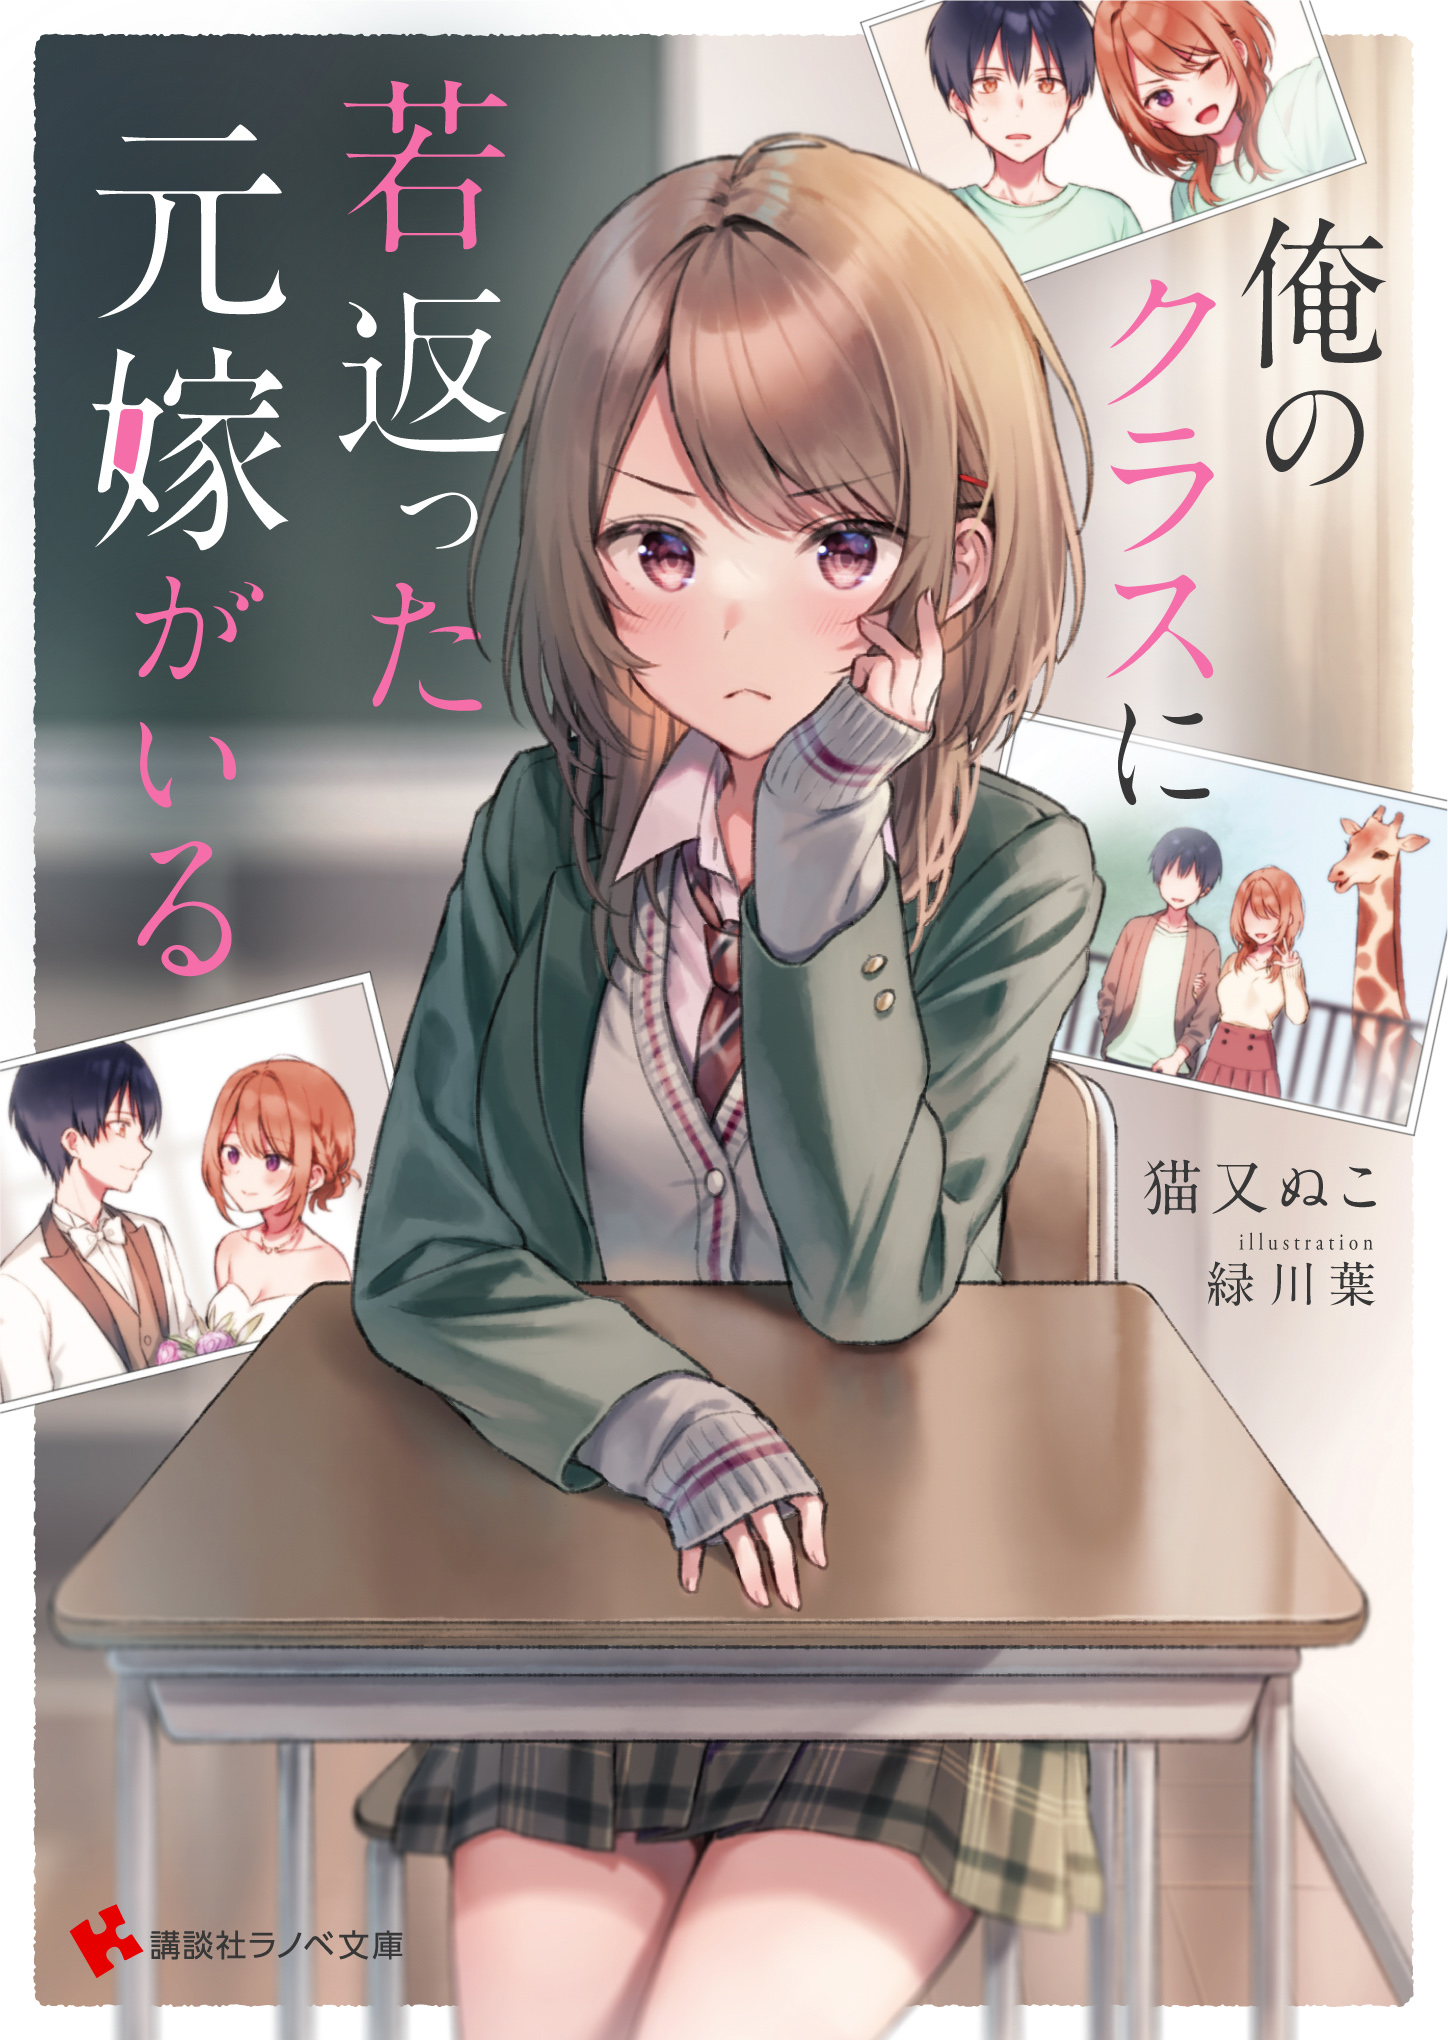
\includepdf[pages=1]{assets/s12096-d89b400d-ce36-47e2-9ca2-a1fa9b674feb-m.jpg}

    \begin{center}
    \textbf{\large Chương 01 \\ Khi tỉnh giấc thì đã trở lại thời thanh xuân}
    \end{center}
    \noindent
“Có hối hận thì cũng trễ rồi nhé!”\\
“Có khóc cũng đã muộn màng rồi nhé!”\\
Buổi chiều tối, trên con đường trở về sau khi đã nộp đơn ly dị.\\
Vừa bước đi trên con đường được ánh đèn đường chiếu tỏ, tôi vừa đấu khẩu với Yuzuka, vợ cũ của mình.\\
Một cuộc ly hôn bất ngờ xuất phát từ chuyện cãi nhau nhỏ nhặt, nhưng mối quan hệ vợ chồng tôi đã trở nên lạnh nhạt mất rồi. Cho dù có từ bỏ chuyện ly hôn lần này đi nữa thì có lẽ sớm hay muộn cũng sẽ thành ra như thế này mà thôi.\\
\\
“Có thể tách ra khỏi cô làm tôi mừng muốn khóc luôn ấy chứ!”\\
“Tôi cũng vậy! Thật mừng khi không phải nhìn mặt anh thêm lần nào nữa!”\\
“Nếu thế này thì thà ly hôn sớm hơn đã tốt rồi! Thế này thì tôi có thể tận hưởng bản hùng ca của sự tự do rồi!”\\
“Nô lệ của công việc như anh thì chẳng có thứ gọi là tự do đâu!”\\
“Chỉ cần không bị sự trói buộc của cô thì đỡ lắm rồi!”\\
“Tôi trói buộc anh khi nào hả!?”\\
“Thì trong lúc tôi đang làm việc cô nhắn tin dai dẳng đến còn gì!”\\
“Chẳng phải do lỗi của anh không trả lời lại à! Đằng này đã làm cơm tối cho rồi thì chí ít anh nhắn lại đi chứ!”\\
“Đang làm thì đâu phải lúc để làm chuyện như thế! Đại khái thì cô cũng hiểu tôi tăng ca mỗi ngày nên không cần cơm tối còn gì!”\\
“Miệng thì nói thế nhưng có lúc anh nhậu nhẹt say xỉn rồi về nhà lúc 8 giờ tối còn gì! Nếu có thời gian đi nhậu thì hãy về nhà sớm đi chứ!”\\
“Chỉ thỉnh thoảng không có tăng ca thôi! Do là cô, mà lại còn đột nhiên nhắn tin đến kiểu$\lfloor$về nhà ăn cơm$\rceil$này nọ nên tôi mới trở nên khó chịu đấy chứ!”\\
“Đằng nào thì anh cũng muốn tận hưởng trong mấy hàng quán có gái gú chứ gì! Vì anh có cái bản tính lăng nhăng mà!”\\
“Cô dai thật đấy! Tôi đã nói đấy không phải lăng nhăng còn gì!”\\
\\
Tôi đã từng nghĩ mình là người hạnh phúc nhất trần đời khi bắt đầu hẹn hò với lại Yuzuka.\\
Và đã từng nghĩ sau khi kết hôn rồi sẽ tiếp tục sống hạnh phúc cả một đời.\\
Vậy mà bước sang năm thứ 4——sang tuổi 27 thì cuộc sống hôn nhân kết thúc.\\
Nếu như có thể gặp được bản thân trong quá khứ thì tôi muốn cho nó lời khuyên. Rằng, đừng có mà kết hôn với con nhỏ đó.\\
\\
“Khoan đã! Đừng có mà đi theo tôi chứ!”\\
“Tôi chỉ đang về nhà thôi!”\\
“Là nhà của tôi mà!”\\
“Nhưng cũng là nhà của tôi còn gì!”\\
“Anh thì đi qua đêm ở quán nét cà phê đi! Anh quen qua đêm rồi còn gì!”\\
“Có phải tôi qua đêm vì tôi muốn qua đêm đâu! Chỉ do lỡ chuyến tàu cuối nên tôi mới qua đêm thôi! Còn cô thì sướng quá nhỉ, tới chiều tối là được về!”\\
“Đừng có chỉ sang tôi! Lỗi do anh làm việc ở công ty đen$^\text{[note43509]}$ mà không phải à!”\\
“Có phải tôi thích rồi đi làm ở đấy đâu! Do công ty trước phá sản, không việc làm sẽ khó coi lắm nên tôi mới vội nhận việc ở công ty đen thôi!”\\
“Không phải tôi đã khuyên anh suy nghĩ cho kỹ rồi hẳn nhận việc à! Anh đúng là chẳng có con mắt nhìn công ty gì cả!”\\
“Cả con mắt nhìn con gái nữa đấy!”\\
“Câu đó tôi nói mới đúng! Nếu như có thể làm lại cuộc đời thì tôi sẽ không kết hôn với anh lần nữa đâu!”\\
“Câu đó tôi nói mới đúng! Nếu như có thể quay ngược thời gian thì tôi sẽ không dính dáng lấy cô thêm một lần nào nữa đâu!”\\
\\
Nếu như kết hôn là nấm mồ của đời người thì tôi như là thứ bò lên từ mộ vậy.\\
Tức là kể từ cái ngày hôm nay, tôi đã được tái sinh.\\
Trời cho cơ hội thứ hai rồi, hãy quên hẳn đi Yuzuka và tận hưởng cuộc sống khoái lạc nào.\\
Vì thế mà tôi muốn tách rời với Yuzuka ra càng sớm.\\
Có cảm giác rằng tôi đã thua khi nhân nhượng cô ta ở đây, nhưng thà qua đêm ở quán nét cà phê đỡ hơn là tạo ra thêm những hồi ức chẳng mấy tốt đẹp.\\
Tôi dừng lại ở trước cột đèn giao thông.\\
\\
“Cô đi thì cứ đi đi.”\\
“Anh đừng có mà bám theo tôi.”\\
“Ai thèm bám hả! Đổi lại cho đến ngày mai cô dọn hết đống hành lý rồi đi khỏi cho tôi.”\\
“Tôi sẽ làm thế. Tôi chẳng muốn ở lại lâu trong căn phòng còn lưu lại mùi của anh đâu.”\\
\\
Quay lưng lại phía tôi rồi thì Yuzuka băng qua vạch kẻ đường.\\
Đây là lần cuối. Tôi sẽ không phải thấy gương mặt của Yuzuka thêm lần nào nữa.\\
Cuộc sống hôn nhân chớp nhoáng với Yuzuka nhanh như là đèn kéo quân vậy. Chỉ một thoáng thôi cũng đủ làm sự hối hận trong tôi cao ngút trời rồi.\\
Tất nhiên, tôi sẽ nói là không bao giờ làm lại một lần nào nữa.\\
Vì làm lại tức là tôi sẽ chỉ thấy viễn cảnh ly hôn ở trước mắt mà thôi.\\
Cả hai vì nhau mà tuyệt đối không liên quan gì đến nhau sẽ tốt hơn.\\
\\
“……Vậy chào nhé.”\\
\\
Tôi lẩm bẩm nói thế thì Yuzuka quay lại.\\
Tuy rằng tối nên tôi đã chẳng thể thấy rõ ràng cho lắm, nhưng mà có thể thấy được gương mặt ấy như là đang trông chờ chuyện gì đó.\\
\\
“Anh vừa nói gì à.”\\
“Có nói gì đâu.”\\
“Nhất định là có nói mà. Nếu có gì muốn nói thì nói rõ ràng ra đi chứ?”\\
“Đã bảo là không có nói mà.”\\
“Có nói!”\\
“Không có nói! Mau về nhà đi——”\\
\\
Chính là lúc đó. Một vật thể màu đen đã xuất hiện ở góc tầm nhìn. Nó thu hẹp khoảng cách với Yuzuka trong một khoảnh khắc mà không hề giảm tốc độ.\\
Lúc nhận ra thì tôi đã lao đến Yuzuka rồi.\\
Khoảnh khắc tiếp theo, cơn chấn động chạy dọc hết toàn thân—\\
\\
     $\mathbin{\blacklozenge}$\\
\\
“Đa———u quáááááá!?”\\
\\
Tôi ngay lập tức bật người dậy.\\
Má trái đang nóng! Đau nữa!\\
\\
“Cuối cùng thì anh đã chịu dậy!”\\
\\
Đứa con gái mặc đồng phục nhìn xuống tôi hiện đang giữ bên má.\\
Nó mặc đồ thủy thủ, mái tóc đen ấy được buộc theo kiểu đuôi ngựa.\\
Giống hệt như em gái tôi lúc còn trẻ vậy……Nhưng tại sao Sana lại ở đây?\\
Hay là em ấy đến thăm tôi sau khi bị xe đụng? Không, nếu là thế thì tại sao nó lại tát tôi chứ? Hay là nó cố làm tôi đang bất tỉnh tỉnh dậy bằng liệu pháp gây sốc gì đó à?\\
Nhưng mà……ngay từ đầu thì cũng chẳng phải là phòng bệnh? Là phòng của tôi mà nhỉ?\\
Tôi, tại sao lại đang ở nhà của ba mẹ chứ?\\
\\
“Làm gì mà anh thẫn thờ thế?”\\
“Làm gì á……Em, là Sana hả?”\\
\\
Yuzuka dường như vẫn liên lạc định kỳ, nhưng lần cuối mà tôi thấy Sana là vào một năm trước. Có thể thấy em ấy trẻ hơn lúc đó.\\
Có lẽ tôi thấy thế là do em ấy đang mặc đồng phục thủy thủ không chừng……nhưng Sana chắc chắn là không có sở thích cosplay. Vậy mà tại sao lại đang mặc đồng phục chứ?\\
\\
“Đương nhiên em là Sana rồi. Đừng có ngủ mớ nữa, mau chóng dậy đi.”\\
“Dậy đi á, em……”\\
\\
Tôi muốn nói là ‘anh đang bị thương nặng do xe đụng đấy’ nhưng chẳng có cơn đau nào khác ngoài gò má cả.\\
Lành lặn một cách thần kỳ sao? Nếu thế thì——\\
\\
“Nà, nà~, Yuzuka sao rồi? Con nhỏ đó cũng không sao chứ?”\\
“Yuzuka? Ai thế.”\\
“Ai là ai, vợ anh chứ ai——Mà không phải, vợ cũ ấy.”\\
“Anh đang nói về game hả?”\\
“Hiện thực cơ!”\\
“Anh chơi game nhiều quá mức nên không phân biệt được hiện thực với ảo tưởng rồi à……”\\
“Đừng có nhìn anh bằng cái ánh mắt nhìn mấy thứ đáng thương coi!”\\
“Không sao đâu, em là đồng minh của nii-chan! Dù anh có nói kết hôn với lại con gái trong game đi nữa, em cũng sẽ ủng hộ anh!”\\
“Chí ít thì hãy ủng hộ anh có thể gặp được đứa con gái dễ thương giùm cái!”\\
“Nếu thế thì anh phải mau chóng thức dậy! Chúc anh gặp được duyên tốt nè~!”\\
\\
*Bộp*, Sana vỗ vào lưng tôi như thể rót thêm tinh thần rồi bước ra khỏi.\\
Rốt cuộc thì chuyện của Yuzuka và bộ đồng phục thủy thủ vẫn mãi là bí ẩn.\\
Tôi rời khỏi giường mà vẫn chẳng hiểu lý do……rồi chợt nhận ra cảm giác khó chịu.\\
\\
“……không đúng.”\\
\\
Là phòng của tôi, nhưng lại chẳng là phòng của tôi.\\
Cách bố trí của kệ sách khác này, còn được dán cả mấy ảnh poster hoài niệm nữa, có cả những món đồ anime mà chắc chắn rằng tôi đã chuyển đến nhà mới.\\
Yuzuka đã chuyển nó về nhà ba mẹ hay gì đó à?\\
Nếu như thế thì cũng lạ thật. Nếu là thế thì chắc chắn Sana đã nói một lời rồi. Vậy mà Sana còn nói là không biết Yuzuka chứ đừng bảo là giải thích sự tình.\\
Bọn họ thân thiết với nhau lắm, vậy mà rốt cuộc tại sao lại giả vờ không biết nhau chứ?\\
Cảm giác như tôi đã lạc vào thế giới song song vậy.\\
Tôi bước xuống lầu 1 trong khi vẫn chẳng hiểu sự tình thì cả gia đình đã tập trung tại phòng ăn rồi.\\
\\
“……Hả?”\\
“Sao thế Kouhei, làm gì ngẩn người ra thế.”\\
“Không mau ăn là súp miso sẽ nguội đi đấy.”\\
“C-, con là người nói sao thế mới đúng! Tại sao mẹ lại trẻ lại thế này!?”\\
“Hôm nay mẹ trang điểm gọn gàng ấy mà.”\\
“Nó vượt qua cái đẳng cấp đánh lừa bằng trang điểm rồi đấy! Trông mẹ trẻ hơn thật luôn đó!”\\
“Á rà, khéo khen ghê.”\\
“Con có khen gì đâu! Còn tóc của ba thì trở nên rậm rạp hơn này!”\\
“Có lẽ hiệu quả của thuốc mọc tóc tốt chăng.”\\
“Nó vượt quá mức của thuốc mọc tóc rồi đấy!”\\
\\
Chẳng phải giống với ông bố trong bộ Gia đình Hải Sản$^\text{[note43508]}$ luôn rồi à!\\
\\
“Nii-chan Nii-chan!”\\
“Gì đấy!”\\
“Em thì sao? Anh không có gì để khen ư!”\\
“Bộ đồng phục cũng hợp với em lắm!”\\
“Hoan hô~! Con được nii-chan khen này!”\\
“Thích rồi nhé, Sana-chan.”\\
“Kouhei hôm nay có tâm trạng muốn khen nhể. Được, vậy thì ba cũng thế luôn. Bữa sáng của mẹ nó hôm nay cũng ngon lắm ghê ha.”\\
“Cách mẹ nướng xúc xích là số dách ạ!”\\
\\
Đừng có bỏ mặc tôi rồi khen lấy khen để nhau giùm với!\\
\\
“Làm ơn giải thích cho con đi mà! Mẹ à, tại sao mẹ lại trẻ lại thế!? Ba à, tại sao tóc ba lại rậm rạp thế!? Sana à, tại sao em lại đang mặc đồng phục thế!?”\\
“Thì hôm nay là ngày đến trường mà.”\\
“Con cũng mau đi rửa mặt đi. Cũng chải đầu cổ rối tung gọn gàng lại. Vì hôm nay là ngày quan trọng đấy.”\\
“……Ngày quan trọng là sao?”\\
\\
Tôi đang bối rối rồi, mẹ lại nói ra thêm một câu càng làm tôi bối rối hơn.\\
\\
“Thì là lễ nhập học cao trung mà.”\\
-OoO-\\
Đọc bản dịch gốc và ủng hộ nhóm dịch tại \href{https://ln.hako.re/}{ln.hako.re}\\
\newpage

    \begin{center}
    \textbf{\large Chương 02 \\ Có nhỏ vợ cũ đã hồi xuân}
    \end{center}
    \noindent
Trời đầy mây.\\
Nhìn lên mái trường trông đã cũ kĩ vì bề dày lịch sử này, tôi lại ngập tràn thứ cảm xúc chẳng thể tin được ở trong lòng.\\
\\
“Làm gì ngờ được có ngày mình lại đến tới đây chứ……”\\
\\
Cho đến hôm qua tôi vẫn là một người trưởng thành 27 tuổi, vậy mà khi mở mắt dậy đã trở thành học sinh cao trung năm nhất thế này, có mơ cũng chẳng nghĩ đến.\\
Tôi đã thử nhéo gò má mình biết bao nhiêu lần để xem có phải là mơ không, nhưng đã chẳng tỉnh dậy. Chuyện khó tin đấy, nhưng thật sự là tôi đã xuyên không về quá khứ.\\
Cái này là may mắn, hay là bất hạnh đây—\\
Và tôi đã xem như nó là may mắn.\\
Dù sao đi nữa, nếu như đây là giấc mơ thì tôi ở hiện thực đã bị một chiếc xe chạy ẩu đâm phải, và hiện đang lang thang giữa ranh giới sinh tử.\\
Hơn hết thì nếu như có thể làm lại từ thời cao trung, chỉ cần không tham gia vào đời sống hôn nhân là xong.\\
Cuộc đời thứ hai này, mình sẽ đi làm ở một công ty đàng hoàng, rồi trở thành quý tộc độc thân cho xem!\\
Tôi hồi hộp bước qua cổng trường, tiến đến lối ra về nơi để giày.\\
Thử xác nhận danh sách phân chia lớp được dán ở chỗ để giày, tôi học lớp 1 đúng như dự đoán. Và theo như trí nhớ thì bên dưới cái tên Kurose Kouhei có cái tên Koikawa Yuzuka.\\
Tuy là thứ tự ghế khá gần, nhưng không liên quan đến Yuzuka là chuyện đơn giản thôi.\\
Tôi và Yuzuka 3 năm liên tiếp học cùng lớp, nhưng cuộc nói chuyện đầu tiên là kể từ sau khi tốt nghiệp cơ.\\
Tất cả bắt đầu khi mà chúng tôi cùng dự chung một bài giảng ở mái trường đại học rất xa, lại tình cờ ngồi cạnh nhau nữa.\\
Nếu như không học lên cùng chung một trường đại học—nếu như không dự chung bài giảng thì tôi sẽ chẳng liên quan gì đến Yuzuka này, hay cho dù chẳng làm đến tận như thế đi nữa, chỉ cần không có mối quan hệ thân mật là có thể tránh được cái tuyến đường kết hôn thôi.\\
\\
“Chiến thắng quá dễ.”\\
\\
Khi nghĩ như thế thì cảm xúc dễ chịu thật.\\
Do thời cao trung chẳng có giao lưu với nhau, nên là tôi có thể tận hưởng thời kỳ thanh xuân mà chẳng phải lo lắng gì cho đến lúc tốt nghiệp cả.\\
……Dù nói là thanh xuân đi nữa, tôi đã chẳng hề có bè bạn. Ừ thì, khác với người trưởng thành ở chỗ tôi có rất nhiều thời gian. Chỉ cần chơi game thôi là có thể tận hưởng nhỉ.\\
Tôi thay giày rồi tiến đến lớp 1 năm nhất.\\
Cả lớp gần như đã tập hợp đông đủ, trong số đó cũng có Yuzuka nữa.\\
Tuy phong cách của trường là tự do, nhưng chỉ mỗi Yuzuka là đang nhuộm tóc. Mái tóc màu nâu sáng, vẻ mặt mang ý chí mạnh mẽ, ánh mắt thì sắc bén, ngực to……thật bực khi phải thừa nhận, nhưng mà cô ta đúng là người đẹp.\\
Thậm chí chẳng có người quen, vậy mà do vẻ bề ngoài hoàn toàn khiến cô ta lạc lõng với xung quanh.\\
\\
“……”\\
\\
Chết rồi! Chạm phải ánh mắt với Yuzuka mất rồi!\\
Tôi có cảm giác tội lỗi khi mà lơ đi Yuzuka của đường thế giới này, nhưng nếu đôi bên dính dáng lấy nhau thì sẽ chẳng có gì tốt đẹp cả.\\
Nếu như tôi có cúi chào thì có lẽ đành phải bắt đầu những ngày tháng khác biệt với thời cao trung mà tôi biết.\\
Tôi nhanh chóng lảng ánh nhìn đi rồi đến chỗ ngồi, rồi vờ ngủ để mặc kệ.\\
Đã chẳng một đứa nào đến bắt chuyện với con người tôi như thế cả. Cũng có mấy đứa học cùng trường trung học, nhưng mà bọn nó đã lập nhóm hết cả rồi.\\
Nếu tôi lấy dũng khí rồi hành động thì có lẽ những ngày tháng bạn bè sẽ đến đấy, nhưng cảm giác là tất cả bọn nó đều dưới tuổi tôi. Tôi không nghĩ mình sẽ có thể bắt kịp chúng nó đâu.\\
\\
“……”\\
\\
Dù là thế nhưng lại chẳng thể bình tĩnh nổi.\\
Người ở đằng sau không phải là vợ cũ, mà là bạn cùng lớp.\\
Trong đầu tôi đã hiểu như thế rồi, vậy mà chẳng thể ngơi nghỉ một tí nào.\\
Kíng kong kang kong——!\\
Hồi chuông hoài niệm vang lên, được một hồi thì giáo viên đến.\\
Là một cô giáo rất hiền hậu. Không nhầm thì……là Sawashiro-sensei phải không nhỉ?\\
Hoài niệm ghê ta. Đương thời có thể trông cô ấy trưởng thành, vậy mà bây giờ tôi lại lớn tuổi hơn.\\
Chuyện cô giáo là người dưới tuổi mình cảm giác kỳ lạ sao ấy nhỉ.\\
Nói lại lời chúc mừng sau khi nhập học, giải thích xong lịch trình của ngày đầu hôm nay rồi thì Sawashiro-sensei vui vẻ nói.\\
\\
“Nào. Trước khi di chuyển đến hội trường, mọi người hãy đơn giản giới thiệu bản thân cho cô nhé! Hãy lên bục theo thứ tự ghế của bản thân!”\\
\\
Aoki-kun, Inoue-san, Etou-san, Ooishi-kun, toàn những gương mặt thân quen hoài niệm lần lượt bước lên, làm tôi một lần nữa cảm nhận thực tế chuyện xuyên không về quá khứ.\\
Đến lượt thì tôi bước lên bục giảng.\\
Vừa tránh nhìn Yuzuka, tôi vừa giới thiệu bản thân một cách nhạt nhẽo.\\
\\
“Tớ là Kurose Kouhei đến từ trường trung học Botan. Sở thích là đọc sách. Và……tớ cũng thích xem phim nữa, một tháng tớ cố đến rạp phim một lần. Một năm tới đây mong các bạn chiếu cố.”\\
\\
Tôi trở về chỗ sau những tràng pháo tay.\\
Tiếp theo là đến lượt Yuzuka.\\
Cô ta đứng trên bục giảng, nhìn xung quanh lớp học. Quả đúng là người giành được hợp đồng làm việc từ nhiều công ty, dáng vẻ đường đường chính chính khiến cho người ta cảm thấy một phần như thế.\\
Ừ thì sự hiên ngang đó chỉ là vẻ bề ngoài thôi, chứ cô ta khá là sợ đám đông đấy.\\
Cứ hồi hộp là cô ta ăn nói bập bẹ, ngay lập tức lẹo lưỡi, nên không nhầm thì mỗi ngày đều cùng tôi luyện tập phỏng vấn nhỉ. Chuyện đó cũng có giá trị khi mà cô ta dần trở nên ăn nói rành rọt này, khác hẳn với tôi là cô ta chưa từng nhận được thư từ chối nhận việc nào cả.\\
Yuzuka ở đường thế giới này có lẽ sẽ vất vả khi xin việc ha.\\
Tôi cảm thấy trông tội nghiệp một chút, nhưng để cô ta nhận được thư từ chối đỡ hơn là bản thân mình dấn vào cuộc sống hôn nhân đó.\\
Khi tôi đang nghĩ đại loại như thế thì Yuzuka xưng tên bằng giọng nói rất là truyền cảm.\\
\\
“Tôi đến từ trường trung học Kirishima, Kurose Yuzuka.”\\
\\
……Ể?\\
Cô ta vừa nói gì cơ!?\\
Mình nghe lầm à? Có cảm giác cô ta xưng tên mà cùng họ với tôi ấy……\\
Vả lại còn bằng giọng nói rõ ràng, không khiến tôi cảm nhận được sự hồi hộp ấy chứ.\\
Yuzuka cứ thế mà định tiếp tục giới thiệu bản thân thì Sawashiro-sensei bảo chờ đã.\\
\\
“Etou……Em vừa nói là Kurose?”\\
“Vâng. Kurose Yuzu……Không phải! Koikawa! Koikawa Yuzuka ạ!”\\
\\
Yuzuka đỏ mặt.\\
Cô ta vội vàng đảo ánh mắt, loáng thoáng nhìn đến chỗ tôi.\\
\\
“C-, ch-, ano……em xin lỗi, gia đình em gặp phải nhiều chuyện……tinh thần em vẫn chưa ổn định được ạ……”\\
“A, aa, ra là……Được mà, em không cần phải xin lỗi đâu.”\\
\\
Sawashiro-sensei nói như thể quan tâm.\\
Khi nghe cái lời giải thích ‘gia đình em gặp phải nhiều chuyện’ đó thì mọi người ai cũng làm cái bộ dạng hiểu theo kiểu$\lfloor$ba mẹ ly hôn nên có lẽ mới đổi họ$\rceil$, nhưng—\\
Cái này, chính là nó mà đúng chứ?\\
Là như thế mà……ha?\\
\\
“Rồi, cảm ơn em, Koikawa-san. Vậy xin mời bạn tiếp theo.”\\
\\
Yuzuka sau khi kết thúc phần giới thiệu bản thân thì vừa loáng thoáng nhìn qua tôi, vừa quay về chỗ mà trông như xấu hổ.\\
Tôi bằng cách nào đó đã vượt qua bằng vẻ mặt tỉnh bơ, nhưng tim thì lại đang loạn nhịp.\\
Không thể bắt chuyện ngay bây giờ và tại đây được.\\
Cũng chẳng thể bắt chuyện khi mà chỉ còn có hai đứa.\\
Nên tôi đã hét lên trong lòng mình.\\
\\
Thế ra mẹ trẻ cũng xuyên không về quá khứ á!\\
-OoO-\\
Đọc bản dịch gốc và ủng hộ nhóm dịch tại \href{https://ln.hako.re/}{ln.hako.re}\\
\newpage

    \begin{center}
    \textbf{\large Chương 03 \\ Nhỏ vợ cũ cứ xà nẹo lại gần}
    \end{center}
    \noindent
Dù cho đến lúc lễ nhập học kết thúc đi nữa thì con tim tôi vẫn đang đập inh ỏi.\\
Khi nghĩ đến người ngồi ở bàn sau không phải là Yuzuka thời cao trung, mà là người vợ Yuzuka thường hay lặp đi lặp lại chuyện cãi nhau khiến tôi không thể bình tĩnh nổi.\\
May mắn thay là Yuzuka không biết chuyện tôi xuyên không về quá khứ. Miễn là không dở hơi như Yuzuka thì tôi có thể vượt qua mà không bị phát hiện.\\
Nhưng mà, khi nghĩ đến chuyện nếu bị phát hiện……rồi nghĩ đến chuyện phải sống cuộc sống học đường tù túng với vợ cũ trong lớp học chật hẹp thì tôi trở nên tuyệt vọng.\\
Nếu thành thế này thì phải chú tâm diễn cho giống như ở đường thế giới cũ!\\
Tôi và Yuzuka liên quan đến nhau là sau khi tốt nghiệp nên cho dù không hoàn toàn giống đi chăng nữa thì cũng chẳng lộ ngay tức thì được, nhưng phải cẩn thận để không đi lệch hướng quá lớn.\\
\\
“Mọi người xin hãy chú ý~”\\
\\
Sawashiro-sensei vỗ tay bộp bộp thu hút ánh nhìn.\\
Kết thúc lễ nhập học, sự căng thẳng đã được giải tỏa, hay đám bạn cùng lớp an tâm khi đã có thể trò chuyện thân mật với nhau hay sao mà bầu không khí của lớp thả lỏng hơn.\\
Để thúc đẩy sự lơi lỏng đó mà Sawashiro-sensei nở nụ cười thật tươi và tiếp tục nói.\\
\\
“Từ giờ cô sẽ phát bản in, nên các em hãy chuyền xuống bàn dưới nhé. Trên đó có viết lịch trình của tháng này, nên là hãy đọc cho kỹ nhé.”\\
\\
Truyền tay bản lịch trình tháng này. Tôi cũng phải xác nhận cho kỹ để nhớ lại thời học sinh nữa.\\
Khi nhìn gương mặt của Yuzuka có thể sẽ bị cô ta biết tôi dao động nên khi mà tôi định đưa cái bản in nhận được từ Kikuchi-san mà không nhìn ra đằng sau thì—\\
~\\
\\
“——~!?”\\
\\
Ngón tay bọn tôi chạm vào nhau, khiến toàn thân giật run.\\
B-, bình tĩnh nào tôi ơi! Yuzuka là vợ cũ đó! Đừng có mà dao động chỉ vì ngón tay chạm vào nhau ngay lúc này chứ!\\
Cơ mà có thể nói là may mắn hay gì đó. Do là phản ứng giống với một nam sinh cao trung chưa từng bao giờ được chạm vào con gái, nên tôi đã chẳng bị Yuzuka ngờ vực—\\
Cũng chẳng bị gọi ở lại nên là tôi cứ thế mà rời khỏi lớp học sau giờ tan trường.\\
Phóng ra khỏi cổng trường rồi thì tôi thở dài.\\
\\
“Phù~……”\\
\\
Trước hết thì vượt qua rồi hen.\\
Cuộc sống học đường với người vợ cũ sẽ chính thức bắt đầu sau 3 ngày tính cả thứ bảy và chủ nhật, nhưng hôm nay tạm thời an tâm rồi.\\
Thời gian thì có rất nhiều, hay là mình tận hưởng cuộc sống game thủ đã từ lâu lắm rồi để lấy lại sự bình tâm nhỉ.\\
Quyết định thế rồi thì tôi nhanh chóng quay về nhà, nhưng……\\
\\
“……Nhắc mới nhớ mình vẫn xài điện thoại gập nhỉ.”\\
\\
Thời này thì đã có smartphone rồi, nhưng nó chỉ mới được ra mắt vào dịp tôi nhập học cao trung mà thôi.\\
Smartphone nổi lên trên thị trường cũng phải vài năm sau. Đột nhiên có đổi thì cũng chẳng thể chơi được.\\
Mà, thôi kệ vậy. Có game cố định kia mà.\\
Tôi khởi động cái máy game 2 thế hệ trước rồi chơi cái game đã từng chơi.\\
Điều khiển tướng rồi đi chặt pặc pặc mấy tên lính lác lôm côm.\\
\\
“……”\\
\\
Đương thời thì tôi ấn tượng do nó hệt như người đóng vậy, nhưng bây giờ nhìn thì đồ họa thô gì đâu. Khi sử dụng kỹ năng tất sát thì ảnh chuyện động khá chậm……quá stress luôn chứ.\\
Được 10 phút thì tôi chán, đổi đi đổi lại rồi chơi mấy cái game cũ hoài niệm nhưng lại chẳng có động lực mấy.\\
Tra mấy game trông thú vị trên mạng thì đập vào mắt tôi là game online.\\
Hồi đó thì có rất nhiều game mà tôi muốn chơi, và tôi đã tránh chơi mấy cái game online mà trông như sẽ làm mình phân tâm rồi chẳng biết rằng thời gian đã trôi qua, nhưng mà cũng có mấy khi có được cuộc đời lần thứ hai đâu chứ. Chơi mấy game mà lần trước đã chẳng thể chơi trông cũng thú vị đấy.\\
Vấn đề là tiền bạc cơ.\\
Nếu như theo trí nhớ của tôi thì mùa xuân này có game mới rất là phong phú, tiền tiết kiệm thì chắc chắn đã cạn. Tiền tiêu vặt mỗi tháng được 6000 yên. Nửa trong số đó trừ vào tiền điện thoại rồi nên nếu muốn mua game thì sớm nhất cũng phải tháng tới nữa.\\
\\
“……Thôi thì đến tiệm sách nhỉ.”\\
\\
Mua Light Novel rồi giết thời gian thôi.\\
Tôi mặc quần áo thường ngày và định ra khỏi phòng……thì chợt nhớ ra.\\
\\
“Hôm nay, là ngày giỗ của cái máy tính phải không ta?”\\
\\
Không nhầm thì đúng là thế.\\
Tuy là tôi không trực tiếp nhìn thấy, nhưng mà ai đó (có lẽ là Sana) đã nói là có sét giáng xuống công viên lân cận.\\
Chính do đó mà cái máy tính bị hư, và tôi buộc phải từ bỏ game mới một thời gian.\\
\\
“Cảm giác lời ghê ha.”\\
\\
Tôi rút ổ cắm, thực hiện mấy cái kế sách chống sét đánh xong rồi cầm theo dù bước ra ngoài.\\
Đi bộ khoảng 30 phút thì đến nhà sách gần nhất.\\
Manga, Light Novel hay CD gì đó đều có, là một cửa tiệm mà như thể hiện thân cho lý tưởng của con nít vậy.\\
\\
“Hoài niệm thật ha.”\\
\\
Mùa đông năm 2 đại học, cửa hàng này làm ăn thất thu mà bị phá sản.\\
Lúc đó tôi thật sự thất vọng não nề. Bởi vì nó là nhà sách của kỷ niệm, nơi mà tôi đã từng lui đến kể từ lúc còn nhỏ mà.\\
Nếu như máy tính không bị hư và tôi có thể đổ tiền vào thì doanh số bán hàng có thể tăng được thêm một chút. Sự khác biệt nhỏ nhặt đó có thể làm cho cửa tiệm không bị phá sản không chừng.\\
Tôi vừa nghĩ như thế, vừa bước vào trong cửa tiệm hoài niệm.\\
\\
“Ge~”\\
\\
Yuzuka đang ở quầy manga.\\
Tại sao con nhỏ này lại ở đây chứ! Cô chẳng phải nói với tôi là thường mua sách ở trung tâm mua sắm cho đến khi hẹn hò với tôi à!\\
Tôi là người đã chỉ cho Yuzuka tiệm sách này. Lúc đó là thì nó đã đóng cửa rồi. Thế nên cô ta đến để xem nó như thế nào sao?\\
Không, cho dù có như thế thì tôi cũng chẳng hiểu lý do mà cô ta đến tiệm sách mà tôi đã chỉ cho. Bởi vì Yuzuka ghét tôi mà. Chắc chắn đối với Yuzuka thì tiệm sách này phải là nơi mà cô ta ghét bỏ chứ……\\
……Ừ thì, tiệm sách đâu có tội tình gì đâu ha.\\
Nếu không có gì để mua ngoài sách thì cửa tiệm này gần hơn, nên chuyện cô ta đến đây tôi cũng chịu thuyết phục đó.\\
Nói chung là bơ đi.\\
Phải vờ như là chẳng nhìn thấy, như là tôi ở trong đường thế giới này.\\
Dù đã quyết định như thế nhưng tôi không muốn tiến về phía của Yuzuka tí nào, nên đã dành thời gian ở quầy game.\\
Rồi thì——\\
\\
“……A.”\\
\\
Yuzuka đi đến đây.\\
Cô ta nhìn mặt tôi rồi$\lfloor$A$\rceil$gì đó lên một tiếng.\\
Nếu trải qua vài ngày sau lễ nhập học mà không phản ứng thì ngược lại sẽ thiếu tự nhiên, nhưng hôm nay là ngày đầu tiên nhập học. Không nhớ mặt bạn bè trong lớp cũng chẳng có gì thiếu tự nhiên cả!\\
\\
“Cậu là……Kurose-kun nhỉ?”\\
\\
Tại sao lại bắt chuyện chứ!\\
Tôi đã làm lơ đi rồi vậy mà!\\
Mà trắng trợn thật ha. Cái gì mà$\lfloor$Cậu là……Kurose-kun nhỉ?$\rceil$vậy hả.\\
Là một cái tên mà cô muốn quên mà quên cũng không được còn gì.\\
\\
“E, etto……cậu là ai?”\\
“Tớ ngồi bàn sau……hora, là cái người đã ăn nói kì cục lúc giới thiệu bản thân đó.”\\
“X-, xin lỗi. Hôm qua tớ thức đêm để cày game nên lúc đã ngủ hết nửa phần trong buổi giới thiệu bản thân mất.”\\
“Vậy ư. Rất giống với lại Kurose-kun nhỉ.”\\
“……Rất giống với Kurose-kun? Hôm nay chắc hẳn là lần đầu chúng ta gặp mặt mà nhỉ……”\\
“A~, xin lỗi. Là chuyện của tớ. Cậu đừng có bận tâm.”\\
\\
Nguy hiểm, nguy hiểm quá.\\
Mới nãy mình lơ là quá, suýt nữa thì bị Yuzuka nghi ngờ rồi.\\
\\
“Cậu chơi loại game thế nào thế, Kurose-kun?”\\
“T-, tại sao?”\\
“Tớ cũng có chơi game đó, nên nếu như cậu có game nào muốn giới thiệu thì tớ muốn cậu chỉ cho ấy mà.”\\
\\
Gì, tại sao lại muốn hỏi tôi chứ!?\\
Tại sao lại xáp xáp vào tôi vậy hả!?\\
Dù đường thế giới có khác thì tôi vẫn là tôi đó! Là Kurose Kouhei mà cô cực kỳ ghét đó!?\\
Khó khăn lắm mới làm lại cuộc đời vậy mà cớ sao lại cố dính dáng đến tôi vậy hả!?\\
Tôi giới thiệu cho cô ta vài cái tựa game dù cho bản thân vẫn không hiểu rõ ý.\\
Rồi thì—\\
\\
“Cái đó tớ cũng thích lắm~!”\\
\\
Và Yuzuka đã nở nụ cười tươi rói.\\
Nụ cười đó làm tôi chợt rung động.\\
Đã bao lâu rồi mới thấy lại nụ cười của Yuzuka ấy nhỉ. Bất chợt khiến tôi nghĩ rằng thật là dễ thương……\\
Tôi nhớ lại câu lăng mạ ‘tôi thà ở với gián còn đỡ hơn anh’ rồi kìm nén sự rung động lại.\\
\\
“Tớ cũng thích game đi săn nữa, nhưng đặc biệt là game Musou tớ đã chơi hơn 100 tiếng rồi. Tất cả các tướng đều Max Status cả, cũng nắm rõ ở đâu trên Map có vật phẩm nữa đó.”\\
“Hể, hể~, ra là vậy. Koikawa-san cũng chơi game nhiều thật ha.”\\
\\
Còn tôi thì đã chơi hơn 300 tiếng rồi.\\
\\
“Cậu ngạc nhiên sao?”\\
“Ừ thì……Ngạc nhiên chăng.”\\
“Bởi vì vẻ ngoài tớ giống yankee sao? Tớ, hoàn toàn chẳng đáng sợ đâu.”\\
\\
Đáng sợ quá.\\
Bình thường không đáng sợ nhưng lúc cãi nhau thì cực kỳ luôn ấy. Khi người đẹp mà nổi cáu thì nó lại tăng thêm 50% cơ.\\
\\
“Vừa rồi tớ không có lườm cậu đâu. Ánh nhìn của tớ xấu là do thị lực tớ kém thôi.”\\
“R-, ra là vậy.”\\
\\
Tôi biết chứ.\\
Yuzuka xuất thân từ vùng quê, hiện tại đang sống một mình tách rời với lại cha mẹ.\\
Vốn dĩ cô ta là đứa con gái quê mùa với mái tóc đen và cặp kính như hàng mẫu vậy, nhưng để không bị chọc là dân nhà quê mà cô ta ra mắt bản thân ở trường cao trung—bằng mái tóc đã nhuộm và tháo rời cặp kính xuống.\\
Vậy mà cô ta chẳng thèm đeo kính áp tròng. Vì cô ta sợ dị vật lọt vào mắt gì đó.\\
Lúc nghe chuyện đó, tôi đã nói$\lfloor$dễ thương ghê$\rceil$và cô ta thì trở nên ngượng ngùng, nhưng bây giờ thì chỉ có thể đơn thuần nghĩ rằng$\lfloor$mẹ trẻ đeo kính vào đê$\rceil$mà thôi.\\
\\
“Cậu không đeo kính sao?”\\
“Tớ định chỉ đeo kính trong giờ học mà thôi.”\\
“Nhưng mà thị lực của cậu kém mà đúng chứ?”\\
“Thế này thì chỉ cần ghé sát mặt lại gần là có thể nhìn thấy đó.”\\
\\
Kh- wa~! Đừng có đột nhiên ghé sát mặt lại gần coi!\\
T-, tôi sẽ hồi hộp mất……\\
\\
“Gương mặt của Kurose-kun, trẻ ghê.”\\
“Ừ, ừ thì tớ cũng là học sinh cao trung rồi mà.”\\
\\
Đừng có nói chuyện với khoảng cách gần như này giúp tôi.\\
Hơi thở của cô ngọt quá đấy. Với lại bộ ngực to trông như sắp chạm vào rồi kìa……!\\
\\
“Nhân tiện thì, cậu là con một sao Kurose-kun?”\\
“Tớ có một đứa em gái……”\\
“Ra là cậu có em gái~!”\\
\\
Gương mặt của Yuzuka sáng rỡ.\\
……Ra vậy. Xáp xáp lại cái đứa mà cô ta ghét là tôi đây để làm thân với lại Sana à.\\
Hai đứa nó thân đến mức bỏ tôi lại một mình rồi đi chơi luôn mà.\\
\\
“Em ấy tên gì thế?”\\
“Sana.”\\
“Là Sana-chan à~. Cái tên dễ thương ghê~. Em ấy là người thế nào? Có ảnh không?”\\
“Không có.”\\
“Thế à. Tớ muốn xem ghê~”\\
\\
Nếu như tôi muốn lấy le với con gái thì để gần gũi hơn với Yuzuka sẽ mời cô ta đến nhà rồi, nhưng bọn tôi chỉ mới ly hôn có nửa ngày trước mà thôi.\\
Ngay từ đầu thì tôi chẳng định dính dáng gì với Yuzuka cả.\\
Chuyện mời cổ đến nhà đúng là một sai lầm ngớ ngẩn.\\
\\
“Xin lỗi. Em gái tớ, có sinh hoạt câu lạc bộ rồi.”\\
“Câu lạc bộ nào thế?”\\
“Câu lạc bộ bóng rổ.”\\
\\
Chẳng phải lý do nó thích bóng rổ đâu, chỉ là nó gia nhập câu lạc bộ vì nghe được chuyện nếu chơi bóng rổ sẽ cao lên thôi.\\
Rốt cuộc thì đã chẳng cao lên, nhưng dường như nó đã trở nên thích bóng rổ mà tiếp tục chơi cho đến khi vào đại học.\\
\\
“Nói chung là như thế đấy, nên nếu cậu muốn gặp em gái tớ thì có thể đi cổ vũ mấy trận đấu là được. V-, vậy nhé, tớ xem manga đây!”\\
\\
Tôi ngay lập tức rời đi.\\
Đã cảnh giác vì có lẽ sẽ bị bám theo, nhưng mà bóng dáng của Yuzuka đã biến mất khỏi tiệm rồi.\\
-OoO-\\
Đọc bản dịch gốc và ủng hộ nhóm dịch tại \href{https://ln.hako.re/}{ln.hako.re}\\
\newpage

    \begin{center}
    \textbf{\large Chương 04 \\ Đã quyết định không vướng bận lấy nhau vậy mà}
    \end{center}
    \noindent
Khi tôi bước khỏi hiệu sách thì trời đã bắt đầu mưa.\\
Sắc trời nhìn như là một cơn mưa lớn thật sự sẽ trút nước từ bây giờ.\\
\\
“Làm sao bây giờ đây ta……”\\
\\
Nếu ở tiệm sách thì có tôi có thể dành vài tiếng để giết thời gian. Sau khi tạnh mưa thì về cũng được, nhưng tôi vẫn chưa dùng bữa trưa.\\
Đã quá 2 giờ trưa rồi. Quả thật bụng cũng đang réo nữa chứ.\\
Tôi biết là sét sẽ đánh xuống, nhưng không biết đến mấy giờ thì trời sẽ tạnh mưa. Thôi thì mau chóng về nhà dùng bữa vậy.\\
Chẳng mấy chốc sau khi rời hiệu sách, cơn mưa dần nặng hạt hơn.\\
Tôi không muốn những giọt nước mưa nguội lạnh thấm vào giày tí nào. Khi tôi nhanh chân bước đi cùng với những giọt mưa tí tách thì trời bắt đầu gầm gừ tiếng sấm.\\
Do biết thông tin sét đánh nên tôi cũng ngại băng qua trước công viên, nhưng nhà tôi lại ngay trước nó. Tất yếu phải đi ngang qua rồi.\\
Tôi chạy qua công viên với nỗi bất an cùng với nhịp tim đang tăng lên nhanh chóng—\\
\\
“……”\\
\\
Tôi thấy có ai đó ở góc tầm nhìn.\\
Ở bên kia hàng rào đan với cây thường xuân——Yuzuka hiện đang có mặt tại nơi nghỉ chân có mái che.\\
Cổ đang co người lại, bịt lấy hai tai.\\
Con nhỏ này, đang làm gì ở công viên thế……\\
Nhà của Yuzuka là một căn hộ cách nơi này 10 phút đi bộ. Từ tiệm sách đến khu căn hộ có rất nhiều tuyến đường, và lối tắt chính là băng qua công viên.\\
Tôi hiểu cô ta chọn con đường tắt để quay về cho nhanh, nhưng nếu thế thì tại sao lại sao cô ta lại ở công viên chứ?\\
Yuzuka cực kỳ sợ sấm sét.\\
Khi mà mối quan hệ vợ chồng còn tốt đẹp, mỗi khi nghe tiếng sấm là cô ta dính chặt lấy tôi, còn lúc cãi nhau thì tôi đã quan tâm mà ngủ ở ngoài sô-pha rồi, vậy mà lại đến làm nũng$\lfloor$đến giường đi mà$\rceil$với tôi.\\
Sợ sấm thì đừng có trú ở công viên chứ, mau chóng về lẹ đi là được mà……\\
Đám mây đen lóe sáng, tiếng sấm vang lên chói cả tai. Dù bịt tai nhưng chắc là vẫn nghe nên Yuzuka dần co người lại hơn.\\
……Mình đã quyết định là không dính líu đến Yuzuka rồi. Dù cô ta có đến bám vào đi nữa thì tôi cũng chẳng bao giờ vướng mắc đến cô ta đâu.\\
Nhưng mà……chuyện ở ngay công viên đúng lúc thế này, rõ là cô ta không biết chuyện sét đánh xuống nhỉ.\\
Có khả năng nó sẽ đánh trực diện xuống nhà nghỉ, quả nhiên không thể ngó lơ được nhỉ.\\
Sau khi thở dài lấy một hơi rồi thì tôi bước vào công viên và bắt chuyện với cô ta từ đằng sau.\\
\\
“……Koikawa-san?”\\
“……”\\
“Koikawa-san.”\\
“……”\\
“Ko$\cdot$i$\cdot$ka$\cdot$wa$\cdot$san!”\\
\\
Soạt~!\\
\\
“Hyaa!?”\\
\\
Khi tôi nắm lấy vai thì cô ta giật thót lên.\\
Cô ta quay lại như run rẩy, rồi sau đó thở dài một hơi như đã an tâm.\\
\\
“G, gì chứ, là Kurose-kun à……Sao thế, tại sao cậu ở đây?”\\
“Nhà tớ gần đây, tình cờ thấy Koikawa-san nên tớ tò mò rồi đến bắt chuyện với cậu thôi.”\\
“R-, ra là vậy. Xin lỗi đã làm cậu lo lắng nhé?”\\
\\
T-, tôi có lo lắng cái gì đâu.\\
Chỉ là, khi cô ở gần khiến tôi chẳng thể nào bình tĩnh được thôi.\\
\\
“Tại sao cậu lại trú mưa thế? Lúc nãy có mang dù cơ mà.”\\
“Àà, chuyện đó à. Tớ cho mất tiêu rồi.”\\
“Cho?”\\
“Ừm. Có đám trẻ đã trú mưa ở đây. Bọn chúng bảo mẹ sắp đến đón rồi, nhưng mà tớ không thể bỏ mặc được.”\\
“Vậy à.”\\
\\
‘Quả nhiên rất giống với tính cách của Yuzuka’, tôi muốn nói thế nhưng rồi lại nuốt nó xuống được.\\
Vì hôm nay chỉ mới gặp thôi, nên những lời đó thiếu tự nhiên lắm.\\
\\
“……”\\
“……”\\
\\
……Rồi thì, từ giờ trở đi tính sao mới được hử?\\
Tôi chẳng nghĩ ra lý do gì tự nhiên để cho cô ta không trú mưa nữa cả.\\
Nếu như thành thực mà nói ra có sét đánh hay gì đó thì có khả năng chuyện cuộc đời thứ hai sẽ bại lộ.\\
Cơ mà ở lâu thì nguy hiểm lắm.\\
Nếu Yuzuka mà bị sét đánh thì quá ư là cắn rứt lương tâm đi, cả tôi cũng sẽ nguy hiểm nữa.\\
Tôi chẳng muốn cả hai đứa sau nửa ngày bị xe đụng thì lại bị sét đánh đâu……\\
Hết cách rồi nhỉ……\\
\\
“Cậu đến nhà tớ chứ? Tớ sẽ cho mượn dù.”\\
\\
Yuzuka đang ghét tôi, nhưng muốn làm thân với lại Sana.\\
Vì muốn thân với Sana nên chắc chắn cô ta sẽ ngoan ngoãn đi theo thôi.\\
\\
“Nhà của Kurose-kun sao? ……Có làm phiền cậu chứ?”\\
“Có gì đâu. Chí ít thì đỡ hơn nói chuyện dông dài ở chỗ này đấy.”\\
“Cảm ơn cậu. Vậy thì tớ không khách sáo nhé?”\\
“Cứ vậy nhé……Sao thế. Mau chóng cầm lấy đi.”\\
\\
Khi tôi đưa dù cho thì Yuzuka ngơ ngác.\\
\\
“Etto……Tớ xài một mình sao?”\\
“Tớ đã nói cho mượn dù rồi còn gì.”\\
“Những lúc như thế này, chẳng phải sẽ cùng che chung chiếc dù à?”\\
“Nếu thế thì cả hai ta dở dở ương ương để rồi bị ướt sũng đấy. Tớ thì sau đó chỉ cần thay đồ là được! Mà tớ cho cậu mượn dù để cậu nhanh chóng quay về một mình cũng được, nhưng sau đó cậu phải trả lại dù cho trường này, rồi thành đồ mà cậu phải mang theo còn gì! ……Tại sao cậu lại cười?”\\
“Cậu non thật. Ra là ngại đi chung dù với lại con gái ha?”\\
“Đâu phải như thế đâu chứ~!”\\
“Có thật không ấy ta~”\\
“Thật!”\\
\\
Tôi lớn tiếng nói, nhưng Yuzuka chỉ cười toe toét và híp đôi mắt lại. Biểu hiện cứ như một bà chị chọc đứa con trai họ hàng vậy.\\
Dù có phủ nhận thế nào đi nữa, Yuzuka vẫn biết chuyện thời học sinh của tôi. Chuyện tôi cô đơn một mình, cũng như là chẳng có kinh nghiệm với đứa con gái nào khác ngoài Yuzuka.\\
Nếu vậy thì mình phải thể hiện bằng hành động.\\
\\
“Thế thì tớ sẽ chứng minh cho cậu thấy là tớ không ngại!”\\
\\
Tôi đứng yên mở chiếc dù dưới cơn mưa nặng hạt.\\
Khi mở nửa khoảng không gian ra rồi thì Yuzuka nói$\lfloor$xin làm phiền$\rceil$rồi đến gần.\\
\\
“Nè~. Xích lại gần một chút nữa sẽ tốt hơn chăng?”\\
“N-, nếu muốn làm thế thì cứ làm đi?”\\
\\
Bị cô ta dính chặt lấy, mùi hương ngọt ngào bám lấy xung quanh tôi.\\
Chết tiệt~. Có phải là con trai dậy thì đâu nên là đừng có hồi hộp coi! Thế này thì chẳng phải giống như tôi còn lưu luyến Yuzuka hay sao!\\
\\
“Nhà của tớ, ở đằng này.”\\
\\
Mau chóng quay về nhà rồi tách cô ta ra thôi.\\
Khi mà tôi nhanh chân thì Yuzuka đến choàng lấy cánh tay.\\
Cánh tay đang được cái thứ mềm mềm đó——!\\
\\
“C-, cậu đang làm gì đấy?”\\
“X-, xin lỗi. Cậu đi nhanh quá……”\\
“X-, xin lỗi……Như thế này được rồi chứ?”\\
“Cảm ơn cậu. Xin lỗi vì đã để cậu quan tâm nhé?”\\
“Không sao. Có gì đâu mà……”\\
\\
Con nhỏ Yuzuka này mà lại thật lòng xin lỗi cơ đấy. Làm tôi điên lên mất thôi.\\
Cảm giác mềm mại đã xa rồi, nhưng mùi hương của con gái vẫn còn tồn tại mạnh mẽ.\\
Bước đi khi mà trống ngực đang đập thật nhanh, lúc mà đến nhà thì\\
\\
“Kyaaaaaaaa!?”\\
\\
Tiếng sấm rền vang, Yuzuka ôm chầm lấy tôi.\\
\begin{center}
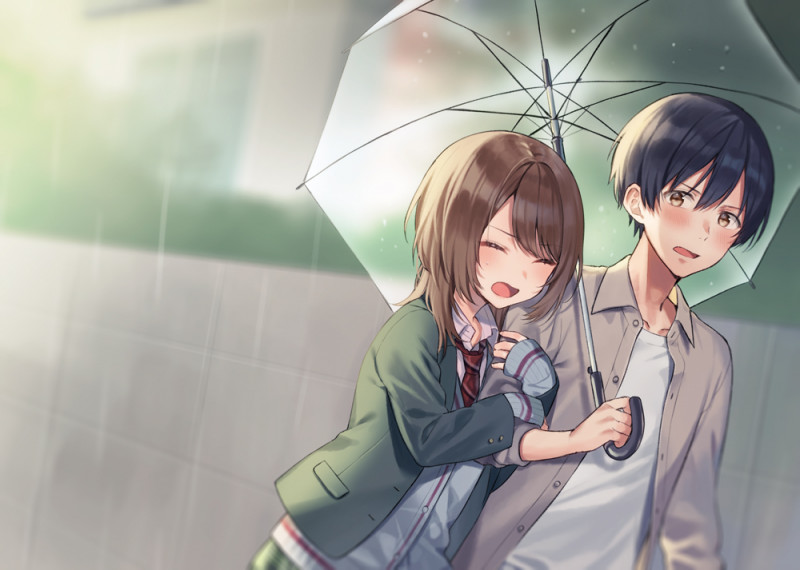
\includegraphics[width=\textwidth]{assets/u6440-7332b46f-e0f7-4bd4-9b9e-b153d3bf1de5.jpg}
\end{center}
\\
“N-, nó vừa đánh xuống đúng chứ!? Đánh xuống ngay gần đây luôn đúng chứ!? Ở đâu thế……”\\
“Tớ có biết đâu……nhưng mà cậu làm ơn buông tớ ra được không?”\\
“A~, xin lỗi……cậu không bị đau chứ?”\\
“Không có gì.”\\
\\
Để không cho cô ta biết mình dao động thì tôi cố làm thái độ hững hờ, nhưng rõ là con tim lại đang loạn nhịp.\\
Đã bao lâu rồi mới được Yuzuka ôm chầm lấy nhỉ? Tôi lơ đễnh cho thấy cái phản ứng chẳng giống với một thằng con trai đang trong tuổi dậy thì mất, nhưng do Yuzuka đang khá là dao động nên tôi chẳng hề bị nghi ngờ.\\
Bỏ chuyện đó qua một bên đã.\\
Thế này thì xong xuôi một vụ.\\
Sau đó đưa cho Yuzuka chiếc dù để cô ta quay trở về là được.\\
Chuyện đó hẳn là chắc chắn rồi, nhưng mà……\\
\\
“Nè, nè~, tớ ở nhà cậu một lúc được chứ?”\\
“T-, tại sao?”\\
“Vì tớ sợ sét lắm……không được sao?”\\
“……Ừ thì, nếu là trú mưa thì được thôi.”\\
Không thể bỏ rơi gương mặt sắp chực khóc đó của Yuzuka, sau khi kiểm tra không có ai trong nhà rồi thì chúng tôi bước vào.\\
-OoO-\\
Đọc bản dịch gốc và ủng hộ nhóm dịch tại \href{https://ln.hako.re/}{ln.hako.re}\\
\newpage

    \begin{center}
    \textbf{\large Chương 05 \\ Tuy khó chịu, nhưng mà đã rất vui}
    \end{center}
    \noindent
Mời vợ cũ vào phòng đã là tệ rồi, mà bị gia đình trông thấy thì còn tệ hơn nữa, thành thử tôi chỉ còn nước để cho Yuzuka vào phòng mà thôi.\\
Rồi thì Yuzuka làm vẻ mặt trông như khó xử.\\
Cô ta đang xấu hổ khi ghé thăm phòng của con trai——à đương nhiên là không phải thế rồi.\\
Ánh nhìn ấy đang được hướng đến mấy con figure.\\
\\
“Cái này……”\\
“À, àà, cái đó à. Là con figure đầu tiên trong đời tớ lấy được đó.”\\
\\
Nhìn thấy nó ở trung tâm trò chơi, nhẹ dạ rớ tay đến thì những tờ tiền 1000 yên lần lượt bay đi, để rồi cuối cùng tôi tiêu gần 5000 yên vào đấy.\\
Lúc lấy được nó trong tay thì cảm giác thật là tuyệt vời, lúc nó bị hỏng thì cảm giác mất mát cũng thật là kinh khủng.\\
Tôi đã trân quý nó rồi, vậy mà Yuzuka lại ném nó đi lúc vợ chồng cãi nhau, khiến nó đập vào tường và hư hỏng.\\
Lúc đó tôi thật sự đã tức giận.\\
Nhìn thấy con figure thì ký ức chẳng mong muốn ấy lại vực dậy.\\
\\
“Cậu chơi game không?”\\
“Được chứ?”\\
“Không làm gì thì chán lắm.”\\
\\
Nếu chơi game sẽ khiến phân tâm, không làm mấy cái hành động khả nghi là xong.\\
Tôi đưa cô ta bộ điều khiển và chọn phần mềm.\\
\\
“Game đối kháng với co-op, cậu thấy cái nào được?”\\
“Tớ thích coop. Kurose-kun thì sao?”\\
“Tớ có lẽ cũng thích co-op.”\\
\\
Tôi thì chẳng hình dung ra cảnh tượng có thể co-op được với Yuzuka, nhưng có khả năng nếu chơi đối kháng sẽ cãi nhau mất.\\
Chính vì thế mà tôi chọn trò Tam Quốc vô song$^\text{[note43540]}$ và bắt đầu chơi.\\
Khi đoạn movie chiếu thì Yuzuka vui vẻ hớn hở.\\
\\
“Ưwa~, hoài niệm quá!”\\
“Có hoài niệm đến mức nói thế không đó? Tớ nghĩ nó mới được phát hành vào kỳ nghỉ xuân thôi mà……”\\
“P-, phải rồi ha. Tớ nhầm với game khác mất rồi! Vậy tức là cậu chưa nuôi nhân vật nào ha?”\\
“Chỉ những nhân vật mà tớ thích đã max status hết cả rồi.”\\
“Đâu nào……Ưwa~, thật luôn. Toàn những nhân vật nữ quyến rũ nhỉ.”\\
“C-, có sao đâu. Tớ thấy vui khi di chuyển mấy nhân vật nữ hơn.”\\
“Nhưng chẳng phải mấy nhân vật nam có nhiều kỹ năng ngầu hơn sao?”\\
“Bên mấy nhân vật nữ có dàn seiyuu hào hoa còn gì.”\\
“Vậy cậu thích nhân vật nào?”\\
“Tớ thích nhân vật này.”\\
“Là Idol seiyuu ha. Cậu đừng có thích người ta quá sẽ tốt hơn. Khi người ta kết hôn rồi cậu sẽ sốc rồi liệt giường vài ngày cho mà xem.”\\
“Ừ, ừ thì nếu như cô ấy kết hôn thì tớ có lẽ sẽ nằm liệt giường thật……”\\
\\
Thực tế thì, tôi đã ốm liệt giường.\\
Được Yuzuka chăm sóc, và khi nói ra sự thật thì được cô ấy làm cho cái biểu hiện cạn lời.\\
Nói chung là, tôi muốn cô ta đừng nói ra cái từ ‘kết hôn’. Vì hiện tại nó rất là nhạy cảm đấy.\\
\\
“Độ khó thì chọn thế nào?”\\
“Chỉ có một sự lựa chọn là khó thôi. Cùng hội quân sau khi hạ gục hai con tướng nhé.”\\
“Ôkê.”\\
\\
Chúng tôi điều khiển tướng, trảm gục từng quân địch.\\
Do chọn độ khó cao nhất nên địch rất thông minh, nhưng đây là game mà tôi đã chơi từ xưa rồi. Với sức mạnh ‘nhất kỵ đương thiên’$^\text{[note43539]}$ mà tôi áp đảo toàn bộ quân địch, hội ngộ với Yuzuka rồi chiến cục cứ thay đổi sang cứu và được cứu lấy nhau.\\
Tuy là đồ họa có thô, nhưng cả hai cùng chơi thì lại rất vui.\\
Thế này thì làm tôi nhớ lại cuộc sống vợ chồng đã từng vui vẻ.\\
Mối quan hệ vợ chồng lạnh nhạt đi rồi tôi đã hoàn toàn quen với game trên mạng xã hội, nhưng lúc còn hòa thuận, mỗi ngày hai vợ chồng đều chơi game như thế này cho đến tối nhỉ.\\
Vậy mà do lão giám đốc chết tiệt mà công ty bị phá sản. Tôi chẳng còn dư dả thời gian để chơi game, rồi mối quan hệ vợ chồng trở nên lạnh nhạt đi.\\
Tuy là tôi chẳng có lấy một chút mong muốn nối lại tình xưa với Yuzuka, nhưng tôi sẽ đi xin việc tại một công ty khác ở đường thế giới này cho xem.\\
\\
“Hoan hô! Clear rồi!”\\
“Thắng dễ ghê ha.”\\
“Tớ hạ được 5 con tướng đó. Còn cậu thì sao?”\\
“Tớ cũng thế.”\\
“Nếu vậy thì, tớ thắng nhé.”\\
“Hả? Tại sao lại như thế?”\\
“Vì nhân vật của tớ chưa được nuôi mà.”\\
“Nhân vật đó vốn dĩ từ đầu status đã cao rồi mà. Với status hiện tại thì dù là nhân vật của tớ cũng sẽ có sức mạnh cỡ đó còn gì.”\\
\\
Chúng tôi nói với nhau như thế, nhưng cái này chẳng phải là cãi nhau.\\
Nói với nhau cỡ này như là chuyện cơm bữa, là bằng chứng nổi hứng khi chơi game ấy mà. Lúc quan hệ vợ chồng trở nên lạnh nhạt rồi thì chỉ toàn tặc lưỡi chẳng nói lời nào thôi.\\
\\
“Lần tới tớ sẽ hạ nhiều hơn Koikawa-san cho xem.”\\
“Tớ sẽ hạ hết tất cả cho cậu thấy.”\\
\\
Cầm chặt bộ điều khiển trên đôi tay đã đẫm mồ hôi, chúng tôi tiến đến màn tiếp theo—\\
\\
“Nii-chan Nii-chan!”\\
\\
Ư ô~!\\
Con em Sana về mất rồi!\\
Nó đang chạy rầm rầm lên tầng trên, và đang tiến thẳng đến đây!\\
\\
“Koikawa-san, trốn đi!”\\
“Ể~? T-, tại sao?”\\
“Nếu bị con em gái thấy sẽ gặp nhiều phiền toái lắm!”\\
\\
Một thằng anh chán ngắt dẫn con gái về khi mới chỉ nhập học thì nó sẽ đến quấn lấy tôi một cách khó chịu cho xem.\\
Với lại Yuzuka và Sana hợp tính một cách kinh khủng. Cô ta sẽ bắt đầu đến nhà dù cho tôi từ chối, được gia đình tôi công nhận, và có lẽ sẽ hướng theo lộ tình yêu đương không chừng.\\
Thậm chí còn liên quan đến nhau hơn những gì mà tôi đã tưởng tượng nữa. Tôi muốn tránh cái bước tiến triển này thêm cơ.\\
\\
“Nguy rồi nguy rồi! Nguy rồi Nii-chan!”\\
\\
Chuyện Sana đến phòng và Yuzuka trốn ở giường xảy ra gần như là đồng thời với nhau.\\
\\
“G-, gì thế? Mà vào thì phải gõ cửa chứ.”\\
“Có mà, bên trong tâm trí em này.”\\
“Mẹ vào mà chẳng thèm gõ luôn ấy……Rồi thì, cái gì nguy hả.”\\
“Anh nhìn cái này đi!”\\
\\
Sana đến cho tôi xem cái điện thoại.\\
Trên màn hình hiển thị hình ảnh mái nhà của nơi nghỉ chân đã bị phá hủy.\\
\\
“Chỗ nghỉ chân của công viên bị sét đánh! Em nhận được tin nhắn từ Micchan đó!”\\
“Thế à.”\\
“Phản ứng của anh nhạt thật đó Nii-chan!”\\
“Anh đang mệt do chơi game đây.”\\
“Thế à. Mình ra công viên xem đi anh!”\\
“Anh đã nói là đang mệt rồi mà……Sau khi tạnh mưa rồi đi nên là ra ngoài giùm anh cái.”\\
“Đã rõ~!”\\
\\
Nói bằng giọng tràn đầy sức mạnh rồi thì Sana đi khỏi.\\
Và Yuzuka thò mặt ra từ chiếc giường.\\
\\
“Em gái cậu khỏe khoắn thật ha.”\\
“Nhờ thế mà mỗi ngày tớ đều mệt đấy.”\\
“Thế à? Trông như cậu sẽ nhận lấy năng lượng khỏe khoắn mà.”\\
\\
Một con nhỏ Sana hệ xà nẹo đối với Yuzuka, một đứa có xu hướng tạo khoảng cách với người khác, là một sự tồn tại đáng quý.\\
Sana dường như cũng giỏi lắng nghe nữa, có vẻ như nó thường được nghe những lời phàn nàn về tôi từ Yuzuka. Nếu như Sana không nghe những lời phàn nàn thì stress của Yuzuka sẽ không mất đi, và có lẽ chuyện ly hôn sẽ diễn ra sớm hơn rồi chăng.\\
Dù sao đi nữa, không gặp mặt nhau khiến tôi tạm thời an tâm rồi. Nếu như gặp nhau thì có khả năng sẽ thân với nhau tại đây luôn quá.\\
\\
“Vậy rồi, tớ nên làm thế nào mới được?”\\
“Lúc nào quay về từ câu lạc bộ nó đều đi tắm cả, nên hãy ra về lúc ấy giúp tớ.”\\
\\
Đột nhiên cánh cửa được mở ra.\\
\\
“Phải rồi Nii-chan! Ở ngoài cửa có đôi giày mà em nhìn không quen lắm——Ưhyaaa~!? Nii-chan dẫn gái về nhà! Đồ ecchi!”\\
“Ecchi quái gì! Mà mẹ trẻ biết gõ cửa không thế?”\\
“Em có mà!”\\
“Lại ở trong tâm trí chứ gì!”\\
“Nếu như anh nghe thấy rồi thì có vấn đề gì đâu.”\\
“Nghe thấy thế qué nào được! Nii-chan bận lắm nên đi ra đằng đó đi! Với lại, giữ bí mật với mẹ chuyện này n—”\\
“Kouhei~! Ở ngoài cửa có đôi giày của con gái này, con dẫn về nhà đó hả~!? Giới thiệu cho mẹ xem nào~!”\\
Và rồi tôi chỉ muốn ôm đầu vì mẹ lại về nhà đúng cái lúc tồi tệ nhất mà thôi.\\
-OoO-\\
Đọc bản dịch gốc và ủng hộ nhóm dịch tại \href{https://ln.hako.re/}{ln.hako.re}\\
\newpage

    \begin{center}
    \textbf{\large Chương 06 \\ Thế là cả hai nắm rõ chuyện xuyên không}
    \end{center}
    \noindent
Chuyện ngay sau khi chúng tôi bị Sana và mẹ bắt quả tang tại trận.\\
Bọn tôi đã di chuyển đến phòng ăn. Và hiện tại thì thằng này đang vừa uống hồng trà, vừa khổ sở nhìn 3 người họ nói cười rôm rả.\\
Cái khung cảnh mẹ, em gái và vợ cũ nói chuyện làm tôi đau tim cực kỳ. Vậy mà có thể thấy Yuzuka đang trông rất ư là dễ chịu.\\
Dù là ở đường thế giới trước thì lúc gặp cô ta đã cởi mở này, thân thiết đến mức hơn cả so với gia đình mình luôn ấy chứ.\\
Ngược lại thì tôi lại chẳng hòa thuận với ba mẹ của Yuzuka. Nếu như tính cách của ba mẹ bên ấy giống với lại ba mẹ tôi thì có lẽ cuộc sống hôn nhân cũng đã kéo dài rồi.\\
\\
“Koikawa-chan, cháu uống thêm hồng trà chứ?”\\
“Cảm ơn bác nhiều ạ. Cháu xin nhận.”\\
“Nè~ nè~! Koikawa-san quen biết với lại Nii-chan nhà em ở đâu thế?”\\
“Đương nhiên là ở trường rồi.”\\
“Đằng nào mở chuyện trước ạ?”\\
“Là từ chị. Chị gặp anh ấy ở hiệu sách, sau đó còn cho chị mượn dù ở công viên nữa.”\\
“Nii-chan được ghê~! Thế ra anh cũng có can đảm để đi tán gái này nọ ha!”\\
“Tán gái cái gì mà tán gái. Là quan tâm đơn thuần thôi.”\\
“Vả lại còn đột nhiên cho chị ấy ngủ trên giường nữa chứ~! Mới ngày đầu nhập học cao trung mà đã thế này rồi~! Nii-chan đột nhiên bắt đầu tận hưởng thanh xuân, làm em gái như em đây nào là mừng, nào là cô đơn đó!”\\
\\
Sana nói thế, rồi nở nụ cười toe toét làm tôi chẳng cảm nhận được tí nào sự cô đơn của mẹ trẻ. Em ấy học trung học năm 2 thì hẳn đang thèm khát mấy chuyện tình yêu rồi. Đã thế chuyện tình yêu của người thân bất chợt nảy nở càng khiến cho con bé rất ư là háo hức.\\
\\
“Nhưng mà đã hiếm có dịp ở cùng với con gái rồi mà anh lại mời chị ấy về để chơi game nữa. Làm chuyện gì đó lãng mạn hơn đi.”\\
“Có sao đâu. Koikawa-san có sở thích với game mà.”\\
“Thật vậy ạ?”\\
“Ừm. Chị thích game mà. Chơi game cùng với Kurose-kun thú vị lắm.”\\
“Siêu hợp tính luôn kìa!”\\
“Còn quá sớm để bảo là siêu hợp tính đấy. Anh mới gặp chị ấy ngày hôm nay thôi.”\\
\\
Ngày xưa thì tôi cũng đã từng nghĩ rằng chúng tôi siêu hợp tính, nhưng nếu thế thì đã chẳng ly hôn rồi.\\
\\
“Koikawa-san, chị nghĩ thế nào về Nii-chan? Chị có chút hứng thú với anh ấy đúng chứ?”\\
“Oi, đừng có hỏi mấy câu khiến người ta khó trả lời chứ. Koikawa-san cũng không thích bị hỏi thế đâu đúng không. Con em gái này để tớ dạy dỗ nó sau, cậu nên về trước khi bị hỏi mấy câu kỳ cục sẽ tốt hơn đấy.”\\
“Ư, ừm. Tớ thì ngoại hình tuy có chút đáng sợ, nhưng lại thấy cảm thấy dễ chịu khi được người như Sana-chan dính chặt lấy đó.”\\
“Nghe gì chưa Nii-chan? Chị ấy nói thích mấy bé như em đó! Em vui quá cơ~. Chị tốt đến nỗi thật là lãng phí khi sánh vai với Nii-chan đó!”\\
“Tuy lúc nào cũng dối lòng nhưng bản chất là một đứa tốt bụng, nên từ giờ cháu hãy hòa thuận với lại Kouhei nhà bác nhé?”\\
“Dạ. Nếu như Kurose-kun thấy ổn ạ……”\\
“Tất nhiên là được rồi chứ chị!”\\
\\
Oi oi, đừng có tự tiện mà lấn tới coi.\\
Tôi không có ý muốn hòa thuận với con nhỏ này đâu.\\
Tôi muốn nói thế, nhưng miệng thì lại chẳng thể mở ra. Vì nếu như tôi nói thì sẽ bị họ truy cùng đuổi tận lý do cho xem. Có mắc sai lầm đi nữa cũng không thể nói ra chuyện đã xuyên không về được.\\
\\
“A~, phải rồi phải rồi. Nhân tiện thì tên của chị là gì thế, Koikawa-san?”\\
“Là Yuzuka.”\\
“……Yuzuka?”\\
“Có gì lạ sao?”\\
“Ư ừn. Cực kỳ dễ thương ạ. Chỉ là cái tên$\lfloor$Yuzuka$\rceil$em có cảm giác đã nghe ở đâu rồi……Đúng rồi! Là vợ của Nii-chan!”\\
\\
Thế quái nào lại biết thế hả!?\\
Chẳng lẽ đây cũng là cuộc đời thứ 2 của em à!? Em cũng đến từ đường thế giới mà anh và Yuzuka đã ly hôn á!?\\
Khi mà tôi vẫn giữ nguyên cái bộ mặt tỉnh bơ thì Yuzuka chớp mắt ngạc nhiên.\\
\\
“E, eeto……Vợ tức là sao em?”\\
“Cậu không cần phải nghiêm túc hiểu đâu. Nó chỉ đang đùa giỡn thôi!”\\
“Em có đùa giỡn gì đâu. Chẳng phải buổi sáng Nii-chan đã nói sao. Nào là Yuzuka có vô sự không, nào là vợ rồi vợ cũ nữa. Tuy là anh nói mới gặp hôm nay, nhưng thật ra là đã gặp chị ấy hôm đi xem điểm thi rồi đúng không nè!”\\
“Mẹ cũng đi cùng vậy mà hoàn toàn chẳng nhận ra luôn~!”\\
“Hèn chi ảnh chẳng chịu dậy. Ra là đã mơ thấy giấc mơ hạnh phúc hen.”\\
\\
Sana và mẹ tôi mỉm cười trông thích thú, nhưng Yuzuka thì lại trông khá khó xử. Gò má của cô ta co giật, rồi loáng thoáng nhìn về phía tôi.\\
Thế này thì tệ rồi. Cực kỳ tồi tệ luôn!\\
Nếu cứ thế này thì chuyện tôi đích thực xuyên không về sẽ bị bại lộ mất!\\
\\
“Ngủ mơ thôi mà! Mà hơn hết thì đói bụng quá! Con trưa giờ chưa ăn gì hết đó!”\\
“Cháu ăn gì chưa Koikawa-chan?”\\
“Dạ, vẫn chưa ạ……”\\
“Thế thì gọi sushi đi, sushi đi mẹ!”\\
“Phải ha. Cũng là ngày kỷ niệm mà, cùng ăn mừng thôi!”\\
“A, không ạ, cháu nghĩ cũng sắp đến lúc phải về rồi……”\\
“Được mà, chị không cần phải ngại đâu chu!”\\
“Cháu cứ xem đây là nhà mình là được rồi!”\\
\\
Bị hai người họ níu giữ lại, Yuzuka chỉ còn biết nhếch đôi gò má lên và cười thôi.\\
Bộ dạng đang muốn rời khỏi đây đấy, nhưng có vẻ như không thể từ chối hảo ý từ Sana và mẹ mà cô ta yêu quý.\\
\\
“Nhắc mới nhớ, Koikawa-san, chẳng phải cậu nói là có việc sao?”\\
“P-, phải phải. Đúng là tớ có việc!”\\
“Thế sao~. Em muốn nói chuyện thêm một chút với chị, vậy mà tiếc quá. Nhà của chị gần đây chứ, Koikawa-san?”\\
“Là khu căn hộ ở gần đây thôi……”\\
“Vậy thì Nii-chan đưa chị ấy về đi!”\\
“T-, tại sao lại là anh……Koikawa-san muốn về một mình còn gì.”\\
“Ư ừn. Nếu như cậu có thể đưa tớ về thì tớ muốn cậu làm thế cơ.”\\
\\
Bên phía mẹ thì đang híp đôi mắt lại cười toe toét khi thấy Yuzuka chẳng hiểu sao mà trở nên háo hức.\\
Bọn họ nói 1 câu dư thừa ‘có về trễ một chút cũng không sao đâu’ rồi tiễn chúng tôi.\\
Dưới cơn mưa nhỏ, mỗi đứa cầm chiếc dù mà bước đi trong yên lặng.\\
Không thể chịu đựng được sự yên tĩnh khó xử hay sao mà Yuzuka đã là người lên tiếng trước.\\
\\
“Nè, nè~ Kurose-kun?”\\
Cô ta gọi tôi là$\lfloor$Kurose-kun$\rceil$, tiếc là vẫn chưa có bằng chứng nhỉ?\\
Nếu thế thì tôi sẽ đánh trống lảng cho xem!\\
\\
“G-, gì thế?”\\
“Thì……chuyện mà Sana-chan nói ban nãy, là thật chứ?”\\
“A, àà, chuyện đó à. Tối qua tớ thức trắng để chơi galgame đấy. Tình cờ là đang theo tuyến của nhân vật tên là Yuzuka ấy mà. Rồi, tớ tình cờ mơ thấy giấc mơ kết hôn. Thế nên là hoàn toàn chẳng liên quan gì đến Koikawa-san đâu.”\\
“……Love Minus.”\\
\\
Yuzuka lẩm bẩm nói ra.\\
\\
“Love Minus……?”\\
“Là game mô phỏng tình ái được phát hành vào mùa xuân này đó.”\\
“Cái đó thì tớ biết, nhưng tại sao đột nhiên lại nói về Love Minus? A, có lẽ nào Koikawa-san cũng có hứng thú với Love Minus sao?”\\
“Tớ chẳng có hứng thú đâu. Chỉ là, tớ biết nó là game như thế nào thôi. Vì ngày xưa đã từng có người nói cho tớ biết. Rằng, đó là trò chơi chính là bản thân sẽ hòa thuận với ai đó trong số senpai, bạn cùng lớp, hay là kouhai, tỏ tình, tận hưởng buổi hẹn hò, rồi sau đó trở thành người yêu của nhau.”\\
“Cậu biết rõ ghê ha.”\\
“Phải. Tớ biết rõ lắm. Trong số 3 người không có nhân vật nào tên là Yuzuka cả.”\\
“Thì trò đó làm gì có nhân vật nào tên là Yuzuka, nhưng cái tớ chơi hôm qua là trò khác cơ.”\\
“Chẳng phải đã nói về game tình ái chỉ chơi mỗi trò Love Minus thôi nhỉ?”\\
“Ai nói?”\\
“Là anh đó!”\\
“Đ-, đừng có đột nhiên hét lên chứ. Cơ mà……Ể? Cậu làm sao thế Koikawa-san? Giống như là biến thành người khác vậy ấy.”\\
“Mặt dày thật đấy! Anh cũng thế mà đúng chứ!? Xuyên không ấy!”\\
\\
Bước vào trong chiếc dù của tôi, nắm lấy vai như là để tôi không thể bỏ chạy rồi Yuzuka nổi giận hét lên.\\
……Bị bại lộ hoàn toàn rồi ha.\\
Nếu là thế thì thành thật làm rõ sẽ tốt hơn. Làm như thế rồi thì chẳng lần nào nữa vướng bận với nhau là xong.\\
\\
“Nếu thế thì sao hả.”\\
\\
Khi tôi quay ngoắt lại thừa nhận thì Yuzuka lườm đến.\\
Cô ta run bần bật, gương mặt xấu hổ đã nhuộm đỏ.\\
\\
“Thế tại sao anh lại lừa hả! Muốn trông thấy tôi cố gắng diễn vai nữ sinh cao trung rồi cười chế giễu trong lòng đúng chứ!”\\
“Ai lại đi làm cái chuyện tồi tệ đấy hả~! Cả tôi cũng đang bối rối về chuyện xuyên không đây! Chẳng có thời gian để quan sát thân hình cô trong bộ đồng phục đó đâu! Thêm vào đấy là cái đứa vợ cũ lại đến lại vướng mắc với bản thân nữa! Chẳng phải là cô chẳng muốn liên quan gì đến tôi à!”\\
“Tôi có đến để vướng mắc gì với anh đâu! Tại sao anh lại không lập tức làm rõ hả!?”\\
“Tôi đang chờ thời cơ đến thôi! Tôi thì cả một ngày hôm nay đã khổ tâm lao lực lắm đấy. Do cô đột nhiên nói mình là Kurose Yuzuka nên tôi đã phải vất vả diễn trò để không bị lộ ra đấy!”\\
“Quả nhiên anh đã nghe từ lúc giới thiệu bản thân! Cái gì mà ngủ không đủ chứ! Chẳng phải làm tôi có chút lo lắng cho anh à!”\\
“Ngủ không đủ là thật đấy! Mỗi ngày tôi phải làm việc đến tối muộn! Cô thì tốt rồi, cứ chiều là được về!”\\
“Lại nói chuyện đó nữa hả!? Lỗi chẳng phải do anh không nhận việc tại một công ty đàng hoàng à!”\\
“Lần tới tôi sẽ làm việc tại một công ty đàng hoàng cho coi! Rồi sau đó sẽ tận hưởng cuộc sống độc thân!”\\
“Tôi cũng sẽ không kết hôn lần nữa đâu! Nhất là với anh đấy!”\\
“Tất nhiên rồi! Có nhìn thấy nhau trong tiệm sách thì đừng có mà đến bắt chuyện lần nữa đấy!”\\
“Cả anh nữa, đừng có thấy tôi ở công viên rồi đến bắt chuyện lần nữa đấy!”\\
“Nếu như không biết trước chuyện sét sẽ đánh xuống công viên thì còn khướt tôi đến bắt chuyện với cô!”\\
“A-, anh muốn nói là đã cứu tôi đấy hả?”\\
“Phải đấy! Biết ơn một chút giùm cái đê!”\\
“Anh ghét tôi, thế tại sao lại đi cứu tôi hả?”\\
“Có phải tôi lo lắng cho cô hay gì đâu. Nếu gần nhà có người chết thì tôi sẽ cắn rứt lương tâm lắm. Cô cứ ở mãi trong công viên không chịu ra, nên suýt kéo cả tôi chết cùng đấy.”\\
“Nếu thế thì tại sao anh lại cứu tôi khỏi chiếc xe hả! Nếu như anh không đến xông vào tôi thì chỉ có mỗi một mình tôi chết vậy mà!”\\
“C-, có phải tôi đã cứu cô đâu……Chỉ tình cờ cô đứng trên đường tôi đi tới thôi!”\\
“Chẳng phải anh nói sẽ ngủ qua đêm tại tiệm nét cà phê à!”\\
“Tôi đổi ý thôi! Cơ mà nếu tự nhận thức được chuyện mình được cứu thì cảm tạ tôi đi chứ!”\\
“Chính xác mà nói thì anh không có cứu tôi! Không phải do bị xe đụng nên mới xuyên không về à!”\\
“Cũng đâu hẳn nguyên nhân là do bị xe đụng đâu chứ!”\\
“Cái hiện tượng siêu thường này chẳng phải định sẵn là do xe hơi hay xe tải tông trúng à!”\\
“Cô đừng đặt hiện thực với ảo tưởng chung một chỗ giùm cái!”\\
“Thế tại sao xuyên không về chứ hả!”\\
“Tôi biết thế quái nào được! Vốn dĩ nó không phải là xuyên không, mà chỉ là giấc mơ cũng không chừng!”\\
“Đừng có tự tiện bước vào trong giấc mơ của tôi cái!”\\
“Câu đó tôi nói mới đúng! Đừng có mà dính dáng đến cuộc đời của tôi~! Tôi đã quyết định sẽ sống mà chẳng dính líu đến cô ở đường thế giới này rồi!”\\
“Cả anh cũng đừng có mà dính dáng đến cuộc sống của tôi đấy!”\\
“Tất nhiên rồi! Đây là cuộc nói chuyện cuối cùng. Hứa là chẳng liên can gì đến nhau nữa đi!”\\
“Đấy là nếu anh chịu hứa!”\\
“Thế quyết định nhể! Đừng có khóc chỉ vì không có bạn đấy!”\\
“Anh cũng thế, đừng có mà ra vẻ thân mật chỉ vì không đào hoa đấy!”\\
\\
Những chùm pháo hoa nổ lộp bộp, rồi chúng tôi quay lưng lại với nhau, và cùng hứa sẽ không liên quan gì đến nhau nữa.\\
……Chắc chắn đã như thế rồi.\\
-OoO-\\
Đọc bản dịch gốc và ủng hộ nhóm dịch tại \href{https://ln.hako.re/}{ln.hako.re}\\
\newpage

    \begin{center}
    \textbf{\large Chương 07 \\ Chẳng thể nào dừng cãi yêu được}
    \end{center}
    \noindent
Ngày đầu tiên đến trường sau lễ nhập học.\\
Thấy tôi dậy sớm, mẹ nhìn với vẻ mặt ngạc nhiên.\\
\\
“Ara, hiếm khi mới thấy Kouhei dậy sớm hơn Sana như thế này đấy.”\\
“Có sao đâu. Tất nhiên con phải dậy sớm để đi học rồi.”\\
“Nói thế thôi, chứ thật ra không phải đã hứa đi học cùng với Koikawa-chan à?”\\
“Không có chuyện thế đâu mà~!”\\
\\
Ngược lại thì có.\\
Tôi dậy sớm là để không dính dáng gì đến cô ta.\\
Tôi cũng như Yuzuka mỗi ngày đều gần như trễ học.\\
Về chuyện mà sau này tôi nghe thì do nấu nướng$\cdot$giặt giũ$\cdot$dọn dẹp mất kha khá thời gian, lúc hoàn thành thì gần như là trễ học.\\
Tức là nếu đi học sớm thì tôi sẽ không chạm mặt với lại Yuzuka ở chỗ để giày.\\
Mới đây do hưng phấn mà tôi nằm mơ thấy chơi game cùng với Yuzuka, nhưng nếu cố tránh mặt nhất có thể thì chắc chắn cô ta sẽ không còn trong giấc mơ của tôi nữa.\\
Khi mà tôi đang ăn sáng thì Sana vừa dụi mặt, vừa đi đến.\\
\\
“Chào buổi sáng~……”\\
“Chào buổi sáng.”\\
“……Con nhìn thấy ảo giác Nii-chan này.”\\
“Thực thể đấy mẹ trẻ.”\\
“Hiếm khi mới thấy Nii-chan dậy sớm như thế này đó. Anh có hẹn với lại Koikawa-san ạ?”\\
“Đã bảo là không phải mà……”\\
\\
Tuy nói thế, nếu mà đi học trễ thì sẽ giống như là chờ hẹn gặp cô ta ở tủ để giày vậy.\\
Tôi ăn cho nhanh, điều chỉnh lại quần áo cho chỉnh tề rồi thì ra khỏi nhà sớm hơn dự định.\\
Bước đi trên con đường đến trường ít người, dưới một bầu trời thật xanh.\\
Nhiệm vụ của học sinh đến sớm nhất là mở cửa phòng học. Đương nhiên là tôi đến phòng giáo viên thử vì có thể bản thân mình là người đến sớm nhất, nhưng lại chẳng có chìa khóa của năm nhất lớp 1 đâu cả.\\
Có người đến sớm như thế này à. Một đứa học sinh đáng khâm phục thật ha.\\
Khi tôi vừa nghĩ như thế, vừa bước vào lớp học thì—\\
\\
“……Ge”\\
“……Hả?”\\
\\
Trong lớp học đã có một nữ sinh.\\
Chính là Yuzuka.\\
Trước hết thì cô ta đặt cặp của mình xuống ghế, rồi tặc lưỡi.\\
\\
“Do mơ thấy anh mà tôi thấy ảo giác của anh luôn đây này.”\\
“Tiếc thật nhể. Là thực thể hẳn hoi nhé.”\\
“Tại sao anh lại dậy sớm thế hả. Cái bản tính lúc nào cũng trễ học vậy mà.”\\
“Tôi không có trễ. Là gần trễ. Còn cô hôm nay không làm việc nhà mà đến trường à?”\\
“Tôi đã làm đàng hoàng rồi. Lúc xưa tuy có tốn thời gian, nhưng nhờ ai đó đùn đẩy việc nhà một mình cho tôi mà thành ra đã quen tay mất rồi.”\\
“Tôi có đùn đẩy một mình đâu. Mỗi lần đều do tôi đi vứt rác đấy thôi.”\\
“Anh đã nói$\lfloor$cứ để mấy việc tốn sức cho anh$\rceil$mà đúng chứ. Đừng có mà tự hào cái chuyện đi vứt rác giùm tôi cái.”\\
“Nhưng mà cô mỗi lần đều đến hôn tôi và nói$\lfloor$thưởng cho anh nè$\rceil$à.”\\
“L-, lúc đó tôi bị sao sao đấy thôi~! Đại khái thì cái bên nói$\lfloor$nhớ chuẩn bị nụ hôn cho anh nhé$\rceil$mới là bên có lỗi à.”\\
“T-, thì nếu như cô không muốn hôn thì không phải hôn cũng được còn gì~! Đã hôn tôi bằng ý nghĩ của bản thân thì đừng có mà phàn nàn với tôi giùm cái!”\\
“Nếu không hôn thì anh sẽ dỗi còn gì!”\\
“Tôi không có dỗi!”\\
“Anh có dỗi!”\\
“Dỗi cái khỉ khô! Có bao giờ tôi không được hôn sau khi đi vứt rác đâu! Làm gì có lý do để mà hờn dỗi chớ!”\\
“Cũng có lúc chưa hôn kia mà!”\\
“Là lúc nào!”\\
“Lúc tôi bị ốm đó!”\\
“Nếu cô bị ốm thì đương nhiên tôi sẽ đi vứt rác, mà cô đang ốm thì làm sao tôi có thể mở miệng đòi thưởng được chứ! Nói chung là không tính! Cơ mà không chỉ đi vứt rác, tôi cũng có dọn dẹp rồi còn gì.”\\
“Dọn dẹp á, chẳng phải anh chỉ làm mỗi ngày nghỉ thôi à.”\\
“Thì do cô nói$\lfloor$anh Kouhei đi làm trễ hơn nên việc dọn dẹp cứ để em lo$\rceil$mà. Tôi vào ngày nghỉ có dọn dẹp đàng hoàng vẫn giữ gìn sạch sẽ đó thôi.”\\
“Cái đó thì thì do anh đã nói với tôi là$\lfloor$dọn dẹp thì anh sẽ làm cẩn thận vào ngày nghỉ, nên em chỉ cần dùng máy hút bụi qua loa cũng được$\rceil$đấy!”\\
“Dù có thế nào đi nữa có quá là qua loa rồi còn gì! Cuộn băng keo sau khi tôi lăn dính đầy tóc đấy!”\\
“Chẳng phải là tóc của anh à!”\\
“Toàn bộ có phải là tóc của tôi đâu!”\\
“90% là của anh đấy! Không phải anh nói$\lfloor$dạo gần đây tóc anh rụng nhiều hơn$\rceil$rồi dùng thuốc mọc tóc à!”\\
“Cái đó thì có sao đâu! Đại khái tôi rụng tóc nhiều hơn cũng là do stress—nói chung là do cô mà ra đấy!”\\
“Nếu như anh stress khi ở cạnh với tôi đến thế thì đừng có dính dáng đến tôi chứ!”\\
“Là do cô bắt chuyện trước còn gì!”\\
“Lỗi do anh không đi trễ mới đúng chứ!”\\
“Cô đi trễ giùm cái đi!”\\
“Không thích. Nếu đi trễ thì tôi sẽ bị nghĩ mình là yankee mất.”\\
“Nếu thế thì làm cái gì đó với ngoại hình đi. Cô đeo kính áp tròng vào thì ánh mắt sẽ đỡ tệ hơn con gì.”\\
“Tôi tuyệt đối không muốn bỏ gì đó vào mắt đâu. Đáng sợ lắm.”\\
“Làm gì đáng sợ đến mức đó. Cơ mà không phải lúc trước tôi thực diễn để chứng minh cho cô thấy là không đau à. Lúc đó bộ nhìn tôi đau đớn lắm hả?”\\
“Không có. Nhưng mà nhìn với lại làm nó là hai chuyện khác nhau chứ.”\\
“Nếu thế thì đeo kính vào đê. Rồi làm cho tóc đen trở lại thì sao hả?”\\
“Đột nhiên thay đổi ngoại hình, cứ như thể là màn ra mắt cao trung thất bại vậy, chẳng phải xấu hổ lắm à.”\\
“Đằng nào đi nữa thì cái lộ trình này sẽ thất bại còn gì. Cô nên ăn năn một chút đi.”\\
“Tôi ăn năn nên mới đi học sớm đấy. Nghĩ rằng đi trên lộ trình đàng hoàng sẽ có người đến bắt chuyện với mình……”\\
“Bản thân cô đến bắt chuyện đi chứ.”\\
“Không thể nào. Ngượng quá ấy chứ.”\\
“Cho đến dạo trước cô còn làm nữ tiếp tân cho doanh nghiệp lớn vậy mà xấu hổ cái gì hả.”\\
“Tôi là loại người tách biệt công việc với chuyện cá nhân đấy. Cả cái lúc mà tôi nói chuyện với anh trên đại học, tôi đã cực kỳ lo lắng lắm đấy.”\\
“Tôi biết chứ. Cô bập bà bập bẹ luôn ha.”\\
“Chẳng phải cả anh cũng rụt rà rụt rè à.”\\
“Đột nhiên được một đứa con gái bập bà bập bẹ nói chuyện với mình thì đương nhiên tôi phải rụt rè rồi.”\\
“Thế nên anh mới chẳng đào hoa ha.”\\
“Đừng có nói tôi không đào hoa. Cơ mà tôi đã khác với tôi của lần trước rồi nhé. Tôi đã học cách trưng diện rồi đấy.”\\
“Làm gì mà ra vẻ thế. Anh nghĩ ai là người dạy anh cách trưng diện hả? Nếu như không có tôi thì bộ dạng của anh cũng đành giống với lại thời trung học dù ở trên đại học thôi.”\\
“Cô làm gì biết thời trung học của tôi chứ.”\\
“Tôi biết chứ. Vì mẹ anh cho tôi xem ảnh rồi.”\\
“Tôi đã bảo bả đừng cho xem đến thế rồi vậy mà……!”\\
“Anh mua cái găng lộ ngón đấy ở đâu thế?”\\
“Đừng có hỏi!”\\
“Gì đấy. Anh đâu cần phải cáu lên như thế!”\\
“Do cô làm nhục tôi còn gì!”\\
“Thế chẳng phải anh nhìn tấm hình thời trung học của tôi rồi cười toe toét đấy sao!”\\
“C-, cái đấy là tại tôi đã nghĩ cô dễ thương chứ không có xem thường cô gì hết!”\\
“Th-, thế thì lúc đó nói thẳng ra đi chứ! Tại sao bây giờ mới nói ra hả!?”\\
“Vì tôi nghĩ nếu khen bộ dạng cô lúc xưa kiểu gì cũng bị cô dỗi. Thực tế thì, cô đã dỗi rồi nói$\lfloor$ra là anh thích loại này$\rceil$khi mà tôi thích mấy nhân vật tóc đen trong anime à?”\\
“C-, cái đó thì còn cách nào khác đâu! Vì lúc đó tôi đã thích anh mà! Nhưng mà bây giờ thì khác! Anh cứ đi mà thích mấy nhân vật tóc đen hay nhân vật đeo kính gì đó thì tùy!”\\
“Cô bây giờ có nói ra cũng đã quá trễ rồi! Do cô mà tôi thích nhất mấy nhân vật tóc màu nâu và ánh mắt xấu tệ rồi đấy!”\\
“Đừng có mà đổ lỗi cho tôi!”\\
“Là do lỗi cô để tóc màu nâu với ánh mắt xấu tệ còn gì! ……Với lại lúc nãy cô nói$\lfloor$nhân vật tóc đen hay là nhân vật đeo kính$\rceil$ấy nhỉ?”\\
“Thì có nói.”\\
“Tại sao chỉ toàn giới hạn trong 2D thế hả!”\\
“Vì tôi chẳng nghĩ anh có thể yêu một ai đó 3D đâu!”\\
“Trước khi có thể hay không thể thì tôi chẳng còn có hứng thú để yêu đâu! C-, có lẽ tôi sẽ trở nên thân thiết với lại Hagakure-san không chừng.”\\
“Hagakure-san á, là cái người ít nói ấy ư?”\\
“Phải rồi đấy. Tôi lúc học năm nhất đã cùng với Hagakure-san làm ủy viên thư viện. Hagakure-san là một otaku ẩn nên tôi có thể trở nên thân thiết với nhỏ đấy.”\\
“Động thủ với nữ sinh cao trung à? Dính đến pháp lý rồi đấy.”\\
“B-, bây giờ bọn tôi cùng tuổi thì chẳng vấn đề gì còn gì~!”\\
“Chẳng phải bên trong là một ông chú à.”\\
“27 tuổi thì chú chiếc cái gì! Đại khái, nếu cô nói như thế thì cô cũng là một bà thím đang cosplay đồ nữ sinh cao trung đấy thôi.”\\
“Nếu như anh bận tâm thì đừng có mà nói đến~! Anh không cần nói tôi cũng biết là tôi chẳng hợp với bộ đồng phục mà……”\\
“Tôi có nói là không hợp đâu! Cơ mà nếu như cô xấu hổ thì làm gì với độ dài của cái váy đi! Bị ai đó thấy quần lót thì tính sao hả!”\\
“Với ngoại hình này mà mặc váy dài thì chẳng phải tôi sẽ như đầu gấu à. Cả anh cũng làm gì đó với đồng phục mình đi. Cả trên cả dưới đều rộng thùng thình. Tại sao lại mua độ rộng như thế hả?”\\
“Tôi đang nghĩ mình sẽ cao lên thôi.”\\
“Tiếc ghê ha. Anh vĩnh viễn cũng chẳng đạt tới 170cm đâu.”\\
“Nhớ đấy nhé. Mỗi ngày tôi sẽ uống sữa để thoát cảnh 169cm cho cô thấy!”\\
“Thế thì cố lên. Với lại anh cũng từ bỏ cái chuyện trở thành ủy viên thư viện đi. Tôi cũng đang nghĩ định trở thành ủy viên thư viện đây.”\\
“T-, tại sao lại thành ủy viên thư viện thế hả! Cô đi mà làm ủy viên thể dục giống với hồi năm nhất đi!”\\
“Tôi không muốn làm ủy viên thể dục nữa đâu. Do chẳng có ai nên ủy viên thể dục là tôi đây đã phải tham gia đội cổ vũ tại hội thao đấy. Tôi ngại phải hét lớn tiếng lắm……”\\
“Dù có như thế đi nữa thì tôi cũng không định nhân nhượng chuyện ủy viên thư viện đâu! Nếu như không muốn liên quan đến tôi thì đi mà ứng vào chức ủy viên khác đi!”\\
“Cả anh nữa, nếu như không muốn liên quan đến tôi—”\\
\\
*lạch cạch*\\
Bạn cùng lớp đến nên chúng tôi lập tức dừng nói chuyện.\\
Là Hagakure-san với mái tóc thắt bím và cặp kính màu lục đen đặc trưng. Có vẻ như giọng nói của chúng tôi vang vọng đến cả ngoài hành lang, Hagakure-san thì lặng im đến lớp rồi làm vẻ mặt$\lfloor$A, à ré? Lúc nãy là mình ảo thính sao……?$\rceil$khi đến chỗ ngồi, sau đó cô ấy đưa ánh mắt$\lfloor$Chẳng lẽ chỉ mỗi mình là nghe thấy tiếng của hồn ma sao……?$\rceil$ấy nhìn xung quanh tường hay là trần nhà và bắt đầu đọc sách trong bộ dạng không thể bình tĩnh được.\\
Rồi tôi cứ thế đón tiết sinh hoạt chủ nhiệm mà chẳng nói một lời nào với Yuzuka nữa, tiết đầu sẽ quyết định vai trò ủy viên.\\
Yuzuka dường như không có ý định nhân nhượng tôi mà ứng cử vào ủy viên thư viện. Để rồi, Hagakure-san trở thành ủy viên chịu trách nhiệm chăm sóc mỹ quan vườn tược, còn tôi và Yuzuka thì trở thành ủy viên của thư viện.\\
-OoO-\\
Đọc bản dịch gốc và ủng hộ nhóm dịch tại \href{https://ln.hako.re/}{ln.hako.re}\\
\newpage

    \begin{center}
    \textbf{\large Chương 08 \\ Cặp đôi trong mắt của người ngoài cuộc}
    \end{center}
    \noindent
Tiết thứ 5 ngày tôi trở thành ủy viên thư viện cùng với Yuzuka.\\
Kết thúc giờ nghỉ trưa rồi thì năm nhất chúng tôi tập trung tại phòng thể dục. Buổi giới thiệu hoạt động câu lạc bộ sẽ diễn ra.\\
Nội dung thế nào ấy nhỉ? Tôi chẳng có một chút ký ức nào về buổi giới thiệu hoạt động câu lạc bộ đã hơn 10 năm về trước cả. Vào thời điểm nhập học tôi đã quyết định tham gia câu lạc bộ về nhà rồi nên đã chẳng chú ý lấy một cách đàng hoàng.\\
Lần này tôi định tập trung chú ý.\\
Sau đó nghiêm túc suy nghĩ xem mình nên vào câu lạc bộ nào.\\
Lúc trước tôi đã tận hưởng những ngày tháng game thủ với tư cách là thành viên câu lạc bộ về nhà rồi, nhưng dạo trước khi một mình chơi game đã chẳng thấy thú vị là mấy cả.\\
……Tuy là chơi game cùng với Yuzuka vui đấy chứ.\\
Nếu như Yuzuka chịu nhường 100 bước rồi năn nỉ muốn cùng chơi game với tôi bất kỳ giá nào thì tôi sẽ chấp nhận lấy cũng được, nhưng mà chẳng có cái tương lai đó đâu.\\
Chính vì như thế mà tôi đã quyết định lần này sẽ tận hưởng thanh xuân.\\
Tạm bỏ qua chuyện tôi có theo kịp thời học sinh hay không, chỉ cần tham gia câu lạc bộ thì số người quen biết sẽ tăng lên này, rồi tài năng mà tôi chưa từng biết đến sẽ nở rộ không chừng.\\
Hơn hết là không liên quan với Yuzuka!\\
Tuy cùng là ủy viên, nhưng nếu tôi chuyên tâm vào câu lạc bộ thì chắc chắn tiếp điểm giữa chúng tôi sẽ mờ nhạt đi thôi.\\
\\
“Từ giờ những học sinh khối lớp trên sẽ bắt đầu giới thiệu hoạt động của câu lạc bộ.”\\
\\
Giọng thông báo của hội trưởng vang vọng, và buổi giới thiệu câu lạc bộ bắt đầu.\\
Sau khi kết thúc giới thiệu của câu lạc bộ điền kinh và bóng rổ, bóng chuyền và tennis, bóng chày và bóng bàn, kiếm đạo và bóng đá, nhu đạo và cầu lông này nọ rồi thì tiếp theo là mấy câu lạc bộ văn hóa bước lên.\\
Do đã từng là loại hướng nội lâu rồi, nên tôi nhắm đến hệ văn hóa.\\
Sau khi kết thúc phần giới thiệu của câu lạc bộ thư đạo và mỹ thuật, hòa tấu và kịch, guitar và khiêu vũ, máy tính và trà đạo rồi thì phạm vi tôi nhắm đến đã được thu hẹp.\\
\\
“Phần giới thiệu của các câu lạc bộ đã kết thúc. Cũng còn đồng hảo hội$^\text{[note43591]}$ không thể giới thiệu tại đây được, nên các bạn nào nếu có hứng thú hãy đến xác nhận tại bảng thông báo ở tầng một nhé.”\\
\\
Chúng tôi di chuyển về lớp sau khi kết thúc lời chào của hội trưởng.\\
Đám bạn cùng lớp thì nói$\lfloor$Hồi sau đến câu lạc bộ tennis không?$\rceil$$\lfloor$Lát nữa đến xem thử câu lạc bộ cầu lông nào$\rceil$$\lfloor$phần trình diễn của câu lạc bộ hòa tấu hay kinh khủng ha$\rceil$$\lfloor$Hay đi xem thử đi?$\rceil$này nọ hay sao mà Sawashiro-sensei đang chờ.\\
Sau khi tiết sinh hoạt của Sawashiro-sensei kết thúc thì tôi đi vệ sinh và tiến lên phòng mỹ thuật ở tầng 3.\\
Thực ra mà nói thì lúc còn là sinh viên đại học, tôi đã từng có hứng thú với hội họa.\\
Quả nhiên là không đạt được đến trình độ chuyên nghiệp, nhưng nếu là năm nhất cao trung thì chắc chắn sẽ được liệt vào mục giỏi.\\
Mà nếu giỏi thì có lẽ sẽ được hoan nghênh kiểu$\lfloor$người mới mà hội mong chờ xuất hiện rồi kìa!$\rceil$không chừng.\\
Tôi vừa ảo tưởng được senpai mà mình chưa biết mặt khen, vừa bước lên lầu rồi—\\
\\
“……Đùa tôi, à.”\\
\\
Tôi bàng hoàng trước câu lạc bộ mỹ thuật.\\
Yuzuka đang đặt tay lên cánh cửa của phòng mỹ thuật!\\
Khoan đã nào! Thế quái nào cô định vào câu lạc bộ mỹ thuật thế kia! Cô từng thuộc câu lạc bộ về nhà còn gì! Tôi muốn hét lên như thế lắm, nhưng đã quyết định không liên quan đến nhau rồi nên đã không lên tiếng.\\
Cảm nhận được khí thế của tôi hay sao mà Yuzuka đã loáng thoáng nhìn sang đây.\\
Rồi cô ta nhếch mép lên cười tự mãn.\\
\\
“(Á rà, anh chậm một bước rồi.)”\\
“(Cô, định làm cái gì đấy!)”\\
“(Như anh thấy đấy, là vào câu lạc bộ mỹ thuật)”\\
“(Nhường tôi đi! Cô biết là tôi có hứng thú với hội họa còn gì!?)”\\
“(Nếu như muốn tôi nhường thì cho tôi thấy thái độ thích hợp đi)”\\
“(A-, ai thèm quỳ rạp xuống hả!)”\\
“(Thế thì ghen tị mà nhìn đi nhé. Cảnh tôi bước vào phòng mỹ thuật—!)”\\
\\
Chúng tôi trao đổi với nhau trong não bộ.\\
Lời thoại của Yuzuka chỉ là tôi ảo tưởng, nhưng chắc chắn phần lớn là chính xác. Biểu hiện đang nói lên như thế mà.\\
Tôi chỉ còn cách im lặng đứng nhìn Yuzuka bước vào trong câu lạc bộ mỹ thuật.\\
Chết tiệt~! Nếu như mình có thể nhịn được cơn buồn tiểu thì……!\\
Học sinh khóa trên có lẽ sẽ vui mừng hoan nghênh tôi vào câu lạc bộ, nhưng mà tôi nhất định chẳng muốn tận hưởng thanh xuân với lại Yuzuka đâu.\\
Nếu như con nhỏ đó đã chọn câu lạc bộ mỹ thuật thì tôi phải chọn câu lạc bộ khác thôi.\\
\\
“Nhưng mà……”\\
\\
Nếu nói đến hứng thú với câu lạc bộ nào khác thì chỉ có câu lạc bộ máy tính, nhưng có vẻ là một câu lạc bộ học về kỹ năng giúp ích cho tương lai chứ không phải dành cho game.\\
Nếu thế thì hy vọng được giao phó cho đồng hảo hội nhỉ.\\
Không lầm thì sự khác biệt giữa câu lạc bộ và đồng hảo hội là về số lượng thành viên. Nếu như được thăng tiến lên thành câu lạc bộ thì sẽ có phí câu lạc bộ này, chắc chắn sẽ hoan nghênh những người mới vào hội.\\
Rồi nội dung hoạt động có kéo được hứng thú hay không nữa……Trước hết đi xác nhận cái đã nhỉ.\\
Tôi xuống tầng 1 rồi đến bảng thông báo.\\
Rồi nhìn vào tờ rơi mời gọi được dán—\\
\\
“Ô~”\\
\\
Phát hiện đồng hảo hội hấp dẫn!\\
Cả cái tên$\lfloor$Đồng hảo hội nghiên cứu manga$\rceil$nữa.\\
Một đồng hảo hội hợp với lại người có sở thích hội họa và manga như tôi.\\
Người đại diện là Akabane Chizuru. Hình như là con gái, năm 3 lớp 1.\\
Trên tờ rơi có một bức với nhân vật được vẽ (có vẻ là hiện thân của trường cao trung chúng tôi) rất giống với bố cục của tôi. Độ khéo tay đến nỗi không nghĩ đây là học sinh cao trung.\\
Nếu như Akabane Chizuru-senpai có bố cục giống với tôi thì trông có thể tận hưởng thú vui sau giờ học.\\
Tôi xác nhận địa điểm trên tờ rơi rồi lại đi lên lầu 3.\\
Có căn phòng của đồng hảo hội manga cách câu lạc bộ mỹ thuật 3 phòng.\\
\\
“……Vẫn chưa đến sao.”\\
\\
Cửa không mở, và tôi đợi ở trước cửa phòng câu lạc bộ một chút.\\
Rồi thì có một nữ sinh với mái tóc đen dài và đeo kính đi đến đây.\\
\\
“Ô cha, cậu là?”\\
“Em là Kurose học năm nhất lớp 1 ạ. Chị là Akabane-senpai ạ?”\\
“Chị là Akabane Chizuru. Kurose-kun……em muốn gia nhập câu lạc bộ à?”\\
“Vâng~. Em muốn gia nhập câu lạc bộ ạ!”\\
“Thế à thế à. Mừng vì em đã đến. Nào nào. Vào đi vào đi.”\\
\\
Rồi tôi được chị ta đẩy vào phòng câu lạc bộ.\\
Một senpai thân thiện này. Nếu thế này thì trông dễ thân với nhau đây.\\
Trong phòng câu lạc bộ thì có 3 cái kệ cho manga \& tư liệu và một cái bàn. Trên bàn thì vương vãi nào là ảnh, nào là tư liệu hay tập phác thảo.\\
\\
“Có rất nhiều manga nhỉ. Toàn bộ đều là đồ riêng của senpai hết ạ?”\\
“Nửa phần là của chị, số còn lại là của senpai. Nếu như có cuốn nào mà em hứng thú thì sau giờ học hay ngày nghỉ đều có thể đến câu lạc bộ để đọc cũng được.”\\
“Những thành viên khác ngoài senpai đâu ạ?”\\
“Họ tốt nghiệp cả rồi. Bây giờ chỉ còn một mình chị thôi.”\\
\\
Những senpai đã tốt nghiệp năm ngoái thành lập ra câu lạc bộ, và Akabane Chizuru-senpai.\\
Lúc đó có 4 thành viên, có vẻ có thời gian thời gian được thăng tiến lên thành một câu lạc bộ hoạt động hẳn hoi nữa.\\
\\
“Tuy nhiên, điểm khác biệt là dù có phí câu lạc bộ hay là không đi nữa, nội dung hoạt động vẫn không thay đổi.”\\
“Nội dung hoạt động là làm những gì ạ?”\\
“Chủ yếu là vẽ phác thảo. Chị được các senpai chỉ rằng lúc còn là học sinh thì nên nhớ lấy cách khắc họa trong trường thì hơn. Còn lễ hội văn hóa thì xuất bản mấy tạp chí của câu lạc bộ.”\\
“Tức là vẽ manga ạ?”\\
“Phải rồi đó. Tất nhiên đột nhiên bắt hoàn thành thì khó lắm nên em có thể vẽ manga 4-koma cũng được này, hay là tranh minh họa cũng không thành vấn đề. Nói chung vui vẻ mà vẽ là phương châm trong câu lạc bộ nghiên cứu manga của chị.”\\
“Em hiểu rồi! Thật là tuyệt ạ!”\\
\\
Vui vẻ vẽ manga cùng với một senpai trưởng thành sau giờ học—\\
Chẳng phải đúng là thanh xuân lý tưởng sao!\\
\\
“Em quyết định rồi ạ! Em, sẽ tham gia câu lạc bộ ngh—”\\
\\
*lạch cạch*\\
Và rồi Yuzuka đến.\\
Cô ta nhìn mặt tôi, rồi làm cái vẻ mặt như là khổ sở.\\
\\
“Ge~. Tại sao anh lại ở đây.”\\
“Câu đó tôi nói mới đúng. Chẳng phải cô vào câu lạc bộ mỹ thuật rồi à.”\\
“Toàn bộ đều là nam nên là tôi chẳng thể nào bình tĩnh được. Được mọi người hoan nghênh kinh khủng, ai nấy đều mua nước ép cho tôi cả, trông như tôi sẽ là nhân tố hủy hoại nhóm đấy vậy ấy. Thế nên tôi nhường câu lạc bộ mỹ thuật cho anh đấy.”\\
“Đừng có tự tiện nói giùm cái. Tôi có hứng thú với nghiên cứu manga rồi nhé.”\\
“Tôi cũng có hứng thú nữa.”\\
“Cô còn chưa nghe nội dung hoạt động còn gì.”\\
“Nếu anh thích thì đương nhiên là tôi cũng thích rồi, không phải à.”\\
“Thế tức là, cả hai đứa em sẽ tham gia câu lạc bộ nhỉ?”\\
“Không, một mình em thôi ạ.”\\
“Không ạ. Chỉ một mình em thôi ạ.”\\
“Tôi là người phù hợp với lại câu lạc bộ nghiên cứu manga còn gì! Tôi đã từng xuất bản doujin rồi đấy nhé!”\\
“Với độ tuổi đấy thì chẳng phải tuyệt vời à. Thành viên mới đáng mong đợi xuất hiện rồi.”\\
\\
Đó là câu mà tôi muốn chị ấy nói!\\
Lại càng muốn tham gia câu lạc bộ hơn rồi.\\
\\
“Khoan đã. Đừng có một mình độc chiếm công trạng chứ! Không phải tôi cũng có phụ à. Lại còn thức xuyên đêm mấy ngày nữa!”\\
“Tôi đã đáp lễ đàng hoàng rồi còn gì. Không phải tôi dẫn cô đi du lịch suối nước nóng rồi à. Lại còn 3 ngày liên tiếp mà 1 đêm đến 15000 yên đấy.”\\
“Thế không phải anh đã nói$\lfloor$thật mừng vì đã đến$\rceil$với vẻ mặt mãn nguyện à. Vả lại tiền bạc là tự túc mà!”\\
“Là do cô khách sáo đấy chứ! Với lại tôi có khao cô ăn trưa còn gì~! Suất ăn 2500 yên đấy!”\\
“Ra là anh nhớ rõ mấy chuyện chi tiết nhỏ nhặt ghê nhỉ. Đúng thật là thứ đàn ông bủn xỉn!”\\
“Do vui nên tôi chỉ nhớ đến thôi! Cả cô cũng vui khi đi suối nước nóng còn gì!”\\
“C-, còn cách nào khác đâu~. Cũng đã lâu rồi mới đi du lịch cùng với anh thế mà……Mà chị làm cái gì thế?”\\
“Chị đang chuẩn bị thu âm giọng nói. Cuộc cãi nhau yêu đương thực thụ có thể tham khảo cho hoạt động sáng tác đấy.”\\
““Bọn em không có cãi yêu~!””\\
“Nhưng mà, hai bọn em đang hẹn hò với nhau mà đúng chứ?”\\
““Bọn em không có hẹn hò!””\\
“Đến thở còn hợp nhau đến thế mà lị.”\\
\\
Senpai cười trông kỳ lạ.\\
Nói chung, đó là nụ cười trông thật hạnh phúc.\\
\\
“Với chị thì, nếu hai đứa gia nhập câu lạc bộ thì chị hoàn toàn hoan nghênh lắm.”\\
“Trừ khi con nhỏ này từ bỏ nếu không thì em không tham gia đâu.”\\
“Tôi cũng vậy đấy! Cho đến khi anh thề không tham gia câu lạc bộ thì tôi không tham gia đâu!”\\
\\
Chúng tôi quay mặt lại với nhau, rồi đồng thời định bước ra khỏi câu lạc bộ.\\
Akabane-senpai thì bảo$\lfloor$chờ chút$\rceil$, rồi đến lấy quyển ấn phẩm ra.\\
”Đây là tạp chí câu lạc bộ được xuất bản năm ngoái. Dù hai em không tham gia, nhưng nếu như có hứng thú thì lúc nào đến chơi cũng được nhé.”\\
\\
Chị ấy đúng thật là một senpai tốt bụng.\\
Dần dần tôi hối hận do ăn khớp hoàn toàn với sở thích và thị hiếu của Yuzuka.\\
Lúc mới gặp cô ta đã chẳng có sở thích manga, anime cũng như game vậy mà……\\
Nếu thành ra thế này đáng lẽ tôi đã không chỉ cho Yuzuka biết sở thích của otaku rồi.\\
Ừ thì, nếu như không chỉ cho cô ta sở thích của otaku thì chúng tôi đã chẳng kết hôn, đã chẳng xuyên không, và cũng đã chẳng gặp được Akabane Chizuru-senpai rồi.\\
Cho quyển tạp chí câu lạc bộ vào cặp, rồi tôi và Yuzuka rời khỏi câu lạc bộ như thể tranh đua với nhau vậy.\\
-OoO-\\
Đọc bản dịch gốc và ủng hộ nhóm dịch tại \href{https://ln.hako.re/}{ln.hako.re}\\
\newpage

    \begin{center}
    \textbf{\large Chương 09 \\ Trao đổi địa chỉ liên lạc ở cuộc đời thứ 2}
    \end{center}
    \noindent
Thứ bảy, lúc đã quá giữa trưa.\\
Sau khi dùng bữa xong tôi rời khỏi nhà.\\
Điểm đến là một tiệm nét cà phê ở khu phố mua sắm. Tôi chỉ sử dụng nó làm chỗ ngủ sau khi hoàn thành công việc bận rộn mà thôi, nhưng lần này tôi nghĩ sẽ dốc hết sức tận hưởng đồ uống miễn phí cùng với manga và anime.\\
Chính vì lý do đó mà tôi thoải mái hứng khởi tiến đến—\\
\\
“……Tại sao cô lại ở đây.”\\
“Câu đó tôi hỏi anh mới đúng.”\\
\\
Tôi chạm mặt với Yuzuka ở sân ga.\\
Cô ta đang mặc bộ đầm với chiếc áo khoác len. Chỉ bộ đồ thôi thì nhìn dễ thương đấy, nhưng cái đôi mắt đang nhìn tôi chẳng dễ thương tí nào. Cô ta đang lườm tôi, mà nhìn thể trong như sắp bay đến ngay tức thì ấy.\\
\\
“Chắc anh không có đang bám đuôi theo tôi đâu ha?”\\
“Cả cô nữa, chắc không có đọc ý nghĩ trong đầu tôi rồi đón đầu trước đâu ha?”\\
“Tôi làm gì có cái khả năng đặc biệt như thế. Ừ thì, tôi chỉ nhìn thấu được mấy chuyện anh đang nghĩ thôi. Cả chuyện bây giờ anh đang nghĩ$\lfloor$Bộ đồ đó chẳng hợp với cô ta chút nào$\rceil$đúng chứ.”\\
“Tôi hiểu là cô không có cái năng lực đọc suy nghĩ rồi đấy.”\\
“Nói thế chứ thật ra là trúng tim đen rồi chứ gì?”\\
“Sai be bét.”\\
“Vậy thì anh nghĩ bộ đồ này thế nào?”\\
“Bộ đồ dễ thương đấy. Bộ đồ thôi.”\\
“Được một người trưng diện cẩu thả như anh khen cũng chẳng lấy làm gì hạnh phúc cả.”\\
“Nói thế này thì đúng rồi đấy.”\\
“Thế ra khỏi ga là đúng chứ gì.”\\
“Xúi quẩy thay là tôi không có định ra ga đâu.”\\
“Nếu thế thì chuyển tàu đi.”\\
“Tôi không có nghĩa vụ phải nghe lời cô.”\\
\\
Tôi và Yuzuka lại tóe ra những chùm pháo bông.\\
Yuzuka như nhớ ra gì đó mà nói tiếp,\\
\\
“Nhắc mới nhớ mỗi năm đến dịp valentine tôi đều cho anh sôcôla nhỉ. Biết ơn những lúc như thế trả nó ngay tại đây đi.”\\
“White Day tôi trả lại nên là huề.”\\
“Hả? Tôi làm sôcôla bao gồm tình yêu thương trong đấy đấy?”\\
“Còn tôi thì tốn rất nhiều thời gian để chọn quà đấy. Cô cũng thế còn gì, nói muốn ra ngoài lúc ban đêm nên tôi mới lái xe hẹn hò với cô đấy, trả lại cái ơn đó đê.”\\
“Ơn thì tôi massage trả lại cho anh rồi nên là huề. Nhắc mới nhớ anh đã nói$\lfloor$mấy đứa con gái mặc đầm trắng với đội nón rơm chỉ có trong anime thôi……$\rceil$mà nhỉ?”\\
“Có nói thì sao?”\\
“Vì anh mà tôi đã diện bộ dạng đó rồi đến cánh đồng hoa hướng dương, nên là huề.”\\
“Cái đấy bỏ vì tôi mua cái vòng cổ hoa hướng dương làm quà vì trông như cô muốn nó mà. Với lại cô có thời kì nghiện Latte Art đấy nhỉ?”\\
“Là cái được giới thiệu trên SNS nhỉ. Tôi cũng đã mua cả album ảnh đấy.”\\
“Vì cô mà tôi dẫn cô đến mấy tiệm có thể uống được Latte Art này, để lúc nào cô cũng có thể uống Latte Art mà tôi đã cố gắng luyện tập pha chế Latte Art cho giỏi còn gì. Lượt tôi hết rồi đấy.”\\
“Tới lượt tôi nhỉ. Anh bảo là$\lfloor$muốn được kabedon ngược ghê$\rceil$nên tôi kabedon anh còn gì. Chuyện đó coi như xóa.”\\
“Chuyện của cô kém thật đấy.”\\
“Nhưng mà chẳng phải anh đã vui à! Còn nói đã vô cùng hồi hộp nữa!”\\
“Chuyện đó với chuyện này khác chứ. Cơ mà nói 2 chuyện đi chứ.”\\
“Tại sao!”\\
“Vì tôi đã nói hẳn 2 chuyện ra còn gì. Dẫn cô đi uống tại tiệm Latte Art này, với luyện tập nữa——đấy? 2 chuyện còn gì?”\\
“Đừng có mà gộp nó lại thành một chứ!”\\
“Không được. Nếu như cô không nói ra 2 chuyện thì tôi thắng.”\\
“Anh đúng là bủn xỉn mà. Mà được thôi. Về kỷ niệm này nọ thì còn nhiều lắm.”\\
“Câu đấy tôi nói mới đúng. 100 hay 200 chuyện cũng chẳng đủ để so với chuyện tôi đã làm cho cô vui đâu!”\\
“Câu đó tôi nói mới đúng! 300 hay là 400 chuyện cũng chẳng đủ để so với chuyện tôi đã làm cho anh vui đâu!”\\
\\
Tôi và Yuzuka xem những kỷ niệm như là đạn dược mà tiếp tục bắn liên thanh ra.\\
Do tàu đến trước khi mọi chuyện ngã ngũ nên chúng tôi bước lên toa tàu như là cạnh tranh với nhau.\\
Quả đúng là trưa ngày nghỉ, toa tàu đang khá đông đúc.\\
Vì có một cặp ghế hai người đang trống nên tôi nhanh chóng hướng đến đó.\\
Khi mà tôi ngồi xuống bên phía cửa sổ thì Yuzuka đến ngồi xuống bên cạnh.\\
\\
“Tại sao lại ngồi cạnh tôi hả.”\\
“Thì còn chỗ nào khác trống đâu.”\\
“Rải rác có mấy cái trống còn gì.”\\
“Ngồi cạnh người mà mình không biết chẳng phải sẽ lo lắng à. Với lại chật quá. Xích ra một chút đi.”\\
“……Đúng là một con nhỏ ích kỷ mà.”\\
\\
Tôi lẩm bẩm nói thì bị cô ta lườm.\\
\\
“Có phải anh vừa nói$\lfloor$ích kỷ$\rceil$?”\\
“Có nói đâu.”\\
“Có nói.”\\
“Không có nói. Cơ mà đừng có nói chuyện trên tàu coi. Làm phiền người khác đấy.”\\
“Thế thì cho tôi mượn điện thoại đi.”\\
“Tại sao.”\\
“Cứ đưa đi.”\\
“……Đừng có làm hư đấy?”\\
\\
Khi tôi đưa cái điện thoại gập thì cô ta thao tác một chút rồi trả lại.\\
Rồi Yuzuka lấy điện thoại của bản thân ra rồi bấm chữ—\\
\\
\mysymb{"3010}Anh vừa nói ích kỷ?\mysymb{"3011}\\
\\
Tin nhắn đến từ một địa chỉ mà tôi không biết.\\
Chủ tin nhắn là Yuzuka, chẳng cần phải xác nhận làm gì.\\
Không thể nói chuyện trên tàu mà cô ta chất vấn tôi bằng tin nhắn……\\
Rồi vừa loay hoay khổ sở bấm điện thoại gập sau khoảng thời gian dài không dùng đến, vừa gửi tin lại.\\
\\
\mysymb{"3010}Eeto, cho hỏi là vị nào đấy ạ?\mysymb{"3011}\\
\mysymb{"3010}Tất nhiên là tôi rồi còn ai nữa!\mysymb{"3011}\\
\mysymb{"3010}Xin đừng có gửi tin quấy rầy nữa. Nếu không tôi báo cảnh sát đấy?\mysymb{"3011}$^\text{[note43599]}$\\
\\
Rồi đùi tôi bị cô ta vỗ một lấy.\\
\\
\mysymb{"3010}Phản đối bạo lực\mysymb{"3011}\\
\mysymb{"3010}Quả nhiên là anh nhận ra còn gì! Anh vừa nói tôi ích kỷ đấy nhỉ?\mysymb{"3011}\\
\\
Đúng nhây mà……\\
Để đổi chủ đề mà tôi gửi cái tấm hình Sana làm mặt lạ cho cô ta.\\
Yuzuka nhìn chằm chằm vào màn hình, rồi lẩm bẩm với vẻ bất an,\\
\\
“……Không phải ảnh gì đáng sợ đấy chứ?”\\
“Ai thèm làm mấy trò bắt nạt như thế. Cứ mở ra thử đi.”\\
“Nếu thế thì được……Phụt~”\\
\\
Yuzuka khẽ cười phụt ra.\\
Rồi thì, đùi tôi bị cô ta vỗ lấy.\\
\\
\mysymb{"3010}Đừng có làm cho tôi cười coi. Tôi bị mọi người xung quanh nghĩ là người kỳ cục đấy\mysymb{"3011}\\
\mysymb{"3010}Nếu cô thấy cay cú thì thử làm tôi cười đê\mysymb{"3011}\\
\mysymb{"3010}Vậy thì quay đằng đó đi\mysymb{"3011}\\
\\
Khi tôi quay ra ngoài hướng cửa sổ thì nghe được tiếng chụp ảnh camera.\\
Ngay lập tức tin nhắn được gửi đến.\\
Khi mở thử tấm hình đính kèm thì đấy là tấm hình gương mặt của Yuzuka.\\
\\
\mysymb{"3010}Cười đi chứ\mysymb{"3011}\\
\mysymb{"3010}Có yếu tố gì để cười à. Mà tại sao lại làm cái gương mặt đang hôn thế kia?\mysymb{"3011}\\
\mysymb{"3010}Là miệng bạch tuộc đó! Tôi mỗi lần hôn đã làm gương mặt thế này mà!?\mysymb{"3011}\\
\mysymb{"3010}Mỗi tôi biết còn gì\mysymb{"3011}\\
\mysymb{"3010}Tôi không giận đâu, thành thật mà nói đi!\mysymb{"3011}\\
\mysymb{"3010}Không nói. Vì đấy là câu cửa miệng lúc cô giận còn gì\mysymb{"3011}\\
\mysymb{"3010}Tôi đã nói là không có giận mà!\mysymb{"3011}\\
\mysymb{"3010}Xem kìa, đang giận đấy\mysymb{"3011}\\
\mysymb{"3010}Không có giận! (*\^\_\^*)\mysymb{"3011}\\
\mysymb{"3010}Quả nhiên là đang giận (T\_T)\mysymb{"3011}\\
\\
Tôi bị cô ta lườm một cách kinh khủng.\\
Để đổi chủ đề mà tôi nhanh chóng gửi một tấm ảnh gương mặt kỳ cục khác của Sana, và cô ta khẽ phụt cười.\\
\\
\mysymb{"3010}Anh còn giữ bao nhiêu tấm đấy?\mysymb{"3011}\\
\mysymb{"3010}Còn nhiều lắm\mysymb{"3011}\\
\mysymb{"3010}Anh yêu thương Sana-chan quá rồi đấy\mysymb{"3011}\\
\mysymb{"3010}Tại nó tự ý gửi đến cho tôi đấy chứ\mysymb{"3011}\\
\mysymb{"3010}Vậy còn bao nhiêu tấm gửi tôi đi. Vì lúc giận tôi muốn nhìn nó để giải tỏa cơ\mysymb{"3011}\\
\\
Khi chọn lựa cẩn thận và gửi vài tấm rồi thì cũng đã đến ga đích.\\
Lúc và tôi định đứng dậy thì Yuzuka cũng đứng lên.\\
Nếu nói về nơi để đi ra ngoài vào ngày nghỉ thì là trung tâm mua sắm hoặc là phố mua sắm, bên nào cũng gần so với ga này hết cả nên chuyện cô ta đứng đây đã là nằm trong dự đoán.\\
Cả hai bước ra ga mà chẳng trao đổi lấy một lời. Sải bước của tôi thì lớn, nhưng mà Yuzuka lại bước thật nhanh để ganh đua với tôi. Nhờ thế mà gần như cả hai bước đi cạnh nhau.\\
\\
“Đừng có mà đi theo tôi.”\\
“Cô đi theo tôi mới đúng đấy. Cơ mà đừng có bắt chuyện với tôi.”\\
“Nói chuyện ở bên ngoài đâu có làm phiền ai đúng chứ.”\\
“Đã hứa là không liên can đến nhau ngay từ đầu rồi còn gì.”\\
“Tôi có đến để liên can gì với anh đâu chứ. Nếu không muốn liên can thì nhường đường cho tôi đi.”\\
“Tại sao đến cả ngày nghỉ mà tôi phải chiều theo sự thuận tiện của cô hả.”\\
\\
Vừa nói, chúng tôi vừa bước đi chứ không dừng chân lại, và rồi đã đến phố mua sắm.\\
Chúng tôi dừng chân hầu như cũng đồng thời với nhau.\\
\\
“Mẹ trẻ cũng đến nét cà phê à!” “Anh cũng đến nét cà phê hả!?”\\
\\
Và cả khi hét cũng đồng thời xảy ra nữa.\\
-OoO-\\
Đọc bản dịch gốc và ủng hộ nhóm dịch tại \href{https://ln.hako.re/}{ln.hako.re}\\
\newpage

    \begin{center}
    \textbf{\large Chương 10 \\ Ghế cặp (Bất đắc dĩ)}
    \end{center}
    \noindent
Khi hiểu được mục đích của nhau, chúng tôi bước vào tiệm mà như là đang cạnh tranh vậy.\\
Nhân viên của tiệm nở nụ cười đón tiếp chúng tôi khi vừa cùng lúc tiến đến quầy.\\
\\
“Xin hỏi quý khách đến 2 người ạ?”\\
““Không, là 1 người.””\\
“Thành thật xin lỗi quý khách. Hiện tại thì tiệm đang rất là đông nên chỉ còn một chỗ trống thôi ạ……”\\
“Vậy thì để tôi.”\\
“Không, để cho tôi.”\\
“Cô nhường tôi chỗ này đi.”\\
“Anh nhường tôi đi chứ. Anh có nhiều manga lắm rồi còn gì.”\\
“Tôi có tâm trạng muốn tận hưởng nét cà phê từ sáng cơ.”\\
“Tôi cũng thế, nghĩ là có nhiều manga muốn đọc từ sáng nên đến đấy.”\\
“Nếu là mấy cuốn manga tôi có thì tôi sẽ cho mượn nên là nhường tôi nào.”\\
“Những cuốn manga trên kệ nhà anh mà tôi muốn đọc thì đều có cả rồi, chẳng muốn mượn đâu.”\\
“Tại sao cô lại biết hàng trên kệ sách của tôi thế?”\\
“Tôi thấy lúc dạo trước anh cho tôi trú mưa ấy.”\\
“Nếu thế thì tôi đưa chìa khóa cho cô này, nên là hôm nay tận hưởng tại nhà của tôi đi. Nhà tôi thì đi ra ngoài hết đến chiều mới về.”\\
“Tại sao tôi lại phải một mình tận hưởng trong phòng của anh hả.”\\
“Vì tôi muốn sử dụng nét cà phê một mình.”\\
“Ano……Nếu như quý khách là người quen của nhau, vậy thì sử dụng ngồi cùng chứ ạ?”\\
“……Ngồi cùng, sao?”\\
“Thế, là loại chỗ ngồi như thế nào?”\\
“Là ghế cặp ạ.”\\
““Bọn tôi không phải cặp đôi.””\\
“Tên nó là ghế cặp thôi, chứ không phải dành riêng cho các cặp đôi ạ……”\\
\\
Người nhân viên làm vẻ mặt khốn khổ.\\
Không thể làm phiền người ta hơn được nữa.\\
\\
“Cô tính sao?”\\
“Tính sao là sao……Không thể làm phiền nhân viên hơn nữa, chỉ còn cách ngồi ghế cặp thôi không phải sao.”\\
“Chỉ còn cách như thế thôi nhỉ……Tuy khó chịu do không có vách ngăn, nhưng cũng chẳng phải nói chuyện gì với nhau mà ha.”\\
“Tất nhiên rồi. Chỉ im lặng mà đọc manga thôi. Chính vì thế mà tôi đến nét cà phê đấy.”\\
“Vậy thời gian thì như thế nào ạ?”\\
““Phiền anh loại freetime nhé.””\\
\\
Chúng tôi chi trả xong thì tiến đến phòng.\\
Tôi ngày xưa thường sử dụng cửa tiệm này, nhưng đây là đầu tiên ngồi ghế cặp. Vào thử rồi thì……Hai người sử dụng thì có hơi chật một chút.\\
Khi tôi ngồi xuống cái ghế sô-pha rộng rồi thì Yuzuka đặt túi xuống và nhanh chóng đi khỏi.\\
……Cẩu thả thật đấy.\\
Để chắc ăn, tôi đợi cho đến khi Yuzuka quay lại, sau khi vừa về rồi thì tôi cũng đi chọn manga.\\
Và rồi sau khi trở lại với mấy quyển manga hài trên tay thì tôi thấy Yuzuka đang đeo kính.\\
\\
“Làm gì mà anh nhìn tôi chằm chằm thế.”\\
“Tôi có nhìn cô chằm chằm đâu.”\\
“……Đằng nào thì anh cũng nghĩ ‘chẳng hợp tẹo nào’ chứ gì.”\\
“Tôi đâu có nghĩ như thế.”\\
“Có thật không đấy?”\\
“Thật. Thị lực cô kém nên bình thường đeo kính là được còn gì.”\\
“Không thích. Đến bây giờ mà đổi sang bộ dạng đeo kính thì xấu hổ lắm.”\\
“Cô lo lắng quá rồi đấy. Không có ai để ý đến mức đấy đâu.”\\
“Như thế này là vấn đề của cảm xúc đấy. Cả anh bây giờ cũng đâu thể đeo găng tay hở ngón ra mà đến trường đúng chứ.”\\
“Đừng có đặt găng tay hở ngón và kính ngang hàng với nhau……Ngay từ đầu cứ bảo là xấu hổ, nhưng mà cô đang bị tôi nhìn thấy còn gì.”\\
“Nếu là anh thì không sao. Cũng cho thấy vài lần rồi còn đâu……Mà có thật là không có gì lạ đấy chứ?”\\
“Cô lằng nhằng thật. Tôi đã nói là hợp rồi còn gì.”\\
“Nhưng anh có nói là hợp đâu……”\\
\\
Yuzuka cúi mặt xuống, tự ý cắt ngang cuộc trò chuyện rồi bắt đầu đọc sách.\\
Tôi cũng bắt đầu ngồi đọc manga ở bên cạnh Yuzuka.\\
Ban đầu thì tôi có bận tâm về Yuzuka, nhưng dần bị cuốn hút vào quyển manga—\\
\\
“……Phụt.”\\
“……Gì đấy?”\\
“Không có gì. Chỉ cười thôi mà.”\\
“Thế hả.”\\
“……”\\
“……”\\
“……Cô quan tâm hả?”\\
“Quan tâm chứ. Anh đang đọc cái gì thế?”\\
“Cái này.”\\
\\
Tôi cho xem cái trang mà tôi phụt cười thì Yuzuka cũng phụt cười theo.\\
\\
“A~, cái đó à. Hình như vẫn chưa được chuyển thể thành anime phải không nhỉ?”\\
“5 năm sau thì được chuyển rồi. Tôi đã nghĩ cuối cùng cũng bắt kịp thời đại rồi ấy chứ. Đám người lên kế hoạch cho anime đúng thật là có tầm nhìn.”\\
“Nè. Tôi nghe nói phần mở đầu suýt nữa là bị trảm, nhưng nó hay đến thế nhỉ?”\\
“Thì đấy. Do nó chẳng nổi, nên tôi đã nghĩ không biết phải khiếu hài hước của mình có kỳ cục không nữa. Cơ mà thấy Yuzuka cười ha hả thì đã an tâm lắm đấy.”\\
“Lúc đó tôi cứ nghĩ bụng mình bị quằn quại rồi ấy chứ.”\\
“Lúc ngủ mà đột nhiên nhớ lại cũng cười nữa ha.”\\
“Mệt cái là cười khi nhớ lại trong lúc nghe bài giảng nữa.”\\
“Cô lúc đó còn vô lý bảo$\lfloor$anh nhéo cánh tay để em không cười với$\rceil$nữa ha.”\\
“Có gì đâu mà vô lý chứ.”\\
“Vô lý còn gì. Vì làm sao mà tôi có thể nhéo cô được.”\\
“Anh có nhéo cũng không đau nên chẳng sao cả.”\\
“Vậy thì nhéo có ý nghĩa gì nữa.”\\
“Chuyện đó là chuyện đó, chuyện này là chuyện này. Nếu đọc xong thì để lại nhé. Tôi cũng sẽ đọc nữa.”\\
“Rồi rồi. Mà, cô đang đọc gì đấy?”\\
“Cái này.”\\
“À~. Cô từng thích tác giả đó nhỉ.”\\
“Phải. Đặc biệt là tác phẩm thứ 3. Giữa chừng thì bị bay về quá khứ nên muốn đọc nữa phải chờ dài cổ rồi.”\\
“Tôi cũng quan tâm đến kết quả bầu độ nổi tiếng nữa.”\\
“Tháng sau là công bố, vậy mà nếu bây giờ thì phải thành 12 năm nữa mới công bố. Mà đương nhiên là Anthony hạng nhất rồi.”\\
“Hả? Là Anju chứ.”\\
“Là shounen manga còn gì? Đương nhiên nhân vật chính phải hạng nhất chứ, không phải à.”\\
“Cũng có trường hợp nữ chính hạng nhất đó. Anju thật sự rất dễ thương nữa.”\\
“Đúng thật là Anju dễ thương bật nhất, nhưng nhỏ sẽ chia phiếu bầu với lại Chloe rồi an định ở hạng 4 thôi.”\\
“À~……đúng thật. Nhưng mà, trước khi hết hạn bầu nhân vật nổi tiếng thì là số của Anju còn gì. Nhìn thấy sự cố gắng đó là muốn bầu cho Anju ấy.”\\
“Đúng thật số đó cực hay ha……Nóng quá, nên anh bật máy lạnh đi.”\\
“Có nóng đâu chứ.”\\
“Nóng mà.”\\
“Có nóng đâu. Nếu nóng thì cô chỉ cần cởi áo khoác len ra là được rồi còn gì.”\\
“Biến thái.”\\
“Tôi không có biến thái.”\\
“Dâm dục.”\\
“Tôi cũng không có dâm dục.”\\
“Vậy thì mở đi.”\\
“Tôi mở rồi thì tập trung vào đọc sách đi đấy.”\\
\\
Tôi mở máy lạnh rồi quay về đọc sách.\\
Hơi lạnh bám lấy khiến cơ thể tôi run lên.\\
\\
“……lạnh quá.”\\
“Anh nói gì cơ?”\\
“Không có nói gì hết.”\\
“Anh mới nói ‘lạnh quá’ nhỉ.”\\
“Nếu như nghe rồi thì đừng có hỏi giùm cái.”\\
“Nếu đột nhiên tôi hỏi$\lfloor$anh lạnh hả?$\rceil$thì chẳng phải giống như đang quan tâm đến anh à. Thế này mà bảo lạnh thì anh nhát lạnh thật đấy.”\\
“Thì cô cũng nhát nóng còn gì. Tôi tắt máy lạnh được chứ?”\\
“Không được. Mồ hôi tay mà ra thì sẽ thấm vào manga hết……Hết cách rồi nên nên tôi sẽ cho anh mượn áo khoác len vậy.”\\
“Đến lúc này lại đi cởi áo khoác len ra hả.”\\
“Có sao đâu. Người bên cạnh trông như bị lạnh thì tôi làm sao có thể bình tĩnh đọc sách được. Mặc nó vào trước khi bị cảm đi.”\\
“Có bị thấm mùi của tôi thì lúc sau đừng có phàn nàn đấy.”\\
“Tôi không phàn nàn gì chuyện như thế đâu.”\\
“Nếu thế thì được……Mà nếu có lạnh thì phải lập tức nói ngay đấy. Người bên cạnh trông như bị lạnh thì tôi không thể bình tĩnh đọc sách được đâu.”\\
“Lúc đó thì tôi sẽ im lặng rồi lột nó ra.”\\
“Biến thái.”\\
“Tôi không có biến thái.”\\
“Dâm dục.”\\
“Tôi cũng không có dâm dục. Đừng có nói mấy chuyện ngu ngốc nữa, mau chóng mặc vào đi.”\\
“Roài roài.”\\
\\
Khi tôi mặc cái áo khoác len vào thì được mùi hương ngọt ngào bủa lấy.\\
Mùi hương của Yuzuka bao bọc lấy bản thân trong lúc tôi tiếp tục đọc sách.\\
Lúc đọc xong thì bụng có hơi đói nên tôi đi mua khoai tây chiên rồi quay trở lại ghế.\\
\\
“Mùi trông như sẽ ám vào đồ đấy.”\\
“Cô cũng thích mà còn gì. Mỗi lần đi tiệm ăn gia đình đều gọi đấy thôi.”\\
“Lúc đó do anh đang lái xe chở nên tôi không ngại ăn thôi. Nếu như ở trên tàu thì sẽ bị người ngồi kế bên nghĩ rằng$\lfloor$À, ra con bé này vừa ăn khoai tây xong$\rceil$mất thôi.”\\
“Dù gì thì tôi cũng ngồi kế bên này đâu có vấn đề gì chứ.”\\
“Bị anh nghĩ mình khoai tây hôi quá thì nhục lắm.”\\
“Tôi có nghĩ đâu. Cơ mà mùi khoai tây làm gì đến như thế chứ. Đây nè.”\\
\\
Cô ta đưa sát mặt lại rồi ngửi mùi.\\
Xong sau đó bụng khẽ réo lên và đôi gò má của cô ta dần nhuộm lấy một màu đỏ.\\
\\
“……Tôi ăn được chứ?”\\
“Thích thì nhích. Một người ăn thì nhiều lắm.”\\
“Vậy thì để tôi giúp anh.”\\
“Đừng có ăn hết đấy?”\\
“Tôi làm gì háu ăn đến như thế chứ……A~n”\\
“Tôi đút cho cô ăn á……”\\
“Nếu cầm thì tay sẽ bị bẩn mất còn gì.”\\
“Đúng là con nhỏ ích kỷ mà.”\\
“Anh lại vừa nói tôi ích kỷ hả?”\\
“Không có nói.”\\
“Có nói……Ưm.”\\
\\
Tôi miễn cưỡng nhét khoai tây vào miệng để làm cho cô ta im lặng.\\
\\
“Cũng chấm sốt cà chua đi chứ.”\\
“……”\\
“Anh lại mới nghĩ tôi là con nhỏ ích kỷ đúng chứ?”\\
“Có nghĩ đâu.”\\
\\
Tôi chấm sốt cà chua, rồi đưa đến gần miệng thì—\\
*Bộp*, nó rơi xuống chiếc đầm.\\
Chết rồi~.\\
\\
“X-, xin lỗi.”\\
“Không có gì đâu. Với lại anh cũng dở hơi trong chuyện đút cho người ta ăn mà ha. Lúc đút cháo cho tôi đang bị cảm ăn cũng vậy, nhiễu hết lên cả futon.”\\
“Đúng hơn là cô ho văng ra đấy chứ.”\\
“Tôi bị cảm nên chẳng có ký ức gì hết.”\\
“Ký ức của cô tiện ghê nhể. Cô nói thế chứ lúc đút táo cho tôi ăn cũng nhét hết mức có thể còn gì. Cứ tưởng bị nghẹt ở cổ họng rồi đấy.”\\
“Do anh chẳng chịu ăn uống gì cả nên tôi mới cố miễn cưỡng đút cho anh ăn đấy thôi. Tôi sẽ chứng minh cho anh thấy là tôi cho ăn giỏi hơn anh, nên là há miệng ra đi.”\\
\\
Cô ta chấm đầy sốt cà chua rồi đưa đến miệng tôi.\\
*Bộp*, và nó nhiễu xuống quần.\\
\\
“……Oi.”\\
“X-, xin lỗi.”\\
“Có sao đâu. Quả nhiên cả cô cũng dở như hạch trong chuyện cho người khác ăn nhể.”\\
“M-, mới nãy không tính. Lạnh quá nên cơ thể tôi run thôi.”\\
“Rồi rồi. Cái cớ khá đấy.”\\
“Không phải viện cớ đâu! Tóm lại thì vẫn huề mà không phải à. Chưa có phân thắng bại đâu đấy.”\\
“Từ lúc nào mà trở thành chuyện phân thắng bại đấy.”\\
“Ra anh muốn chạy à?”\\
“Ai chạy hả. Thích thì chiều, để tôi đút cô thử nào.”\\
\\
Chúng tôi đưa khoai tây lên miệng nhau, chẳng mấy chốc đã ăn hết sạch cả đĩa.\\
Dù không thể phân thắng bại, nhưng mà cả hai đều đã no căng rồi. Chúng tôi không đấu tiếp lần khác mà đọc manga mãi đến lúc hoàng hôn, tận hưởng trọn vẹn tại tiệm nét cà phê đó.\\
-OoO-\\
Đọc bản dịch gốc và ủng hộ nhóm dịch tại \href{https://ln.hako.re/}{ln.hako.re}\\
\newpage

    \begin{center}
    \textbf{\large Chương 11 \\ Cảm giác dễ chịu bên dưới chiếc dù chung}
    \end{center}
    \noindent
Vào cái ngày tiếp theo sau khi tôi vô ý tận hưởng ở tiệm nét cà phê cùng với Yuzuka.\\
Tôi rời khỏi nhà sau khi dùng bữa trưa.\\
Điểm đến lần này là trung tâm trò chơi.\\
Thời học sinh tôi thường đến trung tâm trò chơi bên trong trung tâm mua sắm khi đi mua đồ, nhưng mà sở thích thị hiếu của tôi và Yuzuka thì lại tương tự nhau.\\
Nếu như tôi nghĩ$\lfloor$Chủ Nhật thì tận hưởng ở trung tâm trò chơi thôi nào$\rceil$thì có khả năng cao Yuzuka cũng sẽ nảy ra chung ý tưởng.\\
Lần này đoán được ý đó mà tôi đã quyết định chơi ở trung tâm trò chơi mà mình chưa từng đến bao giờ.\\
\\
“Tốt, không có cô ta.”\\
\\
Tôi xác nhận chuyện Yuzuka không có mặt ở sân ga. Sau đó thì bước lên tàu và hướng về phố mua sắm. Bước đi dưới mái vòm đông người qua lại, tôi đặt chân đến trung tâm trò chơi.\\
Xung quanh cửa ra vào có đặt mấy cái thùng máy game gắp đồ hay gacha, còn bên trong cửa tiệm, nơi mà nhạc đang được bật ầm ĩ đấy lại có mặt của Yuzuka.\\
\\
“……”\\
\\
Lại nữa hả trời!\\
Tôi đã cất công đoán ra được ý đồ rồi kia mà! Đáng lẽ tôi nên đoán ra được ý đồ của ý đồ như thế này mới phải!\\
Phải làm thế nào đây……Từ bỏ rồi đi đến trung tâm mua sắm cũng được, nhưng mục đích của Yuzuka hình như là trò chơi gắp giải thưởng thì phải.\\
Hình như cô ta có nhiều thứ mình muốn lắm hay sao mà từ nãy cho đến giờ cứ đang tiếp tục bỏ đồng xu vào máy.\\
Tôi chẳng biết cô ta bắt đầu từ khi nào, nhưng Yuzuka thì lại chơi game gắp đồ khá tệ. Tự sức cô ta lấy thì trông có vẻ khó.\\
Nhưng mà theo ký ức của tôi thì nhân viên cửa tiệm này rất tốt bụng.\\
Được một lúc thì chắc chắn họ sẽ ném thuyền cứu sinh ra thôi. Đặt món đồ ở vị trí dễ lấy thì thì cô ta sẽ dễ dàng lấy được, rồi có lẽ sẽ thỏa mãn về nhà thôi.\\
Trước hết thì mình đi tản bộ ở phố mua sắm khoảng 30 phút thôi nhỉ.\\
Vừa lúc tôi quyết định như thế thì điện thoại trong túi rung lên.\\
Là tin nhắn từ Yuzuka.\\
\\
\mysymb{"3010}Tôi được một người quen hỏi mánh chơi trò gắp thưởng nên là anh chỉ tôi đi\mysymb{"3011}\\
\\
Con nhỏ này, không biết là đang bị mình nhìn thấy……\\
\\
\mysymb{"3010}Người quen ở đây là ai đấy?\mysymb{"3011}\\
\mysymb{"3010}Là ai cũng được mà đúng chứ\mysymb{"3011}\\
\mysymb{"3010}Nếu cô thành thật nói chính bản thân cô muốn học thì không phải là tôi không chỉ cô đâu\mysymb{"3011}\\
\mysymb{"3010}Thế anh nghĩ tôi sẽ cầu xin anh chỉ à?\mysymb{"3011}\\
\mysymb{"3010}Tôi nghĩ thế đấy\mysymb{"3011}\\
\mysymb{"3010}Cái sự tự tin đó từ đâu đến đấy\mysymb{"3011}\\
\mysymb{"3010}Nhìn sang bên trái thử xem\mysymb{"3011}\\
\\
Yuzuka quay sang hướng này. Rồi mặt cô ta dần đỏ rực. Nhận ra chuyện mình bị lăn trên lòng bàn tay nên là bộ dạng của cô ta đang rất là xấu hổ.\\
Hôm nay cũng vướng bận với lại Yuzuka……nhưng mà có thể chọc cô ta không thể nói nên lời này, cứ xem là chuyện tốt vậy.\\
\\
“T-, từ lúc nãy tôi còn ở cạnh với người quen đó!”\\
“Cái cớ đấy gắt quá rồi đó. Vì từ nãy đến giờ tôi quan sát cô suốt mà.”\\
“Nếu như anh đang thấy thì nói là đang thấy đi chứ!”\\
“Cả cô nếu muốn biết mánh thì hãy nói thật lòng đi chứ.”\\
“Bởi vì……chẳng phải anh sẽ xem thường tôi sao.”\\
“Sao tôi lại làm cái trò bắt nạt như vậy hả……”\\
“Nếu thế thì……anh sẽ chỉ tôi chứ?”\\
“Đặc biệt đấy nhé. Cô muốn cái nào nào?”\\
“Cái đó. Nyandas ấy.”\\
“A~. Là món mà cô từng thích ha, Nyandas. Hình như lúc nào cô cũng để vào party phải không nhể.”\\
\\
Nyandas là một nhân vật trong tựa game rất nổi tiếng Capsule Monster. Nó khá chậm chạp so với vẻ bề ngoài trông nhanh nhẹn. thêm vào đó là giáp giấy nên lúc nào được xuất trận cũng ngủm sau khi ăn một đòn cả.\\
\\
“Phải. Là Nyandas mà bị anh hạ gục không biết bao nhiêu lần đấy.”\\
“Cô vẫn còn để bụng à. Cô là người bảo sẽ chẳng biết chuyện gì xảy ra nếu như tôi nương tay còn gì.”\\
“Nhưng không phải vì thế mà anh hạ gục nó trong 1 đòn chứ……Vậy rồi, anh biết mánh không đó?”\\
“Biết chứ. nhưng lấy cái này đi. Cô cũng từng thích Nyansta còn gì?”\\
\\
Khi tôi chỉ tay về con thú bông được đặt ở vị trí dễ lấy hơn thì Yuzuka lắc đầu.\\
\\
“Tôi muốn Nyandas cơ. Muốn trang trí nó trong phòng như là hồi xưa ấy.”\\
“Lúc đó hình như tôi lấy phải không nhỉ?”\\
“Anh gắp 1 phát là được luôn ấy. Thế nên tôi đã nghĩ là mình có thể lấy được……”\\
“Cô tốn bao nhiêu rồi đấy?”\\
“Hơn 3000 yên rồi.”\\
“Cô cuồng quá rồi đấy……”\\
“Là do anh không bắt chuyện với tôi sớm hơn đó chứ.”\\
“Thì bởi nếu bắt chuyện cô sẽ nổi giận còn gì.”\\
“Cho đến giờ nếu được bắt chuyện thì tôi sẽ không giận đâu. Vậy rồi, mánh thì thế nào hả?”\\
“Trước hết thì gọi nhân viên tiệm.”\\
“Rồi sau đó?”\\
“Sau đó, nhờ họ$\lfloor$xin hãy đặt ở vị trí dễ gắp với$\rceil$là được.”\\
“……Cái đó có phải là mánh gì đâu?”\\
“Là phương pháp thực dụng nhất rồi còn gì. Cứ nói ‘tôi xài cũng 3000 yên rồi, nên đổi vị trí giúp với’ ấy.”\\
“Nếu thế thì, anh đi bắt chuyện đi.”\\
“Tại sao chứ hả.”\\
“Thì rõ ràng là do tôi lo lắng rồi. Nào, đi thôi.”\\
\\
Cô ta nắm lấy tay áo rồi kéo tôi.\\
Sau đó cứ thế mà tôi bị dẫn đến chỗ của nhân viên, rồi bị cô ta vỗ vỗ sau lưng.\\
Rồi rồi, biết rồi mà.\\
\\
“Ano, xin lỗi. Tôi đã dùng hơn 3000 yên mà vẫn chưa lấy được phần thưởng, nên là anh đổi vị trí giúp tôi được chứ?”\\
“Không phiền đâu ạ. Là máy nào ạ?”\\
\\
Sau khi hướng dẫn đến cái máy rồi thì anh ta di chuyển nó đến gần cái lỗ cho đồ rơi xuống.\\
\\
“Rồi, tính sao đây? Tôi lấy nó nhé?”\\
“Lần này thì tôi sẽ lấy nó bằng sức mình.”\\
\\
Cô ta cho đồng xu vào, rồi điều khiển cái máy gắp bằng ánh mắt sắc bén.\\
Vô sự lấy được nó rồi thì Yuzuka trong hạnh phúc mà ôm con Nyandas vào lòng.\\
\\
“Lấy được rồi! Tôi lấy được rồi! Anh nhìn thấy rồi chứ!?”\\
“Thấy chứ.”\\
“Cái này là thực lực của tôi đó!”\\
“Nhưng tôi cũng có giúp.”\\
“T-, tôi biết mà. Để đáp lễ tôi sẽ khao anh nước ép.”\\
\\
Do điều hòa trong tiệm hoạt động hiệu quả nên Yuzuka lạnh hay sao mà cô ta dẫn tôi bước ra khỏi.\\
Ở phía trước máy bán hàng tự động có một bé gái khoảng 4 tuổi đang khóc.\\
\\
“Nè~, bé ấy sao thế?”\\
“Chẳng phải bị lạc à?”\\
“Nhìn thì tôi biết chứ. Cái tôi muốn biết là lý do bé ấy khóc cơ. Có lẽ đau bụng không chừng.”\\
“Nhưng nhìn có giống bị đau bụng đâu.”\\
“Nhìn thì không thấy thế chứ biết đâu chừng bé ấy đau thì sao. Bây giờ tôi sẽ đến bắt chuyện với bé này nên là anh đừng có làm phiền đấy.”\\
“Có làm phiền quái gì đâu. Đằng này cũng đang lo lắng đấy chứ.”\\
“Nếu thế thì cứ để cho tôi.”\\
“Cô sợ người lạ nên tôi mới bắt chuyện còn gì.”\\
“Đối phương là con nít nên chứng sợ người lạ không phát động đâu.”\\
“Mấy anh chị, đáng sợ quá……”\\
“X-, xin lỗi nhé? Onii-chan không có đáng sợ đâu.”\\
“Cả Onee-chan cũng không có đáng sợ nhé?”\\
“N-, nhưng mà, đang nổi giận……”\\
“Kh-, không phải mà~. Không phải là anh chị đang nổi giận đâu~”\\
“Anh chị thật sự là hòa thuận với nhau lắm đó~!”\\
“P-, phải đó. Nhìn xem, anh chị hòa thuận như thế này này!”\\
\\
Cô ta nắm tay tôi rồi vẫy vẫy.\\
Nhìn thấy chúng tôi nắm tay thì bé gái trở nên an tâm. Nhưng mà nhớ lại chuyện đi lạc mà lại bắt đầu khóc quấy lên lần nữa.\\
\\
“Em bị lạc mẹ sao?”\\
“Mama, không có……”\\
\\
Lúc nãy lúc vào tiệm đã chẳng có đứa bé này.\\
Nếu chỉ mới bị lạc vài phút trước thì chắc chắn vẫn chỉ ở quanh đây mà thôi.\\
\\
“Em cho chị biết tên của em được chứ?”\\
“……Miu.”\\
“Miu-chan đi mua đồ cùng với mẹ à?”\\
“Ừm. Nhưng mà, sau khi Miu đi xem mấy chú gấu bông, thì mẹ không còn nữa……”\\
“Thế à. Miu-chan, em thích mấy chú gấu bông nhỉ.”\\
“Ừm. Em cũng thích Nyandas lắm.”\\
“Vì Nyandas dễ thương mà ha. Vậy thì, chị sẽ cho em cái này.”\\
“Chị cho em?”\\
“Ừm. Cho em đó. Thế nên ngừng khóc, rồi cùng với Nyandas đi tìm mẹ nhé.”\\
“Đi tìm!”\\
\\
Miu-chan gật đầu một cách rạng rỡ.\\
Việc cần phải làm chỉ là đi tìm mẹ cho bé ấy thôi……nhưng mà đừng có di chuyển khỏi nơi này thì hơn.\\
\\
“Tôi sẽ đi tìm, nên là cô ở lại đây với Miu-chan nhé.”\\
“Chẳng phải mọi người đi tìm sẽ tốt hơn à?”\\
“Nếu như mình đi mà mẹ bé ấy đến thì sẽ rắc rối lắm. Tôi nghĩ cũng chỉ gần đây thôi, nếu như gọi lớn thì đằng ấy sẽ tìm thấy thôi.”\\
“Bộ anh không thấy ngượng à?”\\
“Thì như thế đúng là có ngượng thật, nhưng không thể bỏ mặc trẻ lạc được đúng chứ.”\\
“Nhưng. Tốt quá rồi Miu-chan, Onii-chan sẽ tìm mẹ giúp em đó.”\\
“Onii-chan, cố lên!”\\
“Anh cảm ơn.”\\
“Cả Onee-chan nữa!”\\
“C-, cả chị cũng cổ vũ sao? ……C-, cố lên!”\\
“Ờ, ờ. Cảm ơn.”\\
\\
Vừa cảm nhận được chút ngượng ngùng, tôi vừa đứng trên con đường đông người qua lại, rồi hô hào$\lfloor$Mẹ của Miu-chan! Miu-chan đang ở đằng này này~!$\rceil$bằng giọng thật to.\\
Trong số những người bộ hành nhìn tôi mà chẳng hiểu chuyện gì thì có một người phụ nữ trẻ chạy đến gần.\\
“Chị là mẹ của Miu-chan ạ?”\\
“P-, phải. Ano, Miu-chan đâu……?”\\
“Ở đằng đó ạ.”\\
\\
Tôi dùng ngón tay chỉ Miu-chan thì mẹ ấy thả lỏng biểu hiện trong như đã an tâm.\\
Miu-chan nở nụ cười rồi làm động tác banzai.\\
\\
“Mama tới rồi!”\\
“May quá……Đột nhiên con biến mất làm mẹ đi tìm đó.”\\
“Miu đi ngắm mấy chú gấu bông! Và rồi, Onee-chan tặng cho con đó!”\\
“Xin cảm ơn rất nhiều. Bao nhiêu tiền tôi sẽ gửi lại……”\\
“Không, không cần đâu ạ. Đổi lại, xin hãy trân trọng nó nhé?”\\
“Ừm! Miu sẽ xem nó là báu vật!”\\
\\
Bé ấy ôm chặt Nyandas vào lòng, được mẹ nắm lấy tay rồi đi khỏi với nụ cười trên gương mặt.\\
Khi mà bóng dáng của hai người họ khuất đi thì biểu hiện của Yuzuka trở nên tối sầm.\\
Cô ta đã nhường nó cho Miu-chan để em ấy vui vẻ, nhưng thật ra là không muốn buông bỏ chứ gì.\\
\\
“……Nếu như cô đã muốn bằng mọi giá thì tôi sẽ lấy Nyandas cho.”\\
“Nhưng mà, nếu không sử dụng 3000 yên thì họ sẽ không đổi vị trí cho còn gì?”\\
“Chẳng cần làm thế tôi cũng có thể lấy được. Trong 1000 yên nhé.”\\
“Đoạn đấy thì nói là ‘tôi có thể lấy nó trong 1 lượt’ đi chứ.”\\
“Dạo gần đây tôi có chơi game gắp đồ đâu, quả nhiên 1 lượt thì quá khó rồi. Thế, tính sao đây?”\\
“……Để đáp lễ tôi sẽ mời anh 10 lon nước ép?”\\
“Bộ cô muốn bụng tôi vỡ à. 1 lon là được rồi.”\\
“Vậy……Nhờ anh nhé.”\\
\\
Chúng tôi hướng về cái máy, rồi tôi thử cố gắng với trò gắp đồ đã từ lâu mới đụng đến này một lúc.\\
Cái gắp làm rơi con Nyandas xuống, đụng trúng con Nyansta.\\
Lăn lăn rồi con Nyansta rơi xuống.\\
\\
“Ch-, chỉ 1000 yên! Chỉ 1000 yên nữa thôi tôi sẽ lấy được!”\\
“Thôi được rồi.”\\
“Tôi không tha thứ cho niềm kiêu hãnh của mình đâu!”\\
“Đã bảo là được rồi mà. Chẳng phải đã lấy được Nyansta rồi sao.”\\
“Nh-, nhưng mà, chẳng phải cô thích Nyandas hơn sao?”\\
“Ư ừn. Nyansta là được rồi.”\\
\\
Nói thế rồi, Yuzuka ôm chặt con Nyasta vào lòng mà trông rất hạnh phúc.\\
Tôi đã muốn lấy cho con Nyandas……nhưng nếu Yuzuka thích nó thì không thành vấn đề gì nhỉ.\\
\\
“Nhớ trân trọng nó đấy.”\\
“Không cần anh nói tôi cũng sẽ trân trọng nó……Với lại, cảm ơn vì đã lấy nó cho tôi nhé.”\\
“Ừm.”\\
\\
Được cảm ơn thật lòng làm tôi cảm thấy khó chịu ghê……\\
Cơ mà không tệ chút nào.\\
\\
“Rồi thì, chắc cô không không quên lời hứa đâu ha?”\\
“Tất nhiên rồi. Anh muốn uống gì cũng được.”\\
“Giá cái nào cũng ngang nhau còn gì……”\\
\\
Tôi cùng với Yuzuka ra khỏi cửa tiệm.\\
Lúc đang uống nước thì những hạt mưa tí tách rơi xuống.\\
\\
“Ư ge~. Đùa hả trời……Có đem theo dù đâu chứ……”\\
“Bộ anh không xem dự báo thời tiết à? Có bảo 30% khả năng sẽ mưa từ chiều đấy.”\\
“30% thì gần như là không mưa còn gì. Mà~, cho đến khi tạnh mưa thì tôi giết thời gian ở trung tâm trò chơi cũng được. Còn cô thì tính sao?”\\
“Tôi thì về. Còn chưa làm bài tập toán nữa.”\\
“Chết thật~. Tôi quên khuấy mất……”\\
\\
Giáo viên dạy toán là một nam giáo viên có gương mặt trông như là giáo viên thể dục vậy. Sự nghiêm khắc không giống với ngoại hình đó, đến giờ tôi vẫn còn bị sang chấn tâm lý khi bị ổng quát lớn khi không làm bài tập về nhà ngày xưa.\\
\\
“Anh cũng về à?”\\
“Về chứ.”\\
“Dù thì tính sao?”\\
“Chỉ còn cách mua ở cửa hàng tiện lợi thôi.”\\
\\
Trong lúc trò chuyện thì mưa đã trở nên nặng hạt.\\
Nếu không mua dù thì sẽ ướt sũng khi đến ga cho xem.\\
\\
“……Nếu như anh đã muốn bằng mọi giá thì tôi sẽ cho anh đi chung dù tôi vậy.”\\
“……Cần bao nhiêu lon nước ép?”\\
“Không cần. Tôi rộng lượng lắm chứ không như anh……Anh tính thế nào?”\\
“Vậy thì……cho tôi vào nhé.”\\
\\
‘Hết cách rồi ha’, rồi Yuzuka vừa mỉm cười, vừa lấy chiếc dù xếp ra từ trong giỏ.\\
Cái dù mà bình thường đã gọn nhẹ này khá chật khi hai người sử dụng, làm cho vai của mỗi đứa chạm lấy nhau.\\
Nhưng mà……Khác với lại dạo trước, cảm giác của tôi đã chẳng khó chịu đến mức như thế nữa rồi.\\
-OoO-\\
Đọc bản dịch gốc và ủng hộ nhóm dịch tại \href{https://ln.hako.re/}{ln.hako.re}\\
\newpage

    \begin{center}
    \textbf{\large Chương 12 \\ Thành lập mối quan hệ bạn bè khác giới}
    \end{center}
    \noindent
Thứ sáu.\\
Hôm nay là ngày tổ chức chuyến đi dã ngoại để chào mừng học sinh mới.\\
Thế nên khối học sinh năm nhất chúng tôi đã đến công viên giải trí.\\
\\
“Vậy từ giờ trở đi sẽ là thời gian hoạt động tự do. Mọi người vui chơi nhưng chú ý đừng có quá đà, cho đến giữa trưa hãy quay lại sân khấu một lần nhé. Hết, giải tán!”\\
\\
Chúng tôi tạm thời giải tán khỏi cái sân khấu chỉ diễn ra buổi diễu hành vào ngày nghỉ này. Đám cùng lớp thì rời khỏi cùng với bạn bè của chúng.\\
Tôi cũng đã quyết định giành thời gian tự do một mình như lần trước rồi tiến đến quầy bán hàng lưu niệm—\\
\\
“Quả nhiên là cô cũng ở đây à.”\\
“Tôi đã nghĩ đằng nào thì anh cũng đến mà.”\\
\\
Tôi chạm mặt với Yuzuka.\\
\\
“Thời gian tự do mà đi chọn quà sớm thế. Chẳng phải sẽ phiền hà lúc cô chơi à.”\\
“Tôi không có ý định chơi đâu. Ở cái tuổi này dù có đi vòng quanh công viên giải trí cũng chẳng có gì vui cả. Cơ mà, bản thân anh đâu thể nói người khác được chứ.”\\
“Fưfư~. Tiếc ghê ha~. Không phải vì không có bạn mà tôi giết thời gian ở quầy bán đồ lưu niệm đâu.”\\
\\
Khi tôi cho thấy cái nụ cười đắc thắng thì Yuzuka làm vẻ mặt bồn chồn.\\
\\
“Chẳng lẽ nào anh đang chờ bạn ở đây à? Cũng giới thiệu cho tôi biết đi chứ~!”\\
“Tại sao hả.”\\
“Chỉ có mỗi tôi một mình chẳng phải sẽ cô đơn lắm sao~”\\
“Cô đã quen với cuộc sống một mình rồi còn gì.”\\
“Quá quen với chuyện ở chung hai người rồi nên cô đơn chứ! Nếu như là người mà anh có thể thân thiết thì tôi cũng sẽ có thể thân thiết với người ấy! Tôi không cho phép anh cầm đèn chạy trước như thế này đâu!”\\
\\
Yuzuka nổi nóng lên. Hình như là cô ta không muốn ở một mình cho lắm.\\
Tôi có nghĩ được mình sẽ bị phàn nàn đến mức này đâu. Vừa cảm nhận được sự khó chịu khi phải nói sự thật, tôi vừa nói ra chân tướng.\\
\\
“Có phải là tôi đã có bạn gì đâu. Chỉ là Sana nhờ nên tôi mới đến mua quà lưu niệm thôi.”\\
“T-, thế à……Nếu vậy thì được.”\\
\\
Yuzuka thở dài ra một hơi như là đã an tâm.\\
Chuyện tôi có bạn làm cô ta bất an đến thế à…………Có lẽ bất an ha. Tôi tưởng tượng cảnh mà Yuzuka vui vẻ chơi đùa bên bạn bè.\\
Chỉ là, cảm xúc có khác với lại cái gọi là bất an đôi chút.\\
Nếu như đặt tên cho cảm xúc này……thì nó gần giống với lại ghen tị chăng.\\
Nhưng mà tôi, tại sao lại đang ghen tị vậy nhỉ? Yuzuka đang cố gắng thân thiết với ai đâu có liên quan gì đến tôi chứ. Mối quan hệ với Yuzuka dần mờ nhạt thì đúng hơn tôi phải vui chứ, vậy mà.\\
……Chơi game cùng với Yuzuka rất vui này, đâu đó trong thâm tâm vẫn nghĩ là muốn thân thiết với cô ta nhỉ?\\
Nhưng mà dù có thế đi nữa, tôi cũng chẳng thể nói ra điều như thế.\\
Yuzuka chỉ không thích để bản thân cô độc một mình thôi. Chứ cô ta có đang nghĩ rằng muốn làm thân với tôi đâu.\\
\\
“Nếu như chọn quà cho Sana-chan thì tôi cũng sẽ giúp anh. Tôi biết rõ sở thích của Sana-chan hơn mà. Ai chứ anh thì đằng nào cũng đã định mua bút chì kim cho em ấy đúng chứ?”\\
“Sao cô lại biết……!”\\
\\
Yuzuka tỏ vẻ đắc ý trong khi tôi lại bối rối ra mặt.\\
\\
“Anh nghĩ chúng ta cặp với nhau bao nhiêu năm rồi hả. Tôi nhìn thấy hết ý tưởng của anh đó~”\\
“Nhưng mà bút chì kim có gì không tốt đâu, đúng chứ. Thực dụng mà.”\\
“Mấy cây bút chì bấm ở những chỗ thế này, chẳng phải chất lượng rởm hơn so với giá cả à.”\\
“Do thành kiến đấy còn gì……”\\
\\
Cơ mà có nhân viên của tiệm đứng gần đây thì đừng có nói ra chuyện như thế chứ.\\
Đến cả tôi sẽ bị nhìn bằng ánh mắt kỳ lạ mất.\\
\\
“Không phải thành kiến đâu. Là cảm tưởng đến từ trải nghiệm thực tế đó.”\\
“Cảm tưởng á. Nếu thế thì tại sao cô vẫn đang còn tiếp tục xài cái bút chì kim đã mua ở công viên giải trí thời còn là sinh viên đại học chứ hả.”\\
“C-, cái đó……vì là do anh mua tặng mà, tôi đã nghĩ không hay nếu như không xài thôi. Trong lúc thi ngòi nó cứ gãy làm tôi bực bội lắm.”\\
\\
“Nói chung thì”, rồi cô ta hắng giọng,\\
\\
“Cũng như bút chì kim, thật tuyệt khi mà người mình thích chọn cho món đồ mà mình có thể sử dụng thường xuyên, nếu không phải thế thì nên chọn thứ khác thì hơn đó.”\\
“Đừng có nói như là Sana ghét tôi coi……”\\
\\
Sốc lắm đấy chứ.\\
\\
“Tôi đâu có nói thế.”\\
“Nhưng cô nói gần giống thế còn gì.”\\
“Cái mà tôi đang nói là liệu có thích nó theo nghĩa tình ái hay không ấy. Sana-chan là brocon ẩn chứ đừng nói đến là ghét anh. Lúc đi uống trà cùng tôi, em ấy cũng toàn Nii-chan này Nii-chan nọ thôi.”\\
“Đã ở cái tuổi đó mà brocon thì có hơi dị……”\\
“Đừng có nói bướng thế. Được em gái của mình thương vẫn hơn chứ……Hay là anh thấy người giống em gái tôi thì tốt hơn hả?”\\
“L-, làm gì có chuyện đó~. Làm ơn tha cho tôi về chuyện con nhỏ đó đi……”\\
“Cũng có phải tôi thích mà nói ra đâu.”\\
\\
“Nói chung là”, rồi cô ta một lần nữa hắng giọng,\\
\\
“Nếu anh muốn mua thì chọn cái nào khác ngoài đồ dùng hằng ngày đi. Chọn lựa một cách kỹ lưỡng rồi thì anh chắc chắn sẽ tìm thấy món đồ tuyệt vời mà.”\\
“Nhưng mà tôi đâu có định chọn nghiêm túc chứ……Ừ thì, có mỗi thời gian là thừa ha. Nếu cô đã nói đến thế rồi thì tôi chọn cái khác vậy.”\\
\\
Tôi đi ngắm xung quanh quầy bán đồ lưu niệm.\\
\\
“Nhân tiện thì Sana-chan vẫn khỏe chứ?”\\
“Quá khỏe luôn ấy chứ. Mỗi ngày em ấy đều cố gắng trong câu lạc bộ bóng rổ đến tối muộn mà.”\\
“Thế à. Chuyện em ấy cố gắng trong câu lạc bộ thì tuyệt vời rồi……Nhưng học hành thì sao?”\\
“Là em gái tôi đấy. Làm thế quái nào mà nó học chứ.”\\
“Sao mà anh làm cái vẻ mặt đắc ý thế……Cứ tinh thần đó thì cả hai anh em sẽ vất vả cho kỳ thi tuyển đại học ấy……Lần này cũng sẽ vào cùng trường đại học chứ?”\\
“Thực ra thì tôi đang có chút do dự. Vốn dĩ ngay từ đầu tôi học lên đại học là vì muốn có cái tiếng đã tốt nghiệp đại học để đi kiếm việc thôi.”\\
“Ý anh là không học lên, cũng không đi làm sao?”\\
“Cũng có cách kiếm tìm mà không cần phải tìm việc mà. Lúc học năm 3 đại học tôi đã từng cuồng bộ manga đua ngựa mà đúng chứ?”\\
“Đã từng đến trường đua ngựa ha. Tôi ngạc nhiên vì đã được thư giãn hơn mình tưởng đó……Mà~, chẳng lẽ nào anh định kiếm tiền từ đua ngựa?”\\
“Không phải kiếm cho cả đời này đâu. Ngày hôm đó tôi nhớ có ra vé Vạn Mã Khoán*, cũng như nội dung cuộc đua đó này. Và rồi tôi nghĩ sẽ dùng số tiền có được làm vốn để mua cổ phiếu. Và vì thế mà lúc 27 tuổi tôi đã trở thành tỷ phú.” $^\text{[note43639]}$\\
“Chẳng phải ma mãnh à?”\\
“Tuy là ma mãnh, nhưng tôi chán sống cuộc đời đó lắm rồi.”\\
\\
Vốn dĩ làm là để sống, nhưng tôi đã cảm nhận được lúc ấy đang sống để làm vậy. Chính vì như thế mà tôi lại thấy bực bội, rồi đối xử khó chịu với Yuzuka……Tôi không muốn trở thành cái bản thân như thế lần nữa đâu.\\
\\
“Thế nên tôi sẽ ma mãnh. Và sẽ sống trong một cuộc sống hạnh phúc cho xem.”\\
\\
“Tôi không nghĩ có tiền là hạnh phúc đâu……Nhưng mà, vẫn đỡ hơn là anh đi làm. Vì lúc đó trông anh thật sự khổ sở lắm. Chỉ là……Nếu như anh định làm giàu thì nên kiếm những người bạn có thể tin tưởng trong lúc này thì hơn đó.”\\
“Tại sao lại là bạn bè?”\\
“Nếu như có tiền mà vẫn cô độc, thì chẳng phải cuộc sống trông sẽ nhàm chán sao. Nói vậy thôi, chứ bạn bè đột nhiên trở thành tỷ phú thì trông như sẽ có rắc rối nữa……Ai chứ anh thì trông như sẽ bị mấy đứa con gái thấy tiền là sáng mắt lừa đảo ấy……”\\
\\
“Thế nên”, - rồi Yuzuka nhìn chằm chằm vào tôi với ánh mắt nghiêm túc.\\
\\
“Tôi đây sẽ dõi theo anh với tư cách là bạn bè.”\\
“Bạn bè, tức là……”\\
\\
Câu nói không thể tin được ấy làm tôi không tin vào tai mình.\\
Muốn trở thành bạn bè với tôi thế này……Ngọn gió nào khiến cô ta làm như vậy?\\
\\
“……Cô thật sự muốn thân với tôi à?”\\
“Tôi không nói dối theo cách này đâu. Bởi vì, mối quan hệ của chúng mình trở nên kỳ lạ, là sau khi kết hôn mà, đúng chứ? Chẳng phải mối quan hệ ấy đã từng rất tốt đó sao.”\\
“Chuyện đó……Nói là chuyện vui nhất trong đời người cũng chẳng phải quá lời đâu……”\\
“Tôi cũng nghĩ thế. Anh……Kouhei đối với tôi tuy là người bạn tuyệt vời nhất, nhưng đã chẳng phải là đối tượng kết hôn tốt nhất thôi. Tôi đối với Kouhei cũng thế nhỉ.”\\
“Cái đó……”\\
\\
……Cái đó, thật lòng tôi không muốn thừa nhận.\\
Bởi vì cuộc sống hôn nhân không phải toàn bộ đều là những ký ức mà tôi không thích. Những ký ức vui vẻ, hay những ký ức hạnh phúc cũng có rất nhiều mà.\\
Chỉ là, nó đã kết thúc bằng cảnh cuối tồi tệ nhất, nên là tôi đã chẳng thể phủ nhận.\\
\\
Nói chung thế này.\\
Cái sự thật tôi và Yuzuka đã từng là bạn bè tuyệt vời nhất của nhau không có gì để nghi ngờ cả.\\
\\
“Vấn đề là, cô……Yuzuka sẽ đổ tôi nhỉ.”\\
“Hả? Kouhei đổ tôi mới là vấn đề chứ.”\\
“Không không, người đã đổ trước là Yuzuka còn gì.”\\
“Nhưng chẳng phải Kouhei là người đã tỏ tình, cũng như cầu hôn sao.”\\
“Đằng ấy ngay lập tức ôkê còn gì. Tóm lại dù tôi là người đã tỏ tình đi nữa, thì cũng đâu biết bên nào đã yêu trước mà đúng chứ.”\\
“Rốt cuộc là sao? Tức là anh không muốn làm bạn với tôi?”\\
“T-, tôi đâu có nói thế. Tôi sẽ làm bạn bè với Yuzuka nếu như thề rằng không yêu tôi nhé!”\\
“Đằng ấy cũng vậy, nếu như thề là không yêu tôi thì tôi sẽ trở thành bạn với anh!”\\
\\
Dù vẫn tóe ra những chùm pháo bông, nhưng tôi và Yuzuka đã lại trở thành bạn bè.\\
Trở thành thế này thì sẽ không phải lặp lại cùng một lỗi lầm lần nữa.\\
Tôi có nghe câu ‘mối quan hệ bạn bè nam nữ sẽ không thể hình thành’, nhưng chắc chắn người đã có kinh nghiệm thất bại một lần như chúng tôi đây sẽ có thể đi đến tận cùng.\\
\\
“Trở thành bạn bè với nhau rồi thì tôi hỏi cái này, hồi sau anh rảnh chứ?”\\
“Hồi sau là sao?”\\
“Sau khi giải tán ấy. Nếu rảnh thì đi xem phim xem thế nào ấy mà.”\\
“Phim à, bộ KimiUta?”\\
“Phải, chính nó. Anh đã từng thích KimiUta mà đúng chứ?”\\
“Thì thích, nhưng cũng đã xem vài lần rồi còn gì.”\\
“Tôi muốn xem nó ở rạp phim cơ. Thấy anh ra vẻ$\lfloor$xem KimiUta ở rạp phim cuốn cực kỳ luôn đó em$\rceil$làm tôi đã bực bội lắm.”\\
“Tôi có ra vẻ gì đâu.”\\
“Có chứ. Anh cũng đã tự mãn về cái thước phim quà tặng kèm mà.”\\
“À~, cái đó thì có. Thước phim ấy đúng đoạn thần thánh mà. Ừ vậy lấy nó lẫn nữa để tự mãn cho cô thấy nhỉ.”\\
“Vậy thì tôi sẽ lấy được cảnh tốt hơn cho anh bực bội chơi!”\\
\\
Và rồi chúng tôi chọn quà lưu niệm cho Sana đến giữa trưa, sau khi lắng nghe lời cảm ơn của thầy hiệu trưởng tại sân khấu rồi thì chúng tôi rời khỏi công viên giải trí.\\
-OoO-\\
Đọc bản dịch gốc và ủng hộ nhóm dịch tại \href{https://ln.hako.re/}{ln.hako.re}\\
\newpage

    \begin{center}
    \textbf{\large Chương 13 \\ Một ngày đong đầy những kỷ niệm}
    \end{center}
    \noindent
Rạp chiếu phim được nối liền với trung tâm mua sắm.\\
Sau khi ăn trưa xong tại khu ăn uống, chúng tôi đi đến quầy bán vé.\\
Đập vào mắt là bộ phim KimiUta.\\
Tựa đề chính thức của nó là$\lfloor$Kimi ni Utagoe wo todoketai$\rceil$. Là một tác phẩm mà những idol được chọn ra từ mỗi chiến hạm chạy dọc toàn bộ chiến trường với chiếc micro cầm trên tay để kết thúc trận chiến vũ trụ kéo dài, và toàn bộ tất cả các bài hát nhân vật đều đã được hoàn thành.\\
Hướng đến máy bán vé tự động, tôi thao tác trên màn hình cảm ứng.\\
\\
“Có thể xem với mức phí học sinh thế này cảm giác hời ghê.”\\
“Lúc còn học sinh mà không xem nhiều thì mất mát ghê ha.”\\
“Chứ gì nữa. Ghế chọn đâu thì được? Ở giữa hàng giữa nhỉ?”\\
“……Lần này chọn ghế cặp chứ?”\\
\\
Ể~? Ghế cặp!?\\
Lời mời không ngờ đó làm tôi thao tác nhầm trên máy cảm ứng.\\
\\
“T-, tại sao? Còn dư ghế mà, có giống với nét cà phê đâu.”\\
“Là kỷ niệm trở thành bạn bè, kỷ niệm đó. Với lại ghế cặp có thể nâng tay vịn lên……”\\
“Cô định nâng tay vịn lên để làm gì? Ch-, chẳng lẽ nào định dựa vào tôi à?”\\
“T-, tôi không có làm mấy cái chuyện như cặp đôi đó đâu~. Chỉ là, chúng mình lúc nào đi xem phim cũng chỉ mua có một hộp bắp rang thôi đúng chứ? Nếu mà có tay vịn thì sẽ vướng tay phiền phức lắm~”\\
\\
Nói ra một lèo rồi thì Yuzuka chọn ghế cặp.\\
Ghế cặp ở 2 rìa của rạp phim. Cá nhân thì đó là góc khó xem……nhưng thỉnh thoảng trong góc cũng chẳng có gì tệ nhỉ.\\
Khi vào rạp rồi thì khách đến rạp nhận quà khuyến mãi.\\
\\
“Khi nào mở quà khuyến mãi?”\\
“Cùng mở sau khi xem hết phim nhể.”\\
\\
Vừa nói, chúng tôi vừa tiến đến khu cửa hàng, rồi kiểm tra mấy món hàng bán kèm với phim đang chiếu.\\
\\
“Chẳng còn thứ gì hết nhỉ.”\\
“Vì rõ ràng hôm nay là ngày cuối trước khi kết thúc công chiếu mà ha. Mà tôi cũng đã lấy rồi.”\\
“Từ lúc nào?”\\
“Khoảng 12 năm về trước. Nhớ không nhầm thì tôi đi xem vào ngày công chiếu đầu tiên, mua hết móc khóa toàn bộ nhân vật, rồi còn bút chì kim nữa.”\\
“Bộ anh có mang theo bút chì kim gì à?”\\
“Tôi xài ở nhà thôi. Cô muốn hả?”\\
“G-, gì đấy. Lại ra vẻ nữa hả?”\\
“Làm gì có chuyện đó. Tôi chỉ nghĩ là nếu muốn thì tôi sẽ cho cô.”\\
“……”\\
“Sao tự dưng im lặng thế?”\\
“Đột nhiên được đối xử tốt làm tôi thấy khó chịu thôi.”\\
“Người ta đã dốc công đối xử hiền lành rồi vậy mà……Hora, hôm nay là ngày trở thành bạn bè, hay có thể nói là ngày kỷ niệm mà còn gì? Thế nên tôi đã nghĩ là định tặng, vậy mà cô thấy khó chịu……”\\
“K-, khó chịu theo ý tốt ấy~. Nếu như anh cho thì tôi nhận vậy. Cảm ơn nhé, Kouhei.”\\
\\
Đột nhiên cổ nở nụ cười làm lồng ngực tôi réo lên.\\
Có khuynh hướng quên đi mất cuộc sống vợ chồng đã trở nên lạnh nhạt trong thời gian dài luôn ấy……nhưng mà Yuzuka, khi cười cực kỳ là dễ thương quá ha. Cái dịp mà tôi đổ cũng là từ nụ cười mà.\\
\\
“Sao tự nhiên im lặng thế?”\\
“Đột nhiên cô cười làm tôi thấy khó chịu thôi……Theo nghĩa tốt nhé.”\\
\\
Do lông mày của cổ nhếch lên mà tôi thêm vào câu sau, thì Yuzuka nói$\lfloor$anh mà nói chậm thêm 5 giây nữa là tôi đã thụi vào hông anh rồi$\rceil$và nguôi xuống.\\
Mua 2 phần nước cola và 1 phần bắp rang (vị muối) rồi thì chúng tôi đi đến ghế đôi.\\
Cả hai ngồi vào ghế, nâng tay vịn lên và đặt bắp rang vào giữa. Không lâu sau thì màn quảng cáo dài bắt đầu, rồi KimiUta được chiếu.\\
Ngay từ đoạn đầu, tinh thần đã dâng đến đỉnh điểm bởi cảnh trình diễn rồi. Những ký ức thời còn cuồng nhiệt sống lại, tâm trạng đã trở lại thời cao trung. Vừa cảm nhận được sự hoài niệm, tôi vừa vươn tay đến bắp rang thì—\\
Ngón tay và ngón tay chạm lấy nhau.\\
\\
“——~!”\\
\\
Tôi vội vàng rút tay lại mất……nhưng thế này chẳng phải giống như ý thức đến Yuzuka hay sao?\\
Cô ta không khó xử, hiểu lầm là tôi đang ý thức đến mình là được……\\
Tôi lại lần nữa vươn tay đến hộp bắp rang thì có cảm giác thật trơn mịn. Cái này là mu bàn tay của Yuzuka.\\
\\
“……”\\
“……”\\
\\
Tôi không muốn bị nghĩ là đang ý thức đến nên lần này đã chẳng rút tay lên. Chỉ cần cổ mau chóng hất tay tôi là được……Nhưng mà tại sao lại không rút tay lại thế hả, Yuzuka. Thế này thì chẳng phải giống như là tôi nắm lấy tay cô hay sao!\\
Một phút đã trôi qua. Tôi đã để vụt lấy thời cơ để rút tay lại.\\
Đến bây giờ mà xua đi thì có thể sẽ bị nghĩ là mình đang ý thức đến cổ.\\
……Rốt cuộc, lúc mà đôi tay tách ra khỏi nhau là sau khi bên trong rạp phim bừng sáng.\\
Không bên nào xua bên nào cả, tôi thử thoáng nhìn gương mặt nhìn nghiêng thì thấy đôi gò má của Yuzuka đang đỏ ửng. Có lẽ đôi gò má tôi cũng thế……\\
\\
“T-, tại sao anh nắm tay tôi suốt thế?”\\
“C-, có nắm đâu……tôi chỉ muốn lấy bắp rang mà thôi.”\\
“Vậy thì anh mau chóng lấy là được rồi mà.”\\
“Do tay của Yuzuka cản nên mới không thể lấy đấy. Cả Yuzuka nữa, tại sao lại điềm tĩnh thế kia hả.”\\
“Tại đây đang quan tâm đến Kouhei thôi. Nếu tôi hất tay ra thì anh sẽ bị sốc rồi ốm liệt giường mấy ngày mà đúng chứ.”\\
“Tôi không ốm liệt giường vài ngày như vậy đâu.”\\
“……Vậy anh không phủ nhận chuyện sốc sao?”\\
“Ừ, ừ thì……ít nhiều có chứ. Mà bắp rang tính sao đây?”\\
“Mình ra ghế dài rồi cùng ăn đi. Cũng muốn xem quà khuyến mãi nữa.”\\
\\
Chúng tôi bước ra khỏi rạp, rồi ngồi xuống băng ghế dài ở bên cạnh toilet.\\
Mở quà khuyến mãi ra thì tôi thẫn thờ.\\
\\
“Cái gì thế này……”\\
“Cái nào? ……Fưfư, tối thui ha.”\\
“Xúi quẩy sao trúng cảnh ngoài vũ trụ chứ……Còn Yuzuka thì sao?”\\
“Là cảnh biểu diễn~!”\\
“Thật à!? Chẳng lẽ nào là buổi biểu diễn mở đầu á!? ……Cái gì đây.”\\
“Đã bảo là cảnh biểu diễn mà.”\\
“Chẳng phải là khách làm nền thôi à.”\\
“Buổi biểu diễn là buổi biểu diễn. Kèo này tôi thắng~. Thế nên anh phải nghe một chuyện mong muốn của tôi.”\\
“Tôi đâu nhớ là có hứa chuyện đấy? ……Mà nhân tiện thì chuyện mong muốn gì thế?”\\
“Muốn đi karaoke ghê. Thì, để kỷ niệm trở thành bạn bè……Không được sao?”\\
“Được thôi. Tôi cũng đang có tâm trạng muốn hát đây.”\\
\\
Tuy là chỉ có thể tập trung xem cảnh biểu diễn lúc mở đầu, nhưng tâm trạng tôi đã dâng cao lên rồi. Quả nhiên KimiUta toàn tập hợp mấy bài nhạc nổi tiếng mà. Muốn cháy lên với karaoke ghê.\\
Chén hết bắp rang rồi thì chúng tôi tiến đến tiệm karaoke ở gần nhà ga.\\
\\
“Trước tiên đặt 1 giờ được chứ?”\\
“Được đó.”\\
\\
Thanh toán ở quầy tiếp tân rồi thì chúng tôi rót nước ép ở drink bar và mang đến phòng riêng.\\
\\
“Ràng buộc những bài của KimiUta là được rồi nhỉ?”\\
“Tất nhiên rồi. Mà từ Yuzuka trước cũng được.”\\
\\
Yuzuka thao tác trên cái máy cảm ứng. Trước khi những bài hát trong bản phim được phát hành cũng có 2 mùa anime với phong phú những bài hát cho nhân vật trình bày nữa. Bài mà Yuzuka đã chọn là bài hát của một nhân vật mà tôi thích.\\
Dưới tiếng nhạc êm ả đang trôi, cô ấy hát bằng giọng ngọt ngào. Quả đúng là đã quen hát mà chất giọng cũng gần như là giống nhân vật vậy.\\
Tôi cảm thấy có chút hồi hộp vì giống như có nhân vật mà mình thích đang ở trước mặt vậy.\\
\\
“Anh thấy sao?”\\
“Hát hay lắm. Có lẽ 90 điểm đó.”\\
“Cao hơn đi.”\\
“90 điểm cũng đủ rồi còn gì. Tai tôi không có lệch đâu.”\\
“Vậy thì cùng thử xem nào.”\\
\\
Cô ấy chọn game chấm điểm rồi hát lại cùng bài lúc nãy.\\
Kết quả vừa đúng 90 điểm.\\
\\
“Thấy chưa. Nghĩ xem tôi đã nghe Yuzuka hát đến chừng nào rồi.”\\
“……Cái máy chấm điểm này, chẳng phải hư rồi à?”\\
“Đừng có đổ lỗi cho máy móc. Là thực lực còn gì? Tiếp theo đến lượt tôi ha.”\\
\\
Tôi chọn bài ending mùa 1 của KimiUta rồi dồn hết tâm huyết mà cháy với nhạc.\\
Kết quả đạt được là 59 điểm.\\
\\
“Quả nhiên cái máy này hư rồi không chừng.”\\
“Đừng có đổ lỗi cho máy móc. Cái này là thực lực của Kouhei đó.”\\
“V-, vẫn chưa thể phát huy thực lực thôi~. Vì bài hát mà tôi giỏi nhất vẫn chưa được phát hành mà.”\\
\\
Nói thế chứ vào hàng 50 thì đúng là sốc đấy chứ. Chí ít cũng phải đạt 70 điểm chứ, không thì chẳng ngầu gì cả.\\
Tôi thử chọn bài mà mình thích rồi, nhưng cái này cũng lại thấp ở mức 62 điểm. Mất kiên nhẫn khi mà Yuzuka liên tiếp đạt điểm cao, tôi vừa tìm bài hát mà mình nhắm có thể lấy được điểm cao, vừa uống nước ly nước cam của mình.\\
\\
“A~, cái đó……”\\
“Hửm? ……A.”\\
\\
Thôi chết~. Cái này chẳng phải là ly nước ép mà Yuzuka uống sao.\\
\\
“X-, xin lỗi.”\\
“K-, không có gì đâu. Cơ mà, đừng có làm cho tôi hồi hộp nữa. Bị ý thức là hôn gián tiếp làm tôi khó xử lắm.”\\
“T-, tôi có ý thức đâu mà.”\\
“Ai biết được? Chẳng phải anh cũng phản ứng như một đứa trong độ tuổi dậy thì lúc ăn bắp rang đấy sao.”\\
“Cái đó thì cô cũng y chang mà!”\\
“Tôi đường đường thẳng thắn thế mà~!”\\
“Có đâu!”\\
“Có! Nếu như anh nghi ngờ thì tôi sẽ chứng minh cho anh thấy!”\\
“Làm thế nào?”\\
“Làm thế này.”\\
\\
Cô ấy đến gần tôi hơn và nắm chặt lấy tay tôi.\\
\\
“C-, cô đang làm cái gì đấy!?”\\
“Thấy chưa, rõ ràng là anh đang ý thức đến nó kìa! Đang đỏ mặt hết rồi đó?”\\
“C-, cả cô cũng đang đỏ mặt còn gì!”\\
“L-, làm sao mà như thế được chứ! Chúng mình từng là vợ chồng mà? Đến bây giờ thì chuyện nắm tay có gì đâu chứ!”\\
“Lúc còn là vợ chồng mặt cô cũng đỏ ửng hết còn gì!”\\
“Tôi đỏ mặt khi nào chứ hả!”\\
“Lần đầu tiên lúc cho cô gối tay, mặt cô đỏ lên hết còn gì!”\\
“Nếu nói như thế thì lúc gối đầu lên đùi tôi, mặt anh cũng đỏ lên hết chẳng phải sao!”\\
“Không có!”\\
“Có! Để tôi chứng minh cho anh thấy!”\\
\\
Đáp qua rồi trả lại. Yuzuka ngồi ngay ngắn lại trên ghế sô-pha rồi thì vỗ bộp bộp lên đùi.\\
Nhòm vào vùng đùi trắng trẻo từ chiếc váy đồng phục ấy lại càng khiến tim tôi đập nhanh hơn.\\
\\
“S-, sao thế? Mau chóng nằm xuống đi……”\\
“H-, hiểu rồi.”\\
\\
Tôi vừa hồi hộp, vừa ghé sát mặt lại vùng đùi của Yuzuka.\\
Chính vào đúng lúc ấy.\\
\\
“Ưwa~!?”\\
“Hyaa!?”\\
\\
Đột nhiên có âm thanh cuộc gọi đến vang lên.\\
Là điện thoại từ quầy tiếp tân.\\
\\
“C-, chắc bọn mình không bị nghĩ là đang làm chuyện đồi bại đâu nhỉ!?”\\
“C-, có làm chuyện đó đâu đúng không! Nói chung tôi bắt máy đã nên im lặng nào.”\\
\\
Tôi vừa loáng thoáng nhìn camera quan sát, vừa nhấc điện thoại.\\
……Là điện thoại thông báo thời gian còn lại sắp đến.\\
\\
“Tính sao đây? Kéo dài thêm 1 tiếng chứ?”\\
“Ư~n……Hôm nay dừng lại tại đây. Tôi cũng thấy mệt rồi.”\\
“Đã rõ.”\\
\\
Chuyện trả thù tôi sẽ chờ đến cơ hội tiếp theo vậy.\\
Đang rút khỏi thì Yuzuka loáng thoáng nhìn sang tôi,\\
\\
“Nè, nè~……Từ giờ, anh đến nhà tôi chứ?”\\
“Nhà của Yuzuka……? Tại sao?”\\
“T-, tại sao ấy à……Thì kỷ niệm trở thành bạn bè đó……Đến chứ?”\\
\\
Tôi không biết rằng sẽ làm chuyện gì ở nhà của Yuzuka nữa.\\
Nhưng mà luyến tiếc khi phải rời xa Yuzuka mà tôi đã gật đầu đáp lại.\\
-OoO-\\
Đọc bản dịch gốc và ủng hộ nhóm dịch tại \href{https://ln.hako.re/}{ln.hako.re}\\
\newpage

    \begin{center}
    \textbf{\large Chương 14 \\ Qua đêm}
    \end{center}
    \noindent
Buổi chiều tối.\\
Tôi đã đến nhà của Yuzuka.\\
Là một khu căn hộ có cửa khóa tự động. Giá thuê nhà bằng 2 năm tiền lì xì của tôi. Để một đứa trẻ ở một mình thì đúng là xa hoa, nhưng với một đứa con gái sống một mình thì nghiêm ngặt cỡ này sẽ tốt hơn. Một tòa nhà mà có thể hình dung ra được tình yêu thương của cha mẹ dành cho con cái.\\
Quê của Yuzuka rất ư là thôn quê. Chẳng có lựa chọn ngôi trường cao trung nào, nên nhân dịp tốt nghiệp trung học mà cô ấy chuyển đến đây. Có vẻ đã có trận cãi nhau khá to, nhưng tôi nghĩ đấy là một người cha tốt do cuối cùng ông hỗ trợ cuộc sống của cô con gái mình.\\
……Với tư cách là cha của người mà tôi kết hôn, tôi không ghét người ta đến như thế đâu.\\
\\
“……Chú không có nhà à?”\\
“Làm sao mà có được.”\\
“Khả năng đến thăm bất ngờ thì sao?”\\
“Giả sử như có kế hoạch bất ngờ đi nữa cũng bị đuổi bởi hệ thống khóa tự động thôi.”\\
“Khả năng bị trông chừng gần đây thì sao?”\\
“Không có đâu.”\\
“Máy nghe lén thì—”\\
“Đã nói là không có mà! Anh đang nghĩ ba tôi là người như thế nào đấy?”\\
“Một ông chú quá yêu thương con gái mình.”\\
“Thì đúng là như thế……Nhưng không phải vì yêu thương mà đặt cả máy nghe lén hay gì đâu. Dù có lo lắng đi chăng nữa thì cho đến kỳ nghỉ hè ông cũng không lên đâu. Nhớ không lầm thì lần trước đã như thế đó.”\\
“Không đến gặp cô lâu đến như thế luôn à?”\\
“Mail chào buổi sáng mỗi ngày đều được gửi đến. Cơ mà dù bị nhìn đi nữa cũng có sao đâu. Vì hiện tại thì Kouhei không phải là người yêu, cũng không phải là chồng, mà chỉ là bạn bè thôi không phải à?”\\
“Có nói là bạn, nhưng là bạn nam còn gì.”\\
“Nếu thế thì anh giả gái chứ?”\\
“Giả gái……Cô nghĩ thế có thể lừa được á.”\\
“Anh có gương mặt dễ thương đáng ngờ mà. Nếu như thế thì tôi sẽ phụ trang điểm cho nhé?”\\
\\
Cô ấy đã nói bằng giọng điệu đùa cợt.\\
Nếu nói về chuyện của chú thì sẽ vực dậy ký ức không vui của cả hai, nên có lẽ cô ấy đang đùa để cố tránh chủ đề đó.\\
Đối với tôi thì cũng chẳng phải là chuyện gì muốn nhớ cả, nên đã quyết định kết thúc chuyện này ở đây.\\
Chúng tôi bước vào thang máy và dừng lại ở tầng 5.\\
Phòng của Yuzuka là phòng 503.\\
\\
“Anh vào đi.”\\
“Xin lỗi đã làm phiền……”\\
\\
Tôi đã thường lui tới căn phòng thời đại học của Yuzuka, nhưng đây là lần đầu mới đến căn phòng của cô ấy thời cao trung. Cánh cửa được đóng lại, ngay khi bầu không khí hoàn toàn chỉ còn có hai người thì cảm giác hồi hộp dâng trào lên.\\
Tôi bước đến phòng khách mà tim đang đập thình thịch.\\
Trên chiếc ghế sô-pha lớn cho một người ngồi ấy đang được đặt con Nyansta mà hôm nọ chúng tôi đã lấy.\\
\\
“……Bị thấm màu rồi nè.”\\
“Lỡ làm đổ cà phê lên ấy mà.”\\
“Cô uống kiểu gì đấy.”\\
“Tôi vừa ôm vừa uống. Và rồi xem anime. Sau đó đột nhiên xuất hiện cảnh đáng sợ nên tôi giật mình lên mất. Đã cất công anh lấy cho vậy mà bị thấm màu mất, xin lỗi nhé.”\\
“Đừng xin lỗi chứ. Tôi không bận tâm đâu. Cơ mà hơn hết mau chóng cùng xem đi.”\\
\\
Tôi được cô ấy tiết lộ mục đích mời đến nhà.\\
Đấy là xem anime.\\
Hình như do muốn xem lại KimiUta mà trên đường về cô ấy đã thuê hết toàn bộ số tập. Bữa tối thì sẽ dùng cơm của cửa hàng tiện lợi tại nhà của Yuzuka, nhưng quả nhiên chẳng thể xem hết toàn bộ tập một lần được.\\
Tôi muốn về lúc 9 giờ tối, nên chắc sẽ rời đi giữa chừng của mùa 1 không chừng.\\
\\
“Trước khi xem, để tôi đi tắm cái đã nhé.”\\
“Mời con trai đến nhà rồi đi tắm hả……”\\
“Đừng có hiểu lầm bậy bạ gì đó~! Tôi chỉ đơn thuần muốn xả hết mồ hôi thôi!”\\
“Cái đó thì tôi biết, nhưng cảnh giác một chút đi nào. Do là tôi nên đã chẳng hiểu lầm, nhưng với thằng con trai khác sẽ bị nghĩ là cô đang mời gọi hắn đấy.”\\
“Anh lo lắng quá rồi đấy. Tôi không có ý muốn thân thiết với đứa con trai nào khác ngoài anh đâu. Lúc tôi tắm anh làm gì tùy thích, nhưng mà đừng có tự ý xem trước đó nghen! Phải cùng xem đấy nhé.”\\
“Đã bảo biết rồi mà.”\\
\\
Yuzuka đi đến phòng ngủ lấy đồ để thay rồi khuất đi ở phòng thay đồ.\\
Tuy được nói là muốn làm gì thì làm……nhưng làm thế nào có thể tự ý di chuyển ở trong căn phòng của nữ sinh cao trung được, nên là tôi đã quyết định thẫn thờ xem chương trình tin tức vào buổi chiều tối.\\
\\
“Đã để anh phải chờ.”\\
\\
Yuzuka bước đến mà hơi nước nóng vẫn còn đang lan tỏa.\\
Mặc bộ jersey thế nhưng làn da đỏ ửng đó thật là gợi cảm.\\
Khi cô ấy ngồi xuống bên cạnh thì mùi hương dầu gội đến bủa lấy xung quanh.\\
Hai người ngồi thì có chật, nhưng có khả năng sẽ bị nghĩ là tôi đang ý thức đến chuyện đấy nếu di chuyển chỗ nên là tôi cứ thế mà ở yên đó.\\
Rồi tôi lấy nước ép và bánh kẹo ra từ cái túi của cửa hàng tiện lợi.\\
\\
“……Đến giờ mới nói, nhưng những món mà cô chọn toàn bộ là đồ nhắm không ha.”\\
“Tôi lỡ chọn theo thói quen ngày xưa thôi. Cả anh cũng thích mà đúng chứ, xúc xích với lại thịt bò khô ấy.”\\
“Mấy món tôi thích cả.”\\
“Thế chẳng phải ổn rồi à.”\\
“Nhưng mà, nếu là mấy món này thì thành ra cũng muốn uống bia ghê ấy……”\\
“Đợi thành người trưởng thành lâu thật nhỉ.”\\
“Lúc đó cùng nhau đi uống bia ở tiệm thịt nướng đi.”\\
“Tất nhiên rồi. Hóng 5 năm sau ha!”\\
“Thì đấy! Tôi sẽ chăm sóc cho, nên cô cứ yên tâm mà uống là được.”\\
“Hả? Người chăm sóc là tôi mới đúng chứ.”\\
“Là tôi còn gì.”\\
“Là tôi mà. Chẳng phải đã đi uống để mừng hoàn thành bài luận tốt nghiệp à? Anh còn nhớ lúc đấy không thế?”\\
“A~……Từ tăng thứ 3 thì chẳng còn nhớ gì nữa cả.”\\
“Anh lúc đó say bí tỉ, còn bắt đầu tán gái trước mặt bàn dân thiên hạ nữa đó?”\\
“L-, làm đến như thế sao? Tôi á?”\\
“Cho đến lúc say mèm lăn ra ngủ, anh đã tán tỉnh tôi suốt đấy! Nào là$\lfloor$O~i Yuzuka~, ở đây có một mỹ nữ đẹp tuyệt thế này~!$\rceil$nào là$\lfloor$Y chốc gu của mình!$\rceil$nào là$\lfloor$Kết hôn là chuyện không thể tránh$\rceil$đó!”\\
“Đấy đâu phải tán tỉnh, là âu yếm còn gì!”\\
“Được anh âu yếm lớn tiếng làm tôi đã xấu hổ lắm đấy!”\\
“Nói vậy thôi chứ cô cũng đã từng làm chuyện giống như thế còn gì!”\\
“Hảả!? Tôi có đâu!”\\
“Có làm! Là buổi đi ngắm hoa năm thứ 4 đại học!”\\
“……Tôi chẳng nhớ gì hết.”\\
“Chứ còn gì nữa! Lúc đó mệt thật luôn ấy! Cô say mèm rồi nói nào là$\lfloor$Em sẽ không di chuyển cho đến khi Kouhei hôn em đâu~!$\rceil$nào là$\lfloor$Đừng ngắm hoa nữa, ngắm em này!$\rceil$nào là$\lfloor$Em không muốn tìm việc đâu! Em muốn làm việc trọn đời ở nhà Kouhei cơ!$\rceil$đấy!”\\
“T-, tôi làm sao nói ra mấy cái như thế được! Anh chế, anh xuyên tạc!”\\
“Tôi không có chế đâu! Nghĩ xem cô đã hôn tôi bao nhiêu lần hả!”\\
“Bao nhiêu lần thế!”\\
“Hơn 50 lần!”\\
“Hèn gì mà sáng ngày hôm sau môi tôi lại đau rát thế! Ra là chiêu trò của anh cả ha!”\\
“Nói cho chính xác thì là chiêu trò của cô đó! Cơ mà đến lúc nào mới xem anime đây!”\\
“Chẳng phải do anh nói là muốn uống bia sao! Không cần anh phải nói cũng xem!”\\
\\
Yuzuka cho DVD vào.\\
Cô ấy ngồi xuống cạnh tôi rồi thì chúng tôi bắt đầu xem anime.\\
Vừa mới nói chuyện với nhau xong nên ban đầu đã chẳng thể tập trung được……nhưng dần dần bọn tôi cũng đắm chìm vào thế giới của KimiUta.\\
Sau khi kết thúc cảnh biểu diễn với những bức vẽ thành thánh, thì tiếp tục một tập nghiêm túc, kết thúc một tập siêu hay rồi đến một tập ngày thường.\\
Đúng chỗ tốt nên tôi nghĩ cũng đã đến lúc quay về thôi thì—\\
\\
*Bộp*\\
\\
Yuzuka đến tựa vào vai tôi.\\
Cô ấy đang ngủ rất là ngon nữa.\\
Mời người ta đến nhà mà bản thân lại đi ngủ ha……\\
Tôi chuyển sang chương trình thời sự, và giảm âm lượng xuống.\\
Thời gian êm đềm trải qua, đến tôi cũng bắt đầu buồn ngủ.\\
\\
“……Xin lỗi nhé, Kouhei. Em xin lỗi.”\\
\\
Khi mà tôi đang gật gù thì nghe được tiếng thì thầm của Yuzuka.\\
Có lẽ sau cuộc nói chuyện ban nãy mà cô ấy mơ thấy giấc mơ vợ chồng cãi nhau chăng.\\
Gương mặt của Yuzuka đang nói lời xin lỗi từ khuôn miệng ấy trông rất là khổ sở.\\
\\
“……Không sao nữa rồi. Cả anh nữa, xin lỗi em nhé.”\\
\\
Tôi nhẹ nhàng thì thầm đáp lại.\\
Rồi thì Yuzuka mỉm cười trông như hạnh phúc.\\
Nhìn thấy gương mặt đang ngủ hạnh phúc như thế này tôi làm sao nỡ đánh thức được.\\
Tôi không biết khi nào cô ấy mới tỉnh dậy, nên đã nhắn với mẹ rằng$\lfloor$Hôm nay có lẽ con sẽ về trễ$\rceil$—……\\
\\
     $\mathbin{\blacklozenge}$\\
\\
“……Ưn.”\\
“……Dậy rồi à?”\\
“Xin lỗi, tôi ngủ quên mất……Bây giờ mấy giờ rồi.”\\
“Vừa đúng lúc chuyển sang ngày mới.”\\
“Đ-, đã ngủ đến thế sao? Anh đánh thức tôi dậy là được rồi vậy mà……”\\
“Sao tôi đánh thức được chứ. Vì cô ngủ ngon đến thế kia mà.”\\
“Nếu thế thì anh quay về là được rồi vậy mà.”\\
“Tôi đâu có chìa khóa. Đâu thể quay về mà cứ để cửa mở như thế đúng chứ.”\\
“Không sao. Vì có khóa tự động mà.”\\
“Không phải vì thế mà tuyệt đối an toàn mà đúng chứ. Con gái sống một thân một mình nên là hãy cảnh giác hơn chút đi nào.”\\
“Anh, đã lo lắng cho tôi sao?”\\
“Chuyện đó thì tất nhiên rồi. Vì là bạn bè kia mà. Nói chung cô đã dậy rồi thì tôi về đây. Nhờ cô khóa cửa nhé.”\\
\\
Khi tôi đứng dậy thì bị nắm lấy áo.\\
Rồi cô ấy bối rối nhìn chằm chằm tôi bằng ánh mắt chất chứa sự cô đơn.\\
\\
“……Đừng về mà.”\\
“Đừng về à……Cô sợ ngủ một mình sao?”\\
“Kh-, không phải như thế……! Nếu giữa khuya mà đi ra ngoài sẽ bị thuyết giáo mà, không phải sao!”\\
“……Àà, thế à.”\\
\\
Nhắc mới nhớ, bây giờ tôi là học sinh cao trung mà nhỉ.\\
\\
“Nhưng mà……tôi qua đêm được chứ?”\\
“Được mà, có sao đâu. Vì là bạn bè mà.”\\
“Cảm ơn nhé. Vậy thì xin phép cho tôi qua đêm nhé.”\\
“Vậy thì anh đi tắm đi. Tuy là không có đồ lót, nhưng mà tôi có thể cho anh mượn jersey. Kích cỡ cũng chẳng thay đổi đến thế, nên chẳng vấn đề gì nhỉ?”\\
“……Chỉ bây giờ thôi nhé.”\\
\\
Một lúc nào đó giấc mơ cao 170cm của tôi sẽ thành hiện thực!\\
Nếu thế thì jersey của Yuzuka sẽ chật nít và không thể mặc được nữa nhé!\\
\\
“Vậy thì tôi đi tắm đây.”\\
“Thế đi……Với lại, tắm xong rồi thì anh đến phòng ngủ cũng được.”\\
“Phòng ngủ á……Chẳng lẽ nào ngủ chung một giường à?”\\
“Thì bởi nằm ngủ ở ghế sô-pha sẽ bị đau khớp mà. Cả một ngày hôm nay anh đã cùng tôi làm những chuyện mà tôi muốn, vậy nên hãy xem như đó là trả ơn đi.”\\
“……Hiểu rồi. Vậy tắm xong tôi sẽ đến phòng ngủ.”\\
\\
Tôi nhận lấy khăn và jersey từ Yuzuka rồi tiến đến phòng thay đồ.\\
Nhanh chóng tắm rửa rồi, tôi sảng khoái bước đến căn phòng ngủ.\\
Nhẹ nhàng mở cánh cửa bước vào căn phòng đã trở nên mờ tối, tôi nhận ra nhịp tim mình đang đập liên hồi.\\
\\
“……Còn thức chứ?”\\
“……Còn thức. Anh vào đi.”\\
“Ờ, ờ. Xin lỗi đã làm phiền……”\\
\\
Tôi bước lên giường, rồi nằm đối lưng với lại Yuzuka.\\
Trên chiếc giường mềm mại đang tràn ngập hơi ấm này, cả tấm ga giường cũng nhuộm lấy mùi hương của Yuzuka nữa.\\
\\
“……Anh, dùng gối chứ?”\\
“Có cái dự phòng sao?”\\
“Ư ừn. Gối của tôi.”\\
“Nhưng mà……Cô thì tính sao?”\\
“Tôi……nằm gối lên cánh tay của Kouhei.”\\
“Gối đầu lên tay tôi à……Cánh tay sẽ bị tê đấy.”\\
“……Quả nhiên không được sao?”\\
“Đâu có. Dùng gối có thể ngủ ngon mà.”\\
\\
Lúc nhúc chuyển động, đến gần khoảng cách mà có thể cảm nhận được hơi ấm của nhau rồi thì Yuzuka gối đầu lên cánh tay tôi.\\
\\
“……Ngày mai tôi ở nhà cả ngày, nên là anh ngủ bao lâu tùy thích.”\\
“H-, hiểu rồi. Vậy……ngủ ngon nhé.”\\
“Ừm. Ngủ ngon.”\\
\\
Tất nhiên là tôi chẳng thể ngủ được rồi……\\
Cho đến khi ở bên ngoài cửa sổ trở nên sáng dần thì tôi cuối cùng cũng có thể chìm vào giấc ngủ.\\
-OoO-\\
Đọc bản dịch gốc và ủng hộ nhóm dịch tại \href{https://ln.hako.re/}{ln.hako.re}\\
\newpage

    \begin{center}
    \textbf{\large Chương 15 \\ Không để lặp lại cùng một lỗi lầm}
    \end{center}
    \noindent
Giờ tan học ngày thứ sáu.\\
Tôi và Yuzuka ghé ngang tiệm ăn gia đình trong khu phố.\\
Mới chỉ cầm miếng khoai tây, vừa định lề mề tận hưởng thời gian cho đến giờ cơm tối, nhưng mà……\\
\\
“……Đồ ngốc.”\\
\\
Yuzuka nói mà hòa lẫn với tiếng thở dài.\\
Cô ấy nhìn tôi với vẻ mặt cạn lời.\\
\\
“Đừng có nói ngốc coi.”\\
“Muốn nói chứ. Thì bởi cái gì đây?”\\
“Là tờ kiểm tra nhỏ.”\\
“Anh hiểu là tôi hỏi anh không phải với ý đó mà đúng chứ? Hay là anh ở cái mức độ thậm chí chẳng hiểu nó luôn hả? Hỏi lại một lần nữa. Đây là cái gì?”\\
“……Là thực lực của tôi ạ.”\\
“Thực lực của Kouhei chuyển sang dạng số thì là?”\\
“……2 điểm ạ”\\
“Chính xác. Nhân tiện thì đây là thực lực của tôi.”\\
\\
Rồi cô ấy đắc ý lấy tờ in từ trong cặp ra.\\
10 điểm.\\
\\
“……Đồ ngốc.”\\
“Tôi thì ngốc ở đâu hả~. Bộ anh nghĩ điểm tối đa là 100 điểm hả?”\\
“Được cho thấy tờ đáp án đạt điểm tối đa nên tôi chỉ nói thế do cay cú thôi.”\\
“Anh là con nít à……”\\
“Con nít là đủ. Thực tế là con nít 15 tuổi mà. Tóm lại thì nói là ngốc, nhưng kết quả là Yuzuka cũng học chung trường đại học với tôi còn gì. Chẳng phải cùng đẳng cấp với nhau à.”\\
“Anh ồn thật đấy~. Tôi rớt nguyện vọng 1 nên mới chẳng còn cách nào khác thôi! Nói chung thì về thành tích tôi áp đảo hơn anh. Nào, tôn thờ tôi đi.”\\
“Rồi rồi. Cô thông minh nhắm nhuôn.”\\
“……Nhất định là anh đang xem thường tôi đúng không.”\\
“Không có mà.”\\
“Có mà. Thì do anh xài tiếng em bé còn gì. Nhìn như đồ ngốc nên anh thôi đi thì sẽ tốt hơn đấy.”\\
“Nhưng cô cũng từng xài tiếng em bé rồi còn gì.”\\
“Hả? Có đâu.”\\
“Có đấy chứ. Khi tôi kết thúc tăng ca mà phờ phạc về đến nhà thì cô đã nói$\lfloor$anh cố gắng vì công việc lắm rồi, giỏi nhắm nhuôn$\rceil$còn gì.”\\
“C-, cái đó là do tôi lẹo lưỡi thôi!”\\
“Sau đó lại còn vừa xoa đầu tôi, vừa nói$\lfloor$Ngoan ngoan, hôm nay muốn làm nũng với Yuzuka mama cũng được nhuôn nè$\rceil$còn gì.”\\
“Cái đó cũng là lẹo lưỡi đó! Mà nói thế rồi thì chẳng phải anh cũng trả lời là$\lfloor$Cùng ngủ với nhau thôi nà~$\rceil$hay sao!”\\
“C-, cái đó là do cô sợ sấm sét nên tôi chỉ định làm cho cô an tâm thôi!”\\
“Ở đâu trên thế giới này lại có người an tâm với tiếng của em bé hả!”\\
“Có mà còn gì! An tâm! Cơ mà đang ở tiệm ăn gia đình đấy, đừng có nói ra chuyện như thế này chứ!”\\
“Câu đó tôi nói mới đúng! Nói chung là anh đang cố tránh chủ đề chứ gì, nhưng anh cũng hiểu nếu cứ thế này thì sẽ tệ mà, đúng chứ?”\\
“Ừ thì là thế……Khi không lại có bài kiểm tra toán nhỏ ha.”\\
\\
Lần này do là bài kiểm tra nhỏ nên là không phải chịu trách mắng gì, nhưng kỳ kiểm tra giữa kỳ cuối tháng mà trót làm sai lầm tương tự thì xác định ở lại học thêm.\\
Hơn nữa nếu mà trót lọt ở bài thi cuối kỳ cuối tháng 6 thì sẽ mất luôn cả kỳ nghỉ hè.\\
Chuyện ở cùng với lão thầy nghiêm khắc đó vào mùa hè……dù cho tôi đã từng bị cấp trên chèn ép đi chăng nữa cũng chẳng thể chịu đựng nổi.\\
\\
“Thiệt tình……Đã đến tiệm ăn gia đình định nói chuyện vui vẻ với nhau rồi, vậy mà anh lại ôm theo quả bom ẩn kinh khủng.”\\
“Lỗi do Yuzuka đổi chủ đề ấy chứ.”\\
“Tôi định tự mãn thôi. Thế này thì ý muốn tự mãn cũng mất luôn rồi.”\\
“Cô đã tự mãn còn gì……tương đối nhiều ấy.”\\
“Chịu, tôi có biết gì đâu?”\\
“Cái năng lực ghi nhớ của cô thuận tiện ghê ha. Cơ mà tôi có bị phạt ở lại học thêm và từ bỏ mùa hè đi nữa cũng đâu có liên quan gì đến Yuzuka đâu.”\\
“Liên quan chứ. Nếu như anh bị phạt ở lại thì chẳng phải tôi sẽ là người đi chơi một mình à.”\\
“Tôi không bị phạt ở lại đâu nên cô không cần lo. Lần trước tôi cũng vừa sát nút thoát khỏi mà.”\\
“Đâu thể chắc chắn vì thế mà lần anh anh cũng có thể thoát được. Nói chung là được anh cho xem cái thành tích như thế này rồi, tôi không thể an tâm mà rủ anh đi chơi được nữa, không phải à.”\\
\\
‘Thế nên là’, Yuzuka nói thế rồi vỗ tay, và nói với biểu hiện rất hưng phấn.\\
\\
“Để có thể an tâm đi chơi, tôi sẽ theo kèm anh học vậy~. Mục tiêu đầu tiên là đạt điểm tối đa bài kiểm tra nhỏ tiếp theo. Đã rõ chưa?”\\
“Học à……”\\
“Đừng có làm vẻ mặt trông khó chịu ấy nào. Tôi sẽ chỉ dẫn anh dịu dàng mà.”\\
\\
Rồi Yuzuka cười toe toét.\\
Tôi có nghi vấn không biết cô ấy có chỉ dẫn một cách dịu dàng hay không, nhưng nếu thành tích mà tuột thì tiền tiêu vặt của tôi cũng sẽ giảm đi mất. Tôi cũng đã nghĩ là sẽ đi chơi cùng với Yuzuka trong kỳ nghỉ hè. Tư kim mà bị cắt đi thì sẽ cực kỳ khổ lắm à.\\
\\
“Nhân tiện thì, cô muốn tôi đáp lễ lại gì?”\\
“Tôi không cần đâu……Nhưng bữa hôm nay Kouhei trả thì thế nào?”\\
“Rẻ quá đó.”\\
“Từ giờ trở đi tôi sẽ gọi bánh gatô nên không rẻ nữa đâu.”\\
“Vậy nhờ gọi luôn cả phần tôi nhé. Tôi thì đi toilet cái rồi quay lại.”\\
“Anh dùng loại bánh gatô nào?”\\
“Loại nào cũng được hết đó.”\\
“Lúc xưa tôi đã nói ‘gì cũng được’ sẽ làm tôi khó xử còn gì……Mà được rồi. Để tôi chọn cái mà anh sẽ thích cho.”\\
“Vậy nhờ cô nhé.”\\
\\
Tôi rời ghế khi được Yuzuka tiễn.\\
Sau khi đi toilet xong và định quay về chỗ ngồi thì phát hiện Yuzuka đang nói chuyện với một đứa con trai mà tôi không biết đến.\\
Hắn ta ngồi ở chỗ mà từ nãy đến giờ tôi đã ngồi, trông vui vẻ mà nói chuyện gì đó với cô ấy.\\
Là một đứa con trai mặc đồng phục giống tôi. Từ đây cũng có thể hiểu được hắn là một tên ikemen.\\
\\
“Chỗ đó là chỗ của tôi đấy.”\\
“A, xin lỗi. Vậy nhé Koikawa-san, hẹn gặp ở trường nhé. Tớ chờ lời hồi đáp từ cậu đó.”\\
\\
Nói như thế cùng với nụ cười tươi tắn rồi thì hắn ta rời chỗ ghế ở đằng góc để hội ngộ với đám nam sinh cũng cùng mặc chung đồng phục trường.\\
\\
“……Tên lúc nãy, là người quen à?”\\
“Là Yamada-kun. Ở trong câu lạc bộ bóng đá.”\\
“Yamada……A~, là cái tên Yamada mà năm tới sẽ trở thành bạn cùng lớp à.”\\
\\
Tôi có nhớ vào ngày lễ valentine, hắn không chỉ nhận được sôcôla của bạn cùng lớp mà còn từ cả học sinh lớp dưới nữa. Nếu trở thành bạn cùng lớp với tôi tức là cũng sẽ trở thành bạn cùng lớp với Yuzuka à……\\
\\
“Bộ cô đã từng thân với hắn ta à?”\\
“Anh cũng biết chuyện tôi không có bạn rồi còn gì. Tôi mới lần đầu nói chuyện với Yamada-kun dạo gần đây thôi. Lúc đang định về thì trái bóng bay đến. Rồi Yamada-kun đến bắt chuyện rằng$\lfloor$cậu có bị thương không?$\rceil$.”\\
“Ra là như thế ha. Vậy rồi, lúc nãy hai người nói chuyện gì với nhau thế?”\\
“Cậu ta hỏi ‘nếu như cậu chưa quyết định câu lạc bộ, vậy thì trở thành quản lý đội tớ chứ’.”\\
“Quản lý……? Cô được mời á?”\\
“Phải, đúng thế. Tôi được mời chứ đừng nói đến chuyện sợ ánh mắt của tôi, đúng là có mắt nhìn quá ha. Tôi đã nghĩ chỉ mỗi Kouhei là không sợ tôi ấy chứ.”\\
\\
Yuzuka đang đắc ý và bẽn lẽn.\\
Được kể mà trông mừng rỡ thế kia khiến tôi có chút bực tức.\\
\\
“……Nếu thế thì, giờ tan học sẽ không đi chơi được nữa rồi nhỉ.”\\
“Tại sao?”\\
“Thì cô sẽ trở thành quản lý của câu lạc bộ bóng đá còn gì?”\\
“Tôi không làm đâu……Cơ mà Kouhei, anh đang bực hả?”\\
“Không có.”\\
“Đang bực kìa. Chẳng lẽ nào anh đang ghen hả? Vì tôi khen Yamada-kun á. Fưfư~, ra là anh cũng có điểm dễ thương ngoài sức tưởng tượng đó chứ.”\\
\\
Yuzuka híp đôi mắt lại rồi cười toe toét.\\
Sự ngượng ngùng xen lẫn với sự tức tối, khiến tôi đáp trả bằng giọng điệu gắt gỏng.\\
\\
“Tôi làm gì mà ghen với chuyện như thế. Tôi là kiểu không bị ràng buộc, khác với lại Yuzuka mà. Yuzuka có định thân với ai đi nữa tôi cũng không bận tâm đâu.”\\
“……Hả? Gì đấy. Anh có thể thôi giận cá chém thớt giùm tôi được chứ?”\\
“Tôi không có giận cá chém thớt gì hết.”\\
“Có mà. Anh thật sự hẹp hòi ghê đó.”\\
“Lỗi do cô cho đứa con trai khác ngồi vào chỗ của tôi còn gì. Ở cùng với tôi thì đừng có nói chuyện với đứa con trai khác coi.”\\
“Lúc đó đâu có mặt của anh đâu chứ! Cơ mà ‘đừng có nói chuyện với đứa con trai khác’ cũng là ràng buộc đấy!”\\
\\
Nói như thế với vẻ mặt hung dữ rồi thì Yuzuka cầm theo cặp đứng lên.\\
Rồi cổ đi ra khỏi cửa tiệm mà không thèm ngoái lại nhìn tôi một lần.\\
Nghe được cuộc trao đổi hay sao mà khi nhận ra câu lạc bộ bóng đá đang nhìn về đây lại khiến tôi bỗng dưng tức tối.\\
Thôi thì về.\\
Lúc mà tôi định đứng lên thì nhân viên nói$\lfloor$đã để quý khách đợi lâu$\rceil$và đem hai đĩa bánh gatô đến. Một đĩa bánh gatô chia miếng, và một đĩa bánh gatô phô mai mà tôi thích.\\
Tưởng tượng đến bóng hình Yuzuka chọn bánh gatô lại khiến cho lồng ngực tôi quặn đau.\\
\\
     $\mathbin{\blacklozenge}$\\
\\
“Con về rồi ạ……”\\
“A~! Mừng anh trở về Nii-chan!”\\
\\
Khi vừa về đến nhà thì Sana phóng đến từ căn phòng ăn.\\
Có chuyện mừng muốn thông báo hay sao mà tinh thần con bé cao vút. Chênh lệch với nhiệt độ tinh thần tôi một cách tồi tệ luôn.\\
\\
“Hôm nay có quà cho Nii-chan đó!”\\
“Quà?”\\
“Phải, là quà! Jaja~n!”\\
\\
Sana cho tôi thấy mẫu giấy được giấu từ cánh tay đằng sau.\\
Là vé đi sở thú mà có vẽ hình hươu cao cổ và voi.\\
\\
“Cái này ấy nhé, em nhận từ mẹ đó! Mẹ nói là nhận được từ người trong cơ quan đó!”\\
“A~……”\\
\\
Nhắc mới nhớ là có cái sự kiện này ha.\\
Là chuyện 12 năm về trước rồi, nhưng tôi vẫn mơ hồ nhớ ra.\\
Chỉ là, tôi chẳng có ký ức đã vui vẻ gì về sở thú cả. Tuy là không thể nhớ rõ……nhưng tôi không tìm được ai đi cùng, cũng chẳng muốn đi một mình nên đã để nó quá hạn sử dụng.\\
\\
“Em muốn cùng anh đi cùng à?”\\
“Nếu như em không có việc thì như thế cũng được, nhưng mà em có sinh hoạt câu lạc bộ rồi nên là bỏ ạ!”\\
“Cho đến khi hết hạn còn gần một tháng mà, bộ không thể nghỉ 1 ngày được sao?”\\
“Bởi vì em là ứng cử viên siêu sao nổi tiếng và là hội trưởng câu lạc bộ kế nhiệm đấy! Mỗi ngày luyện tập bóng rổ, tăng chiều cao rồi thì em có thể có trong tay nickname$\lfloor$núi Phú Sĩ$\rceil$đó!”\\
\\
Tại thời điểm hiện tại thì chẳng có hội trưởng câu lạc bộ, chẳng có siêu sao, chẳng có núi Phú Sĩ gì sất, nhưng tôi biết được động lực này của em ấy được thừa nhận, và sẽ được nhậm chức hội trưởng câu lạc bộ.\\
Ký ức tôi vẫn nhớ như in ngày hôm đó Sana đã tràn đầy sự hạnh phúc, nên không thể miễn cưỡng mà dẫn em ấy đi sở thú được.\\
\\
“Anh cũng chẳng có hứng thú với sở thú đâu nên là kiếu. Em nhường cho bạn đi.”\\
“Chậc chậc chậc. Nhìn kỹ đi Nii-chan! Có đến 2 vé lận đó?”\\
“Bình thường đã chẳng có hứng thú, vậy thì làm sao mà đi 2 lần được chứ.”\\
“Không phải mà, anh đi với người yêu là được còn gì!”\\
“Người yêu……Yuzuka chỉ là bạn thôi.”\\
“Ưhya~! Thân thiết đến độ gọi tên nhau! Anh đang tận hưởng thanh xuân ha~”\\
“Đừng có đùa cợt với anh. Vì là bạn bè nên gọi tên nhau cũng là lẽ tự nhiên còn gì.”\\
“Nói gì thì nói nếu như thân thiết với chị ấy thì anh mời là được mà~! Thế nên, đây, cầm lấy! Kỳ hạn sắp đến rồi nên anh mau chóng rủ chị ấy đi nhé!”\\
“Mời à, có lẽ đằng ấy cũng có công chuyện không chừng.”\\
“Anh không mời thì làm sao mà biết được. Nếu như mối quan hệ tiến triển nhờ dịp này thì lúc chú rể chào hỏi tại lễ cưới, anh hãy nói$\lfloor$Sana đã trở thành thần cupid tình yêu của tôi$\rceil$nhé!”\\
“Anh không kết hôn hay gì đâu!”\\
“Giấu ngượng như là hàng mẫu vậy ấy! Thanh xuân ghê hen~”\\
\\
Tôi về phòng mình sau khi được tiễn bằng nụ cười toe toét trên gương mặt Sana.\\
Quyết định đọc manga cho đến giờ cơm, nhưng mà dù thế nào đi nữa tôi cũng đã quan tâm đến mấy cái vé.\\
Bỏ qua chuyện có rủ hay không, thử tra xem nó là nơi như thế nào đã.\\
\\
“……Hể~, đang hợp tác với với anipara à.”\\
\\
Ra là đang hợp tác với anime dành cho trẻ em$\lfloor$Animal Paradise$\rceil$để đón đợt kỷ niệm một năm vào mùa xuân này.\\
Ở trong công viên có để panel dùng để chụp ảnh, cũng đang tổ chức buổi đóng tem nữa. Nếu hoàn tất đóng hết tem của tất cả động vật thì có vẻ như sẽ được huy hiệu tròn.\\
Tôi chỉ thỉnh thoảng xem cái anime ngắn được chiếu vào sáng, chứ chẳng phải đã cuồng gì, nhưng Yuzuka thì đã ngợi khen mấy cái anime hệ chữa lành tâm hồn.\\
……Làm sao bây giờ đây ta.\\
Mới vừa cãi nhau với Yuzuka mà. Khó mời lắm. Nếu như là tôi của mọi khi thì đã đợi cho mối quan hệ được hồi phục một cách tự nhiên rồi……\\
\\
“Nhưng mà, thế này thì không được rồi ha.”\\
\\
Tôi là người có lỗi mà.\\
Không chờ đợi thời gian sẽ giải quyết giùm, mà chính bản thân sẽ khôi phục lại mối quan hệ.\\
Nếu không thì thoáng nhìn trông như có thể thấy đã lành, nhưng con tim thì vẫn còn vương vấn, rồi bộc phát sự bất mãn từ những chuyện nhỏ nhặt, để rồi có lẽ sẽ chẳng thể cứu vãn được nữa không chừng.\\
Lần trước như thế mà đã dẫn đến cả chuyện ly hôn. Tuy rằng chẳng phải kết hôn, nhưng tôi không muốn lặp lại sai lầm thêm lần nữa.\\
Lấy quyết tâm rồi thì tôi gọi điện thoại.\\
Không lâu sau đó thì được phản hồi bằng giọng cứng nhắc.\\
\\
$\lfloor$……Có chuyện gì?$\rceil$\\
\\
Quả nhiên là đang giận ha……\\
Tôi chuẩn bị tinh thần bị từ chối rằng ‘tôi không có tâm trạng như thế’, rồi đã mời cô ấy.\\
\\
“Này……Ngày mai, cô có thời gian chứ?”\\
$\lfloor$Sao thế?$\rceil$\\
“Thật ra thì mai hay là mốt gì cũng được, tôi định là đi sở thú ấy mà……Thì, tôi nhận được vé từ mẹ……”\\
$\lfloor$……Anh muốn đi với tôi à?$\rceil$\\
“Cũng chẳng có ai khác để mời, với lại đi với Yuzuka sẽ vui hơn là đi một mình nữa……”\\
$\lfloor$Hừ~m. Ra là vậy. Ra là anh muốn cùng đi sở thú với tôi đến mức như thế ha?$\rceil$\\
“Ừ. Tôi muốn đi cùng với Yuzuka lắm……Vậy nên đi cùng với tôi chứ?”\\
$\lfloor$Được thôi, tôi sẽ theo với anh$\rceil$\\
\\
Tuy là có trịch thượng, nhưng khi nghe được giọng nói tươi tắn thì tôi biết cô ấy đơn thuần rất vui.\\
May quá. Hình như cổ khôi phục tâm trạng lại cho mình rồi.\\
\\
“Ngày mai tập trung ở ga lúc giữa trưa được chứ?”\\
$\lfloor$Từ sáng là được$\rceil$\\
“Thế cũng được, nhưng từ trưa cô có dự định gì à?”\\
$\lfloor$Ư ừn. Nếu đi thì sáng thì thời gian vui vẻ sẽ dài hơn mà đúng chứ? Kouhei buổi sáng có việc gì sao?$\rceil$\\
“Không có. Vậy 9 giờ gặp nhau ở trước ga nhé. Tôi sẽ tra giờ tàu rồi gửi tin cho cô…….À này, về chuyện ngày hôm nay ấy.”\\
$\lfloor$Chuyện của Yamada-kun hả? Nói trước nhé, tôi ghét Yamada-kun đấy nhé?$\rceil$\\
“……Cô đang quan tâm tôi sao?”\\
\\
Tôi chỉ có thể nghĩ như thế.\\
Bởi vì Yamada-kun là ikemen mà.\\
Năng lực giao tiếp cao, trông như sẽ lôi kéo được một người sợ người lạ như là Yuzuka nữa.\\
\\
$\lfloor$Không phải như thế đâu. Yamada-kun ấy nhé, hè này sẽ bắt cá hai tay đó. Rồi thì, trong tương lai cậu ta ly hôn nguyên nhân là do lăng nhăng đó$\rceil$\\
“……Chuyện đó thật hả?”\\
$\lfloor$Thật. Vì tôi nghe được từ buổi họp lớp năm ngoái mà$\rceil$\\
\\
Nhân tiện thì buổi họp lớp đó tôi đã chẳng được mời đến.\\
Yuzuka đã nói$\lfloor$Họ chỉ quên liên lạc thôi. Mình cùng đi đi anh$\rceil$và rủ tôi, nhưng tôi lại hờn dỗi$\lfloor$Khỏi. Anh có được mời đâu$\rceil$và từ chối.\\
\\
$\lfloor$Nói chung là tôi tuyệt đối không thể có mối quan hệ nào như thế với Yamada-kun đâu, nên anh cứ yên tâm……Hôm nay tuy là đã cãi nhau, nhưng thế này xem như làm lành với nhau được rồi chứ?$\rceil$\\
“Không, vẫn chưa. Tôi vẫn chưa xin lỗi mà. Yuzuka chẳng làm gì sai cả vậy mà tôi lại đi giận cá chém thớt như thế, thật sự xin lỗi nhé,”\\
$\lfloor$Được rồi mà. Chuyện đã qua rồi. Cơ mà hiếm khi Kouhei xin lỗi như thế này đó. Ngày mai không biết tuyết có rơi không đây ta$\rceil$\\
\\
Giọng điệu bông đùa ấy chực trào ra tiếng cười một cách tự nhiên.\\
\\
“Tôi đang xin lỗi nên là đừng có đùa chứ. Khỏi phải lo, ngày mai trời quang đãng lắm.”\\
$\lfloor$Nếu thế thì tốt. Nói chung là mong chờ ngày mai lắm. Vậy hẹn ngày mai nhé, bái bai$\rceil$\\
“Chào nhé.”\\
\\
Và như thế chúng tôi làm lành với nhau trong vô sự, và tôi cúp máy với tâm trạng thật vui vẻ làm sao.\\
-OoO-\\
Đọc bản dịch gốc và ủng hộ nhóm dịch tại \href{https://ln.hako.re/}{ln.hako.re}\\
\newpage

    \begin{center}
    \textbf{\large Chương 16 \\ Không phải là hẹn hò đâu}
    \end{center}
    \noindent
Và rồi ngày tiếp theo.\\
Buổi sáng thứ bảy.\\
Khi tôi đang nghịch tóc trước cái gương phòng thay đồ thì Sana vừa dụi mắt vừa đi đến.\\
Sana đang buồn ngủ, ngáp ngắn ngáp dài nhưng khi thấy tôi liền mở to đôi mắt.\\
\\
“Ưwaa~! Onii-chan đang nghịch tóc!”\\
\\
Như thể thấy quang cảnh hiếm thấy mà con bé đã thức giấc khỏi cơn buồn ngủ trong một thoáng.\\
Nó nói ‘Chờ em một tí!’ rồi chạy lên lầu 2, sau đó quay trở lại với chiếc điện thoại cầm trên tay.\\
Và chụp tách tách vài pô ảnh.\\
\\
“Oi, đừng có chụp coi!”\\
“Có sao đâu! Kỷ niệm, là kỷ niệm đó! Anh thử làm tướng ngầu ngầu gì thử xem!”\\
“Không có làm tướng gì sất.”\\
“Vậy ý anh tư thế tự nhiên là ngầu nhất nhỉ! Nii-chan ngầu quá đi~~!”\\
“Không phải như thế mà~! Cơ mà chỉ làm tóc thôi là chuyện bình thường còn gì. Anh là học sinh cao trung đấy.”\\
“Nhưng mà, hôm nay nghỉ học mà. Tại sao anh lại dậy sớm trưng diện thế—”\\
\\
Rồi Sana chợt nhớ ra.\\
Nó cười tủm tỉm rồi nói bằng giọng nói tươi tắn.\\
\\
“Ra là vậy! Anh đi hẹn hò ở sở thú ha~!”\\
“Con đi hẹn hò hả!?”\\
\\
Đấy, nhìn đi. Tại thím nói to quá mà mẹ bay đến từ nhà bếp kìa.\\
\\
“Con đi sở thú nhỉ~? Chờ tí, mẹ cho tiền tiêu vặt này!”\\
“……Bao nhiêu ạ?”\\
“10000 yên!” $^\text{[note43667]}$\\
“Cho nhiều đến thế á!?”\\
“Lấy cái này để khao Koikawa-chan mấy món đồ ngon nhé~!”\\
\\
Tôi mà nhận tiền ở đây thì sẽ trở thành thừa nhận rằng đi sở thú cùng với Yuzuka, nhưng tôi không thể kháng lại sự mê hoặc của tờ 10000 yên nên đã trót nhận lấy.\\
\\
“Con cảm ơn. Nhưng mà không phải hẹn hò đâu nhé.”\\
\\
Tôi nhấn mạnh là chẳng phải hẹn hò xong dùng bữa sáng, rồi sau đó được cả ba người, bao gồm thêm cả ba tôi trong đó, cười toe toét mà đưa tiễn tôi rời khỏi nhà.\\
\\
“……Chết tiệt.”\\
\\
Vì bị Sana và bọn họ trêu đùa nên giờ tôi lỡ ý thức đến nó mất.\\
Thì một nam một nữ ở độ tuổi này đi sở thú cùng nhau kia mà. Tôi cũng hiểu chuyện sẽ bị hiểu lầm là hẹn hò, nhưng mà chúng tôi chỉ là bạn bè thôi.\\
Tôi chỉ đơn thuần nghĩ là đang đi chơi, và Yuzuka cũng không nghĩ đây là hẹn hò đâu.\\
Nếu bị cô ấy biết chuyện mình đang hồi hộp thì bầu không khí sẽ trở nên khó xử mất thôi.\\
Không phải là hẹn hò đâu.\\
Không phải là hẹn hò đâu.\\
Không phải là hẹn hò đâu.\\
Không phải là hẹn hò đâu.\\
Tôi lặp đi lặp lại để cho mình bình tâm rồi đi đến nhà ga.\\
Còn 5 phút nữa mới đến giờ hẹn vậy mà Yuzuka đã đến rồi.\\
Khi nhìn thấy tôi, cô ấy liền nở nụ cười.\\
Bất ngờ được cô ấy hướng nụ cười đến khiến tôi lại trở nên bối rối.\\
Bình tâm, bình tâm nào……\\
\\
“C-, chào. Đến sớm quá ha.”\\
“Mới vừa đến thôi! Thật may là trời quang đãng ha! Một ngày đẹp trời tuyệt hảo để đi sở thú đó!”\\
“Ờ, ờ. Cơ mà tinh thần cô trông có vẻ cao vút ha. Bộ thích sở thú đến thế à?”\\
“Từ đầu thì tôi đã thích sở thú rồi. Hơn nữa thử tra thì chẳng phải đang diễn ra sự kiện kết hợp với anipara sao~!”\\
\\
Àà, vì cái đó mà tinh thần như thế này ha.\\
\\
“Có vẻ như cũng có đóng tem nữa đó.”\\
“Hình như cũng có panel ha! Nhất định phải chụp ảnh mới được! Tôi đưa sẵn cho anh cái này nhé!”\\
\\
Rồi tôi được cô ấy đưa cho cái máy ảnh kỹ thuật số.\\
Vì mỗi lần Yuzuka chụp ảnh đều bị mờ cả, nên lúc nào hẹn hò tôi cũng là người chụp cả.\\
……Đâu nào, hôm nay có phải hẹn hò đâu chứ.\\
\\
“Trong như hàng mới vậy, vì chuyện này mà cô cố tình mua nó à?”\\
“Tôi mua nó trước khi nhập học đó. Nghĩ rằng sẽ giữ lại kỷ niệm với bạn bè. Ở đường thế giới trước nó bám bụi ở góc phòng cơ. Phải cảm ơn mẹ anh vì đã cho cơ hội sử dụng máy ảnh ha~. Lần tới tôi sẽ đến để cảm ơn nhé.”\\
“Khỏi cảm ơn hay gì cũng được. Yuzuka mà đến sẽ bị chọc đó.”\\
\\
Dạo trước lúc cô ấy đến thì tôi có thể phủ nhận từ tận trong lòng, nhưng mà bây giờ thì tôi đang ấp ủ hảo ý dành cho Yuzuka.\\
Tuy nói là hảo ý nhưng theo nghĩa thích dành cho bạn bè, tất nhiên không có tình cảm luyến ái, nhưng tôi không có tự tin có thể giấu được ngượng ngùng nếu bị chọc ghẹo trước mặt của Yuzuka đâu.\\
Cũng để giữ mối quan hệ bạn bè nam nữ mà tôi chẳng muốn rung động trước con nhỏ này đâu.\\
\\
“Anh giới thiệu tôi là bạn bè là được mà đúng không.”\\
“Dù thế nhưng mà ba mẹ tôi sẽ chọc$\lfloor$thật mừng vì con có cô bạn dễ thương ghê$\rceil$đấy.”\\
“Chúc mừng con trai hạnh phúc thế này chắc phải là một gia đình tốt hay sao. Khác hẳn với ba mẹ tôi luôn đó.”\\
“Hay mình dừng chuyện đó lại nhé. Nếu như nhớ lại chuyện ngày hôm đó thì vết thương cũ sẽ lại nhói lên mất.”\\
“Có vết thương cũ hay gì đâu, anh vẫn chưa xảy ra ẩu đả với ba mà đúng chứ……Chờ một chút nhé.”\\
\\
Yuzuka lấy băng keo cá nhân từ trong túi xách ra.\\
Rồi cô ấy dán cái miếng băng hoa văn động vật có thể khiến mấy bé gái vui vẻ ấy lên má tôi.\\
Được Yuzuka xoa má làm tôi bất giác trở nên bối rối.\\
\\
“Thế này thì được rồi.”\\
“Nào, bây giờ vẫn chưa bị thương mà……”\\
“Do anh nói là vết thương cũ nên tôi đã dán lên đó. Cảm ơn đi.”\\
“Chí ít thì cô dùng băng bình thường giúp tôi được không? Kiểu thiết kế này xấu hổ lắm.”\\
“Không đừng ăn nói sang chảnh. Cái băng cá nhân đó đắt lắm đó. Tuy nói là vết thương cũ, nhưng mà cả tôi cũng từng bị tổn thương đó?”\\
“Yuzuka có bị thương hay gì đâu chứ.”\\
“Thì nhìn người mà mình yêu bị đánh đó? Vết thương sâu tận trong lòng đấy.”\\
“Thế tôi nên làm gì đây? Hay là dán băng cá nhân vào lòng cô nhé?”\\
“Biến thái.”\\
\\
Yuzuka như đùa mà ôm lấy ngực.\\
Tôi muốn cô ấy thôi làm cái tư thế với gương mặt dễ thương đó, điều có thể gây cho tôi sự bối rối nhất định.\\
\\
“Không có biến thái. Do cô bảo bị tổn thương trong lòng nên tôi đang cố gắng chữa lành thôi.”\\
“Nếu vậy thì cả một ngày hôm nay làm tôi vui đi. Thế thì vết thương cũng có thể sẽ lành đó.”\\
“Nếu thế thì đằng này sẽ cố gắng.”\\
“Cảm ơn. Kỳ vọng vào anh nhé.”\\
“Ờ.”\\
\\
Rồi chúng tôi tiến vào sân ga.\\
Vừa đúng lúc tàu đến nên chúng tôi bước lên toa tàu.\\
Ngồi xuống ở ghế dành cho hai người rồi thì Yuzuka lấy ra quyển sách từ giỏ xách.\\
\\
“Đây.”\\
“Cái gì đây?”\\
“Như anh thấy đấy. Là fanbook của anipara.”\\
“Cô cố tình chuẩn bị nó luôn à?”\\
“Là vì Kouhei đó. Có kiến thức rồi thì sẽ vui hơn mà đúng không?”\\
“Thì cũng phải……Nhưng mà cuốn này dày ghê ấy.”\\
“Chừng đó mà có đủ thông tin chi tiết nhân vật đấy. Từ đây đến sở thú cũng mất 2 tiếng nên anh xem qua đàng hoàng nhé. Nếu nhớ mang máng thì chẳng thể cùng nhau mà hào hứ—fưwa~”\\
\\
Yuzuka ngáp một hơi.\\
Nếu nhìn kỹ thì dưới mắt của cô ấy đang có quầng thâm.\\
\\
“Ngủ không đủ giấc à?”\\
“Một chút thôi. Sau cuộc gọi hôm qua, tôi thuê anipara để xem lại đó. Tuy là anime ngắn, nhưng lại tốn kha khá thời gian.”\\
“Cất công coi hết toàn bộ luôn à. Nhiệt lượng kinh khủng ghê ha……”\\
“Thì do tôi muốn vui vẻ với sự kiện kết hợp với anipara mà.“\\
“Nếu vậy thì ngủ cho đến khi tới nơi đi. Thiếu ngủ thì không thể tận hưởng niềm vui còn gì.”\\
“Nhưng mà, nếu mà tôi ngủ thì chẳng phải sẽ chán lắm sao?”\\
“Không cần cô phải quan tâm dư thừa đâu. Này, tôi đã từng dẫn cô đi suối nước nóng để cảm ơn chuyện giúp tôi làm doujinshi mà đúng chứ? Lúc đó do cô không ngủ trên xe nên đã đánh giấc bên trong suối nước nóng còn gì. Nếu không có tôi thì đã đuối nước rồi đấy.”\\
“Thì còn cách nào khác đâu. Suối nước nóng dễ chịu quá mà.”\\
“Mừng vì cô thích suối nước nóng, nhưng mà ngủ cho đàng hoàng đi chứ.”\\
“Bởi vì tôi cũng cảm thấy vui khi được anh chở đi hẹn hò mà……Đừng có giận chứ.”\\
“Tôi không có giận, chỉ là đang lo lắng thôi.”\\
“Nếu vậy thì nói bằng giọng điệu nhẹ nhàng hơn đi. Tóm lại nói là đang quan tâm, nhưng chẳng phải là anh cũng té và bị thương tại suối nước nóng sao. Tôi đã lo lắng cho anh đó.”\\
“Cái đó thì chịu thôi. Do nhầy nhụa trơn trượt mà.”\\
“Té thì chẳng còn cách nào khác, nhưng dù tôi có nói ‘mình đến bệnh viện đi’ thì anh cũng chẳng chịu nghe mà không phải sao.”\\
“Do cô làm quá lên thôi. Đã tốn công đến suối nước nóng rồi vậy mà giết thời gian trong bệnh viện thì lãng phí quá còn gì.”\\
“Chẳng có lãng phí gì hết cả. Vì anh quan trọng hơn suối nước nóng mà. Thế nên, nếu có bị sư tử cắn ở sở thú thì phải đi bệnh viện đấy.”\\
“Bị sư tử cắn thì tất nhiên phải đi bệnh viện rồi……Đủ rồi, ngủ đi. Đến rồi tôi sẽ đánh thức dậy cho.”\\
“Vậy thì nghe theo lời anh vậy……”\\
\\
Bên trong con tàu lắc lư cùng tiếng xình xịch dễ chịu hay sao mà Yuzuka ngay lập tức bắt đầu ngáy ngủ.\\
Cô ấy dựa vào tôi, với gương mặt khi ngủ trông rất hạnh phúc.\\
……Hết cách rồi ha.\\
Cô ấy trông đợi đến thế này vì mình rồi, vậy thì phải xem qua cẩn thận chứ nhỉ.\\
Vừa cảm nhận từng hơi thở của Yuzuka, tôi vừa lật từng trang cuốn character book để trau dồi kiến thức của anipara cho bản thân.\\
-OoO-\\
Đọc bản dịch gốc và ủng hộ nhóm dịch tại \href{https://ln.hako.re/}{ln.hako.re}\\
\newpage

    \begin{center}
    \textbf{\large Chương 17 \\ Tạo nên kỷ niệm ở sở thú}
    \end{center}
    \noindent
Lúc xuống tàu tuy vẫn còn trông buồn ngủ, nhưng vừa nhìn thấy sở thú thì tinh thần của Yuzuka lại tăng vút lên.\\
Đôi mắt hơi hướng xếch lên ấy tỏa sáng, rồi cô ấy chỉ tay về phía cổng vào,\\
\\
“Kouhei! Chụp cái đó đi!”\\
“Rồi rồi. —Rồi, ôkê~. Kế đến sẽ chụp cho cô với cái cổng, nên là đứng đằng trước đi.”\\
“Cảm ơn. Vậy nhờ anh nhé!”\\
\\
Tôi chụp ảnh Yuzuka đang làm ngón tay chữ V trước cổng xong thì đưa vé vào cho nhân viên.\\
Nhận lấy tờ quảng cáo và giấy để đóng tem, bước vào cổng thì bọn tôi được một bức tượng con sư tử nghênh đón.\\
\\
“Kouhei! Chụp hình đi!”\\
“Rồi rồi. —Rồi, ôkê~”\\
“Chụp đẹp không đó?”\\
“Hoàn hảo luôn.”\\
“Vậy tiếp theo, chụp một bức ảnh khi tôi đang sợ nhé!”\\
\\
Yuzuka làm cái biểu hiện như là đang bị con sư tử tấn công.\\
Tinh thần cô ấy cao vút trời ha……\\
Tôi thì quen rồi, nhưng đám bạn cùng trường mà thấy Yuzuka bây giờ thì bọn nó kiểu gì cũng sẽ nghĩ cô ấy là một người khác cho xem.\\
Chỉ mỗi một mình tôi là biết Yuzuka này thôi. Nghĩ như thế tôi lại thấy mình thật tự cao tự đại.\\
\\
“……Này. Chụp nhanh lên đi chứ. Làm biểu cảm này mệt lắm luôn đó.”\\
“À ờ, xin lỗi.”\\
\\
Chụp xong thì Yuzuka chạy đến.\\
Rồi tôi cho Yuzuka xem bức ảnh khi mà mùi hương ngọt ngào kia đang bủa vây lấy mình.\\
Nếu như ở trên tàu mà đã chẳng ngửi hương thơm ấy thì chắc đang bối rối lắm rồi ha……Thật may là mình đã vận sức kháng cự lên người tại ở nơi đó rồi.\\
\\
“Anh chụp tốt lắm luôn đó. Hay lần này trở thành nhiếp ảnh gia thì sao?”\\
“Tôi không giỏi đến thế đâu, ngay từ đầu cũng chẳng biết cách để trở thành như thế nữa.”\\
“Tôi thì cũng chẳng biết nữa……nhưng mà này, chẳng phải có lần chúng mình nhận được lịch từ công ty du lịch sao?”\\
“Cái treo trong toilet ấy hả?”\\
“Nó đấy. Bức ảnh đó được chọn từ những người được tuyển dụng công khai đó. Nếu như được chọn cái đó thì anh không nghĩ sẽ trở thành thành tựu sao?”\\
“Tôi chỉ toàn chụp ảnh figure không còn gì. Không có bức ảnh nào mốt như là mấy tấm in trên lịch đâu.”\\
“Gửi mấy ảnh mà khi nãy anh chụp là được còn gì. Nếu như anh muốn trở thành nhiếp ảnh gia thì tôi đặc biệt cho phép đó.”\\
“Thôi kiếu. Tôi không có tự tin là mình có thể kiếm sống được với nghề nhiếp ảnh đâu. Đã quyết định lần này sẽ sống một cuộc sống không bị phiền não bởi công việc rồi mà.”\\
\\
Với lại nếu như tấm ảnh được chọn, tôi không muốn bức ảnh của Yuzuka được lọt vào mắt của nhiều người đâu.\\
Vì cả 2 cùng đến, nên là tôi muốn kỷ niệm của chỉ riêng 2 đứa mà thôi.\\
\\
“Mà thôi cũng được. Tôi chỉ nói ra ý tưởng thôi. Vậy tiếp theo tôi chụp cho anh nhé.”\\
“Mấy bức ảnh mà chỉ chụp mỗi mình tôi thì chán ngắt mà còn gì.”\\
“Không có chán đâu mà. Nào, đưa tôi mượn camera.”\\
“Được rồi mà. Tôi không có ăn ảnh đâu.”\\
“Bộ anh quan tâm đến chuyện mình ăn ảnh hay không à?”\\
“Quan tâm chứ. Tấm được chụp trong chuyến dã ngoại gần như chỉ mở nửa con mắt đấy. Cô hiểu được cảm xúc của tôi khi bị bọn con gái cười và thì thầm nói$\lfloor$Kurose-kun, nhìn giống như cáo Tây Tạng vậy ấy$\rceil$không hả.”\\
“Cáo Tây Tạng dễ thương mà. Mà khác với ảnh đi dã ngoại, mấy bức chụp ở đây chỉ mỗi mình tôi thấy thôi nên chẳng thành vấn đề gì đâu, đúng không nè.”\\
“Dù mỗi Yuzuka nhìn đi nữa, tôi cũng chẳng thích cáo Tây Tạng đâu. Muốn chụp tấm nào đó ngầu hơn.”\\
“Nếu vậy thì chỉnh sửa ảnh xem sao?”\\
“Tôi không muốn kỷ niệm bị chỉnh sửa đâu.”\\
“Anh ích kỷ ghê……”\\
“Cô vừa nói tôi ích kỷ?”\\
“Không có nói.”\\
“Có nói còn gì?”\\
“Có nói đấy. Nếu như anh ghét mở nửa con mắt thì lúc về tôi ghé booth chụp ảnh với anh, rồi muốn làm mắt to cỡ nào tùy thích.”\\
“Mắt to sẽ trở nên dễ thương con gì. Tôi thì muốn ngầu cơ.”\\
“Rắc rối của anh xa hoa thật đấy. Trở nên dễ thương đỡ hơn mà đúng không. Người như tôi sẽ trở nên đáng sợ đấy? Anh có hiểu cảm xúc trở nên sợ hãi của tôi khi chỉnh sửa gương mặt không hả?”\\
“Cảm xúc thì tôi không hiểu, nhưng mà mắt giống như diều hâu thì sẽ ngầu mà đúng chứ. Đỡ hơn là cáo Tây Tạng đấy.”\\
“Như anh thì đỡ hơn.”\\
“Rõ ràng như cô thì tốt hơn còn gì. Cơ mà từ xưa cô đã bận tâm quá rồi đấy. Có cặp mắt đẹp như thế mà, đúng là con nhỏ xa xỉ.”\\
“Có mỗi anh là khen cặp mắt của tôi thôi. Thật sự, anh chẳng có mắt nhìn gì cả ha.”\\
“Có mắt nhìn hay không thì cũng kệ. Tôi có tự tin vào gu của bản thân khi mà trở nên thích ánh mắt của cô đấy nhé.”\\
“Còn tôi cũng có sự tự tin với cảm nhận có thể nghĩ cáo Tây Tạng dễ thương đó……Cơ mà chúng mình đang nói chuyện gì thế?”\\
“Chuyện tôi không thích chụp ảnh.”\\
“Chuyện đó bác bỏ rồi còn gì. Tôi cũng muốn lưu giữ lại ảnh của anh nữa.”\\
“Vậy thì hai đứa mình cùng chụp đi. Cũng đã hiếm có dịp rồi.”\\
“Phải ha. Hiếm khi có dịp rồi nên cả hai cùng chụp nào. Vậy thì, mượn máy ảnh đi.”\\
\\
Khi tôi đưa máy ảnh rồi thì bị Yuzuka kéo ống tay áo.\\
Bị dẫn đến chỗ tượng rồi thì đợt nhiên cô ấy ghé sát mặt lại—Cơ mà, mặt gần quá đấy!\\
*Tách~!*\\
\\
“Không biết chụp tốt không ta?”\\
“Ch-, chờ đã! Trước hết để tôi xác nhận!”\\
“Tại sao?”\\
“Tại sao à, thì là do……”\\
\\
Do tôi nhìn chằm chằm vào cô mà.\\
Bị nhìn thấy gương mặt như thể đang ý thức một cách rõ ràng ấy sẽ khiến tôi trở nên lúng túng mất còn gì.\\
Tôi chỉ giật mình mà lỡ nhìn cô ấy thôi, chứ không có ý thức hay gì đâu nha.\\
\\
“Có thể ảnh chụp sẽ xấu nên tôi muốn tự bản thân mình xác nhận cơ. Mà, nếu xấu thì xóa đấy nhé.”\\
“Không được. Chẳng phải như thế sẽ lưu lại kỷ niệm à.”\\
“Ký ức xấu hổ của tôi không phải thứ để lưu lại cho hậu thế nhé.”\\
“Đến bây giờ thì còn ngại ngùng xấu hổ cái gì nữa. Nghĩ xem tôi đã nhìn gương mặt của Kouhei đến như thế nào rồi chứ.”\\
\\
Yuzuka xác nhận màn hình của camera.\\
Bị nhìn thấy rồi……\\
\\
“……Không được rồi. Bị mờ mất tiêu rồi.”\\
“Thật à? ……Thật này.”\\
\\
Khi tôi nhìn vào màn hình thì thấy nó cực mờ.\\
May quá. Yuzuka chụp hình dở tệ mà.\\
\\
“Lần tới lúc chụp 2 người thì nhờ người nào đó gần đó đi.”\\
“Như thế trông sẽ tốt hơn ha.”\\
\\
Nào. Vừa đến đã cuống quýt rồi, nhưng lấy lại tinh thần rồi vui vẻ đi chơi sở thú thôi.\\
Khi tôi mở rộng cuốn quảng cáo thì Yuzuka ở bên cạnh nhòm đến.\\
Từ lúc nãy đến giờ khoảng cách cảm giác gần ghê……\\
Ừ thì, tuy là nếu so với khoảng cách lúc bọn tôi đang hẹn hò thì có cách một khoảng. Lúc đó bộ ngực cô ấy dính chặt vào lưng tôi rồi dòm đến từ phía sau cơ.\\
\\
“Cái của cô bị gì à?”\\
“Tôi lỡ cất trong túi xách rồi. Thứ như tờ quảng cáo chỉ cần một là đủ rồi mà.”\\
“Ừ thì được. Mà, đi dạo từ đâu trước đây nhỉ?”\\
“Đi đâu cũng được, nhưng tôi muốn cho ăn. Rồi sau đó muốn chụp hình với Rinrin-chan.”\\
“Vậy thì đi xem hươu cao cổ nhỉ.”\\
“Ara, vậy là anh cũng hiểu đấy là hươu cao cổ ha.”\\
“Thì đã đọc hiểu cuốn fanbook rồi mà.”\\
“Nhân tiện thì anh thích ai?”\\
“Sunakichi.”\\
\\
Yuzuka cười khúc khích.\\
“Thế ra anh cũng thích còn gì, cáo Tây Tạng ấy.”\\
“Có sao đâu. Cái gương mặt lĩnh ngộ như thể đã từ bỏ tất cả đó làm tôi trở nên nghiện ấy.”\\
“Anh hiểu rõ còn gì~. Gương mặt của anh cũng là một thứ gây nghiện đó. Có nhìn suốt cũng không chán. Hay phóng đại bức ảnh rồi dán lên tường nhỉ.”\\
“Thôi ngay. Lúc đến nhà cô sẽ trở nên xấu hổ mất……”\\
“Nếu vậy thì anh cũng trang trí ảnh tôi ở trong phòng thì thế nào?”\\
“Bị Sana nhìn thấy thì xấu hổ còn gì……Cơ mà đi mau lên thôi, đến chỗ Rinrin-chan.”\\
“Phải ha~!”\\
\\
Bước đi trong khuôn viên náo nhiệt với rất đông gia đình dẫn theo con cái, và rồi chúng tôi cũng phát hiện ra hươu cao cổ.\\
Hươu cao cổ đưa chiếc cổ dài từ cái lồng và đang ăn cà rốt mà đám trẻ đưa đến.\\
Ừm~, chỗ mua mồi ở……\\
Tôi đảo mắt nhìn xung quanh thì Yuzuka đung đưa bờ vai.\\
\\
“Kouhei! Kouhei! Tìm thấy panel rồi! Của Rinrin-chan đó!”\\
“Ồ~. Trông vĩ đại hơn đã nghĩ đó ha.”\\
\\
Rinrin-chan là một con hươu cao cổ mặc đồng phục thủy thủ và đi bằng hai chân.\\
Với phong cách Gyaru, và những đốm thì được khắc họa bằng kiểu makeup ganguro$^\text{[note43675]}$.\\
\\
“Nhìn kìa Kouhei! Lông mi của Rinrin-chan! Dài và đẹp ghê ha!”\\
“Phải ha.”\\
“Đôi chân cũng thon gọn đẹp ghê!”\\
“Cả kiểu quấn khăn choàng quanh năm cũng tốt nữa ha.”\\
“Là em ấy đang giấu đi mặc cảm cổ dài đấy. Tôi cũng bị mặc cảm về đôi mắt nên hiểu được cảm xúc của Rinrin-chan đó……”\\
“Đã bảo là đừng có bận tâm mà. Tôi thích ánh mắt của cô lắm đó.”\\
“Ừm, cảm ơn. Nếu như có ai cũng nói thế với Rinrin-chan như Kouhei thì tốt quá nhỉ.”\\
“Kỳ vọng vào Sunakichi đó. Theo như sắp đặt thì trông như em ấy hiểu được Rinrin-chan nữa. Mà~, tuy là trong tác phẩm hình như vẫn chưa nói lấy một lời ha.”\\
“Sunakichi là bé nhút nhát, và chỉ xuất hiện ở góc nên là chẳng nói lấy một lời đâu. Vậy nên anh đại diện cho Sunakichi đến để an ủi Rinrin-chan đi.”\\
“Tôi á? Xấu hổi lắm à……Cổ của Rinrin-chan không dài như là tôi đang nghĩ đâu.”\\
“Không được. Thế thì đâu có truyền tải được cảm xúc chứ. Anh phải nói giống như với tôi ấy, khen mà đặt hết tấm lòng vào đó đi. Như thế này——Chị yêu quý cổ của em lắm Rinrin-chan!”\\
\\
Đám trẻ đang nhìn chăm chú Yuzuka đang lớn tiếng khen tấm panel.\\
Nói thật, xấu hổ thấy bà luôn ấy. Tôi đã trang bị kiến thức anipara vào mình, nhưng khó mà nhiệt huyết giống như fan đàng hoàng lắm……\\
Tất nhiên, không phải là không vui.\\
Nhìn Yuzuka đang la hét vui vẻ, như thế thôi cũng vui rồi.\\
\\
“Nhìn này Kouhei! Rinrin-chan cười rồi này!”\\
“Cười từ lúc đầu rồi còn gì.”\\
“Từ mắt tôi có thể thấy em ấy cười hơn là lúc nãy đó! Trong lúc này chụp hình đi nào!”\\
“Cùng nhau à?”\\
“Cùng nhau ấy! Nào, mau chóng nhờ người ta đi!”\\
“Roài roài.”\\
\\
Khi nhờ người đứng gần đó thì họ vui lòng chụp hộ ảnh cho bọn tôi.\\
Nói làm cảm ơn rồi thì cả hai cùng kiểm tra bức ảnh.\\
……Tốt rồi, mặt hướng về phía trước một cách đàng hoàng.\\
\\
“Vậy rồi. Đi cho ăn thôi nhỉ.”\\
\\
Tôi tìm thấy máy bán tự động rồi mua thanh cà rốt.\\
Khi mà Yuzuka rụt rè đưa thanh cà rốt lại gần thì con hươu cao cổ đưa lưỡi ra.\\
Nó sử dụng cái lưỡi dài điệu nghệ để cho cà rốt vào trong miệng.\\
\\
“Này, nhìn kìa! Trông nó ăn ngon lành ghê! Kouhei cũng học tập một chút xem sao?”\\
“Học tập cái gì mới được hả.”\\
“Không phải anh ghét cà rốt à. Lúc nào ăn trông anh cũng đau khổ hết đó.”\\
“Thì thực tế đã đau khổ mà. Nhưng có chừa lại miếng nào đâu đúng chứ.”\\
“Không có chừa lại, nhưng mà anh cũng chẳng nói nó ngon nhỉ. Không chỉ cà rốt, mà toàn bộ những món tôi nói ấy.”\\
“Có khen đàng hoàng còn gì. Bộ cô đã quên phản ứng của tôi khi lần đầu ăn đồ ăn do cô làm rồi à?”\\
“Làm sao mà quên được. Anh đã khen$\lfloor$Lần đầu tiên trong đời mới ăn món ăn ngon như thế này đó$\rceil$mà trông hạnh phúc cơ, đến nỗi tôi nghe mà ngượng luôn đó.”\\
“Thấy chưa? Tôi có khen rõ ràng còn gì.”\\
“Nhưng mà chẳng phải chỉ mỗi lần đầu thôi sao. Giữa chừng thì anh chẳng còn khen nữa. Tôi đã thêm nhiều gia vị vì nghĩ chẳng biết khẩu vị của anh có đã thay đổi hay không vậy mà.”\\
“Cái đó……tôi nghĩ không cần phải nói cô cũng hiểu chứ.”\\
“Anh không nói thì làm sao tôi hiểu……Đã hối lỗi chưa?”\\
“Có. Hối lỗi rồi.”\\
\\
Thế nên đừng có ca cẩm nữa.\\
Vì tôi chẳng muốn cãi nhau với Yuzuka nữa rồi mà.\\
\\
“Thế à. Nếu vậy thì……”\\
\\
Yuzuka bồn chồn cọ 2 quả đùi của mình.\\
Sau đó trông ngượng ngùng mà nâng cái túi xách lên.\\
“……Anh sẽ ăn, đồ ăn tự làm của tôi chứ?”\\
“……Chẳng lẽ nào, cô làm rồi mang bentou đến cho tôi à?”\\
“Ngày nghỉ mà, nên tôi nghĩ có lẽ nhà hàng sẽ đông lắm……Nếu như Kouhei không thích thì dùng bữa tại nhà hàng cũng được……”\\
“C-, có không thích gì đâu!”\\
“T-, thế à~. Vậy thì được.”\\
\\
Chúng tôi nhìn vào tờ quảng cáo rồi hướng ra phía quảng trường.\\
Trên đường thì phát hiện ngựa, có vẻ như là có trải nghiệm cưỡi ngựa.\\
\\
“Lát sau rồi cưỡi chứ?”\\
“Nếu cưỡi thì làm trước đi. Khá rung nên có khi ói ra hết không chừng.”\\
“Làm gì rung đến như thế chứ.”\\
“Có rung mà. Tôi, đã từng ngã ngựa 1 lần rồi còn gì.”\\
“Àà, cũng từng có chuyện đó ha. Vậy anh trả thù chúng xem?”\\
“Không muốn đâu. Vì ngày hôm đó tôi đã thề rồi. Nếu có xuyên không về thời đại chiến quốc đi chăng nữa thì tôi sẽ trở thành lính lác chạy bằng chân thôi.”\\
\\
Nhớ lại lúc đó hay sao mà Yuzuka cười khúc khích.\\
\\
“Anh có nói như thế ha. Nhưng mà đã chẳng ngờ lại xuyên không về thật ha.”\\
“Ừ. Nói chung nếu cô có hứng thú thì đi cưỡi đi. Tôi sẽ chụp ảnh từ đây cho.”\\
“Vậy thì nhờ anh nhé.”\\
\\
Tôi di chuyển đến rào chắn, chuẩn bị camera rồi chụp ảnh Yuzuka đang cưỡi ngựa. Dường như khá rung, để không ngã mà cô ấy nắm chặt dây cương và nhìn về phía trước.\\
\\
Lúc đi được nửa vòng đường thì đã quen hay sao mà cô ấy bỏ tay ra khỏi dây cương mà vẫy tay đến.\\
Tôi ngay lập tức chụp ảnh. Một tấm đã đủ thỏa mãn rồi hay sao mà Yuzuka lại lần nữa nắm chặt dây cương.\\
\\
“……”\\
\\
Lúc nhận ra thì tôi đã nắm chặt điện thoại rồi.\\
Khi tôi chụp ảnh bằng điện thoại thì đồng thời cũng là lúc Yuzuka quay mặt về hướng này.\\
Ở vị trí đó có lẽ sẽ không thể thấy được điện thoại……nhưng mà tôi không chắc lắm. Có khi tôi sẽ bị cô ấy hỏi dồn dập tại sao lại chụp bằng điện thoại mất thôi.\\
Tôi đã chẳng nghĩ đến mấy chuyện như lúc sau mình sẽ xem lại để cười toe toét, hay là để dùng làm màn hình chờ cả.\\
Chỉ là, khi nhìn thấy Yuzuka đang vui vẻ cưỡi ngựa, tôi đã muốn lưu lại khoảnh khắc ấy vào trong điện thoại của mình thôi.\\
Tuy là không hề có một suy nghĩ tội lỗi gì……nhưng tôi lại chẳng muốn giải thích chuyện đó với lại Yuzuka đâu.\\
Và rồi, Yuzuka quay trở lại.\\
\\
“Máy chụp hình hết pin rồi sao?”\\
“T-, tại sao?”\\
“Thì chẳng phải anh lấy điện thoại ra chụp à……Ara? Đã hết pin đâu.”\\
“Ư, ừ thì. Chỉ là, là nó đó……Phải~. Tôi ấy nhé, được mẹ cho 10000 yên tiền tiêu vặt đó.”\\
“Cho nhiều đến thế sao?”\\
“Mẹ nói ‘đến sở thú tận hưởng niềm vui đi nhé’ đó. Thế nên tôi muốn lưu lại bằng chứng là mình đã đi sở thú đàng hoàng thôi ấy mà.”\\
“Anh không cần chụp cũng chẳng bị nghi ngờ đâu……Đằng nào thì tôi đã muốn tạo dáng nếu như anh chụp cơ. Tôi có làm vẻ mặt gì kỳ cục không thế?”\\
“Xa lắm nên không thể nhìn thấy rõ mặt mũi đâu.”\\
“Thế à. Nếu thế thì được. Vậy mình cùng đi ra quảng trường thôi nhỉ.”\\
“Phải rồi ha.”\\
\\
Bằng cách nào đó mà tôi đã vượt qua rồi.\\
Tôi vừa vuốt ngực nhẹ nhõm, vừa ngồi xuống băng ghế ở quảng trường.\\
Rồi thì, lập tức ăn món mà Yuzuka tự tay làm—chính là bánh sandwich.\\
\\
“……Anh thấy sao?”\\
“Ngon lắm đó.”\\
“Cỡ bao nhiêu?”\\
“……Ngon đến mức mà có thể nghĩ là chưa từng ăn thứ nào ngon như thế này luôn.”\\
“Còn gì khác không?”\\
“Khác à? ……Nghĩ rằng sẽ lại muốn ăn nữa.”\\
“Tần suất bao nhiêu?”\\
“Bao nhiêu à……Mỗi ngày?”\\
“Ngoại trừ sống chung thì mỗi ngày là không thể đâu.”\\
“Không cần nói cũng hiểu mà. Chỉ là tôi muốn nói nó ngon đến mức tôi muốn ăn mỗi ngày thôi.”\\
“……Ăn mỗi ngày không thấy ngán sao?”\\
“Không chán nổi đâu.”\\
\\
Cứ mỗi lần tôi mở lời khen là Yuzuka trông vui vẻ mà thả lỏng đôi gò má.\\
Sự bẽn lẽn ấy pha chút sự ngượng ngùng,\\
\\
“Mà~, tất nhiên là ngon rồi. Tôi đã làm gia vị ngon nhất vì anh đó.”\\
“Gia vị? ……Vị có thay đổi gì đặc biệt đâu, mà cô đã sử dụng gì thế?”\\
“Bí mật.”\\
\\
Gia vị mà giống như giữ bí mật ấy là gì vậy cà?\\
Tò mò đấy……Nhưng mà kệ vậy. Ngon lắm mà.\\
\\
“Ăn xong rồi thì mình đi đâu?”\\
“Đi đâu cũng được. Vì sẽ dạo hết toàn bộ cho đến cùng luôn.”\\
“Coi bộ tốn kha khá thời gian à nha.”\\
“Anh không thích hả?”\\
“Sao không thích cho được. Vui lắm kia mà.”\\
\\
Cùng với Yuzuka đi sở thú, không bận tâm về thời gian mà còn thong thả dùng món bentou tự tay cô ấy làm nữa—. Thực hiện cuộc hẹn hò đã chẳng thể làm được kể từ sau khi bận rộn do công việc, tôi cảm thấy thật vui từ trong lòng mình.\\
……Không, tuy rằng cái này chẳng phải là hẹn hò gì cả.\\
-OoO-\\
Đọc bản dịch gốc và ủng hộ nhóm dịch tại \href{https://ln.hako.re/}{ln.hako.re}\\
\newpage

    \begin{center}
    \textbf{\large Chương 18 \\ Ngày sinh nhật đã cận kề}
    \end{center}
    \noindent
Và rồi tôi nghe thấy những nhịp bước của tháng 5 đã đến.\\
Bữa tối ngày hôm đó, khi mà tôi vừa thẫn thờ suy nghĩ, vừa ăn hamburger thì Sana đến vẫy tay trước mặt tôi.\\
\\
“……Gì đấy?”\\
“Em quan tâm vì thấy anh đang mơ mơ màng màng thôi. Nii-chan đang mệt à?”\\
“Không phải là anh đang mệt hay gì. Chỉ là đang thẫn thờ thôi.”\\
“Anh thẫn thờ là vì mệt đó. Anh mà không rèn dũa thể lực thì không vượt qua được mùa hè đâu.”\\
“Hè anh sẽ tận hưởng trong phòng có máy lạnh đạt hiệu quả nên là không vấn đề gì hết.”\\
“Không chừng anh sẽ đổ gục lúc đang học đó. Hay để em tập chạy với anh nhỉ?”\\
“Cái đó sẽ làm anh gục luôn còn gì. Chuyện anh khỏi lo, ăn cơm đi, ăn cơm.”\\
“Em quan tâm đến Nii-chan nên không thể tập trung được mà.”\\
“Sana có tính hay lo ha. Chắc chắn sẽ thấy hamburger của mẹ ngon và cảm động luôn đấy.”\\
“Vì hamburger của mẹ là tuyệt phẩm mà ha~”\\
“Thật thật! Mẹ là tuyệt vời nhất anh ha~!”\\
\\
Tôi lại tiếp tục thẫn thờ, không tham gia vào cuộc trò chuyện xôm tụ.\\
Tôi thẫn thờ vì đang suy nghĩ một chuyện.\\
Thì sinh nhật của Yuzuka cũng đã gần đến rồi.\\
Trước đây có lần tôi bỏ lỡ ngày sinh nhật mà bị cô ấy giận hết lời luôn.\\
Mua về cái bánh gatô chậm một ngày, rồi nói sẽ dẫn cô ấy đến bất kỳ đâu, nhưng cũng phải mất vài ngày để cô ấy lấy lại tâm trạng.\\
Tuy nó không phải là nguyên nhân lớn nhất làm cho mối quan hệ vợ chồng trở nên lạnh nhạt, nhưng không sai khi mà nó đã trở thành một trong số nguyên nhân ấy chứ.\\
Tất nhiên, bây giờ chúng tôi không phải là vợ chồng. Tôi không nghĩ nếu không được bạn bè tặng quà thì cô ấy lại giận đến cỡ đó đâu……Nhưng mà tôi nghĩ đang nhớ rõ đàng hoàng mà lại phớt lờ đi thì có hơi quá đáng.\\
\\
“Lại đang thẫn thờ nữa rồi.”\\
“Con chỉ đang tận hưởng món hamburger của mẹ thôi.”\\
“Ara, hiếm thấy ghê. Kouhei mà lại khen đồ ăn của mẹ như thế này. Hay là muốn mẹ tăng tiền tiêu vặt?”\\
“Không phải như thế……Nhưng mà nếu mẹ tăng thì con hoàn toàn hoan nghênh à.”\\
“Để mẹ suy nghĩ theo hướng tích cực nhé.”\\
\\
Nói chung.\\
Người ta sẽ cảm thấy bối rối như là đang ý thức việc chuẩn bị một món quà có ý nghĩa đặc biệt cho người mình yêu, nhưng mà chắc chắn rằng tặng quà sinh nhật cho bạn bè chẳng phải là chuyện gì lạ cả.\\
Chỉ cần lời chúc nhẹ nhàng thì chắc chắn cô ấy sẽ cực kỳ hạnh phúc thôi.\\
Quyết định như thế rồi thì mình phải chuẩn bị quà nhỉ.\\
\\
“Mẹ quyết định rồi. Tiền tiêu vặt của Kouhei sẽ tăng thêm 500 yên.”\\
“Quyết định nhanh thế~!”\\
“Kouhei đã nói là tận hưởng món của mẹ mà, nên là mẹ đã vui lắm đấy.”\\
“Mẹ à! Con nữa! Con cũng có khen mà!”\\
“Tăng 500 yên.”\\
“Hoan hô! Giàu to rồi!”\\
\\
Cùng với Sana đang trở nên hân hoan, tôi thì dồn món hamburger ngon ấy vào trong miệng.\\
\\
     $\mathbin{\blacklozenge}$\\
\\
Giờ tan trường ngày tiếp theo.\\
Khi tôi bước ra khỏi lớp, đang định rời đi thì Yuzuka chạy đến.\\
\\
“Hôm nay anh tính làm gì thế?”\\
\\
Tuy đã trở thành bạn với Yuzuka, nhưng mà bọn tôi đang cố không nói chuyện với nhau trong trường.\\
Vì thời kỳ nay nam nữ thân thiết với nhau là chuyện hiếm mà.\\
Nếu bị đồn là đang hẹn hò với nhau thì có lẽ cả hai đứa chúng tôi sẽ trở nên ngượng ngùng không chừng.\\
Vì lý do đó mà, không phải vì chúng tôi đã quyết định sau khi đã nói chuyện cùng nhau, nhưng đã hiểu ngầm lúc ra khỏi trường sẽ tiếp xúc với nhau với tư cách là bạn cùng lớp chứ không phải là bạn bè với nhau.\\
\\
“Thì về nhà, rồi định đọc manga ấy mà.”\\
\\
Thật sự là tôi định đi chọn quà, nhưng có Yuzuka đi theo thì tôi không thể bình tĩnh mà chọn lựa được.\\
Bị nhìn thấy hình ảnh mình nghiêm túc chọn quà nó ngượng lắm, với lại trông như cô ấy sẽ vui hơn nếu mà tôi tặng bất ngờ.\\
\\
“Vậy thì đi học nhóm đi.”\\
“Ấy, học nhóm thì có hơi……”\\
“Gì chứ, anh không thích à? Nếu cứ thế này thì anh sẽ phải bỏ cả mùa hè đấy.”\\
\\
Tôi chẳng thích mất cả mùa hè đâu, nhưng sinh nhật sắp đuổi đến rồi. Bây giờ không phải lúc để học nhóm.\\
Nói thế chứ dùng manga để làm cái cớ để từ chối trông gắt quá……\\
\\
“Quả nhiên là tôi định đến trung tâm mua sắm chăng.”\\
“Bộ anh không muốn học đến thế sao?”\\
“Nếu tôi bảo là muốn học thì sẽ thành nói dối đấy.”\\
“Ra là anh nói thẳng đàng hoàng ra luôn ha……Hôm nay thì đi đến trung tâm mua sắm cũng được, nhưng mà nhớ phải học hành cho đàng hoàng đó? Vì nếu như anh bị bắt vào lớp bổ túc thì tôi sẽ mất đi người bạn chơi cùng đấy nhé.”\\
“Hiểu rồi mà. Lúc học thì nhờ cô với vai trò là giáo viên nhé.”\\
“Ừm, cứ giao cho tôi!”\\
\\
Quyết định chuyện ở bên nhau rồi thì Yuzuka gật đầu trông như rất vui vẻ.\\
Chúng tôi vừa trò chuyện về anime, vừa tiến đến nhà ga, rồi sau đó lên tàu.\\
Xuống ở ga gần nhất rồi thì chúng tôi đi đến trung tâm mua sắm chứ không lang thang chỗ này chỗ nọ.\\
\\
“Vậy rồi, bộ anh muốn mua thứ gì à?”\\
“Có gì đâu. Mục đích là đi la cà thôi.”\\
“Thế à. Nếu vậy thì đi mua sắm với tôi đi.”\\
“Được đấy.”\\
\\
Đi la cà cùng nhau có lẽ tôi sẽ biết được thứ mà Yuzuka thích.\\
Bước đi bên trong toàn nhà có hơi máy lạnh hiệu quả, cuối cùng thì chúng tôi cũng đến góc đồ nội thất.\\
Hoài niệm ghê. Nhớ đến lúc chuyển sang nhà mới luôn ấy.\\
Ngắm nhìn nào là kệ chén dĩa, nào là bàn, rồi cùng nói chuyện với nhau thiết kế nào dễ thương, hay kích cỡ nào sẽ gây khó xử cho khách đến chơi nhà phải không nhỉ.\\
Lúc đó đã thật sự rất đỗi hạnh phúc. Và tôi đã từng nghĩ hạnh phúc này sẽ tiếp tục kéo dài đến hết cả đời.\\
Vậy mà do trở nên bận bịu vì công việc mà thời gian dành cho nhau ít đi, do không thể chơi cùng với nhau mà tích tụ stress, làm cho số vụ cãi nhau tăng lên, cũng trở nên ghét nhìn mặt nhau rồi cuối cùng dẫn đến ly hôn mất tiêu.\\
……Ừ thì, còn có một nguyên nhân lớn nhất dẫn đến chuyện ly hôn mà.\\
Dù thế nào đi nữa thì lần này tôi không ly hôn với Yuzuka, và chẳng sống một cuộc sống bận tối mắt tối mũi vì công việc nữa.\\
Tuy có lẽ sẽ cãi nhau với Yuzuka đấy, nhưng mà chắc chắn không có chuyện mối quan hệ lạnh nhạt như lần trước nữa. Chắc chắn rằng, mối quan hệ giữa chúng tôi sẽ trở nên kiểu có thể ngồi uống trà, cười đùa trước mái hiên nhà dù cho đã trở thành ông lão bà lão đi chăng nữa.\\
Bỏ qua chuyện đó đi đã.\\
Quà mà tặng đồ nội thất thì thốn quá.\\
Tuy là đã tăng 500 yên, nhưng sẽ chẳng thể nào chạm tay đến bằng tiền của học sinh cao trung đâu.\\
Để giữ mối quan hệ tốt đẹp mà tôi muốn tặng cho món mà cô ấy thích……nhưng mà không biết liệu cổ có muốn món nào rẻ hơn một chút giùm tôi không nữa……\\
Yuzuka ngồi xuống chiếc ghế sô-pha trong khu vực cao cấp mà chẳng cần biết ý tôi muốn như thế nào.\\
C-, cô-, chẳng phải cái ghế sô-pha đó tận 40000 yên sao……\\
\\
“Anh thử ngồi xuống kế bên đi.”\\
“Thì được……”\\
\\
Trong thâm tâm tôi hét lên ‘không thể mua nổi cái này đâu’, vừa ngồi xuống ghế sô-pha.\\
\\
“Thế nào?”\\
“Mắc quá nên chẳng bình tĩnh được chút nào.”\\
“Anh không cần phải quan tâm đến giá cả cũng được. Ngồi dễ chịu chứ?”\\
“Nói về thét giá thì có đấy.”\\
“Cảm giác vừa đủ về mặt không gian nhỉ?”\\
“Thì về mặt không gian vừa đủ thật……”\\
“Vậy thì cho nó vào danh sách ứng cử viên vậy.”\\
“Ứng cử viên……Cô mua sô-pha hả? Chẳng phải đang có cái mới toanh à.”\\
“Hai người ngồi không phải chật lắm sao. Dạo trước cũng dính sát rạt lấy nhau nữa.”\\
\\
Àà, ra là như thế nhỉ.\\
Cô ấy giả định sử dụng cùng với tôi và đã chọn lấy à.\\
\\
“Đúng là cảm giác chật thật, nhưng đâu đến mức phải đổi mà đúng chứ.”\\
“……Bộ ngồi chung với tôi, anh cảm thấy không thoải mái sao?”\\
“Không tệ gì cả. Cũng chẳng phải sát rạt như đã nói đâu. Vì Yuzuka hiện tại đang ốm mà.”\\
“Hả? Cách nói đó nghe như thể anh đang nói trong tương lai tôi sẽ mập ấy?”\\
“Tôi có nói thế đâu.”\\
“Anh nói gần giống như thế mà! Tuy là trọng lượng có tăng, nhưng mà chỉ là do tôi cao lên thôi đấy nhé! Khác với anh, thời kỳ tăng trưởng của tôi vẫn chưa kết thúc đâu.”\\
“Hả? Cách nói đó nghe như thể trong tương lai tôi chẳng cao lên miếng nào ấy?”\\
“Thì tôi đã nói thế mà.”\\
“Lần này thì tôi đang cao lên đấy nhé! Nếu thế thì nhìn xuống cô về mặt thể chất cho xem!”\\
“Lúc đó tôi sẽ mang guốc cho anh xem.”\\
“Mang guốc là ăn gian còn gì!”\\
“Guốc là đồ trưng diện! ……Mà anh đang làm gì đấy?”\\
“Bắt chước cô lúc đi hẹn hò mà mang guốc.”\\
“T-, tôi đâu có đi loạng choạng như thế chứ!”\\
“Có còn gì! Tôi vẫn còn ký ức lo lắng rất nhiều cho cô đây! Nếu đã không quen mang thì đừng có mang một cách miễn cưỡng giùm cái.”\\
“Anh phiền phức thật đấy! Tôi đã nghĩ nếu mang guốc thì anh sẽ say đắm nhìn tôi đó!”\\
“Theo một nghĩa khác thì tôi đã nhìn đắm đuối luôn ấy! Vì không nhìn không biết lúc nào cô lăn ra té nữa! Thiệt tình, trưng diện là tốt, nhưng tạo kiểu dáng an toàn trên nhất đi chứ.”\\
“Anh chỉ toàn nói theo ý thích của mình thôi, cả anh cũng đến hẹn hò với cái quần bò rách còn gì. Mà phần trên còn mặc cái áo sơ mi sơn đỏ nữa chứ! Tôi cứ tưởng là anh bị xe tông luôn đó!”\\
“Tôi đã nghĩ nó thời trang thôi! Hoang dã đấy!”\\
“Thời trang cái chỗ nào chứ! Chẳng phải là kiểu kết hợp tệ hại nhất à! Anh có thể thôi cái trò ám chỉ sẽ bị xe tông ở chỗ đó giùm được chứ?”\\
“Ám chỉ cái quái ấy! Mà giữ yên lặng cho cửa hàng giùm cái đi mẹ.”\\
“Tại vì anh nói tương lai tôi sẽ mập còn gì.”\\
“Tôi đã bảo không nói với nghĩ như thế rồi mà. Đúng hơn là bây giờ cô quá ốm đi. Ăn đầy đủ đàng hoàng vào, đừng để mùa hè đến rồi rệu rã mệt mỏi đấy.”\\
“Cả anh nữa đấy.”\\
“Ờ……Vậy thì, ghế sô-pha tính sao?”\\
“Thôi không mua nữa.”\\
\\
Rồi thì chúng tôi đã tiến đến góc dụng cụ đồ ngủ.\\
Chẳng lẽ nào lại có chuyện cô ta tưởng tượng hai đứa ngủ chung rồi mua lại cái giường mới đâu ha.\\
Khi mà tôi đang hồi hộp thì Yuzuka bơ đi chiếc giường mà đi đến kệ đang xếp mấy cái gối.\\
\\
“Lấy cái nào giờ?”\\
“Lấy cái nào á, đâu cần gối của tôi làm gì. Vì dạo trước cũng chỉ tình cờ ngủ quên thôi mà.”\\
“Vì trong kỳ nghỉ hè, mỗi ngày chúng ta đều ở bên nhau mà, nên đâu có nghĩa là chuyện giống vậy không xảy ra đúng chứ. Giá cũng không cao, chuẩn bị sẵn cũng không mất mát đâu.”\\
“Được rồi mà. Không phải cố tình mua làm gì.”\\
\\
Nếu so với sô-pha thì nó không mắc, nhưng cũng chẳng phải là đồ rẻ.\\
\\
“Nếu như không mua ở đây thì lại phải đành ngủ trên gối của tôi đó……Nếu như Kouhei không có ghét thì cũng không sao.”\\
“Không có ghét mà……Mà Yuzuka không thích gối lên tay tôi sao?”\\
“Có phải không thích gì đâu……Mà cả Kouhei nữa, tay không thấy thốn sao?”\\
“Không thốn đâu. Đang tập luyện cả rồi ấy mà.”\\
\\
Rồi Yuzuka cười khúc khích.\\
\\
“‘Đang tập luyện’ à. Cánh tay mảnh khảnh thế mà anh có thể nói được như vậy ha.”\\
“Có mảnh khảnh đâu chứ~. Cơ mà cô cũng giỏi nói người khác ghê. Cô cũng mũm mĩm vậy mà.”\\
“L-, làm gì có chuyện đó~! Đúng là có mũm mĩm so với trước kia, nhưng mà bây giờ tôi đang là học sinh cao trung đó? Cơ thể cũng đang săn chắc đấy nhé.”\\
“Rồi rồi.”\\
“……Anh không tin nhỉ? Nếu vậy thì thử sờ và xác nhận đi.”\\
\\
Tôi đã chẳng nghĩ lại thành ra chuyện sờ soạng, nhưng mà nếu để cô ấy nhận ra mình hồi hộp ở đây thì giống như mình đang ý thức đến vậy.\\
Khi tôi đường đường sờ phần bắp tay trên bộ đồng phục thì Yuzuka trông nhột mà híp đôi mắt lại.\\
\\
“T-, thế nào? Săn chắc mà đúng không?”\\
“Nói thẳng ra thì, do là trên đồ nên tôi hoàn toàn chẳng biết gì sất.”\\
“……Anh muốn sờ trực tiếp à?”\\
“Tôi có nói như thế đâu~. Tôi tin là cô không có mũm mĩm rồi, nếu như không có đồ gì mình muốn thì đi sang cửa tiệm khác đi. Mà cô không có thứ gì mình muốn à?”\\
“Tôi muốn đi xem thử quần áo.”\\
“Quần áo à……”\\
“Tại sao lại làm cái vẻ mặt chán chường đó đấy.”\\
“Tôi nghĩ sắp phải tốn thời gian thôi. Vì mỗi lần đi cùng với Yuzuka đến tiệm y phục là về trễ mà.”\\
“Làm gì tốn đến thế. Có khoảng 2 tiếng chứ nhiêu đâu.”\\
“Đủ dài rồi còn gì. Học tập dứt điểm trong vài phút như tôi này.”\\
“Với anh thì quá ngắn rồi đấy. Tóm lại thì, nếu như anh không muốn đi ngắm cùng tôi thì tại sao lại không đi làm chuyện khác chứ. Đi đến trung tâm trò chơi hay là tiệm sách là được rồi vậy mà.”\\
“Nếu đi làm chuyện riêng thì đâu còn ý nghĩa đi đến mua sắm cùng nhau nữa còn gì……Với lại, nếu đằng ấy bị tán tỉnh thì rắc rối lắm.”\\
\\
Câu nói ấy làm biểu hiện tức giận của Yuzuka nguôi đi.\\
Rồi cô ấy nở nụ cười gượng như cạn lời.\\
\\
“‘Tán tỉnh’ à……Mấy chỗ bán quần áo cho nữ giới sẽ không có chuyện bị tán tỉnh hay gì đâu. Nói chung thì, nếu như tôi bị tán tỉnh, liệu cánh tay mảnh khảnh đó sẽ bảo vệ được tôi chứ?”\\
“Có câu nếu dồn hết sức lực thì sẽ được mà.”\\
\\
Yuzuka bất chợt nở nụ cười.\\
\\
“Vậy ra anh sẽ dốc hết toàn lực vì tôi ha……Nếu thế thì hôm nay anh sẽ bảo vệ tôi khỏi mấy tên tán tỉnh chứ?”\\
“Hết cách rồi nên tôi sẽ bảo vệ cô. Với cánh tay vạm vỡ này nhé.”\\
\\
Quyết định đi chọn đồ với Yuzuka rồi thì chúng tôi di chuyển đến nơi bán đồ nữ giới.\\
……Đúng như dự đoán, trông như sẽ tốn thời gian đây. Tôi hoàn toàn không khách sáo mà đi ngắm quanh cẩn thận mấy bộ đồ, dù đã gần trôi qua một tiếng rồi nhưng vẫn chưa có dấu hiệu sẽ kết thúc mua sắm.\\
\\
“Chọn cái nào đây?”\\
“Ư~n……Không có bộ nào được cả. Tiếp theo đến lượt Kouhei nhé.”\\
“Tôi thì miễn đi.”\\
“Không được. Phải trưng diện cho đàng hoàng chứ. Chẳng phải lúc đi sở thú anh cũng mặc cái áo sơ mi có dòng chữ tiếng Anh kỳ cục sao.”\\
“Đừng có nói nó kỳ cục coi. Ngầu thế còn gì……”\\
“Nếu anh nghĩ thế thì thử dịch nó sang tiếng Nhật xem. Anh sẽ xấu hổ đến mức không thể mặc nó lần thứ hai luôn cho coi.”\\
“……Nó ghi gì trên đó thế?”\\
“Tự bản thân anh dịch sẽ học hỏi được nhiều hơn đấy.”\\
\\
Bộ có ghi gì đó kỳ cục lắm hay sao mà Yuzuka cười tủm tỉm.\\
Bị làm vẻ mặt thế này khiến tôi sợ không thể dịch ra được nữa mất……\\
\\
“Đã cất công đến mua đồ rồi, nên để tôi chọn cho anh.”\\
“Được rồi mà, không phải chọn đâu. Chẳng có tiền tiêu vặt mà.”\\
“Chẳng phải anh còn dư tiền nhận được lúc đi sở thú à?”\\
“Tôi đốt nó vào manga cả rồi.”\\
“Sử dụng nó có kế hoạch một chút đi chứ……”\\
\\
Thật sự thì vẫn còn một chút.\\
Nhưng mà, số tiền đó là dùng để mua quà cho Yuzuka. Mấy cái như đồ của tôi thì lúc nào cũng được mà.\\
\\
     $\mathbin{\blacklozenge}$\\
\\
Rốt cuộc rồi thì chúng tôi chia tay trong khi tôi vẫn chưa quyết định được món quà cho cô ấy.\\
Khi quay về nhà và dùng bữa tối xong rồi thì tôi đưa mắt xem mấy trang bán hàng online, nhưng chẳng tìm được món nào trông như sẽ làm cho Yuzuka vui mừng trong lòng cả.\\
Lúc mà tôi định đi tắm thì điện thoại vang lên âm thanh điện tử.\\
Là tin nhắn gửi đến từ Yuzuka.\\
\\
\mysymb{"3010}Anh giới thiệu tôi anime romcom gây cười đi\mysymb{"3011}\\
\mysymb{"3010}Bộ mà Yuzuka có lẽ chưa xem thì tôi giới thiệu$\lfloor$Rabukano$\rceil$\mysymb{"3011}\\
\mysymb{"3010}Cảm ơn! Tôi đi thuê rồi về ngay!\mysymb{"3011}\\
\mysymb{"3010}Cũng tối rồi, cẩn thận đấy nhé\mysymb{"3011}\\
\mysymb{"3010}Cảm ơn anh! (☆\^ー\^☆)\mysymb{"3011}\\
\\
Được cảm ơn được hai lần cơ. Yuzuka thật sự thích anime ha.\\
Lúc đầu còn chẳng có một chút hứng thú, vậy mà lại chiều sâu vào giới otaku do ảnh hưởng từ tôi—\\
\\
“……Phải rồi.”\\
\\
Tôi bất chợt lóe lên ý tưởng hay.\\
Khi kiểm tra trên trang bán đồ online thì tôi phát hiện món quà có vẻ rất được.\\
\\
“5000 yên à.”\\
Có hơi một chút đắt với học sinh cao trung khi làm quà gửi tặng bạn bè, nhưng mà khi tưởng tượng đến gương mặt hạnh phúc của Yuzuka mà tôi đã mua nó mà chẳng hề do dự lấy.\\
-OoO-\\
Đọc bản dịch gốc và ủng hộ nhóm dịch tại \href{https://ln.hako.re/}{ln.hako.re}\\
\newpage

    \begin{center}
    \textbf{\large Chương 19 \\ Tiệc sinh nhật tại tiệm giải khát hầu gái}
    \end{center}
    \noindent
Vào hôm sinh nhật.\\
Tuy rằng tôi quyết tâm cố gắng đi học sớm để không phải gặp mặt Yuzuka vào lúc mới vừa xuyên không, nhưng mà dần chẳng cần như thế nữa.\\
Dạo gần đây, ngày lại qua ngày tôi lại thức trễ hơn, lúc đến trường thì lớp đã tập trung quá nửa rồi.\\
Cả Yuzuka cũng đã ngồi vào ghế.\\
Nhưng mà chúng tôi không nói chuyện với nhau. Bởi vì chúng tôi đã hiểu ngầm rằng, ở trên lớp chúng tôi là bạn học cùng lớp, chứ không phải là bạn bè với nhau.\\
\\
“(Anh đến trễ nhỉ)”\\
“(Chỉ tại cô đến sớm thôi ấy chứ)”\\
“(Anh với cái tính đó thì thật sự sẽ trễ thật đấy?)”\\
“(Nếu thật sự nguy cấp thì đã có Sana đánh thức rồi, nên không thành vấn đề)”\\
“(Hay để tôi Morning Call đến cho anh cũng được đó?)”\\
“(Khỏi cần cũng được. Mỗi sáng cô đều bận làm việc nhà mà còn gì)”\\
\\
Chính vì thế mà chúng tôi lúc nào cũng trao đổi thông qua ánh mắt với nhau, trước khi tôi ngồi vào ghế.\\
Đoạn tôi nghịch điện thoại rồi gửi tin nhắn đến cho Yuzuka.\\
\\
\mysymb{"3010}Hôm nay tan học cô rảnh chứ?\mysymb{"3011}\\
\mysymb{"3010}Hôm nay cực kỳ rảnh luôn!\mysymb{"3011}\\
\mysymb{"3010}Vậy mình đi tiệm giải khát hầu gái đi!\mysymb{"3011}\\
“Tiệm giải khát hầu gái!?”\\
\\
Yuzuka đột nhiên đứng dậy và hét lên.\\
G-, giật hết cả mình……\\
Người giật mình dường như không chỉ mỗi tôi, mà cả lớp cũng đã trở nên yên tĩnh.\\
Bị ánh mắt của bạn cùng lớp đổ dồn về, gương mặt của Yuzuka đỏ bừng lên. Rồi cô ấy cúi gương mặt đỏ lét ấy, trông ngượng ngùng mà ngồi vào ghế.\\
Tôi hướng lên phía đằng trước để chờ một tí. Sau đấy thì điện thoại rung lên.\\
\\
\mysymb{"3010}Chẳng phải tại anh mà giờ tôi bị nghĩ là đứa kỳ cục rồi sao!\mysymb{"3011}\\
\mysymb{"3010}Lỗi có phải tại tôi đâu\mysymb{"3011}\\
\mysymb{"3010}Là tại anh nói là muốn đi tiệm giải khát hầu gái đó!\mysymb{"3011}\\
\\
Bị cô ấy nổi giận là chuyện nằm ngoài dự đoán của tôi. Vì đây không phải là lần đầu tiên mà tôi rủ Yuzuka đi đến tiệm giải khát hầu gái.\\
Do ngượng khi đi một mình đến tiệm giải khát hầu gái nên tôi đã mời Yuzuka lúc còn là sinh viên đại học, và cả 2 chúng tôi đã cùng có màn ra mắt tại tiệm giải khát hầu gái.\\
Lúc đó trông Yuzuka đã rất vui, nên tôi muốn chọn nơi đấy để mừng sinh nhật cô ấy.\\
Tôi đã đặt chỗ đàng hoàng rồi, cũng căn dặn bọn họ hãy chuẩn bị bánh kem và tiệc mừng sinh nhật vì là ngày sinh của người mà tôi sẽ dẫn đến nữa.\\
Vì là Yuzuka nên tôi đã nghĩ cô ấy sẽ đáp những 2 tiếng đồng ý, vậy mà……\\
\\
\mysymb{"3010}Cô không thích tiệm giải khát hầu gái sao?\mysymb{"3011}\\
\mysymb{"3010}Thích chứ! Cả tiệm giải khát hầu gái, cả đồ hầu gái nữa!\mysymb{"3011}\\
\mysymb{"3010}Nhắc mới nhớ đã từng có lần đi mua đồ hầu gái cùng nhau ha. Hình như cô còn nói mấy câu ích kỷ nào là không thích đồ cosplay rẻ, nào là muốn váy dài này nọ ấy nhỉ\mysymb{"3011}\\
\mysymb{"3010}Đấy không phải là ích kỷ! Tôi đã chỉ muốn thỏa hiệp thôi! Chẳng phải anh cũng đã nói『Anh sẽ theo cùng cho đến khi Yuzuka thỏa mãn』hay sao\mysymb{"3011}\\
\mysymb{"3010}Có ngờ là đi đến tiệm trang phục chuyên môn cho hầu gái ở ngoài tỉnh đâu chứ\mysymb{"3011}\\
\mysymb{"3010}Thế thì xin lỗi nhé. Vì đã bắt anh theo cùng\mysymb{"3011}\\
\mysymb{"3010}Có sao đâu. Vui như là đi du lịch mà\mysymb{"3011}\\
\mysymb{"3010}Thật chứ? Anh có đang giận không đó?\mysymb{"3011}\\
\mysymb{"3010}Không có giận. Mà lúc nào đó mình lại đi mua đi!\mysymb{"3011}\\
\mysymb{"3010}Bộ anh muốn nhìn tôi mặc trang phục hầu gái đến thế sao?\mysymb{"3011}\\
\mysymb{"3010}Vì đã rất hợp mà. Cô cũng thích còn gì? Cũng có lúc cô mặc đồ hầu gái làm việc nhà mà\mysymb{"3011}\\
\mysymb{"3010}Mặc cái đó vào làm cho việc nhà của tôi tiến bộ lên đó\mysymb{"3011}\\
\mysymb{"3010}Tôi nhớ đến chuyện đồ hầu gái, nhưng mà món quà tai mèo mà tôi tặng thì cô chỉ đeo mỗi 1 lần thôi ha\mysymb{"3011}\\
\mysymb{"3010}Vì xấu hổ lắm luôn. Nhưng tôi cũng để cho anh chụp hình rồi mà đúng không?\mysymb{"3011}\\
\mysymb{"3010}Thực ra có thời gian tôi để nó làm hình nền smartphone đấy\mysymb{"3011}\\
\mysymb{"3010}Sao lại đi làm cái chuyện xấu hổ ấy……! Nếu bị người quen nhìn thấy thì tính sao hả?\mysymb{"3011}\\
\mysymb{"3010}Không thành vấn đề. Vì tôi đã kiềm chế cảm xúc muốn tự mãn ấy rồi\mysymb{"3011}\\
\mysymb{"3010}Tại sao anh lại muốn tự mãn hả?\mysymb{"3011}\\
\mysymb{"3010}Quên rồi\mysymb{"3011}\\
\mysymb{"3010}Thật không đó?\mysymb{"3011}\\
\mysymb{"3010}Đã nói quên rồi mà! Cơ mà chuyện tiệm giải khát hầu gái tính sao đây?\mysymb{"3011}\\
\mysymb{"3010}Thì đi, nhưng khi không lại là ngay hôm nay chứ……\mysymb{"3011}\\
\\
……Àà, ra là như thế à.\\
Hôm nay là sinh nhật của Yuzuka mà. Tuy rằng cô ấy không nhắc nhở gì, nhưng mà hẳn là đang kỳ vọng tôi sẽ chúc mừng sinh nhật cho bản thân.\\
Vậy mà tôi lại muốn gặp hầu gái, nên là cô ấy mới trở nên không vui.\\
\\
\mysymb{"3010}Hôm nay là sinh nhật của Yuzuka mà đúng chứ. Thế nên tôi mới muốn chúc mừng ở nơi đặc biệt ấy mà\mysymb{"3011}\\
\\
Món quà thì bất ngờ, nhưng chẳng cần thiết phải giữ bí mật chuyện chúc mừng sinh nhật.\\
Với lại giữ bí mật cho đến trước lúc ấy sẽ có hiệu quả bất ngờ hơn đấy, nhưng chẳng phải là chuyện sẽ làm cho Yuzuka trở nên bất an đâu.\\
\\
\mysymb{"3010}Vậy thì anh phải nói trước chứ! Nếu không thì sẽ làm tôi lo không biết là anh có còn nhớ sinh nhật của tôi không ấy chứ!\mysymb{"3011}\\
\mysymb{"3010}Xin lỗi xin lỗi. Vậy thì từ năm tới tôi sẽ báo trước\mysymb{"3011}\\
\mysymb{"3010}Năm tới anh cũng chúc mừng tôi sao?\mysymb{"3011}\\
\mysymb{"3010}Tất nhiên rồi. Vì là bạn bè mà\mysymb{"3011}\\
\mysymb{"3010}Cảm ơn nhé! Nhưng mà gần đây có tiệm giải khát hầu gái nào không?\mysymb{"3011}\\
\mysymb{"3010}Cách 3 ga có đó\mysymb{"3011}\\
\mysymb{"3010}Là tiệm như thế nào?\mysymb{"3011}\\
\mysymb{"3010}Như tôi đã tìm hiểu thì hệ thống giống như tiệm giải khát hầu gái mà mình đã từng đi hẹn hò lần trước vậy\mysymb{"3011}\\
\mysymb{"3010}Anh chưa từng đến lần nào à?\mysymb{"3011}\\
\mysymb{"3010}Đương thời tôi ngượng nên đã chẳng thể đi một mình, đến lúc thân với Yuzuka rồi thì tiệm đã đóng cửa mất rồi\mysymb{"3011}\\
\mysymb{"3010}Nếu thế thì phải cống hiến doanh thu ha~! (≧▽≦)\mysymb{"3011}\\
\\
May quá. Hình như cô ấy lại háo hức trở lại rồi.\\
Hiểu được Yuzuka đã trở nên vui mừng mà tôi nhẹ nhõm an tâm.\\
\\
     $\mathbin{\blacklozenge}$\\
\\
Giờ tan trường.\\
Chúng tôi đã đến cửa tiệm giải khát hầu gái.\\
\\
“Chào mừng đã quay trở về, thưa cậu chủ, thưa tiểu thư.”\\
\\
Người hầu gái hệ Akihabara chào đón xong rồi hướng dẫn chúng tôi đến chỗ ngồi.\\
Đang khoảng thời gian giữa chừng của ngày bình thường hay sao mà khách cũng có mỗi chúng tôi mà thôi.\\
Cứ như thể là thuê trọn vậy. Thế này thì tôi có thể an tâm mà chúc mừng sinh nhật Yuzuka.\\
\\
“Nếu như đã quyết định món ăn rồi, xin hãy gọi chúng em bằng cái chuông đấy nhé.”\\
“A~, xin lỗi.”\\
“Vâng, có chuyện gì không ạ?”\\
“Tôi, là Kurose……Đằng này thì ấy quá, nên tôi đến đó chút được chứ?”\\
\\
Để Yuzuka không nghi ngờ, khi tôi nói lòng vòng chuyện đó thì hình như bên kia đã đoán được ý tôi. Nhoẻn miệng cười mỉm và nói$\lfloor$vậy thì xin mời đi đằng này$\rceil$rồi tôi được người hầu gái dẫn đến căn phòng bếp.\\
\\
“Xin lỗi, chuyện về bánh kem đã được truyền đạt lại kỹ lưỡng chưa ạ?”\\
“Tất nhiên là được. Em rất vui vì chủ nhân sử dụng tiệm nhân ngày quan trọng ạ.”\\
\\
May quá. Hình như chuyện sinh nhật đã truyền tải đến được bọn họ rồi.\\
Nếu thế thì tôi không cần phải lo lắng chuyện bánh kem nữa.\\
\\
“Về bánh kem thì, nhờ mấy chị dọn lên sau khi kết thúc bữa ăn được chứ ạ?”\\
“Đã rõ rồi ạ. Còn nữa, nếu được thì, anh có cần bọn em phụ làm cho cô bạn gái vui chứ ạ?”\\
“Cô ấy không phải bạn gái tôi……Mà mấy chị hỗ trợ gì thế?”\\
“Lúc chơi trò oẳn tù tì, bọn em sẽ hỗ trợ để cho chủ nhân thắng ạ.”\\
\\
Nếu như oẳn tù tì 3 lần liên tiếp thắng hầu gái thì sẽ được dịch vụ là chụp ảnh với lại nước uống đặc biệt phải không nhỉ.\\
Ảnh thì có thể lấy làm kỷ niệm, đồ uống đặc biệt thì miễn phí cũng làm tôi mừng ấy chứ.\\
Nhưng mà……\\
\\
“Tôi muốn thắng bằng thực lực chứ không phải dàn xếp đâu. Vì thấy có lỗi giống như là lừa gạt bạn bè lắm.”\\
“Vậy ạ. Tuy là em chỉ đưa ra đề xuất thôi, nhưng em cũng nghĩ như thế sẽ tốt hơn đấy ạ. Vậy thì, chủ nhân hãy vui vẻ dùng bữa với lại bạn gái ạ~”\\
“Cảm ơn rất nhiều. Nhưng mà cổ không phải bạn gái nhé.”\\
\\
Và rồi khi tôi trở về chỗ ngồi thì Yuzuka chào đón bằng gương mặt không vui.\\
\\
“Mừng anh trở lại. Anh đã nói chuyện gì thế?”\\
“Không có gì đâu.”\\
“Chuyện không thể nói với tôi à? Chắc không phải tán tỉnh hay gì đâu ha?”\\
“Tôi làm sao mà làm mấy trò tán tỉnh vào ngày sinh nhật của Yuzuka chứ.”\\
“Vậy tức không phải ngày sinh nhật là tán tỉnh được á? Chắc không phải hôm nay mời tôi đến đây là để xem chuyện đó đâu nhỉ?”\\
“Đã bảo không phải mà. Chỉ đơn thuần đến đây là để chúc mừng sinh nhật của Yuzuka mà thôi. MÀ nói chung thì, cô nghĩ tôi là loại người có thể tán tỉnh được không chứ?”\\
“Thì tôi nghĩ là không được……nhưng mà chị hầu gái khi nãy dễ thương này, lấy dũng khí ra mà tán tỉnh cũng có giá trị lắm á.”\\
\\
Yuzuka nhây thật chứ.\\
Nếu là tôi của mọi khi thì đã đáp trả lại$\lfloor$tôi hẹn hò với ai đâu có liên quan đến cô!$\rceil$rồi, nhưng mà hôm nay nhịn vậy.\\
Vì hôm nay là sinh nhật của Yuzuka mà.\\
Để làm cho kế hoạch sinh nhật thành công phải làm cho cô ấy vui vẻ lại đã.\\
\\
“Đã bảo tôi không có dũng khí đến chừng đó mà! Lần đầu tiên nói chuyện với nhau, chẳng phải Yuzuka là người đến bắt chuyện sao?”\\
“Cái đó khác với tán tỉnh nhé. Vì trông như mình lên đại học cũng sẽ cô đơn……nên khi nhận ra bạn cùng lớp cũ ngồi kế bên, băn khoăn trăn trở cho đến khi hết bài giảng rồi đến bắt chuyện với anh đó.”\\
“Yuzuka lúc đó ăn nói cực kỳ bập bẹ luôn ha.”\\
“Thì lúc đó tôi đã hồi hộp mà. Mà đây là lần thứ mấy anh nói chuyện đó rồi? Xấu hổ lắm nên là quên nó đi.”\\
“Làm sao có thể quên được. Vì lần đầu nói chuyện với Yuzuka là ký ức quý giá mà. Lúc đó được bắt chuyện khiến bản thân thật sự hạnh phúc lắm luôn ấy. Vì tôi cũng bất an, nghĩ là mình sẽ lại cô đơn nữa. Nhờ thế mà đời sinh viên của tôi mới có thể trở nên vui vẻ đó. Cảm ơn nhé, Yuzuka.”\\
“C-, có gì đâu chứ. Cần gì đáp lễ thế này chứ. Ở cùng bên anh tôi cũng đã thấy rất vui mà……Cơ mà bụng đói meo rồi. Mau chóng gọi đồ ăn nào.”\\
\\
Yuzuka trông ngượng ngùng mà lấy tấm thực đơn che mặt mình đi.\\
May quá. Hình như tâm trạng cô ấy vui vẻ trở lại rồi.\\
Vuốt ngực nhẹ nhõm rồi thì tôi cũng nhìn vào menu để xác nhận.\\
\\
“Hôm nay tôi đãi, nên là muốn gọi gì cứ tùy thích nhé.”\\
“Cảm ơn anh. Xin phép được làm thế nhé. Vậy thì……chắc gọi cơm cuộn trứng nhỉ.”\\
“Chắc tôi cũng gọi giống thế vậy.”\\
\\
Chúng tôi bấm chuông và nhờ chị hầu gái đặt món. Khi đang nghe cảm nhận về bộ Rabukano mà tôi giới thiệu cho cô ấy hôm trước thì món cơm cuộn trứng được mang đến. Cầm trên tay chai tương cà, chị hầu gái hỏi$\lfloor$hai vị có yêu cầu gì không ạ?$\rceil$.\\
Nhờ chị ấy viết$\lfloor$Kouhei$\rceil$$\lfloor$Yuzuka$\rceil$lên món cơm cuộn trứng rồi thì chúng tôi mau chóng dùng bữa.\\
\\
“Ưn. Ngon quá ha.”\\
\\
Tôi làm gương mặt mình trở nên nghiêm túc trước biểu hiện hạnh phúc của Yuzuka.\\
Trong cặp của tôi hiện đang để món quà gửi đến Yuzuka. Tôi có tự tin rằng cô ấy sẽ thích……tuy đã trễ, nhưng có lẽ tôi đã có chút dồn hơi quá nỗ lực của mình vào đó không chừng.\\
Nếu là người yêu thì còn đỡ, tôi với Yuzuka là bạn bè thôi.\\
Dẫn bạn bè đến tiệm giải khát hầu gái, chuẩn bị bánh kem mừng sinh nhật, rồi trao cho món quà trị giá cũng 5000 yên—\\
Thế này mà nếu tôi đứng ở phía đối phương thì sẽ bị hiểu lầm rằng ‘chẳng phải đang có ý với mình sao’.\\
Nói vậy thôi, chứ tôi có cảm giác là nó khác với khi nói là$\lfloor$Tôi không phải yêu cô hay gì đâu! Nên đừng có hiểu lầm đấy~!$\rceil$vậy.\\
Cơ mà nếu nói như thế với một otaku là Yuzuka đây thì có khả năng bị cô ấy hiểu lầm là tsundere mất.\\
\\
“……Yuzuka nghĩ thế nào về tsundere?”\\
“Đột nhiên nói gì thế?”\\
“Không, chỉ là tôi đột nhiên tò mò thôi ấy mà.”\\
“Phải ha……Tôi thì nghĩ dễ thương lắm. Nói thêm nữa thì, tức ở chỗ là nhân vật chính lại thẳng thắn mà chấp nhận lấy. Bị nói ‘đừng có hiểu lầm đấy nhé’ vậy mà tên đó thật sự không hiểu lầm luôn chứ……Nếu là tôi thì bình thường sẽ hiểu lầm ngay và luôn ấy chứ.”\\
\\
Không được rồi! Không thể sử dụng chiến thuật ‘đừng có mà hiểu lầm’ được!\\
Đã đến nước này rồi thì chỉ còn cách thực hiện kế hoạch theo cách kỳ cục mà tôi chẳng hề mong muốn chút nào……\\
\\
“Đến tiết mục Challenge Time rồi ạ~!”\\
\\
Khi chúng tôi ăn xong, chén dĩa sạch trơn được dọn rồi thì chị hầu gái tràn đầy sự hăng hái bước ra.\\
Nghe giải thích về luật của Challenge Time rồi thì tôi xưng tên bước ra thử thách.\\
Kết quả là thắng liên tục 3 lần hoàn hảo! Thắng lợi hoàn toàn mà chẳng có sắp đặt gì từ trước!\\
\\
“Chẳng phải quá siêu luôn sao~!”\\
“Tôi có tài năng về oẳn tù tì mà!”\\
“Hôm nay tôi sẽ xem là như thế vậy~!”\\
\\
Rồi chúng tôi chụp bức ảnh kỷ niệm 3 người với chị hầu gái kẹp giữa. Bức ảnh được ghi$\lfloor$Yuzuka-chan, chúc mừng sinh nhật$\rceil$và Yuzuka vui vẻ vô cùng.\\
\\
“Bọn em sẽ mang đồ uống đặc biệt đến……chủ nhân thấy sao ạ?”\\
\\
Chị hầu gái nháy mắt đến. Là để xác nhận xem có nên mang nó ra cùng với bánh sinh nhật không.\\
Tôi gật đầu rồi thì chị ấy lui vào bên trong bếp—\\
\\
“Chúc mừng sinh nhật tiểu thư Yuzuka!”\\
“Ể~, bánh kem? Nhưng bọn tôi đâu có gọi……”\\
“Lúc đặt chỗ tôi đã nhờ họ đó.”\\
“Anh cố tình làm thế sao?”\\
“Tất nhiên rồi. Vì là sinh nhật của người mà tôi quý trọng nhất mà. Chúc mừng sinh nhật nhé!”\\
\\
Yuzuka thần người ra khi được tôi và mấy chị hầu gái vỗ tay.\\
Trước hết thì đã thổi nến rồi, nhưng chẳng biết phải do không hiểu thấu được tình huống không mà cô ấy đã không làm vẻ mặt vui vẻ.\\
Nếu thế thì làm cho cảm xúc của cô ấy bộc phát với thứ này thôi nào.\\
Tôi lấy ra quyền sách dày cộm từ trong cặp ra.\\
\\
“Ja ja~n! Quà đây!”\\
“Cái này là, artbook của KimiUta……”\\
“Phải rồi đấy. Thì đó, ngày xưa đằng ấy đã từng muốn có mà đúng chứ?”\\
\\
Lúc mà Yuzuka cuồng KimiUta là phải vài năm sau đó. Lúc đó thì artbook đã trở nên hiếm, chẳng thể nào mà có được trong tay.\\
Nếu như tôi có thì cũng đã nhường cho cô ấy rồi, nhưng xui thay là tôi cũng chẳng có. Đương thời tôi có tiền đâu mà có thể mua nó chứ.\\
Yêu thích anime, và hôm trước cũng vừa mới xem KimiUta nữa. Nếu là thế này thì chắc Yuzuka sẽ cực kỳ vui mừng!\\
Tôi đã nghĩ như thế, nhưng mà……\\
Yuzuka đã chẳng nở nụ cười. Hàng mi rủ xuống, đôi mắt ngấn lệ, đang suy nghĩ với cảm xúc phức tạp mà trông như vừa bối rối, vừa phiền não, mà cũng vừa đang vui mừng mà tôi chẳng thể nào hiểu rõ.\\
\\
“……Không thích nó sao?”\\
“Ư ừn. Không phải như thế đâu. Chỉ là, tôi không nghĩ mình lại được chúc mừng như thế này……chưa thể chuẩn bị tâm lý được……đang nghĩ là không biết phải làm thế nào mới được, nữa.”\\
“Về khoảng đó thì thật lòng mà vui vẻ đi chứ.”\\
“Tất nhiên là vui rồi! Vui lắm nhưng……”\\
\\
Yuzuka cúi đầu và nhìn xuống mất tiêu.\\
Vui lắm, nhưng mà gì chứ. Đừng có dừng lại chỗ tôi đang tò mò nào. Khiến tôi bất an lắm đấy!\\
Khi tôi đang tiếp tục chờ đợi thì Yuzuka ngước mặt lên.\\
Tôi không rõ cô ấy đã sắp xếp được xúc cảm của bản thân hay chưa, nhưng gương mặt ấy đang biểu lộ ra sự vui mừng so với lại lúc nãy.\\
Cô ấy khẽ nhắm mắt lại, rồi nở nụ cười trông rất hạnh phúc—\\
\\
“Cảm ơn anh. Em thật sự hạnh phúc lắm.”\\
\\
Một câu được thốt ra trong bầu không khí yên lặng ấy khiến cho con tim tôi loạn nhịp.\\
Sức nóng từ bên trong lòng ngực trực trào lên đến cả gương mặt.\\
Tôi cúi xuống để giấu đi gương mặt đang đỏ của mình, nhưng nó chỉ làm cho nhịp tim đập nhanh hơn mà thôi.\\
\\
“……Sao thế?”\\
“Kh-, không có gì hết~. Anh đi toilet một chút đây!”\\
\\
Tôi đứng lên rồi phóng vào toilet.\\
Nhìn thử vào gương thì……đỏ lè đỏ lét toàn mặt luôn.\\
Thêm vào đó cảm xúc cũng rối bời nữa. Thứ cảm xúc bí ẩn mà tôi không biết đó là mình đang cười tủm tỉm, hay là đang bối rối nữa.\\
Tôi vỗ vào mặt, hít thở thật sâu, lấy lại bình tĩnh rồi thì quay trở lại chỗ ngồi.\\
Chúng tôi vừa nói chuyện anime, vừa ăn bánh kem, uống nước, lúc ra khỏi cửa tiệm thì trống ngực đã dịu đi rồi, nhưng mà……\\
\\
“Nè~, sao thế? Lúc nãy đến giờ anh làm vẻ mặt kỳ cục lắm đó.”\\
“C-, có làm gì đâu. Cả Yuzuka từ lúc nãy đến giờ cũng làm vẻ mặt kỳ cục còn gì.”\\
“A-, anh bất lịch sự ghê. Người ta có làm vẻ mặt kỳ cục gì đâu chứ~”\\
\\
Hành động quay mặt đi kiểu con nít ấy cũng dễ thương nữa.\\
Cả giọng nói, cả khẩu điệu, cũng như cử chỉ và động tác vẫy tay ấy, cái nào tôi cũng cảm nhận được sự đáng yêu cả.\\
Ngay cả sau khi chào chia tay Yuzuka ở trước công viên rồi vậy mà thứ tình cảm lại mới chớm nở này đã không hề mất đi.\\
Tất nhiên là, tôi không thể nào mà thừa nhận thứ cảm xúc này được.\\
-OoO-\\
Đọc bản dịch gốc và ủng hộ nhóm dịch tại \href{https://ln.hako.re/}{ln.hako.re}\\
\newpage

    \begin{center}
    \textbf{\large Chương 20 \\ Người tác giả trong lòng vẫn ngưỡng mộ}
    \end{center}
    \noindent
Ngày hôm sau tiệc sinh nhật.\\
Và vào thời điểm tan trường.\\
\\
“Hôm nay anh định chơi gì thế~?”\\
\\
Khi tôi bước ra khỏi cổng trường thì Yuzuka chạy đến như mọi khi.\\
Chỉ nghe thấy giọng thôi mà tôi đã thấy hồi hộp rồi, không thể nhìn vào mắt cô ấy đàng hoàng được.\\
Nếu nói chuyện ở đây thì sẽ bị nghi ngờ mất. Nói vậy thôi chứ cứ tiếp tục bơ Yuzuka thì tâm trạng của cô ấy sẽ vơi đi mất……\\
\\
“Khoan đã! Đừng có bơ em chứ.”\\
“A-, anh có bơ hay gì đâu!”\\
“Em bắt chuyện với anh, vậy mà anh làm lơ, không phải à!”\\
“Nói là bơ, chứ anh đang suy nghĩ thôi.”\\
“Nếu vậy thì được……Mà anh đang nhìn đi đâu mà nói chuyện đấy?”\\
“Anh đang vận động cổ mình thôi.”\\
“Vì chuyện gì?”\\
“Vì sức khỏe.”\\
“Anh quan tâm đến sức khỏe là tốt, nhưng cách làm đó sẽ khiến cổ bị đau đấy. Phải chuyển động trên dưới, trái phải cho cân bằng chứ.”\\
“H-, hiểu rồi. Khoảng 5 phút sau anh sẽ quay về hướng đó—em không cần phải đi vòng quanh cũng được~!”\\
“Đ-, đâu cần phải hét lên như thế chứ! Em chỉ đổi đến vị trí để anh dễ nói chuyện thôi mà!”\\
“A-, anh đâu có hét lớn gì đâu. Chỉ tại giật mình nên mới lớn tiếng chút thôi.”\\
“Vậy thì được……nhưng mà sao anh lại đang trợn mắt thế?”\\
“……Đang luyện tập làm vẻ mặt kỳ cục thôi.”\\
“Vì chuyện gì?”\\
“Anh đang nghĩ sẽ gửi cho Sana mấy bức hình làm vẻ mặt kỳ cục cho Sana ấy mà.”\\
“Anh sẽ bị người đi đường nghĩ là ngốc đấy, về nhà vào phòng mà luyện tập đi.”\\
“H-, hiểu rồi……Thế này là được rồi chứ gì.”\\
“……Tại sao anh lại lảng ánh mắt đi thế?”\\
“Anh đang vận động mắt thôi.”\\
“……Sao giọng anh lại the thé vậy?”\\
“Anh đang luyện giọng nốt cao thôi.”\\
“……Đáng nghi thật ha. Anh đang giấu em chuyện gì đúng không.”\\
“Không có giấu gì hết mà!”\\
\\
Tất nhiên là đang giấu rồi.\\
Do được cô ấy cho thấy nụ cười dễ thương ở buổi tiệc sinh nhật hôm qua mà tình cảm luyến ái lại một lần nữa đã nảy mầm—Tôi, lại một lần nữa trở nên yêu Yuzuka rồi.\\
Cảm xúc đó, tuyệt đối không thể để cô ấy nhận ra được. Vì nếu bị cô ấy biết thì tình bạn nam nữ này sẽ bị phá vỡ mất thôi.\\
Tình bạn của chúng tôi là vĩnh viễn! Để mãi là bạn bè, phải xóa bỏ đi cảm xúc này!\\
\\
“Mà thôi được rồi. Hôm nay anh cũng rảnh chứ?”\\
\\
Để xóa bỏ đi tình cảm luyến ái mà tôi cũng muốn giảm thời gian ở bên nhau xuống, nhưng mà Yuzuka lại tràn đầy năng lượng muốn đi chơi cùng tôi.\\
Phải từ chối bằng phương pháp nào đó không để Yuzuka bị tổn thương mới được……\\
\\
“Không, nói rảnh thì……”\\
“Anh có việc gì à?”\\
“Nói là có việc chứ……thể trạng anh đang không tốt lắm.”\\
“Thể trạng á?”\\
\\
Yuzuka đến dòm sắc mặt của tôi.\\
Gương mặt dễ thương đó tiến lại gần làm cho cơ thể tôi dần nóng lên.\\
\\
“……Đúng thật là mặt anh đỏ ghê. Bị cảm sao?”\\
“Có bị cảm hay không thì không biết……nhưng nói chung anh muốn dành cả ngày hôm nay để thư giãn.”\\
“Làm thế thì sẽ tốt hơn ha. Ngủ cho đàng hoàng, mau chóng hồi phục thể trạng lại đi đó. Nếu không thì đành phải tận hưởng tuần lễ vàng buồn chán mất.”\\
\\
Từ ngày mai sẽ bắt đầu tuần lễ vàng.\\
Hiếm khi có kì nghỉ dài, tôi đang nghĩ là muốn chơi với Yuzuka hết mình cơ.\\
Nhưng mà……\\
Nếu ở cùng thì tim tôi sẽ loạn nhịp mất thôi, nên tôi muốn ở một mình cho đến khi sắp xếp được con tim cơ.\\
Cơ mà, nói thì nói thế chứ cũng chung đường về, thành ra tôi sẽ ở cạnh Yuzuka cho đến trước công viên. Dù cho Yuzuka trông hạnh phúc mà nói về chuyện cuốn artbook KimiUta đi chăng nữa, tôi cũng tạm an tâm vì mình đã có thể làm cái vẻ mặt tỉnh bơ suốt cho đến khi về đến nhà.\\
\\
“……Chết dở.”\\
\\
Lúc mà tôi nhận ra mình quên đồ là đã về đến nhà, uống ngụm sữa để làm dịu đi cổ họng đã khô khốc.\\
Nếu là sách giáo khoa thì có thể bơ đi được, nhưng phải mang đồ thể dục trở về. Không thì nó sẽ bị mốc meo tệ hại mất.\\
Hơi phiền, nhưng quay trở lại lấy thôi nhỉ.\\
Quyết định thế rồi, khi mà tôi đang quay trở lại mái trường dưới bầu trời quang đãng dễ chịu thì—\\
\\
“Ôi chao, chẳng phải là Kurose-kun đây sao. Em quên đồ à?”\\
\\
Tôi bắt gặp Akabane-senpai trước cổng trường.\\
\\
“Em quên mất bộ đồ thể dục……À, phải rồi, em đọc manga của chị rồi á. Cuốn tạp chí câu lạc bộ phát hành vào lễ hội văn hóa năm ngoái ấy ạ. Thành thật mà nói thì nó vô cùng thú vị lắm. Này là em nói thật, chứ không có xã giao gì đâu.”\\
\\
Khi tôi truyền đạt cảm tưởng của mình thì Akabane-senpai nở nụ cười trông rất hạnh phúc.\\
\\
“Nếu em thấy thích thì còn gì bằng. Chị cũng có cả tạp chí câu lạc bộ năm kia nữa, em muốn đọc chứ?”\\
“Em muốn đọc ạ~!”\\
\\
Tôi cùng senpai đến câu lạc bộ rồi được chị ấy cho xem manga.\\
Thể loại hành động giống với lại manga mà tôi đã đọc trước đó.\\
Quả đúng là đã vẽ từ năm kia, tuy là khả năng hoạt họa kém hơn so với bản năm ngoái, nhưng bố cục tổng thể sở hữu sức lôi cuốn ấy dường như là bẩm sinh. Số trang tuy ít, vậy mà lại có sự thăng trầm. Rồi tôi đọc đến trang cuối cùng mà quên đi cả thở.\\
Đứng là nhà sáng tác như thần mà……\\
\\
“Senpai này, thực ra là chị ra mắt chuyên nghiệp rồi đúng chứ……?”\\
“Đâu nào. Chị là một nữ sinh cao trung bình thường có thể tìm thấy ở bất cứ đâu thôi.”\\
“Không có bình thường gì hết đó! Chẳng phải chị có thể vẽ manga vô cùng thú vị sao! Bộ chị không đi nộp hay gì ạ?”\\
“Nếu nói thật thì, chị định nghỉ hè này sẽ đi nộp.”\\
“Đi nộp sao! Tuyệt ghê luôn đó! Thật là hãnh diện khi một tác giả chuyên nghiệp được sinh ra từ trường mình đó ạ!”\\
“Fưfư, nói quá lời rồi. Chị còn chưa có người phụ trách mà.”\\
“Nhất định sẽ có thôi ạ! Thật sự thú vị lắm đó! Chắc chắn sẽ được debut, không sai đâu ạ! Ngay trong lúc này chị suy nghĩ bút danh sẽ tốt hơn đấy!”\\
“Chị đang nghĩ là định dùng$\lfloor$Akazuru$\rceil$rút gọi từ tên thật Akabane Chizuru của mình.”\\
“……Ể~? Akazuru?”\\
“Lạ lắm sao?”\\
\\
Senpai trông có chút bất an khi mà tôi đột nhiên bối rối.\\
Akabane Chizuru và Akazuru. Không lạ gì cả. Tuy là không có lạ gì cả nhưng……\\
\\
“Akazuru!? Có thật sự là Akazuru không ạ!?”\\
“Tại sao em lại ngạc nhiên đến như thế?”\\
“K-, không ạ, em nghĩ đó là bút danh rất là ngầu luôn đó!”\\
\\
Chuyện nó ngầu không sai đâu, nhưng vẫn còn một lý do khác làm tôi bất ngờ cơ.\\
Tôi biết Akazuru-sensei.\\
Akazuru-sensei là tác giả mà tôi yêu mến, suýt nữa là trở thành ronin$^\text{[note43712]}$ khi mà đọc đi đọc lại manga của chị ấy vào kỳ thi tuyển.\\
Tất nhiên, đây cũng là tác giả đầu tiên mà tôi đã giới thiệu cho Yuzuka sau khi đã trở nên thân thiết với nhau, và cô ấy cũng đã say mê thế giới của Akazuru nữa. Khi được hỏi có bộ manga nào khác muốn giới thiệu không thì trong lúc tôi giới thiệu lần lượt cho mà cô ấy nhiễm otaku, rất nhanh trở nên thân mật với tôi. Tóm lại là đối với tôi và Yuzuka, Akazuru-sensei chính là vị thần cupid tình yêu.\\
Thảo nào mà tôi thấy bố cục lại giống với lại mình. Bởi vì tôi đã bắt chước kiểu bố cục ấy mà.\\
Akazuru-sensei ấy ai ngờ đâu lại là học sinh cao trung đã tốt nghiệp cùng trường với bản thân thế này chứ……\\
Nếu như tôi không có kiến thức tương lai thì có lẽ đã cảm động đến phát khóc rồi.\\
Nhưng mà tôi đến từ tương lai.\\
Biết được chuyện gì sẽ xảy ra với Akazuru-sensei nên chẳng thể nào vui mừng nổi.\\
\\
“Tại sao lại làm cái bộ mặt tối sầm thế?”\\
“H-, hơi đói bụng một chút thôi chị ạ!”\\
\\
Cái cớ hết sức là dở tệ mà.\\
Dòng suy nghĩ của tôi đã chẳng thể nào xoay chuyển mạch lạc cho được.\\
Bởi vì, Akazuru-sensei sẽ đột tử vào 10 năm sau.\\
\\
“Chị sẽ khao em bánh để đáp lễ vì đã khen truyện của chị. Đi mua chứ?”\\
“A, không ạ, thì……”\\
\\
Làm sao bây giờ. Phải làm sao mới được đây?\\
Tôi có nên truyền đạt lại điều mà mình biết không?\\
Nếu như thế liệu có né tránh được vận mệnh của cái chết chứ?\\
Nhưng mà dù có nói$\lfloor$10 năm sau chị sẽ đột tử đấy$\rceil$thì làm sao chị ấy có thể tin được. Chỉ làm cho chị ấy có cảm giác khó chịu thôi.\\
Thế nên……phải rồi.\\
\\
“Phải chăng là bên chị sắp có chuyến đi chơi xa ạ?”\\
“Em biết rõ ghê hen. Truyền thống của câu lạc bộ nghiên cứu manga là sẽ có buổi tập huấn trong tuần lễ vàng. Đi một mình thì cũng sao sao ấy, nhưng mà chị không muốn phá vỡ truyền thống đâu.”\\
\\
Nguyên nhân cái chết của Akazuru-sensei được công bố là sốc phản vệ do bị ong bắp cày đốt.\\
Và lúc xem qua bài phỏng vấn trong quá khứ, khi được hỏi$\lfloor$Các nhân vật trong tác phẩm đã không biết bao nhiêu lần gặp nguy hiểm, vậy đối với Akazuru-sensei thì đâu là trải nghiệm đáng sợ nhất?$\rceil$thì chị ấy đã trả lời$\lfloor$Là chuyện suýt chết khi bị ong bắp cày đốt tại nơi tập huấn lúc tôi còn là học sinh cao trung năm thứ 3$\rceil$.\\
Tôi không rõ chi tiết về cái sốc phản vệ, nhưng chị ấy đã thoát được án tử ở lần đầu tiên.\\
Nếu như bảo vệ được chị ấy lúc đang đi tập huấn thì chuyện 10 năm sau sẽ là lần đầu tiên của chị ấy.\\
Có lẽ sẽ nguy kịch, nhưng có thể tránh được vận mệnh của cái chết!\\
\\
“Em cũng muốn đi với ạ!”\\
\\
Chỉ mình tôi là biết chuyện này.\\
Để bảo vệ tác giả yêu quý—bảo vệ Akabane-senpai đã trở thành thần cupid tình yêu cho chúng tôi, phải cứu chị ấy khỏi ong bắp cày!\\
\\
“Nếu thế thì em rủ Koikawa-san cũng được đó.”\\
“T-, tại sao lại là Yuzuka thế……”\\
“Đi tập huấn sẽ qua đêm đấy nhé. Nam nữ hai người ở riêng thì nhiều chuyện lắm đúng chứ?”\\
\\
Đúng thật nam nữ hai người mà ở cùng trại tập huấn thì nhiều chuyện thế này thế nọ lắm.\\
Tôi không muốn dẫn theo Yuzuka đến chỗ nguy hiểm đâu……nhưng nếu để cô ấy chờ ở nơi an toàn thì chắc không thành vấn đề nhỉ.\\
\\
“Em hiểu rồi. Em sẽ thử điện thoại ạ.”\\
\\
Để senpai không nghe thấy, tôi rời khỏi phòng và điện thoại cho Yuzuka. Tuy cho đến lúc nãy tôi còn hồi hộp, nhưng mà đây liên quan đến chuyện sinh tử của senpai. Không phải lúc để như thế đâu.\\
\\
$\lfloor$Alô? Sao thế?$\rceil$\\
“Anh có chuyện quan trọng muốn nói với Yuzuka.”\\
$\lfloor$Làm gì mà anh trịnh trọng quá vậy. Mà là chuyện gì thế?$\rceil$\\
\\
Tôi thẳng thắn kể cho cô ấy nghe.\\
Về chuyện tôi quên đồ rồi quay lại trường.\\
Về chuyện gặp Akabane-senpai và đã biết về chuyện của Akazuru-sensei.\\
Và chuyện muốn bảo vệ chị ấy khỏi ong bắp cày để tránh khỏi vận mệnh của cái chết.\\
\\
$\lfloor$Em cũng đi! Vì em không muốn Akazuru-sensei chết đâu!$\rceil$\\
\\
Quả nhiên là fan cuồng nhiệt. Yuzuka không có lấy một chút do dự.\\
Nhưng mà—\\
\\
“Chuyện ong bắp cày anh sẽ làm gì đó, nên Yuzuka trốn ở chỗ an toàn đi nhé.”\\
$\lfloor$Em không muốn$\rceil$\\
“Nhờ em chuyện đó đấy. Xin em, đừng làm chuyện gì đó nguy hiểm giúp anh. Nhỡ Yuzuka mà có làm sao thì anh sẽ khổ lắm……”\\
$\lfloor$Cả em cũng vậy, nếu như Kouhei gặp chuyện gì thì em sẽ khó xử lắm. Thế cho nên hai chúng ta cùng nhau đối diện nào. Bảo vệ cả hai từ đằng sau, bảo vệ Akazuru-sensei!$\rceil$\\
\\
Yuzuka hét lên thật quyết liệt.\\
Tình hình này, xem ra không thể thuyết phục được rồi.\\
Tôi không muốn để Yuzuka xuất đầu lộ diện trước mặt bầy ong đâu……nhưng mà, quả thật nếu cả hai cùng hợp lực thì sẽ dễ dàng bảo vệ hơn.\\
Lên kế hoạch đối phó với ong bắp cày một cách thật kỹ càng, dù có chuyện gì xảy ra đi nữa tôi cũng sẽ bảo vệ hai người họ cho xem!\\
Tôi cúp máy rồi quay trở về phòng. Sau khi tôi nhắn lại với Akabane-senpai rằng Yuzuka sẽ đến thì chị ấy trao cho tôi địa chỉ liên lạc để tiện liên lạc cụ thể về sau hơn.\\
-OoO-\\
Đọc bản dịch gốc và ủng hộ nhóm dịch tại \href{https://ln.hako.re/}{ln.hako.re}\\
\newpage

    \begin{center}
    \textbf{\large Chương 21 \\ Liệu pháp gây sốc tại thủy cung}
    \end{center}
    \noindent
Và rồi, cái ngày diễn ra buổi tập huấn―tức là ngày đầu tiên trong chuyến đi 2 ngày một đêm, cũng đến. Hiện đã là quá trưa.\\
Chúng tôi dùng xong bữa trưa tại nhà hàng gia đình gần nhà ga rồi sau đó đến thủy cung, địa điểm hẹn gặp mặt nhau.\\
Cả lúc đang trên tàu, cả lúc đang ăn trưa, Yuzuka đều quyết tâm$\lfloor$Sinh mạng của Akazuru-sensei đang ở trong tay của chúng ta……Không được lơ là dù chỉ là một khắc nhé!$\rceil$, thế mà…\\
\\
“Ya~, đến rồi ha.”\\
“D-dạ! H~, h-h-hôm nay được chị mời, em cảm ơn rất nhiều ạ!”\\
\\
Vào khoảnh khắc hội ngộ với Akabane-senpai thì cô ấy liền trở nên bập bẹ.\\
Tuy là tôi cũng hiểu được cho cảm xúc ấy.\\
Vì tác giả thần thánh, người làm cho Yuzuka lậm vào con đường otaku, đã nở nụ cười với cô ấy mà.\\
\\
“Có bị lạc đường không?”\\
“Kh-, không sao ạ! Vì em sẽ theo sát Kouhei ạ!”\\
“Oi. Đừng nói như thể nếu như đi một mình thì anh sẽ lạc coi.”\\
\\
Anh cũng là fan bự của Akazuru-sensei đó. Bề dày lịch sử làm fan dài hơn cả em đấy nhé.\\
Anh không bảo em tâng bốc, nhưng hạn chế nói ra mấy câu làm anh thấy quê coi.\\
\\
“Ngày xưa chẳng phải anh đã lạc đường còn gì. Có lần anh nói$\lfloor$là đằng này!$\rceil$này nọ rồi đi theo hướng ngược lại mà đúng chứ?”\\
“Cái đó là tại em ngại, không đến nói chuyện khi anh đang xem bản đồ đấy chứ!”\\
“Thì bởi anh đang nghiêm túc xem bản đồ nên em mới quan tâm, tránh không làm phiền anh đó!”\\
“Cả anh cũng đã quan tâm để có cuộc nói chuyện thú vị với em đấy!”\\
“Anh đâu cần phải quan tâm thừa thãi thế chứ!”\\
“Cái gì thừa hả! Anh đã quan tâm để cho cuộc hẹn hò trở nên thú vị vậy mà!”\\
“Có anh ở bên cũng vui rồi, đâu nhất thiết phải nói chuyện kia chứ! Hay là anh nghĩ khác?”\\
“Không có khác nhé! Nhưng mà nói chuyện sẽ vui hơn mà đúng không? Nói chung thì ngày xưa em cũng lạc ở nhà ga còn gì! Tràn đầy tự tin nói$\lfloor$em từng đến đây một lần rồi, việc hướng dẫn cứ để em lo!$\rceil$vậy mà mất tận 1 tiếng mới đi ra được khỏi nhà ga!”\\
“Cái đó là tại nhà ga giống như mê cung ấy chứ! Xin lỗi vì đã lạc đường nhé!”\\
“Anh đâu có bận tâm gì! Giống như đi khai phá dungeon vậy, vui mà! ……Mà chị đang làm cái gì thế?”\\
“Chị đang ghi âm lại. Cuộc cãi nhau yêu đương thực thụ có thể làm tư liệu tham khảo cho hoạt động sáng tác đấy.”\\
““Bọn em không có cãi yêu~!””\\
“Đến cả thở vẫn hợp nhau như mọi khi ha.”\\
\\
Senpai nói như thế với biểu hiện kỳ lạ, rồi cất máy ghi âm vào túi.\\
\\
“Vậy, mình mau chóng đi tham quan thủy cung thôi nhỉ?”\\
“Dạ! Để không làm phiền chị chụp ảnh tư liệu, bọn em sẽ ở yên ngoài góc ạ!”\\
\\
Đâu, đừng có mà đứng yên chứ. Bọn mình đến đây để bảo vệ chị ấy khỏi ong bắp cày mà.\\
Tuy rằng chính anh cũng không muốn làm phiền senpai đâu.\\
Dù gì thì mục đích đến thủy cung là để thu thập tư liệu cho manga oneshot$\lfloor$Hải đế vương$\rceil$, tác phẩm thắng giải và là truyện ra mắt của Akazuru-sensei mà.\\
Vốn dĩ nó đã được in trong tạp chí, nhưng tôi biết đến Akazuru-sensei thông qua tankoubon$^\text{[note43716]}$. Đọc$\lfloor$Hải đế vương$\rceil$được in cuối trang các tác phẩm dự in dài kỳ**, tôi đã kỳ vọng nó sẽ được in dài kỳ với độ hấp dẫn ấy.\\
Dù $\lfloor$Hải đế vương$\rceil$sau đó không được in dài kỳ, nhưng tác phẩm đầu tiên và tác phẩm thứ hai của chị ấy còn thú vị hơn cả $\lfloor$Hải đế vương$\rceil$ nữa.\\
Tuy cũng thích tác phẩm đầu tiên lấy mối quan hệ giữa nhân vật chính và đối thủ làm trọng tâm xuyên suốt, nhưng cái tôi thích nhất là tác phẩm thứ hai đã được chuyển thể thành anime.\\
Để có thể tiếp tục đọc tác phẩm manga thần thánh mà vẫn chưa có kết thúc, nhất định phải giúp Akabane-senpai tránh khỏi vận mệnh của cái chết.\\
Dù sao đi nữa.\\
Hiểu được cảm xúc vui mừng khi có thể chứng kiến cảnh thu thập tài liệu cho manga thần thánh, nhưng tôi muốn Yuzuka lấy lại sự điềm tĩnh cơ.\\
\\
“Mấy em không cần phải đứng yên ở góc đâu.”\\
“K-, không ạ, bọn em đâu thể làm phiền Akabane-senpai chứ……”\\
“Chị không nghĩ là làm phiền đâu. Cơ mà hai em thong thả đi dạo xung quanh sẽ vui hơn vì hai đứa thân thiết với nhau mà phải không.”\\
“Cảm ơn chị đã quan tâm ạ! Vậy thì xin phép chị!”\\
\\
Không được làm thế chứ!\\
Bọn mình đến đây là để bảo vệ Akabane-senpai cơ mà!\\
\\
“Vậy thì 4 giờ chiều tập trung ở quầy bán đồ lưu niệm nhé?”\\
\\
Yuzuka gật đầu, còn senpai lấy máy ảnh kỹ thuật số ra rồi đi khỏi.\\
Vừa nhìn theo tấm lưng của Akabane-senpai dần nhỏ đi, Yuzuka vừa đến lay vai tôi.\\
\\
“L-, làm sao bây giờ Kouhei. Em, nói chuyện với tác giả thần thánh mất rồi……”\\
“Anh cũng không biết phải làm sao đây……Tại sao lại tán thành chuyện đánh lẻ thế. Phải bảo vệ chị ấy khỏi ong bắp cày cơ mà.”\\
“Ở thủy cung không có ong bắp cày đâu. Hiện tại với cái tinh thần như thế thì lúc tới màn chính anh sẽ trở nên phờ phạc đi đấy.”\\
\\
Dự định sau đó chúng tôi sẽ tiến đến nhà trọ suối nước nóng đầy đủ yếu tố tự nhiên.\\
Theo như lời Yuzuka thì ong bắp cày sẽ dày đặc ở nhà trọ suối nước nóng chứ không phải thủy cung.\\
Không thể lơ là, nhưng có lẽ hiện tại nên giữ gìn sức lực cho màn chính thì sẽ tốt hơn.\\
\\
“Vậy thì, mình đi tham quan tùy ý nhỉ.”\\
“Ừm. Cùng đi xung quanh đi anh.”\\
\\
Rồi chúng tôi bước vào thủy cung.\\
Và ở đấy là một thế giới màu xanh rộng lớn. Bể cá to lớn cỡ màn hình ở rạp chiếu phim được bao phủ bởi những ánh đèn xanh trắng, những đàn cá lớn nhỏ đa dạng đang thong thả bơi đùa cùng nhau.\\
Đàn cá bơi quần tụ hệt như một cá thể sống kỳ quái, hay là cá mập bơi nhàn tản qua mặt trước bể kính. Tôi thì chẳng thấy chán khi quan sát cá đuối bơi lững lờ, hay những loài cá với đầy đủ sắc màu đang tung tăng đó đây cả.\\
\\
“……Kouhei, giờ anh đang nghĩ gì thế?”\\
“Anh đang nghĩ lúc về nhà sẽ để hình nền bể kính cho desktop.”\\
“Cái đó trẻ con ghê……nhưng mà, anh đã có chút trưởng thành hơn rồi đó.”\\
“Trưởng thành?”\\
“Thì, chẳng phải ngày xưa lúc còn bên nhau, bọn mình đã từng đến thủy cung rồi sao?”\\
“Cũng từng có lần ha.”\\
“Lúc đó anh có nhớ mình đã nói gì chứ, Kouhei?”\\
“……“Thật mừng vì đã đến”, câu này hả?”\\
“Thì sau cùng anh đã nói thế, nhưng hoàn toàn không phải. Lúc đó Kouhei đã nói ‘tạt ngang tiệm sushi rồi về thôi’ mà.”\\
“……Bầu không khí bị anh phá hỏng rồi nhỉ.”\\
“Chứ gì nữa? Em bất ngờ lắm đó. Cứ đinh ninh sẽ được nghe anh nói những lời lãng mạn, vậy mà lại phải nghe anh phán là muốn đi ăn sushi này nọ.”\\
“Nhưng mà, em cũng ăn sushi trông ngon lành còn gì. Lại còn rõ nhiều nữa. Anh vẫn còn ký ức giật cả mình lúc trả tiền đây.”\\
“T-, tại vì ngon quá mà……Nhưng lúc đó có chia nhau trả mà đúng chứ?”\\
“Anh chẳng có ký ức gì về chuyện đấy cả.”\\
“Năng lực ghi nhớ của anh tiện lợi ghê ha. Mà thôi cũng được. Cùng đến đằng kia xem chứ?”\\
“Được thôi.”\\
\\
Chúng tôi đang men theo con đường thì bước vào vùng không gian mờ tối.\\
Đàn sứa được chiếu sáng đang nổi bồng bềnh ở trong bể kính to.\\
Cứ như thể là đèn led vậy. Nhìn những con sứa trôi nổi lung linh huyền ảo mà tôi cảm nhận được con tim mình đang được chữa lành.\\
Chẳng chuyển động gì màu mè lắm vậy mà sức cuốn hút lại kỳ lạ, có xem đến bao lâu cũng không chán.\\
Nhưng mà, có điều…\\
\\
“……Này.”\\
“Gì thế?”\\
“Em nói cái này hơi lạ chút……nhưng mà, mình nắm tay chứ?”\\
“……Hả”\\
\\
Chỉ một câu nói ấy mà khiến ý thức tôi rời xa đàn sứa.\\
Ánh nhìn của tôi đã hướng về gương mặt xấu hổ của Yuzuka, chứ không phải đàn sứa lung linh kỳ ảo.\\
Sự loạn nhịp đã dịu đi từ hiệu quả của thủy cung và khi phát hiện danh tính thực sự của Akabane-senpai lại một lần nữa trỗi dậy.\\
\\
“T-, tại sao lại nắm tay hả!”\\
“Q-, quả nhiên anh không thích nhỉ?”\\
“Anh không hiểu lý do nắm tay thôi……cái đó đúng hơn là nói không thích……”\\
“Thì do……lúc ở cùng với Kouhei em không thể bình tĩnh được.”\\
“Chuyện đó làm anh sốc đấy……”\\
“K-, không phải thế~. Em đâu nói thế với ý đấy……Thì, anh đã tặng quà sinh nhật cho em hôm trước mà, đúng chứ?”\\
“À, ờ. Có tặng ha.”\\
“Từ đó ấy nhé, em đã bắt đầu trở nên thích anh rồi.”\\
\\
……Hả?\\
\\
“C-, cái$\lfloor$thích$\rceil$đó……theo nghĩa$\lfloor$bạn bè thích nhau$\rceil$, có phải không?”\\
“Em thích anh với tư cách là bạn bè từ rất lâu về trước rồi mà. Thế nên không phải như kia đâu, em đã bắt đầu trở nên thích Kouhei với tư cách là đối tượng yêu đương cơ.”\\
“Đã bắt đầu trở nên thích……Thì quá khứ nhỉ, tức là không còn thích nữa ha?”\\
“Hiện tại cũng để ý đến anh dữ dội hơn nữa đó.”\\
“Đ-để ý gì thế hả! Đã hứa bảo vệ tình bạn rồi còn gì?”\\
“Thì em rung động mà, có còn cách nào khác đâu……Cả Kouhei cũng thế, chẳng phải anh cũng đang có chút suy nghĩ$\lfloor$được ghê$\rceil$về em sao?”\\
“Ch-, chuyện đó……không phải là không có, nhưng……”\\
“Quả nhiên mà! Dạo gần đây biểu hiện của anh lạ lắm. Cái đó là do em làm anh rung động nên mới cố tạo khoảng cách, có đúng không?”\\
“Thế có gì xấu chứ~. Em không nên nói lời cảm ơn anh dễ thương như thế mới phải~. Vì anh đang cố gắng bảo vệ tình bạn nên là đừng có nói ‘nắm tay nhau nhé’ hay gì đó~!”\\
“Đâu còn cách nào khác~! Vì con tim em trở nên loạn nhịp, không thể bình tĩnh khi ở cùng với Kouhei mà……Nên là sẽ nắm tay nhé.”\\
“Tại sao lại thành ra như thế!?”\\
“Em rung động vì ý thức đến anh như một người khác giới. Đồng giới thì……ví dụ nếu như thử tiếp xúc với anh như là với Sana-chan thì rồi tới một ngày em sẽ quen thôi. Và em nghĩ bọn mình sẽ có thể đi chơi cùng nhau mà chẳng hồi hộp nữa……”\\
\\
Tóm lại là liệu pháp gây sốc đấy.\\
Nếu ngon lành thì dần không ý thức về Yuzuka nữa, có thể xây dựng được hàng rào nam nữ vượt trên cả tình bạn.\\
Tuy rủi ro cao, nhưng cái lợi thì rất lớn.\\
\\
“Thấy sao? Nếu anh không thích cũng không sao……”\\
“Kh-, không phải là không thích.”\\
“Thật chứ? ……Nếu không thích thì anh không cần phải miễn cưỡng đâu đó?”\\
“Đã bảo không phải không thích mà. Tuy là đang miễn cưỡng, nhưng nếu không vượt qua được cái này thì tình bạn sẽ sụp đổ đấy nhé.”\\
\\
Ban đầu thì có lẽ sẽ cực kỳ hồi hộp luôn ấy chứ……nhưng nếu có thể vượt qua thì sẽ có thể trở thành bạn bè tuyệt vời nhất của nhau.\\
Do tôi không muốn cứ suốt ngày phải bối rối nên quyết định chấp nhận đề xuất ấy.\\
Khi tôi nhẹ nhàng nắm tay thì tay của Yuzuka đã ướt đẫm mồ hôi rồi.\\
\\
“Th-, thế nào?”\\
“Con tim loạn nhịp đến mức sắp bay ra cả bên ngoài……Kouhei thì sao?”\\
“Anh cũng vậy. Toàn bộ dây thần kinh đang tập trung hết cả vào tay rồi.”\\
“Đừng có làm em tập trung quá đấy nhé. Vì sẽ ướt mồ hôi tay đấy.”\\
“Đã bảo anh không bận tâm mà. Cả bên anh mồ hôi tay cũng nhiều nữa……Có lẽ hồi hộp hơn cả lần đầu nắm tay nhau không chừng.”\\
“Lạ thật anh nhỉ. Lúc xưa chuyện nắm tay còn chẳng thành vấn đề gì, vậy mà bây giờ lại cực kỳ hồi hộp như thế này.”\\
“Phải ha. Tâm trạng do kinh nghiệm yêu đương bị reset nó thế đó……Nhân tiện thì, em đã làm như thế nào với Sana đấy?”\\
“Đan từng ngón tay lại và nắm tay nhau, ôm nhau, thay đồ cho nhau……”\\
“T-, toàn bộ đều sẽ làm cùng với anh hả?”\\
“Đ-, đột ngột thì không thể đâu. Vì chỉ nắm tay thôi mà đã sít sao rồi……Mới tưởng tượng mỗi chuyện ôm Kouhei thôi mà em đã thấy hồi hộp ơi là hồi hộp rồi đây này.”\\
“Anh cũng thế……Nhưng mà, một lúc nào đó sẽ làm, đúng chứ?”\\
“Nếu như Kouhei không chê……”\\
“Chê gì chứ. Tuy là anh hồi hộp đến mức gục ngã mất……nhưng mà, nếu không kiếm điểm kinh nghiệm về tình yêu thì sẽ không thể vượt qua được bức tường rào nam nữ. Dù gì thì, có thời gian mà. Cứ thong thả rồi cùng nhau làm quen nào.”\\
\\
Tuy là có cảm xúc ngượng ngùng như hồi mới quen, nhưng mà nắm tay Yuzuka không phải là chuyện mà tôi hoàn toàn không muốn.\\
Cả hai đứa nắm chặt tay nhau, và đã tận hưởng niềm vui chốn thủy cung cho đến khi thỏa mãn.\\
-OoO-\\
Đọc bản dịch gốc và ủng hộ nhóm dịch tại \href{https://ln.hako.re/}{ln.hako.re}\\
\newpage

    \begin{center}
    \textbf{\large Chương 22 \\ Bộ yukata hở hang}
    \end{center}
    \noindent
Sau khi đổi tàu và xe buýt từ thủy cung, bước qua trạm xe trông cực kỳ gần gũi với thiên nhiên, chúng tôi được senpai hướng dẫn đến địa điểm tiếp theo.\\
Đó là căn nhà trọ suối nước nóng được tân trang từ nhà kiểu cũ, đứng sững dọc theo dòng sông. Bầu không khí các văn hào ngày xưa có lẽ ghé đến, trông như xúc tiến cho việc vẽ manga.\\
Ừ thì, mục đích của tôi và Yuzuka không phải là vẽ manga, mà là để bảo vệ Akabane-senpai.\\
Chúng tôi đang cảnh giác để không nghe lọt tiếng vỗ cánh nào thì senpai vẫy tay ra hiệu$\lfloor$đằng này này$\rceil$.\\
\\
“Mừng cháu đã đến Chizuru-chan.”\\
“Lâu rồi không gặp nha~. Trong lúc không gặp mà cháu đã trở nên đẹp ra rồi đó~”\\
\\
Khi chúng tôi theo chân senpai bước vào nhà trọ thì được cặp vợ chồng già hiền hậu đón tiếp.\\
Nhà trọ này dường như do ông bà của senpai quản lý, và senpai chọn điểm đến tập huấn là suối nước nóng cũng để gặp mặt bọn họ.\\
\\
“Cháu về rồi ạ, thưa ông, thưa bà. Đây là 2 kouhai cùng trường với cháu, là Kurose-kun và Koikawa-san ạ.”\\
“Cháu là Kurose. Hôm nay mong được ông bà chăm sóc.”\\
“Cháu nghe nói có thể vào được suối nước nóng nên đã mong chờ lắm ạ!”\\
“Chào mừng mấy cháu đã đến.”\\
“Tuy không thể tiếp đãi mấy cháu chu đáo, nhưng hãy thư giãn và xem như là nhà mình nhé.”\\
\\
Ai ngờ những người tham gia vội là chúng tôi đây được đón tiếp như thế này chứ……\\
Để không làm phiền lòng sự hiền hậu của họ, nhất định mình sẽ bảo vệ senpai cho xem!\\
Lại lần nữa quyết tâm rồi thì chúng tôi đi theo sau senpai.\\
Khu nhà trọ được xây từ những loại gỗ tràn đầy sự ấm áp. Dù là nhà kiểu cũ, nhưng được quét dọn kỹ càng đến mọi ngóc ngách. Là một nhà có 2 tầng, nhưng có vẻ tầng trên là không gian riêng tư của ông bà, và tầng 1 là nơi để khách trọ tận hưởng.\\
Giới hạn một ngày 1 cặp, hay không ước tính đến chuyện sẽ có đông khách trọ lại hay sao mà chỉ chuẩn bị được mỗi một căn phòng ngủ.\\
\\
“Phòng của chúng ta ở đây.”\\
\\
Một không gian khá rộng.\\
Căn phòng có bàn sưởi có thể đặt chân vào, và dường như bên kia tấm rèm sẽ là nơi để ngủ. Đằng đó đã được đặt 3 tấm đệm futon rồi.\\
\\
“Ano……Em cũng sẽ ngủ ở đó ạ?”\\
“Chị cũng thế, ngủ cùng với Kurose-kun ngượng lắm, nhưng không thể để cho kouhai ngủ ngoài hành lang được.”\\
“Không sao đâu ạ! Vì em sẽ trông chừng Kouhei cho!”\\
“Trông như anh là thằng nguy hiểm ấy. Cho dù không trông chừng thì anh cũng sẽ không chuyện gì kỳ quái đâu mà.”\\
\\
Đúng hơn, người nên được để mắt đến là senpai chứ không phải tôi.\\
Phải mở mắt cho tỏ để quan sát, lũ ong bắp cày có thể xuất hiện bất cứ lúc nào.\\
\\
“Chị không nghĩ mình sẽ bị Kurose-kun làm những chuyện gì xằng bậy đâu. Hay chị nên ra hành lang ngủ sẽ tốt hơn nhỉ?”\\
“Chị không cần phải quan tâm gì kỳ quặc đâu ạ~!”\\
“Senpai cứ ở đây đi ạ~!”\\
“Mấy đứa non ghê ha.”\\
\\
Senpai dường như đang mỉm cười.\\
Vì chúng tôi bị chị ấy nhìn thấy rành rành đang nắm tay nhau tại thủy cung mà. Đến bây giờ mà phủ nhận hẹn hò thì chỉ bị chị ấy nghĩ là đang ngượng mà thôi.\\
\\
“Vậy rồi bây giờ sao nhỉ. Chị bắt đầu vẽ manga đây, 2 đứa thì tính sao? Nếu được thì hai đứa đi tắm suối nước nóng cũng được đó.”\\
“Em muốn vào chung với senpai! Em muốn hỏi về chuyện manga ạ!”\\
\\
Chơi xấu! Anh cũng muốn nói chuyện về manga với senpai vậy mà!\\
Tôi muốn nói như thế, nhưng phải kiềm nén sự ghen tị xuống.\\
Suối nước nóng là một bồn tắm lộ thiên có thể nhìn ra dòng sông trong vắt. Một bồn tắm bên ngoài được bao quanh bởi thiên nhiên thì chuyện có ong bắp cày bay ra cũng chẳng có gì là lạ.\\
Nếu được thì tôi muốn ở gần để bảo vệ hai người họ, trở nên quyết tâm mà nói$\lfloor$em muốn tắm chung với senpai!$\rceil$chỉ làm cho chị ấy sợ, và có lẽ cặp vợ chồng già hiền hậu kia sẽ hóa thành ác quỷ không chừng.\\
Chính vì lý do đó mà chúng tôi đã quyết định rằng tôi sẽ tắm một mình, còn Yuzuka thì sẽ tắm cùng với senpai.\\
Và khi quyết định sẽ tận hưởng suối nước nóng sau khi dùng bữa tối xong thì khi vừa ngồi vào cái bàn sưởi có thể để chân vào thì senpai nhanh chóng lấy quyển tập ra và bắt đầu vẽ gì đó.\\
Chị ấy đã nói sẽ nộp manga vào kỳ nghỉ hè, vậy là đang suy nghĩ thiết kế nhân vật chăng?\\
Khi nghĩ đến cảnh bản thiết kế của Hải đế vương đang được ra đời ngay trước mắt……rõ là một quang cảnh như mơ đối với fan.\\
Tôi muốn mãi ngắm nhìn, nhưng mà nếu nhìn chằm chằm thì sẽ làm chị ấy mất tập trung mất.\\
Chúng tôi vừa chú ý tiếng vỗ cánh, vừa đọc manga. Đọc xong manga đã mang theo, lúc định đổi manga với lại Yuzuka thì bụng của cô ấy réo lên.\\
\\
“Yên lặng nào. Em làm senpai mất tập trung mất.”\\
“Chịu thôi. Vì em đang đói bụng mà.”\\
\\
*Gưrurururu*\\
Lần này đến bụng tôi réo lên.\\
Do nó réo khá to, nên tôi đều bị Yuzuka và senpai cười vào mặt.\\
\\
“E-, em xin lỗi. Lỡ làm phiền đến chị mất……”\\
“Chị có bận tâm đâu. Cũng sắp đến giờ cơm rồi, thôi thì sắp xếp lại mấy thứ trên bàn nhỉ.”\\
\\
Senpai cười ôn hòa nói thế rồi kéo tấm rèm ra.\\
Những món ăn tốt cho sức khỏe sử dụng nhiều rau được mang lên.\\
Món chính là cá nướng. Kết hợp với bầu không khí kiểu nhà cũ này khiến cho người ta có thể dùng bữa thật ngon.\\
\\
“Vậy, suối nước nóng tính sao?”\\
“Em vào trước được chứ ạ?”\\
\\
Tôi muốn kiểm tra xem có ong bắp cày không trước khi phía senpai vào.\\
Và nếu như có ong thì tôi sẽ dùng lý do gì đó để bảo chị ấy dừng tắm suối nước nóng.\\
Hừng hực sứ mệnh trên tay, tôi mang bộ yukata hướng đến suối nước nóng.\\
……Như đã thấy thì không có con ong nào cả.\\
Dù có lắng tai nghe cũng chỉ có tiếng lá cây xào xạc và nước chảy róc rách, chẳng hề có một tiếng vỗ cánh.\\
Nếu thế này thì trông như phía Yuzuka cũng sẽ tận hưởng được suối nước nóng đây.\\
An tâm chỉ một lúc thôi, nên tôi mau chóng tắm xong rồi quay trở về phòng.\\
\\
“Đã chứ?”\\
“Dạ. Cơn mệt mỏi đã vơi đi rồi ạ.”\\
“Thế thì tốt rồi. Vậy thì bọn mình cũng vào nhỉ?”\\
“Dạ~!”\\
\\
Kế đến thì bên Yuzuka đi đến suối nước nóng.\\
Đã nói nhiều chuyện về manga vui vẻ lắm hay sao mà lúc bọn họ quay trở lại với bộ yukata đã là hơn 1 tiếng đồng hồ sau đó.\\
Sướng ha~. Tôi cũng đã muốn nói về chuyện manga với chị ấy cơ……\\
Diệt được lũ ong rồi phải hỏi xem cô ấy đã nói chuyện gì mới được.\\
Senpai sau khi hóng khô mái tóc đen dài rồi thì lại bắt đầu thiết kế nhân vật, còn bọn tôi thì đọc manga.\\
Lúc bước sang ngày mới cũng đã đến giờ ngủ mà chẳng xảy ra sự việc gì.\\
Cửa sổ đã được đóng kín, và đã kiểm tra xong xuôi không có ong trong phòng. Có vẻ như chị ấy không bị ong chích ngày hôm nay.\\
Senpai$\cdot$Yuzuka$\cdot$Tôi nằm lần lượt tạo thành hình chữ Xuyên$^\text{[note43729]}$ mà ngủ.\\
Tôi và Yuzuka cả hai đang ý thức về nhau. Tôi đã nghĩ chẳng thể nào có thể ngủ được ở trong tình huống thế này, nhưng do cả một ngày cứ căng thẳng suốt hay sao mà ngay lập tức đã nghe được tiếng ngáy ngủ.\\
Khi nghĩ đến chuyện Yuzuka đang mặc yukata nằm cạnh bên mình thì tôi lại hồi hộp chẳng thể nào ngủ được, nhưng dần dần cơn buồn ngủ cũng ập đến—\\
\\
“Ưn ưn~”\\
\\
*soạt*\\
Yuzuka trông khó chịu mà hất tấm futon.\\
Đang mơ thấy cảnh chiến đấu với ong hay sao mà lần này cô ấy còn đá cái mền lên nữa.\\
Lúc mà tôi thủ thế vì nghĩ cứ đà này cả mình cũng sẽ bị đá thì—\\
\\
“Lạnh quá……”\\
\\
Trở mình lại thì cánh tay được nắm chặt lấy.\\
Còn chạm phải thứ mềm mềm nữa.\\
C-, cái cảm giác này là nó à!? Là nó đúng chứ!?\\
Mừng thật chứ……Mừng thật đấy, nhưng nó quá kích thích đối với tôi bây giờ mà!\\
Khi tôi đang bối rối thì Yuzuka trở người lại, và vật mềm ấy đó xa dần đi.\\
Phù~. Thế này thì tạm an tâm. Tôi nhấc nửa người dậy, định đắp lại tấm mền đã đá ra để cô ấy không bị cảm thì liền kinh ngạc.\\
\\
“——~!”\\
\\
Đồ lót~! Thung lũng~!\\
Không thể nhìn chằm chằm được! —Trong đầu tôi hiểu như thế, nhưng mắt thì lại cứ dán vào nơi ấy.\\
Chúng tôi là đôi vợ chồng cũ. Lúc còn hòa thuận mỗi ngày đều tắm chung với nhau, nhìn đồ lót đến nỗi chán chường rồi ấy chứ.\\
Nhưng mà đã ly hôn, trở thành bạn bè, rồi lại bắt đầu thích nhau lần nữa……Tôi lại trở nên hồi hộp bối rối giống như là ngày xưa ấy.\\
Đối với tôi như thế thì quần lót quá đỗi là kích thích!\\
Nếu nói có muốn nhìn hay không thì tất nhiên là muốn rồi, nhưng lúc tỉnh dậy và thấy yukata đang bị hở thì sẽ trở thành ký ức xấu hổ với Yuzuka mất.\\
Trong lúc này phải chỉnh nó về thôi.\\
Quyết định như thế rồi thì khoảnh khắc tiếp theo khi mà tôi đang đặt tay lên yukata\\
Yuzuka mở thật to đôi mắt.\\
Cô ấy nhìn vào mặt tôi, nhìn vào tay tôi, rồi nhận ra là yukata của mình đã bị bung—\\
Và gương mặt ấy trở nên đỏ ửng.\\
\\
“T- tại sao!? Sao anh cởi đồ em đấy~!?”\\
“Kh-, không phải~. Anh chỉ đang chỉnh lại cái áo đã bị bung ra thôi~”\\
“Ch-, chẳng phải cứ để nó như thế là được rồi sao~”\\
“Sao có thể cứ để như thế được chứ~. Em không cần phải lo lắng, anh chưa nhìn thấy đồ lót đâu~”\\
“……Thật chứ?”\\
“……Thật ra thì đã thoáng nhìn thấy rồi.”\\
\\
Khi tôi thành thật thú nhận thì Yuzuka híp đôi mắt lại.\\
Rồi đáp bằng ánh mắt đang nhìn chằm chằm,\\
\\
“Ecchi.”\\
“Đ-, đừng có nói như thế coi. Lỗi do Yuzuka làm bung ra ấy chứ. Nói chung thì người đến sờ anh trước là đằng ấy đó.”\\
“Hả, hảả? Em có sờ đâu~”\\
“Có sờ đấy. Đến ôm chặt lấy anh lúc đang ngủ còn gì~”\\
“Cái đó do tướng ngủ của em xấu thôi~. Chẳng phải anh đến sờ bằng ý nghĩ của bản thân à.”\\
“Anh đã giải thích lý do rõ ràng rồi còn gì~. Đ-, đại khái, sờ một chút có sao đâu chứ~. Vì chúng mình, sẽ trở thành bạn bè có thể vượt qua bức tường nam nữ mà!”\\
“Nhưng dù có như thế đi nữa, thế này vẫn còn sớm đấy nhé~”\\
\\
Nói như thế với vẻ ngượng ngùng rồi thì Yuzuka lật người lại.\\
Vẫn còn sớm, cơ à……Vậy, đến một lúc nào đó có sờ cũng được sao.\\
\\
“……Thôi em ngủ đây. Chúc ngủ ngon.”\\
“Ch-, chúc ngủ ngon……”\\
“……Với lại, cảm ơn anh đã để em không bị cảm nhé.”\\
“Ờ, ờ. Không có gì……”\\
\\
Một lúc nào đó cái ngày ấy sẽ đến—. Nghĩ như thế thì tôi chợt trở nên bối rối, đã chẳng thể nào có thể yên giấc được nữa.\\
\\
     $\mathbin{\blacklozenge}$\\
\\
Ngày tiếp theo.\\
Tôi và Yuzuka đã vào chế độ cảnh giác, quên khuấy đi sự hồi hộp vào đêm hôm qua.\\
Lúc mà senpai nói là đi tắm sáng thì có Yuzuka đi cùng, lúc chị ấy nói muốn tản bộ gần quanh đây để kiếm đồ lót dạ thì chúng tôi cũng đồng hành theo với bình xịt côn trùng.\\
Vậy mà chẳng nghe thấy tiếng vỗ cánh của con ong nào cả, và cũng đã đến lúc về rồi.\\
Vừa xoa cái bụng đã no căng với nhiều món được dọn ra ban trưa, chúng tôi vừa đáp lễ lại với ông bà rồi tiến ra ngoài trạm xe buýt.\\
Vài phút nữa thì xe buýt sẽ tới. Lơ đãng một chút thôi là sẽ đoạt mạng. Thành ra tôi cảnh giác mở to đôi mắt, cầm bình xịt trên tay mà quyết tâm cho đến tận cuối cùng.\\
……Vậy mà chẳng thấy bóng dáng con ong nào cả, và xe buýt thì di chuyển đến gần.\\
\\
“Em nên tạm thời cất cái bình xịt ấy vào trong cặp sẽ tốt hơn đấy.”\\
“Nh-, nhưng mà, có lẽ côn trùng sẽ bay ra đó?”\\
“Nếu cầm cái bình xịt côn trùng như thế sẽ làm cho bác tài thấy sợ đó. Cả Koikawa-san cũng nên cất cái vỉ đập ruồi ấy vào cặp sẽ tốt hơn không chừng.”\\
“Nhưng mà……”\\
“Không sao đâu. Nếu như có côn trùng bay ra thì chị sẽ hạ hết luôn cho. Với lại xe buýt đến rồi kìa, an tâm đi.”\\
\\
Chẳng biết lúc nào thì ong bắp cày mới ra nữa. Tuy là bất an khi bỏ vũ khí ra khỏi tay……nhưng như lời senpai nói, cứ thế này thì chúng tôi sẽ có nguy cơ bị từ chối cho lên xe mất.\\
Theo lời chị ấy, chúng tôi cất bình xịt côn trùng và vỉ đập ruồi vào trong cặp.\\
Và đúng lúc đó.\\
\\
*Bư rưnnnnn!*\\
\\
Khi nghe thấy tiếng đập cánh hòa lẫn với động cơ xe, lúc nhận ra thì con ong bắp cày để ở phía trên đầu senpai rồi.\\
\\
“Wa~!?”\\
\\
Nói là ‘để chị hạ hết luôn cho’ đấy, nhưng quả nhiên bộ dạng của chị ấy ngạc nhiên khi mà con ong bắp cày đột nhiên xuất hiện. Senpai theo phản xạ vung tay lên, đang cố đập cho con ong rơi xuống.\\
Trong khoảnh khắc, kiến thức liên quan về ong bắp cày mà tôi đã tìm hiểu mấy ngày nay đã chạy bên trong não—\\
\\
“Đừng cử động!”\\
“——~!”\\
\\
Và, senpai ngừng cử động tay.\\
Con ong bắp cày bay vòng vòng trên đầu của senpai rồi thì lượn đi về phía trong bụi rậm.\\
Vội vàng lao lên xe rồi thì senpai thở dài.\\
\\
“Giật hết cả mình……”\\
“Em cũng thế……”\\
“Nhưng mà, vô sự là tốt rồi ha~”\\
“Phải ha~. Nếu như tấn công senpai rồi, có lẽ mình sẽ bị chích không chừng ha!”\\
\\
Con ong bắp cày đang trong thế cảnh giác, chứ vẫn chưa bước vào giai đoạn đe dọa.\\
Bình xịt côn trùng cũng như vỉ đập ruồi là những món đáp trả lại khi mà bị nó đến tấn công lấy. Hay nói cách khác là phương pháp cuối cùng.\\
Con ong bắp cày chỉ đến gần—nếu như không có nảy nở ý gì thù địch thì nó sẽ chẳng làm gì mình cả, đấy là đối sách an toàn nhất. Trên cái trang mà tôi tìm hiểu nó đã đăng thông tin như thế.\\
\\
“Chị không biết luôn đó. Định bảo vệ mấy em với tư cách là senpai, vậy mà ngược lại được cứu mất.”\\
\\
Được chị ấy ‘cảm ơn’ làm cho cảm giác đạt được thành tựu dâng trào.\\
Thế này thì chị ấy đã có thể tránh được bị ong chích lần thứ nhất rồi.\\
Tôi đã truyền đạt cách để đối phó ong bắp cày, nên có lẽ chị ấy cũng sẽ tránh được lần thứ hai.\\
Nói chung thế này thì chị ấy có thể tránh được vận mệnh của cái chết rồi!\\
\\
“Không có gì đâu ạ! Từ giờ trở đi xin chị hãy cứ tiếp tục vui vẻ vẽ manga ạ!”\\
“Bọn em đang rất trông chờ vào màn debut của senpai lắm đó~!”\\
“Chị vui lắm. Nếu như chị được debut sẽ dành tặng chữ ký cho hai đứa trước nhé.”\\
\\
Và chúng tôi đã cười thầm trong lòng với phần thưởng tuyệt vời nhất ấy.\\
-OoO-\\
Đọc bản dịch gốc và ủng hộ nhóm dịch tại \href{https://ln.hako.re/}{ln.hako.re}\\
\newpage

    \begin{center}
    \textbf{\large Chương 23 \\ Không có em thì thật là nhàm chán}
    \end{center}
    \noindent
Đã một tuần trôi qua sau khi kết thúc tuần lễ vàng.\\
Hôm nay là thứ sáu. Tôi đã nghĩ đây là một ngày như thường lệ, chẳng có sự kiện gì cả, nhưng mà—\\
\\
“……À ré?”\\
\\
Khi tôi bước vào lớp lại chẳng thấy bóng dáng của Yuzuka đâu cả.\\
Tôi thử chờ một lát, nhưng cũng chẳng có dấu hiệu cô ấy sẽ trở lại từ nhà vệ sinh.\\
Hôm qua chơi game đua xe ở nhà Yuzuka sau giờ học đã rất vui. Ăn uống và nghỉ ngơi rồi thì lúc 9 giờ tối tôi đã quay trở về……nhưng cái lúc mà tôi định về thì bị cô ấy gọi dừng lại và nói$\lfloor$Thắng rồi chạy là ăn gian đấy! Ngủ qua đêm đi!$\rceil$, cay cú rồi luyện tập đến tối muộn có lẽ làm cô ấy ngủ quên mất rồi không chừng.\\
Kết cục tôi vẫn không thấy bóng dáng cô ấy dù cho hồi chuông đã vang lên, và rồi Sawashiro-sensei cũng đã đến.\\
Và được cô thông báo rằng$\lfloor$Koiwaka-san bị cảm nên sẽ nghỉ học$\rceil$.\\
Tuy rằng không nói chuyện với nhau trong trường……nhưng không ở gần con nhỏ đó lại tạo ra sự khác biệt quá lớn đi.\\
Cảm nhận được sự chán chường của một ngày không có mặt của Yuzuka, tôi lo lắng mà chẳng thể nào học hành được.\\
Không biết Yuzuka có cùng cảm xúc với tôi hay không……nhưng dạo gần đây chúng tôi cứ dành thời gian cho nhau suốt. Chắc chắn ở một mình sẽ buồn chán lắm. Hay mình đến thăm bệnh nhỉ.\\
Vì lý do đấy nên sau giờ tan trường—Tôi liếc mắt sang đám bạn cùng lớp đang nhét sách giáo khoa vào cặp, và thử gửi tin nhắn đến cho Yuzuka.\\
\\
\mysymb{"3010}Vất vả rồi nhỉ. Thể trạng em thế nào rồi?\mysymb{"3011}\\
\\
Nếu như mọi khi thì tin nhắn đã đến ngay tức thì rồi, nhưng tôi có chờ 5 phút cũng chẳng thấy âm thanh nào cả.\\
Lúc tôi đứng dậy khỏi ghế, định vừa về vừa chờ tin nhắn thì cuối cùng điện thoại cũng rung lên.\\
\\
\mysymb{"3010}Khó chịu lắm\mysymb{"3011}\\
\\
Tin hồi đáp khá đơn giản ha……\\
Dù tin nhắn có ngắn đi nữa tôi cũng hiểu rằng cô ấy có vẻ uể oải lắm.\\
\\
\mysymb{"3010}Anh đến thăm bệnh nhé?\mysymb{"3011}\\
\mysymb{"3010}Anh không đến cũng được. Có lẽ sẽ lây cảm đó\mysymb{"3011}\\
\mysymb{"3010}Không sao đâu mà. Có câu mấy thằng ngu không bị lây cảm mà, đúng chứ?\mysymb{"3011}\\
\mysymb{"3010}Đúng thật thế ha\mysymb{"3011}\\
\\
Thành thật mà thừa nhận luôn á……\\
Mà thôi cũng được.\\
\\
\mysymb{"3010}Em muốn thứ gì không?\mysymb{"3011}\\
\mysymb{"3010}Em muốn ăn trái cây\mysymb{"3011}\\
\mysymb{"3010}Đã rõ\mysymb{"3011}\\
\\
Tôi cất điện thoại vào túi và vội vã rời khỏi trường.\\
Sau đó ghé vào siêu thị mua lon đào, chuối, sữa chua và nước uống thể thao. Tôi không ghé nhà mà đến thẳng căn hộ của Yuzuka.\\
Khi nhập số phòng ở cửa ra vào thì chuông reo lên, và tôi nghe được giọng nghẹt mũi$\lfloor$Anh vào đi. Em cũng mở sẵn cửa rồi$\rceil$.\\
Nghe được giọng lại làm tôi lo lắng, liền bước lên thang máy hướng lên phòng của Yuzuka.\\
\\
“Xin lỗi đã làm phiề~n. ……Yuzuka ơi~?”\\
“……Em đây.”\\
\\
Tôi nghe được giọng nói nhỏ.\\
Bước vào phòng khách thì thấy Yuzuka đang ngồi ở ghế sô-pha.\\
Cô ấy mặc jersey. Gương mặt thì đỏ ửng, đã ngủ cho đến lúc ban nãy hay sao mà tóc tai đang rất phờ phạc.\\
Nhìn thấy bộ dạng trông khó chịu như thế khiến cho lòng tôi đau nhói.\\
\\
“Thể trạng em sao rồi?”\\
“Vẫn còn khó chịu lắm……Có thật là sẽ không lây bệnh chứ?”\\
“Không sao đâu. Vì anh là thằng ngốc mà.”\\
“Không được mê tín như thế.”\\
“Thế thì tại sao em lại đồng ý trong tin nhắn chứ.”\\
“Vì……em cảm thấy cô đơn lắm……”\\
“Vậy thì anh đến là chính xác rồi. Trưa có ăn gì chưa đó?”\\
“Em chưa ăn……Ngủ suốt từ sáng đến giờ mà.”\\
“Xin lỗi. Tin nhắn của anh đánh thức em à.”\\
“Anh đâu cần phải xin lỗi. Em mừng vì anh đã đến chứ. Mà anh mua gì đến cho em thế?”\\
“Lon đào, chuối, rồi sữa chua và nước thể thao.”\\
“Em cảm ơn. Để em gửi lại tiền.”\\
“Không cần mà. Anh mượn nhà bếp nhé.”\\
“Ừm. Đồ khui lon ở ngăn thứ nhất của tủ nhé.”\\
“Rõ rồi.”\\
\\
Cho đào và chuối ra dĩa ròi thì tôi rưới sữa chua lên, rót nước thể thao ra cốc rồi thì mang nó ra bàn.\\
Nhận ra Yuzuka đã di chuyển ra phía góc của ghế sô-pha, tôi ngồi xuống chút không gian ấy.\\
\\
“……Anh có thể cho em ăn như ngày xưa chứ?”\\
“Tất nhiên rồi. Nào, mở miệng ra đi.”\\
“Ưn……Ngon lắm.”\\
“Nếu thế thì tốt rồi.”\\
\\
Trông khá là lừ đừ, nhưng tôi tạm yên tâm vì dường như cô ấy vẫn còn sự thèm ăn.\\
Dù chậm nhưng mà cô ấy đã ăn sạch tất cả, tôi đi dọn dẹp chén dĩa rồi thì quay trở lại ghế sô-pha.\\
\\
“Em bị sốt bao nhiêu thế?”\\
“Sốt thì……nếu em nhớ không lầm buổi sáng là 37.6 độ.”\\
“Trông như tăng lên một chút ấy nhỉ. Nhiệt kế em để đâu thế?”\\
“Em để trên giường……chỗ cái gối.”\\
“Cái gối nhỉ.”\\
“Em ra mồ hôi nhiều lắm, anh đừng có ngửi đấy nhé?”\\
“Anh không có làm chuyện đấy đâu nhé.”\\
\\
Tôi đến phòng ngủ lấy nhiệt kế rồi thì đưa nó cho Yuzuka.\\
Và rồi Yuzuka cởi bộ đồ jersey. Mồ hôi ướt đẫm từ xương đòn gánh xuống vùng núi đôi, và do không mặc áo ngực hay sao mà đồ lót mỏng bên trong hằn lên rất rõ hình dạng của bộ ngực.\\
*Pan pan!*\\
Tôi lấy hết sức tát vào gò má để đuổi đi ý niệm xấu.\\
\\
“T-, tại sao anh lại tát vào má thế?”\\
“Anh chỉ cầu nguyện để cho Yuzuka mau chóng khỏi cơn cảm thôi!”\\
“Anh phải đập tay mà cầu chứ……Mặt đỏ lên hết trơn rồi kia?”\\
“Không đỏ đến cỡ của Yuzuka đâu mà.”\\
\\
*Bộp bộp*\\
\\
“Tại sao em lại vỗ tay thế?”\\
“Em cầu cho gương mặt của Kouhei mau chóng trở nên tốt hơn.”\\
“Cách nói đó anh nghe như thể mặt mình xấu lắm ấy……”\\
“Em thì thích lắm, gương mặt của Kouhei ấy.”\\
“Th-, thế à. Nếu thế thì được……nhưng nói chung mau chóng đo nhiệt độ đi đã.”\\
\\
Cô ấy kẹp nhiệt kế vào nách và chờ một tí.\\
Và nhiệt kế reo lên ‘píp píp píp’.\\
Sau đó cổ đưa cho tôi xem, thì nó hiển thị 38.2 độ.\\
\\
“Cao thế……Nếu đến bệnh viện thì anh sẽ gọi taxi cho.”\\
“Không muốn. Em muốn ở nhà.”\\
“Vậy thì ngủ đi.”\\
“……Anh sẽ ở cạnh cho đến khi em ngủ chứ?”\\
\\
Bị cảm rồi trở nên yếu đuối hay sao mà Yuzuka thành ra nhõng nhẽo mất rồi.\\
Mừng vì được nhờ vả, nên tôi vui vẻ nhận lời.\\
Tôi đặt Yuzuka lên giường để cô ấy ngủ, rồi ngồi xuống chiếc ghế. Được cô ấy ra dấu lại gần hơn thì tôi ngồi xuống bên góc giường.\\
Hôm nay hoàn toàn vào chế độ làm nũng rồi ha.\\
\\
“Đã cất công rồi, hay để anh hát ru em ngủ nhé?”\\
“Khỏi. Anh có 59 điểm thôi.”\\
\\
Nói đùa thôi, vậy mà tôi lại bị đáp trả bằng một đòn thẳng như ruột ngựa khốc liệt.\\
Nhưng bài thứ 2 đằng này được 62 điểm còn gì……\\
\\
“Hôm nay cứ thong thả mà ngủ, mau chóng khỏi cảm đi nhé. Không có Yuzuka thì anh chán lắm đấy.”\\
“Ừm. Không gặp được Kouhei cũng làm em chán lắm. Cảm ơn anh vì đã đến với em hôm nay.”\\
“Được rồi mà. Hết bệnh rồi mình đi chơi nhé. Em muốn đi đâu đó chơi chứ?”\\
\\
Yuzuka thẫn thờ đưa ánh mắt nhìn lên trần nhà, bộ dạng đang suy nghĩ nơi mà bản thân muốn đến.\\
Nghĩ ra được rồi hay sao mà cô ấy thì thào nói.\\
\\
“Em muốn đi bar.”\\
“Bar à……Bọn mình là học sinh cao trung đấy. Cơ mà Yuzuka có sở thích đi bar hay gì à?”\\
“Vì Kouhei đã dẫn em đến đó……”\\
“A~……Đúng là đã đi 1 lần nhỉ.”\\
\\
Để kỷ niệm mình đã trở thành người trưởng thành và đã cao lên mà tôi đã quyết định đi uống đồ uống có cồn ở quán bar.\\
Chẳng thân quen gì với bầu không khí ăn chơi ấy nên tôi đã chỉ đi bar lần đó mà thôi.\\
Nhưng mà, tôi thật sự đã rất hạnh phúc khi đã kỷ niệm ngày đó với lại Yuzuka.\\
\\
“Trở thành người trưởng thành rồi thì lại thử chiến không.”\\
“Ừm. Mong đợi lên 20 tuổi quá.”\\
“Anh cũng thế. Mà, còn nơi khác muốn đến chứ?”\\
“Nếu thế thì……Công viên là được.”\\
“Công viên?”\\
\\
Bar rồi đến công viên, biên độ kinh thật đấy.\\
Thì được mà. Nếu là công viên thì tôi có vài nơi đề cử đây.\\
Ừ thì, tôi muốn cô ấy đừng chọn cái công viên trước nhà tôi là được. Vì nếu dành thời gian cho Yuzuka ở đó sẽ bị gia đình trông thấy mất thôi.\\
\\
“Được. Khỏi bệnh rồi thì mình đi công viên nhỉ.”\\
“Ừm. Sau đó thì em muốn chèo thuyền, xem phim, chơi bowling, mua sắm, và ăn bánh gatô.”\\
“Mấy chỗ đến không nhất quán gì với nhau ha……”\\
“Nhưng mà vui mà. Cực kỳ, cực kỳ luôn……”\\
\\
Yuzuka cười thả lỏng đôi gò má, một nụ cười trông rất ư là hạnh phúc.\\
\\
“Đã vui lắm sao?”\\
“Vì em được Kouhei dẫn đi đó……”\\
“……Aa, ra vậy.”\\
\\
Tôi nhớ ra rồi.\\
Đi tản bộ ở công viên, chèo thuyền, xem phim, chơi bowling, mua sắm, ăn bánh gatô rồi quay về nhà—\\
Đó là buổi hẹn hò đầu tiên của tôi và Yuzuka.\\
Tôi không biết phải làm gì khi hẹn hò, nói chung là vắt hết những thứ mà trông như Yuzuka sẽ vui, tiêu tốn hết cả một ngày trời.\\
Về sau thì tôi đã cố gắng giữ cho buổi hẹn hò thật đơn giản, nhưng chuyện cô ấy muốn đi đến cùng một nơi như thế, chắc là đã vui vì tôi nhỉ.\\
\\
“Nếu đi đến những địa điểm như lần trước thì sẽ không thể đi đi về về trong một ngày đâu.”\\
“Phải ha……Em chỉ thử nói thôi, nên anh đừng bận tâm.”\\
“Đừng có kết luận sớm thế chứ. Tuy là không thể đi cùng một địa điểm, nhưng anh sẽ thử tìm xem những chỗ đáp ứng đầy đủ điều kiện gần đây.”\\
“Thật chứ?”\\
“Thật thật. Thế nên hôm nay ngủ đi, mau chóng khỏe trở lại. Anh sẽ ở bên em đàng hoàng mà.”\\
“……Anh lúc nào cũng sẽ ở bên em chứ?”\\
“Cho đến khi Yuzuka thỏa mãn thì thôi nhé.”\\
“……Cảm ơn anh.”\\
\\
Yuzuka nhắm mắt lại trông như thể đã an tâm, rồi sau đó cô ấy bắt đầu những nhịp thở khi ngủ trông rất là hạnh phúc.\\
-OoO-\\
Đọc bản dịch gốc và ủng hộ nhóm dịch tại \href{https://ln.hako.re/}{ln.hako.re}\\
\newpage

    \begin{center}
    \textbf{\large Chương 24 \\ Buổi hẹn hò đầu tiên (tái hiện)}
    \end{center}
    \noindent
Một tuần kể từ sau khi Yuzuka khỏi bệnh cảm.\\
Hiện tại đang là sáng chủ nhật.\\
Khi mà tôi đang đứng trước gương để kiểm tra lại bộ dạng của mình thì Sana đi đến với đôi mắt còn mơ ngủ. Nhìn thấy tôi phản chiếu trong gương, con bé mở to đôi mắt tròn xoe.\\
\\
“Nii-chan đang trưng diện! Nam sinh cao trung tươi roi rói!”\\
“Anh lúc nào cũng tươi rói còn gì.”\\
“Anh của mọi khi nhìn lôi thôi hơn! Mà bộ đồ đó là sao thế?”\\
“Mới đi mua dạo trước ấy mà.”\\
“Koikawa-san chọn cho anh ạ?”\\
“Anh đi mua một mình đàng hoàng đấy nhé.”\\
“Nii-chan, anh có thể một mình mua quần áo rồi……”\\
“Em nghĩ anh bao nhiêu tuổi đấy……Có thể một mình đi mua quần áo rồi nhé.”\\
“Chẳng phải lúc nào anh cũng mua online sao. Anh nói là không muốn bị người của cửa tiệm bắt chuyện này nọ mà.”\\
“Lần này anh đã gọi họ luôn đấy nhé. Nói rằng ‘tôi có thể thử đồ không’ đấy.”\\
“Nii-chan đã trưởng thành ở những điểm mà em không biết đến rồi……Anh chờ một chút nhé!”\\
\\
Tôi nghe được tiếng bước chân chạy lên lầu trên, xong rồi thì con bé quay lại với cái điện thoại trên tay.\\
Rồi thì nó chụp tách tách.\\
\\
“Chụp nhiều như thế tính làm gì đấy?”\\
“Em muốn ghi nhận lại sự trưởng thành của Nii-chan! Với lại cho bạn bè xem nữa.”\\
“Đừng có cho người khác xem coi……Anh xấu hổ lắm biết không.”\\
“Sao thế? Mọi người sẽ mỉm cười khi xem chúng mà?”\\
\\
Cái đấy thì bọn nó chỉ đang cười vì tính brocon đáng yêu của Sana thôi thì có.\\
\\
“Iya~, dù là thế đi nữa, một Nii-chan như vậy mà thức tỉnh được cách trưng diện thế này đây. Đúng là khi yêu sẽ làm cho người ta thay đổi ha~”\\
“A-, anh có yêu hay gì đâu chứ!”\\
\\
Tôi không có yêu hay gì hết!\\
Vẫn chỉ mới ở giai đoạn bắt đầu yêu thôi!\\
Thế cho nên, chúng tôi nắm tay nhau khi chỉ ở riêng với nhau, để xây dựng mối quan hệ tình bạn vượt qua rào chắn nam nữ!\\
Dạo gần đây cũng bắt đầu gọi điện chúc ngủ ngon, cả chuyện để màn hình chờ hình của nhau cũng vậy, cũng là một phần trong liệu pháp gây sốc!\\
\\
“Rồi, em thấy thế nào?”\\
“Em nghĩ anh chị hợp nhau lắm!”\\
“Không phải chuyện đấy, mà là bộ đồ cơ. Hợp chứ?”\\
“Hoàn hảo! Bộ đồ giống như đi hẹn hò lắm~!”\\
“Đã bảo không phải hẹn hò mà.”\\
“Nhưng đối phương là Koikawa-san mà đúng chứ?”\\
“Thì đúng là thế……nhưng không phải anh trưng diện để cho cô ấy nghĩ mình ngầu hay gì đâu đấy. Anh chỉ thay đổi bộ đồ do bị Yuzuka chọc, bị bắt dịch từ tiếng Anh trên cái áo mà mình mặc gần đây thôi.”\\
\\
Nếu nhìn thấy bộ đồ này, hẳn Yuzuka sẽ ngạc nhiên đúng chứ.\\
Không sai, khi mà cô ấy sẽ nhìn nhận lại tôi như kiểu ‘Anh đã một mình chọn sao? Được quá ta.’—thế này cho xem.\\
\\
“Có từ gì lạ ạ?”\\
“Anh bị cô ấy bảo ‘anh tự bản thân mình dịch đi’.”\\
“Thế nó viết gì thế?”\\
“Anh làm gì có năng lực tiếng Anh. Thế Sana hiểu chứ?”\\
“Nếu Nii-chan không hiểu thì làm sao em hiểu được.”\\
\\
Quả nhiên là Sana. Năng lực tiếng Anh giống tôi y như đúc.\\
\\
“Nhân tiện thì cuộc hẹn hò bắt đầu từ mấy giờ thế?”\\
“Thôi đến giờ anh đi rồi. Với lại không phải hẹn hò nhé. Vậy thì anh đi đây.”\\
“Ừm! Cố lên nhé anh~!”\\
“Ờ. Em cũng cố gắng ở câu lạc bộ đấy.”\\
\\
Tôi rời khỏi nhà sau khi được tiễn bởi cả ba mẹ và Sana với vẻ mặt trông đợi, cùng nụ cười tủm tỉm suốt từ đầu tới cuối.\\
Hôm nay trời quang đãng. Là một ngày đẹp trời tuyệt hảo cho cuộc hẹn hò (tái hiện). Giữa đường tôi ghé mua đồ uống ở cửa hàng tiện lợi trước khi đi đến nhà ga.\\
Yuzuka đang ngồi ở băng ghế, trông thấy tôi thì cô ấy đứng dậy để đến đón.\\
Đằng ấy khoác trên mình chiếc áo blouse màu hồng với áo khoác jean bên ngoài, cùng chiếc váy ngắn màu trắng tinh.\\
Tôi trở nên bối rối, vì có ngờ rằng cô ấy sẽ mặc váy ngắn đến thế đâu.\\
\\
“Ch-, chào. Đã chờ anh hả?”\\
“Em mới vừa đến lúc nãy thôi……Kouhei, bộ anh có bộ đồ đó à?”\\
“Anh mới mua dạo gần đây đấy.”\\
“Mua online?”\\
“Không, ở phố mua sắm.”\\
“Thế à. Nếu anh rủ em đi cùng thì tốt rồi. Có thể nói ‘tôi có thể thử đồ được không’ đàng hoàng rồi chứ?”\\
“Em nghĩ anh bao nhiêu tuổi rồi đấy……Có thể nói đàng hoàng đó nhé. Bằng chứng đây này, hoàn toàn hợp đúng chứ? Mà cả Yuzuka nữa, bộ đồ đó là sao đấy.”\\
“Em mua online đó……Lạ lắm sao?”\\
“Không có lạ. Chỉ là, anh chỉ nghĩ hiếm khi Yuzuka mặc váy ngắn như thế này. Chẳng phải em đã nói đại loại như là ngoài đồng phục ra thì mặc váy ngắn rất ngượng hay sao?”\\
“Thì xấu hổ chứ……Nhưng mà buổi hẹn hò đầu tiên em cũng đã mặc váy ngắn mà……”\\
\\
Thế tức là đã tái hiện lại buổi hẹn hò đương thời à.\\
Tôi có thể đồng tình do hiểu được ý đồ……nhưng bối rối làm sao ấy. Đã định không phải là hẹn hò, nhưng lại bị làm cho ý thức rằng nó là hẹn hò.\\
Lấy lại tinh thần rồi thì chúng tôi vào nhà ga và mua vé.\\
\\
“Đi cũng khá xa đấy nhỉ.”\\
“Vì địa điểm gần mà hội tụ đủ điều kiện chỉ có mỗi chỗ đó thôi. Tìm kiếm vất vả lắm đấy.”\\
“Cảm ơn anh vì đã tìm cho em nhé.”\\
“Không có gì đâu.”\\
\\
Chúng tôi lên tàu, rồi ngồi xuống ghế dành cho hai người.\\
Khi đang nói nào là về chuyện anime, chuyện về game, hay chuyện kỳ thi giữa kỳ sắp bắt đầu thì chúng tôi đã đến được đích.\\
Vừa đắm mình dưới những tia nắng mặt trời rực rỡ, chúng tôi vừa tiến đến công viên.\\
Tại công viên có một cái hồ thật rộng ấy, có khu tản bộ mà những bông hoa tu-líp rất nhiều màu sắc đang nở rộ.\\
\\
“Một nơi tuyệt vời ha~!”\\
“Thấy chưa? Hè thì có vẻ như hoa hướng dương sẽ nở đó. Đằng kia thì có tiệm cà phê, vừa ngắm hoa, vừa ăn nhẹ sẽ thấy vui lắm đấy.”\\
“Bữa trưa cũng sẽ ăn ở đó sao?”\\
“Thì anh tính là thế……nhưng nếu em có mong muốn gì thì anh sẽ nghe.”\\
“Nói là mong muốn chứ, em có làm và mang theo bentou đến đây. Chẳng phải buổi hẹn hò đầu tiên em cũng đã làm sao?”\\
“Anh còn nhớ mà. Gió mạnh đến nỗi suýt chút nữa là tấm bạt bị thổi bay luôn ha.”\\
“Nè~. Lúc đó không thể bình tĩnh mà ăn được, nhưng mà lần này trông như có thể thư thả anh ha.”\\
“Phải ha. Vậy thì sau khi chèo thuyền xong thì mình ăn nhỉ.”\\
“Cái đó cũng được, nhưng sao mình không ăn trước? Vì kế đó là chèo thuyền mà. Nếu không nạp thể lực thì sẽ mệt mỏi mất.”\\
“Thế anh chèo thuyền làm tiền đề á. Cái đó khá mệt à nha.”\\
“Tái hiện, tái hiện đó. Chẳng phải lần trước cũng thế sao. Giống như lúc đó vậy, em sẽ hô ‘cố gắng lên~’ ủng hộ anh mà.”\\
“Hết cách rồi ha. Lần này anh cũng sẽ thử cố gắng vậy.”\\
\\
Theo như mong muốn mà chúng tôi hướng đến băng ghế có thể ngắm được bờ sông, rồi thì Yuzuka lấy hộp bentou ra.\\
Bên trong là sandwich.\\
\\
“Thế nào?”\\
“Ngon lắm.”\\
“Cảm ơn anh. Ăn hết đừng chừa lại đấy nhé?”\\
“Ờ.”\\
\\
Vừa ăn sandwich, vừa ngắm bầu trời xanh phản chiếu dưới mặt hồ, sau khi nạp năng lượng xong thì chúng tôi đi đến bến thuyền.\\
Trả tiền cho ông chú rồi, khi mà chúng tôi leo lên thuyền thì—\\
\\
“Ư ô~!?”\\
“Kh-, không sao chứ!?”\\
“Khá là lắc à……Em leo lên cẩn thận đấy?”\\
\\
Khi tôi vươn tay thì được cô ấy nắm chặt lấy. Lúc mà cô ấy sợ sệt leo lên thuyền thì nó lắc lư làm cho cổ ngã vào ngực tôi.\\
*Cốp*, và cằm tôi bị đầu cô ấy đập trúng!\\
\\
“Ưn gya~!?”\\
“X-, xin lỗi! Anh không sao chứ!?”\\
“Kh-, không sao.”\\
“Nh-, nhưng mà đỏ hết lên cả rồi……”\\
“Tầm này thì có nhằm nhò gì đâu mà. Hoàn toàn đỡ hơn là ăn cú đấm lúc vợ chồng cãi nhau đó.”\\
“Em xin lỗi……”\\
“Không sao mà. Cả anh nữa, xin lỗi em lúc đó nhé.”\\
“……Lúc nào cơ?”\\
“Tập hợp lại toàn bộ tất cả. Anh đã dành những lời lẽ tồi tệ cho em mất rồi……”\\
“Th-, thôi không sao mà. Cả hai đều như nhau, nên mình cùng bỏ qua hết luôn đi.”\\
\\
Xin lỗi về chuyện quá khứ, lại một lần nữa làm lành với nhau rồi thì tôi chèo thuyền khi mà tâm trạng của cả hai đã trở nên thoải mái.\\
Âm thành *kít kót kít kót* vang lên nhẹ nhàng, nhưng mà lại chẳng di chuyển được như tôi đã nghĩ.\\
Khi tôi đang đấu tranh gian khổ thì Yuzuka bắt chuyện mà trông như lo lắng.\\
\\
“Anh không sao chứ? Trông vất vả quá……”\\
“Không sao mà. Mấy việc tốn sức lực cứ giao cho anh, Yuzuka cứ tận hưởng cảnh sắc đi. Em thích cảnh sắc như thế này mà đúng chứ?”\\
“Nếu không cùng với Kouhei thì sẽ chẳng thấy vui đâu.”\\
\\
Được cô ấy nói thế này thì tôi đành phải tận hưởng cảnh sắc thôi.\\
Tôi quyết định dừng chèo thuyền, ngắm mặt hồ từ chiếc thuyền đang khẽ đung đưa……nhưng tôi lại tò mò không biết biểu hiện của Yuzuka như thế nào, để rồi khi loáng thoáng nhìn qua phía đó—\\
\\
“——~!?”\\
\\
Quần lót dưới chiếc váy ngắn! Một chiếc pantsu màu hoa anh đào làm tôi có thể cảm nhận được hương sắc mùa xuân!\\
Không được! Phải nhìn đi chỗ khác! Không được nhìn chằm chằm!\\
Trong đầu tôi hiểu như thế, nhưng mà ánh nhìn cứ bị hút về hướng đó.\\
Và chẳng biết là may mắn hay bất hạnh khi mà cô ấy đã khép chân lại.\\
Tôi chầm chậm ngước mặt mình lên thì thấy gương mặt của Yuzuka đã nhuộm một màu đỏ.\\
Với đôi gò má đỏ bừng, ánh mắt nhìn chằm chằm ấy, \\
\\
“Ecchi.”\\
“Kh-, không phải! Em hiểu lầm rồi!”\\
“Hiểu lầm gì chứ. Chẳng phải anh nhìn chằm chằm à. Nói tận hưởng phong cảnh, vậy mà lại thích thú nhìn bên trong váy em thế này đây……”\\
“C-, cách nói đó thì giống như anh là thằng biến thái còn gì~! Cơ mà Yuzuka là người cho anh thấy pantsu đấy chứ!”\\
“Hả, hảả!? Em có cho anh thấy đâu chứ~!”\\
“Dù là không cố tình đi nữa, nhưng Yuzuka là bên đã khoe còn gì~. Vì là váy ngắn nên hãy cẩn thận đi chứ!”\\
“Do chỉ ở riêng với anh nên em mới lơ đãng thôi~. Cơ mà anh, chắc không phải chọn chèo thuyền là vì muốn ngắm quần lót của em đâu ha?”\\
“Ai lại đi làm cái chuyện vòng vo tam quốc ấy~!”\\
“Thế anh định nói thẳng ra là ‘cho anh xem quần lót của em đi’ đấy hả……?”\\
“Sao anh có thể nói ra chuyện như thế được~? Đ-, đại khái, nếu như em cảm thấy xấu hổ khi bị anh nhìn quần lót thì đừng có nhờ anh thu dọn đồ để giặt chứ!”\\
\\
Đó là chuyện lúc tôi đến thăm bệnh.\\
Được Yuzuka thức dậy nửa đêm và nhờ thu gom đồ, gấp đồ đã giặt lại rồi cho vào bên trong tủ quần áo để tránh bị nhăn.\\
\\
“Thì bởi……đâu còn cách nào khác đâu. Em đã bị sốt mà. Xin lỗi đã làm phiền anh.”\\
“A-, anh có nghĩ là phiền hay gì đâu. Còn mừng vì được em nhờ mà……”\\
“……Ừm. Kouhei lúc đó thật sự đáng tin cậy lắm. Cảm ơn anh đã đến chăm bệnh cho em.”\\
“Không có gì đâu mà.”\\
\\
Quên bẵng đi chuyện quần lót, khi đã làm lành với nhau rồi thì lại tiếp tục chèo thuyền. Tận hưởng niềm vui trôi nổi ở đó, rồi trôi nổi ở đây rồi thì chúng tôi quay lại chỗ bến thuyền.\\
\\
“Em vẫn còn cảm giác đang lắc lư……”\\
“Phải ha……Chèo thuyền vui chứ?”\\
“Ừm. Em lại muốn đến nữa.”\\
“Anh cũng thế.”\\
\\
Do bình thường không sử dụng cơ bắp mà mệt rã rời thật đấy.\\
Nhưng mà khi nhìn thấy gương mặt hạnh phúc của Yuzuka thì mấy thứ như mệt mỏi đều bay đi hết cả.\\
\\
“Tiếp theo là xem phim nhỉ. Đi nhanh đi anh~”\\
“Không cần nghỉ cũng ổn chứ?”\\
“Em không sao. Nếu như có Kouhei ở cùng thì mấy thứ như mệt mỏi đều bay đi hết cả ấy mà~”\\
\\
Được nói như thế với nụ cười tươi tắn khiến tim tôi đột nhiên trở nên loạn nhịp.\\
\\
“Vậy, vậy thì đi nhỉ. Tới rạp phim nào.”\\
“Ừm~. Anh đã quyết định xem gì chưa?”\\
“Anh nghĩ sau khi đến rồi mới quyết định.”\\
“Thế à. Vậy thì chọn ngoại trừ phim kinh dị nhé.”\\
“Cũng được……Nhưng không phải lúc xưa em tự mãn là mình đã khắc phục được điểm yếu rồi à?”\\
“Nếu như có Kouhei ở bên cạnh thì không sao. Nếu như bây giờ mà xem phim kinh dị……Em sẽ sợ mà không thể ngủ một mình mất……Hay là, anh sẽ ở cùng em cho đến sáng chứ?”\\
“L-, làm sao có thể được chứ!”\\
“Tháng trước chẳng phải đã ngủ cùng nhau sao.”\\
“Chuyện đó là chuyện đó, còn chuyện này là chuyện này.”\\
\\
Lúc đó thì hảo ý dành cho cô ấy vẫn còn chưa nảy mầm mà.\\
Chỉ là thích với tư cách là bạn bè thôi, chứ không có thứ như là tình cảm luyến ái.\\
Còn bây giờ thì khác.\\
Tôi hoàn toàn đang ý thức đến Yuzuka, cũng có cả tình cảm luyến ái nữa.\\
Chẳng phải bắt đầu yêu nữa, mà đã hoàn toàn rơi vào lưới tình rồi.\\
Tuyệt đối chẳng phải là loại cảm xúc có thể thể hiện ra bên ngoài. Chính vì thế mà để kiềm chế hảo ý, tôi nắm tay, hay là để màn hình chờ của Yuzuka đó……\\
Nhưng mà nói thật thì nó lại phản tác dụng hoàn toàn.\\
Đã định theo liệu pháp gây sốc rồi, nhưng mà nếu nghĩ theo thường thức là sẽ hiểu ngay. Cái chuyện mà nắm tay với người con gái mình thích thì sẽ lại càng thích hơn ấy.\\
Vậy mà—\\
\\
“Nè~, mình nắm tay chứ? Như ngày xưa ấy, hãy để em đan từng ngón tay lại với anh……”\\
\\
Liệu pháp gây sốc tiến triển thuận lợi hay sao mà Yuzuka đưa ra đề xuất nắm tay kiểu người yêu.\\
Trở nên thích Yuzuka hơn mức này sẽ tồi tệ lắm nên là tôi cũng đưa ra đề xuất.\\
\\
“Trước khi nắm tay kiểu người yêu, em có thể nghe một yêu cầu từ anh chứ?”\\
“Yêu cầu gì thế?”\\
“Biết là nói nghe kỳ kỳ……Nhưng mà anh muốn Yuzuka làm vẻ mặt kỳ cục.”\\
\\
Khi tôi cực kỳ nghiêm túc nói thì cô ấy thần người ra.\\
\\
“……Hả? Anh vừa nói gì?”\\
“Anh muốn em làm vẻ mặt kỳ cục. Ví dụ, chẳng hạn như em trợn mắt rồi làm 2 biểu tượng chữ V như thế này thì sẽ giúp anh lắm đấy.”\\
“Kh-, khoan đã! Nhìn ngốc lắm nên là anh thôi trợn mắt rồi làm 2 biểu tượng chữ V đi!”\\
“Đừng có nói là ngốc hay gì chứ! Anh đã đưa ra ví dụ dễ hiểu rồi vậy mà! Nào, giờ đến lượt Yuzuka đó!”\\
“Em không muốn! Tại sao đang lúc hẹn hò lại phải trợn mắt và làm 2 biểu tượng chữ V chứ!?”\\
“Đây đâu phải hẹn hò, mà là tái hiện hẹn hò còn gì!”\\
“Tái hiện ở đâu chứ!? Anh lần trước có trợn mắt rồi làm 2 biểu tượng chữ V đâu đúng không!”\\
“Tất nhiên rồi! Ở đâu trên đời này lại có thằng con trai nào lại đi phơi bày cái bộ mặt trợn mắt và làm 2 cái chữ V ở buổi hẹn hò đầu tiên chứ! Cái làm mẫu lúc nãy cũng vậy, anh thật sự cảm thấy xấu hổ lắm ấy chứ!”\\
“Cảm thấy xấu hổ đến thế thì đừng có bắt em làm chứ!”\\
“Anh cũng có muốn bắt em làm đâu! Em không nên dễ thương còn gì!”\\
“Hả, hảả!? Anh bị ngốc à!? Đừng có nói dễ thương gì đó lớn tiếng chứ!”\\
“Thì còn cách nào đâu! Vì em thật sự dễ thương mà! Thế nên anh muốn reset lại bằng vẻ mặt kỳ cục ấy! Để làm tan đi sự bối rối, anh muốn em cho anh thấy vẻ mặt kỳ cục như thể dù là tình yêu 100 năm cũng sẽ nguội lạnh cơ!”\\
“Em không muốn!”\\
“Xin em đấy! Không cần phải trợn mắt rồi làm 2 biểu tượng chữ V cũng được! Nói chung là cho anh thấy vẻ mặt kỳ lạ đi! Anh nghĩ là mình sẽ có thể trở nên bình tĩnh đó! Anh mà bối rối hơn nữa thì đầu óc có khả năng sẽ trở nên kỳ quặc mất!”\\
“Nó đã trở nên kỳ lạ rồi đấy thôi! Nếu không phải thế thì anh đã không nói ‘trợn mắt và làm 2 biểu tượng chữ V giúp anh’ hay gì rồi!”\\
“Đúng chứ? Thuyết phục quá đúng chứ!? Thế nên nhờ em đó! Làm vẻ mặt kỳ cục giúp anh! Hãy hợp lực giúp anh để bảo vệ tình bạn nam nữ với……!”\\
\\
Khi tôi cầu xin từ tận đáy lòng thì Yuzuka thở dài với gương mặt trông khó chịu.\\
\\
“……Chỉ một lần thôi đấy nhé?”\\
“Cảm ơn em! Em thật sự giúp anh đấy!”\\
\\
Đôi gò má của Yuzuka nhuộm màu trông như là xấu hổ, như để tôi nhìn rõ mà tiến sát mặt đến gần.\\
Khi mà nhịp tim đang đập thình thịch thì——\\
Yuzuka làm gương mặt khi hôn.\\
\\
“Tại sao lại làm gương mặt khi hôn!?”\\
“Đã nói là khuôn miệng bạch tuộc mà! Chẳng phải em cũng đã nói giống như thế gần đây sao!? Bộ lúc em hôn đã làm vẻ mặt kỳ cục lắm hả!?”\\
“Ngay từ đầu thì nó có trở thành vẻ mặt kỳ cục đâu! Mà trở thành vẻ mặt kỳ cục của một đứa con gái không thể vứt bỏ hết đi sự xấu hổ thôi!”\\
“Em chẳng hiểu cái ví dụ của anh đâu!”\\
“Nhìn vào sự đa dạng hơn này! Miệng bạch tuộc thì làm thế này cơ!”\\
“Chẳng phải anh cũng làm gương mặt khi hôn à!”\\
“Bộ lúc anh hôn đã làm gương mặt thế này hả!?”\\
“Lúc anh say xỉn đòi hôn thì đã làm gương mặt như thế đó!”\\
“Anh có nhớ gì đâu.”\\
“Thì đúng là như thế mà! Vì anh say quắc cần câu đấy!”\\
\\
Yuzuka đỏ mặt và hét lên như thế, rồi quay ngoắt đi.\\
Sau đó thì cô ấy len lén nhìn về đây, rồi vươn tay đến.\\
\\
“Vậy như đã hứa, anh nắm tay em đi.”\\
“Vẻ mặt kỳ cục tiếp theo là……”\\
“Đã hứa chỉ làm 1 lần thôi mà đúng chứ. Nào, tay đây.”\\
“H-, hiểu rồi……”\\
\\
Do được cho thấy gương mặt khi hôn, rồi nắm tay kiểu người yêu, lại càng khiến bản thân thêm yêu cô ấy hơn.\\
Nắm tay với người con gái mình thích——. Nếu về bản chất thì chắc chắn là chuyện hạnh phúc, vậy mà tâm trạng lại trở nên đau khổ.\\
Nhưng mà, phải chịu đựng thôi.\\
Phải kìm nén cảm xúc được gọi là yêu này, cứ tiếp tục chịu đựng cả đời.\\
Không thể xóa tan đi con tim khi yêu, mà cũng thật đau nhói khi cảm xúc này không được đền đáp……nhưng mà đó là sự trừng phạt. Là sự trừng phạt dành cho tôi, khi mà ngày đó bản thân đã lỡ chọn sự lựa chọn ngu ngốc mang tên ly hôn ấy.\\
Chỉ cần không trở thành người yêu—hay trở thành vợ chồng, chúng tôi có thể hòa thuận mọi lúc với nhau. Chẳng phải chỉ cần có thể dành thời gian hòa thuận với Yuzuka là mình đã đủ hạnh phúc rồi sao.\\
Tự nhủ với bản thân mình như thế, rồi tôi lại tiếp tục buổi hẹn hò (tái diễn) này.\\
-OoO-\\
Đọc bản dịch gốc và ủng hộ nhóm dịch tại \href{https://ln.hako.re/}{ln.hako.re}\\
\newpage

    \begin{center}
    \textbf{\large Chương 25 \\ Vận mệnh có thể thay đổi}
    \end{center}
    \noindent
Đi xem phim hành động, vui vẻ chơi bowling, dạo chơi ở trung tâm mua sắm, rồi ăn bánh gatô—\\
Kết thúc tái hiện buổi hẹn hò đầu tiên, khi đặt chân đến sân ga cũng đã quá 10 giờ tối.\\
Buổi hẹn hò đầu tiên, vậy mà có lẽ tôi lúc đương thời đã nhồi nhét lịch trình quá mức……Cô ấy không ghét gì mà theo chân mình đến tận cuối cùng nhỉ.\\
\\
“Mệt quá nhỉ……”\\
“Đúng thật là đuối ghê ha……”\\
\\
Tôi và Yuzuka bước ra khỏi nhà ga với cái tinh thần như nhân viên văn phòng vừa kết thúc tăng ca vậy.\\
Nhưng khác với công việc, tôi đang đi chơi mà. Hẹn hò (tái hiện) với lại người con gái mình yêu rất vui, nhưng không phải vì vui mà không cảm thấy mệt mỏi.\\
Thật là hạnh phúc khi có thể dành thời gian ở bên cạnh Yuzuka.\\
Nhưng mà càng cảm thấy hạnh phúc, về sau càng trở nên nhói đau hơn.\\
Khi nghĩ rằng bản thân rất yêu, nhưng lại chẳng thể tỏ tình mà ôm sự bực tức này đến hết cả cuộc đời, thật mới đau đớn tinh thần làm sao.\\
Bỏ chuyện đó qua một bên đã.\\
Đường tình duyên của mình thì để sau. Trước tiên phải xác nhận chuyện quan trọng đã.\\
\\
“Tái hiện lại buổi hẹn hò đầu tiên đã kết thúc rồi, nhưng mà em thấy vui chứ?”\\
\\
Đằng nào thì cũng liên tiếp 14 tiếng đồng hồ, từ 8 giờ sáng cho đến 10 giờ tối kia mà.\\
Buổi hẹn hò ngày xưa ấy là một bản điều chỉnh của kỷ niệm, thực tế làm thử thì chỉ có đuối mà thôi—. Có đưa ra cảm tưởng như thế cũng chẳng có gì là lạ.\\
Yuzuka thì nở nụ cười mãn nguyện, như là để xóa tan nỗi bất an ở tôi vậy.\\
Nụ cười đó khiến tình yêu của tôi lại càng lớn dần lên.\\
\\
“Em vui lắm! Cực kỳ luôn đó! Nếu không thì em đã về giữa chừng rồi.”\\
“Nghe được thế thì anh yên tâm rồi. Vậy thì mình về nhỉ.”\\
“Phải ha. Cùng về thôi……Cơ mà, anh đi đâu đấy?”\\
“Đến bãi taxi.”\\
“Không muốn. Đi taxi thì làm gì giống với hẹn hò chứ.”\\
“Hẹn hò thì đã kết thúc sau khi ăn bánh rồi còn gì.”\\
“Là hẹn hò cho đến lúc về nhà đó. Buổi hẹn hò đầu tiên chẳng phải anh tiễn em về đến nhà sao.”\\
“……Chịu rồi ha. Vậy anh sẽ tái hiện lại đàng hoàng cho đến sau cùng vậy.”\\
“Nắm tay em đàng hoàng giống như là lúc đó ấy nhé?”\\
“H-, hiểu rồi.”\\
\\
Nắm tay kiểu người yêu với lại Yuzuka rồi thì chúng tôi bước đi trên con đường đêm yên tĩnh.\\
Đêm hôm đó cũng thật là yên tĩnh ha. Yuzuka đang mệt hay sao mà đã im lặng, trong đầu tôi thì tràn ngập chuyện hôn nên là chẳng có thời gian để nói chuyện.\\
Tôi đã định hôn cô ấy biết bao nhiêu lần trong buổi hẹn hò rồi, nhưng lại chẳng có dũng khí.\\
Nhưng mà, cuối cùng thì nụ hôn đầu trong buổi hẹn hò đầu tiên đã thành công.\\
Lúc sắp chia tay ở trước khu chung cư, cô ấy nắm chặt tay tôi, nhìn tôi bằng ánh mắt có vẻ như là cô đơn, nên tôi đã ôm thật chặt và cướp đi bờ môi ấy.\\
Cảm giác lúc đó, đến giờ vẫn còn đọng trên đôi môi.\\
\\
“……”\\
\\
Và tôi hiện tại, cũng đang hoàn toàn có cùng suy nghĩ với buổi hẹn hò đầu tiên.\\
—Rằng, tôi muốn hôn Yuzuka.\\
Nhưng mà không thể được.\\
Làm sao có thể được chứ.\\
Vì chúng tôi đâu phải người yêu, khác với lại đương thời kia mà.\\
Vì phải bảo vệ tình bạn nam nữ, thề rằng không vượt qua được rào chắn bạn bè, và đã trở nên thân thiết với nhau rồi mà.\\
Dù cho hiện tại có thân thiết, nếu có hẹn hò thì có lẽ mối quan hệ sẽ trở nên đáng sợ giống như là lần trước. Vì để không lặp lại cùng một sai lầm……cũng để không chia tay sau khi cãi nhau nữa, tôi không nên truyền đạt cảm xúc này đến cô ấy.\\
Trong đầu thì hiểu như thế, nhưng con tim lại chẳng chịu hiểu cho.\\
Nếu ở cùng nhau thì tình yêu chỉ càng lớn dần lên. Cứ mãi tiếp tục ở bên và nắm tay Yuzuka như thế này, tôi có lẽ sẽ thật sự tỏ tình.\\
Nếu như thế thì hành động nên làm chỉ có một.\\
Tôi dừng lại ở trước cột đèn tín hiệu.\\
\\
“Anh sao vậy?”\\
“Quả nhiên mình về bằng taxi thôi.”\\
“Đã đi đến đây rồi mà?”\\
“Đi bộ cả một ngày, Yuzuka cũng mệt rồi đúng chứ.”\\
“Trở lại ga thì sẽ mệt hơn đó.”\\
“Nếu thế thì gọi taxi ở đây.”\\
“Em thì không sao……Mà, nếu như Kouhei thấy mệt thì làm thế cũng được.”\\
“Không, xin lỗi nhưng anh sẽ đi bộ về.”\\
“Tại sao?”\\
“Nói sao nhỉ, thì……anh có chỗ cần phải tạt qua……”\\
“Vào giờ này à? Hay là mướn anime? Nếu thế thì cũng dẫn em theo cùng với.”\\
“Không phải tiệm thuê.”\\
“Vậy thì anh đi đâu?”\\
“Cái đó……”\\
\\
Vì anh sẽ chẳng thể nhẫn nhịn được và tỏ tình nếu như cứ ở bên cạnh Yuzuka mà anh yêu mất—Làm sao mà tôi có thể nói như thế này được chứ.\\
Nếu nói ra những lời ấy thì cũng tương tự với tỏ tình vậy. Và tình bạn sẽ sụp đổ.\\
Khi tôi đang im lặng thì Yuzuka nhìn tôi bằng ánh mắt ra vẻ buồn rầu.\\
\\
“Ở cùng với em, anh thấy không vui sao……?”\\
“Kh-, không phải như thế đâu~! Vì vui nên mỗi ngày mới đang dành thời gian cho nhau đấy thôi!”\\
“Thế tại sao anh lại cố tránh né em?”\\
\\
Đột nhiên như là bị tạo khoảng cách mà Yuzuka làm gương mặt chực khóc.\\
Nếu tôi thành thực thú nhận thì sẽ làm Yuzuka khó xử, và nếu tôi cứ giữ nguyên lời nói dối thì sẽ làm cho Yuzuka buồn bã—. Dù cho xoay chuyển hướng nào đi nữa cũng sẽ gây ra tổn thương cho Yuzuka.\\
Rốt cuộc tôi phải làm gì mới được? Phải làm gì thì nụ cười mới có thể xuất hiện trên gương mặt của Yuzuka đây?\\
Bầu không khí bắt đầu trở nên khó xử khi tôi ngập ngừng đưa ra câu trả lời, và vào lúc mà Yuzuka mở miệng ra thì\\
\\
“Nói chung, em ở cạnh với Kouhei—”\\
“Suỵt! Im lặng!”\\
“G-, gì chứ. Em có lớn tiếng đến như thế đâu……”\\
“Cứ im lặng đi!”\\
\\
Bắt Yuzuka yên lặng rồi tôi lắng tai nghe.\\
……Ở đằng xa có tiếng còi báo động của xe cảnh sát. Tiếng còi báo động dần dần to hơn.\\
Tôi kéo lấy tay của Yuzuka.\\
\\
“Mau chóng đổi chỗ thôi.”\\
“T-, tại sao?”\\
“Anh đã để cho trí tưởng tượng bay xa ấy mà.”\\
“Trí tưởng tượng……?”\\
“Thì, em nghe thấy còi báo động mà đúng chứ? Phải chăng là họ đang truy đuổi theo xe chạy ẩu không chừng. Có lẽ rằng cái xe chạy ẩu đó sẽ chạy đến con đường này. Và rồi bọn mình có lẽ sẽ bị tông trúng mà, đúng chứ?”\\
“Anh cẩn thận quá đấy.”\\
“Cũng phải cẩn thận kỹ chứ. Vì nếu như anh cảnh giác hơn thì Yuzuka đã không bị tông trúng rồi.”\\
\\
Yuzuka mở to đôi mắt khi nghe lời nói ấy của tôi.\\
Dần dần gương mặt ấy lan tỏa sự hạnh phúc—\\
\\
“……Quả nhiên mà.”\\
\\
Hầu như là đồng thời, tôi vừa nghe được giọng nói hạnh phúc, vừa được cô ấy ôm thật chặt lấy.\\
\\
“Kh-, Yuzuka!? Làm gì th—”\\
“Quả nhiên là anh đã cứu em nhỉ!”\\
“Đ-, đang nói chuyện gì đấy?”\\
“Chuyện về ngày ly hôn ấy! Anh đã nói là xô em ra vì cản đường anh đi, nhưng thật sự là đã cố cứu lấy em mà!”\\
“Nh-, nhưng mà, rốt cuộc đâu thể cứu được còn gì.”\\
“Nhưng mà anh đã cố cứu em mà! Nói là ghét em này nọ, vậy mà lại liều mạng……”\\
\\
Yuzuka rơi lệ.\\
Tuy thấy tội lỗi như là cản trở giây phút cảm động, nhưng mà tôi phải nói thật thôi.\\
\\
“……Không, chỉ là cơ thể đột nhiên chuyển động thôi, chứ thật sự lúc đó ghét em lắm. Cảm xúc như muốn đấm lấy bản thân vào cái ngày nộp đơn kết hôn, và nói ‘Tại sao mày lại kết hôn với lại con nhỏ như thế này’ đấy……Nhưng mà.”\\
\\
……Nhưng mà, sao chứ?\\
Tôi đang định nói cái gì thế này?\\
\\
“……Nhưng mà, sao?”\\
\\
Yuzuka nhìn tôi bằng ánh mắt như thể đang trông chờ gì đó.\\
Tôi không thể tách rời khỏi ánh mắt ấy được.\\
Những lời sắp tới không nên nói ra mới phải. Không nên nói ra mới phải, vậy mà……\\
\\
“……Nhưng mà, hiện tại thì, anh muốn đấm bản thân vào cái ngày đã nộp đơn ly dị cơ.”\\
\\
Tôi đã chẳng thể nào dừng ngôn từ lại được.\\
\\
“Như thế……tức là, anh yêu em?”\\
“……Phải đó. Anh yêu Yuzuka. Không phải là đang bắt đầu yêu, mà là đã hoàn toàn yêu rồi. Đã cãi nhau, đã ly hôn, đã chẳng phải 1 hay 2 lần từng nghĩ mình thật sự ghét con nhỏ này, nhưng mà dù như thế đi nữa, anh vẫn yêu em, Yuzuka.”\\
\\
‘Thế nên’- và tôi thổ lộ.\\
\\
“Vì cả đôi bên, chúng ta nên xem đây là ngày cuối cùng còn liên quan với nhau.”\\
“Tại sao?”\\
“Vì anh dần không thể làm bạn mãi thế này được nữa. Anh đang nhìn Yuzuka với tư cách là một người phụ nữ. Có một thằng đàn ông như thế kế bên, liệu em có thể yên tâm mà dành thời gian cho hắn chứ?”\\
“Nếu thế thì……chúng mình quay lại với nhau chứ?”\\
\\
……………………………Ể~?\\
\\
“Quay lại với nhau!? E-e-em, vừa nói là quay lại với nhau!?”\\
“Em vừa nói đó.”\\
“Tại sao quay lại với nhau!?”\\
“Vì em hiểu đây là tình yêu từ 2 phía đó.”\\
“Tình yêu từ 2 phía!? Yuzuka cũng yêu anh sao!? Là anh đấy!? Không phải là đang bắt đầu yêu hay gì đó chứ!?”\\
“Em hoàn toàn rơi vào lưới tình mất rồi. Ngay từ đầu anh có nghĩ em sẽ hẹn hò với lại người con trai mà mình không thích không cơ chứ?”\\
“Kh-, không, buổi hẹn hò hôm nay là tái hiện còn gì!”\\
“Tuy là tái hiện, nhưng chẳng phải chuyện đã làm là hẹn hò hay sao. Thật sự là rất may khi mà Kouhei lại đang có suy nghĩ chung với em. Em đã cực kỳ thấy buồn bã vì đã tự hỏi liệu sẽ cứ thế này mà mang cảm xúc khó chịu đến suốt cuộc đời đó.”\\
\\
Ngay cả Yuzuka có vẻ như cũng đã cố gắng ngăn chặn tình yêu của cô ấy.\\
\\
“Nhưng mà, nếu như quay lại với nhau rồi sẽ lại cãi nhau không chừng đấy.”\\
“Dù có quay lại rồi cũng sẽ cãi nhau. Nhưng mà, mỗi lần như thế làm lành lại với nhau là được.”\\
\\
‘Với lại’ – Rồi Yuzuka nở nụ cười.\\
\\
“Hiện tại là cuộc đời thứ hai của chúng mình mà? Những vấn đề gì đang chờ chúng mình trước mắt—hay nguyên nhân gì dẫn đến ly dị, chẳng phải đã biết rõ rồi sao. Né tránh từng chuyện một là được. Ví dụ như Kouhei sẽ tránh công ty đen ha?”\\
“Tất nhiên rồi. Lần này anh muốn sống một cuộc đời có dư dả thời gian hơn.”\\
“Như thế thì một vấn đề được giải quyết. Về nguyên nhân quan hệ vợ chồng trở nên lạnh nhạt là do bận rộn, khoảng thời gian không thể gặp được nhau đã tăng lên. Nếu vui vẻ mỗi ngày với nhau như thế này thì sẽ không phải đi ngược chiều với nhau nữa.”\\
“Nếu nói như thế thì chuyện anh ẩu đả ầm ĩ với chú cũng là một nguyên nhân nhỉ.”\\
“Cả chuyện Kouhei lăng nhăng ầm ĩ cũng là một nguyên nhân đó.”\\
“Nhưng anh là nạn nhân mà.”\\
“Em biết chứ. Về chuyện em gái nhà em dùng thuốc ngủ rồi tấn công Kouhei ấy. Lúc nhìn thấy hai người khỏa thân trên giường, em cứ nghĩ là tim mình ngừng đập rồi……”\\
“Cả tim anh cũng bị làm cho ngừng đập đây……Anh đến nhà khi nghe ‘em có chuyện quan trọng về chị muốn nói với anh’, sau đó mất đi ý thức, lúc nhận ra thì đã thấy Yuzuka ở dạng ác quỷ đứng đó rồi. Với lại cô em gái còn nói câu nguy hiểm như là$\lfloor$em đã muốn phá hủy cuộc sống hạnh phúc của người chị mà em ghét$\rceil$nữa……”\\
“Đã bị phá hủy một cách kinh khủng luôn nhỉ. Để tránh đi chuyện đó, Kouhei chú ý đừng ở riêng với lại em gái em là được……”\\
“Như thế thì nó có lẽ sẽ đến phá hủy bằng phương pháp khác còn gì. Cách tốt nhất là em nỗ lực duy trì mối quan hệ chị em tốt đẹp kia.”\\
“Bây giờ thì vẫn tốt đẹp. Tuy không đến mức như Sana-chan, nhưng em gái em cũng đặt một chân vào cái ranh giới siscon đó.” $^\text{[note43764]}$\\
“Nếu như thế thì phải tìm hiểu và xử lý nguyên nhân gây ra rạn nứt tình chị em ha……Mà~, vẫn còn nhiều vấn đề khác nữa……”\\
“Nhưng mà, nếu là hai đứa thì sẽ có thể vượt qua. Bởi bọn mình đã cứu Akazuru-sensei khỏi vận mệnh của cái chết mà!”\\
“Phải ha……Bọn mình hiện tại, có thể thay đổi được vận mệnh ly hôn nhỉ.”\\
“Có thể! Vượt qua hết tất cả khó khăn, để rồi lần tới sống một cuộc sống vợ chồng hạnh phúc!”\\
\\
Lấy quyết tâm mạnh mẽ rồi thì Yuzuka nhìn chằm chằm đến tôi.\\
Cô ấy vẫn cứ ôm lấy tôi, rồi dần tiến gần đôi gò má ửng đỏ đó đến gần đến khoảng cách mà có thể hiểu được hơi thở—\\
\\
“……Anh sẽ quay lại với em chứ?”\\
\\
Tất nhiên câu trả lời là Yes rồi.\\
Nhưng mà tôi cũng cảm thấy luyến tiếc thời gian để nói ra câu nói đó—\\
Tôi đã ôm thật chặt Yuzuka, hôn lên môi cô ấy để thay thế cho câu trả lời.\\
\\
……Lúc mà đôi môi tách nhau ra thì còi báo động cũng đã không còn nữa.\\
-OoO-\\
Đọc bản dịch gốc và ủng hộ nhóm dịch tại \href{https://ln.hako.re/}{ln.hako.re}\\
\newpage

    \begin{center}
    \textbf{\large Chương 26 (End) \\ Và cả hai nắm tay nhau thân thiết}
    \end{center}
    \noindent
Sáng hôm sau.\\
\\
“Ưwaa~!? Nii-chan vừa như robot dance, vừa đi đến kìa!”\\
\\
Sana chào tôi bằng một cái ví dụ kỳ quặc khi mà tôi đến phòng ăn.\\
Vừa chậm rãi rót súp miso, chậm rãi bới cơm, xong sau khi ngồi xuống ghế rồi thì tôi nói.\\
\\
“Anh không có làm gì như là robot dance đâu nhé.”\\
“Có làm còn gì! Bộ anh sẽ biểu diễn robot dance tại lễ hội văn hóa sao?”\\
“Sao anh có thể làm chuyện như thế được.”\\
“Nhưng mà chẳng phải dạo này anh đang trưng diện sao.”\\
“Anh trưng diện đâu có nghĩa là đột nhiên sẽ nhảy tại lễ hội văn hóa đâu.”\\
“Chắc chắn Kouhei đang bị đau cơ đó.”\\
“A~, ra là như thế! Quả nhiên là mẹ, rất giỏi suy luận!”\\
“Ba cũng đang định nói như thế đấy.”\\
“Ba thì xui rồi ha~!”\\
\\
Thực tế thì, tôi hiện đang đau cơ.\\
Hoạt động giống như là vận động thì chỉ có mỗi cái chèo thuyền thôi, nhưng mà tôi đã hẹn hò suốt tận 14 tiếng đồng hồ đấy……\\
Do đi bộ với khoảng cách khá xa mà khớp háng tôi nhức nhối.\\
\\
“Hôm qua con về trễ quá đấy. Chẳng liên lạc gì làm mẹ lo lắng quá đi mất.”\\
“Nhưng con nó vui vẻ đến thế kia còn gì. Nếu như cơ thể con bị đau thì để ba đưa đến trường cho?”\\
“Không sao. Con đi bộ được.”\\
\\
Tôi đã hứa với Yuzuka sẽ gặp ở công viên và cùng nhau đến trường rồi. Nếu đi bằng xe hơi thì sẽ phá vỡ lời hứa mất.\\
Có lẽ Yuzuka cũng bị đau cơ, hai đứa cùng đi xe hơi thì sẽ không phải là phá vỡ lời hứa……Nhưng nếu lên xe cùng nhau thì sẽ bị suy ra là đang hẹn hò với nhau. Thực tế thì chúng tôi đang hẹn hò thật, nhưng mà ngại giới thiệu với gia đình là người yêu lắm.\\
Tôi không nói lý do với Sana hiện đang làm vẻ mặt trông khó hiểu và nói ‘nếu là Nii-chan của mọi khi thì sẽ chọn cách đơn giản vậy mà’, ăn sáng xong rồi thì tôi đi rửa mặt và hướng về phòng.\\
Lúc mà tôi nghe thấy tiếng interphone thì đã thay xong đồng phục rồi.\\
Nghe thấy tiếng ‘Vâng vâng’ vui vẻ của Sana vang vọng, rồi tiếng chân của nó tiến đến gần và cánh cửa được mở ra—\\
\\
“Nii-chan Nii-chan! Koikawa-san đến rồi!”\\
\\
……Ể~? Đến nhà mình á!? Tại sao!?\\
Tôi cầm lấy cặp học sinh rồi vội vàng chạy xuống cầu thang.\\
Yuzuka đã có mặt ở trước cửa.\\
Được mẹ tôi khen$\lfloor$hôm nay cháu cũng đẹp ghê~$\rceil$, được ba tôi giới thiệu$\lfloor$bác là ba của Kouhei$\rceil$rồi thì Yuzuka mỉm cười.\\
Chỉ có tôi là đang bối rối trong bầu không khí này thôi.\\
\\
“T-, tại sao lại đến thế?”\\
“Vì không thể chờ được mà.”\\
“Không thể chờ à……còn 5 phút nữa mới đến giờ hẹn còn gì!”\\
\\
Đã hẹn gặp nhau ở công viên, vậy mà cô ấy lại đến nhà thế này!\\
Tuy là cũng vui khi mà cô ấy ngóng trông chuyện đến trường cùng tôi đến mức chẳng thể chờ nổi 5 phút ấy chứ.\\
\\
“Ara ara, ra là đã hẹn đến trường cùng nhau rồi ta.”\\
“Thảo nào không chịu để ba chở đi học.”\\
“Hai người thân thiết với nhau ghê hen~”\\
\\
Và, chuyện bị gia đình biết được cực kỳ là xấu hổ lắm luôn!\\
Tôi đã tính một lúc nào đó sẽ giới thiệu cô ấy là người yêu của mình, nhưng lại vào ngay ngày hôm sau khi bắt đầu hẹn hò chẳng phải là quá nhanh sao. Tôi còn chưa thể chuẩn bị tâm lý mà……\\
Yuzuka cúi đầu với phía Sana và ba mẹ đang mỉm cười.\\
\\
“Xin giới thiệu lại lần nữa, cháu hiện đang hẹn hò với lại Kouhei-kun. Koikawa Yuzuka ạ.”\\
“Xin giới thiệu lại lần nữa, bác là ba của Kouhei. Hiện đang làm nhân viên văn phòng.”\\
“Xin giới thiệu lại lần nữa, bác là mẹ của Kouhei. Hiện đang làm nhân viên thư viện.”\\
“Xin giới thiệu lại lần nữa, em là em gái của Kouhei. Hiện đang chơi cho câu lạc bộ bóng rổ. Nào, cả Nii-chan nữa.”\\
“……Xin giới thiệu lại lần nữa, tôi là Kurose Kouhei. Hiện đang làm bạn trai của Yuzuka.”\\
\\
Mà tôi đang hướng về ai mà giới thiệu đấy? Chẳng phải chỉ mỗi mình tôi xấu hổ thôi á?\\
\\
“Quả nhiên là đang hẹn hò! Anh xấu lắm khi giấu người em gái dễ thương này đó~!”\\
“Anh có phải đã giấu đâu. Đã nghĩ một lúc nào đó sẽ giới thiệu thôi. Với lại mới chỉ bắt đầu hẹn hò từ ngày hôm qua thôi. Mà lần tới sẽ lại giới thiệu, nên hôm nay bọn con đi học đây. Đi thôi nào, Yuzuka.”\\
“Cháu sẽ lại đến chào hỏi ạ.”\\
\\
Được gia đình mỉm cười tủm tỉm tiễn đưa, chúng tôi rời khỏi mái nhà.\\
Khi đã xa nhà, băng qua công viên rồi thì tôi bắt chuyện với Yuzuka ở đằng sau.\\
\\
“Anh có nghe chuyện em sẽ đến nhà đâu.”\\
“Có sao đâu. Không giấu giếm gia đình, ra mắt luôn thì sẽ thấy dễ chịu hơn là cứ dây dưa kéo dài mãi mà đúng chứ?”\\
“Thì đúng là như thế, nhưng còn phải chuẩn bị tâm lý nữa……Ngược lại em lại có thể đàng hoàng mà ra mắt ha.”\\
“Có lý do gì để sợ đâu. Em cũng biết chuyện mình sẽ được gia đình Kouhei chào đón mà.”\\
\\
Gia đình tôi chẳng hề liên quan gì đến nguyên nhân quan hệ vợ chồng dần lạnh nhạt cả.\\
Khi nghĩ bọn họ chúc phúc cho chúng tôi từ tận con tim thì tôi lại trở nên thấy tự hào hơn.\\
Tuy là sớm hơn so với dự định, nhưng phải giới thiệu Yuzuka một cách đàng hoàng ha.\\
Vừa nghĩ như thế, chúng tôi vừa tiến lên phía trước.\\
\\
“Anh đi khá là thong thả đấy.”\\
“Hôm qua đi bộ khá nhiều nên anh bị đau cơ thôi. Còn bị Sana nói$\lfloor$Anh giống như robot dance vậy$\rceil$nữa.”\\
“Ví dụ giỏi thật ta.”\\
\\
Khi nhìn thấy Yuzuka cười thì tôi lại cảm thấy dễ chịu.\\
\\
“Yuzuka có bị đau không?”\\
“Em không bị thế đâu. Vì ở quê em đã từng đi với khoảng cách khá xa cơ.”\\
“Thế à. Nếu hòa vào tốc độ với anh mà đến trường có lẽ sẽ trễ đấy, nên là em đi trước cũng được.”\\
“Không chịu. Em muốn thong thả hẹn hò đến trường mãi như thế này cơ. Kouhei không phải thế sao?”\\
“Anh muốn cùng đi với Yuzuka. Từ giờ trở đi cũng cùng hẹn hò đến trường nhé.”\\
“Ừm~……Nhân tiện thì, mình nắm tay chử?”\\
“Tất nhiên là nắm rồi.”\\
\\
Chúng tôi nắm lấy tay nhau rồi bước đi trên con đường đến trường.\\
Con đường đến trường nhìn đã chán rồi, vậy mà có thể thấy cảnh sắc đổi khác khi đi cùng với lại người mình yêu. Chỉ đi bộ thôi vậy mà lại thấy sự hạnh phúc dâng tràn……Hân hoan đến nỗi mà có thể nghĩ rằng nếu cứ mãi không đến được trường thì tốt biết mấy.\\
Tất nhiên, cũng còn nhiều điều vui ngoài chuyện hẹn hò đến trường nữa mà.\\
\\
“Nè~, sau khi học xong thì mình làm gì? Hôm nay học nhóm chứ?”\\
“Hôm nay anh có tâm trạng chơi game.”\\
“Kỳ thi giữa kỳ sắp đến rồi đó?”\\
“Ngày mai anh sẽ cố gắng.”\\
“Ngày mai trông anh cũng sẽ nói giống y như thế nhỉ.”\\
“Anh sẽ học hành đàng hoàng mà. Yuzuka sẽ dạy cho anh học mà đúng chứ?”\\
“Ừm. Em sẽ chỉ dẫn đàng hoàng cho anh. Mà, sau khi kết thúc kỳ thì rồi thì mình làm gì?”\\
“Anh muốn bùng cháy ở tiệm karaoke.”\\
“Được đó. Để em cho anh thấy sự khác biệt về sức mạnh~”\\
“Nếu thế thì đi bowling đi. Để anh cho em thấy sự khác biệt về sức mạnh.”\\
“Điểm có khác nhau là bao đâu chứ.”\\
“Thắng là thắng.”\\
\\
Ngày hôm qua, mối quan hệ giữa chúng tôi đã đổi khác.\\
Tôi đã từ bạn bè trở thành người yêu, nhưng những gì sẽ làm lại chẳng thay đổi so với mọi khi.\\
Chơi game.\\
Đọc manga.\\
Hát karaoke.\\
Chơi bowling.\\
Có chút khác biệt là thêm từ$\lfloor$hẹn hò$\rceil$vào trong đó.\\
Dù sao đi chăng nữa—\\
\\
“……Nhắc mới nhớ, anh đã làm bài tập toán chưa?”\\
“Thôi chết~. Anh quên rồi! Yuzuka thì sao?”\\
“Em quên mất rồi……Cả hai đứa sẽ cùng nhau bị thuyết giáo ha.”\\
“Phải ha……Ừ thì, tuy là trông cũng thú vị đấy chứ.”\\
“……Anh, bị khổ dâm hả?”\\
“Không phải ý như thế. Vì được ở cùng với Yuzuka cơ.”\\
\\
Khác với màu xám cô độc mà bản thân đã từng trải qua lần trước, cuộc sống học đường lần này trông như sẽ vui dù là làm bất kỳ chuyện gì đi nữa.\\
\\
Bởi vì, có nhỏ vợ cũ hồi xuân trong lớp tôi mà.\\
\\
\\
\\
\\
\\
\\
\\
-------------------------------------\\
\mysymb{"3010}\mysymb{"3010}\mysymb{"3010}\mysymb{"3010}Lời bạt\mysymb{"3011}\mysymb{"3011}\mysymb{"3011}\mysymb{"3011}\\
Cuộc sống người yêu (vợ chồng) giữa Kouhei và Yuzuka vẫn còn tiếp tục,\\
nhưng vì mục đích của câu chuyện làm cho hai người quay trở về với nhau đã đạt được hồi kết rồi,\\
nên tôi xin phép tạm dừng tại đây.\\
\\
Tôi chưa từng viết về đề tài vợ chồng cãi nhau cho đến bây giờ,\\
nhưng đã có thể vui vẻ mà viết 1 chương mà hầu như là tràn ngập những cuộc cãi vã yêu đương.\\
Thật hạnh phúc cho tôi khi mà độc giả có thể cảm thấy vui vẻ.\\
\\
Chân thành cảm ơn mọi người đã đọc cho đến cùng.\\
-OoO-\\
Đọc bản dịch gốc và ủng hộ nhóm dịch tại \href{https://ln.hako.re/}{ln.hako.re}\\
\newpage
\end{document}